\documentclass[twoside]{book}

% Packages required by doxygen
\usepackage{fixltx2e}
\usepackage{calc}
\usepackage{doxygen}
\usepackage[export]{adjustbox} % also loads graphicx
\usepackage{graphicx}
\usepackage[utf8]{inputenc}
\usepackage{makeidx}
\usepackage{multicol}
\usepackage{multirow}
\PassOptionsToPackage{warn}{textcomp}
\usepackage{textcomp}
\usepackage[nointegrals]{wasysym}
\usepackage[table]{xcolor}

% Font selection
\usepackage[T1]{fontenc}
\usepackage[scaled=.90]{helvet}
\usepackage{courier}
\usepackage{amssymb}
\usepackage{sectsty}
\renewcommand{\familydefault}{\sfdefault}
\allsectionsfont{%
  \fontseries{bc}\selectfont%
  \color{darkgray}%
}
\renewcommand{\DoxyLabelFont}{%
  \fontseries{bc}\selectfont%
  \color{darkgray}%
}
\newcommand{\+}{\discretionary{\mbox{\scriptsize$\hookleftarrow$}}{}{}}

% Page & text layout
\usepackage{geometry}
\geometry{%
  a4paper,%
  top=2.5cm,%
  bottom=2.5cm,%
  left=2.5cm,%
  right=2.5cm%
}
\tolerance=750
\hfuzz=15pt
\hbadness=750
\setlength{\emergencystretch}{15pt}
\setlength{\parindent}{0cm}
\setlength{\parskip}{3ex plus 2ex minus 2ex}
\makeatletter
\renewcommand{\paragraph}{%
  \@startsection{paragraph}{4}{0ex}{-1.0ex}{1.0ex}{%
    \normalfont\normalsize\bfseries\SS@parafont%
  }%
}
\renewcommand{\subparagraph}{%
  \@startsection{subparagraph}{5}{0ex}{-1.0ex}{1.0ex}{%
    \normalfont\normalsize\bfseries\SS@subparafont%
  }%
}
\makeatother

% Headers & footers
\usepackage{fancyhdr}
\pagestyle{fancyplain}
\fancyhead[LE]{\fancyplain{}{\bfseries\thepage}}
\fancyhead[CE]{\fancyplain{}{}}
\fancyhead[RE]{\fancyplain{}{\bfseries\leftmark}}
\fancyhead[LO]{\fancyplain{}{\bfseries\rightmark}}
\fancyhead[CO]{\fancyplain{}{}}
\fancyhead[RO]{\fancyplain{}{\bfseries\thepage}}
\fancyfoot[LE]{\fancyplain{}{}}
\fancyfoot[CE]{\fancyplain{}{}}
\fancyfoot[RE]{\fancyplain{}{\bfseries\scriptsize Generated by Doxygen }}
\fancyfoot[LO]{\fancyplain{}{\bfseries\scriptsize Generated by Doxygen }}
\fancyfoot[CO]{\fancyplain{}{}}
\fancyfoot[RO]{\fancyplain{}{}}
\renewcommand{\footrulewidth}{0.4pt}
\renewcommand{\chaptermark}[1]{%
  \markboth{#1}{}%
}
\renewcommand{\sectionmark}[1]{%
  \markright{\thesection\ #1}%
}

% Indices & bibliography
\usepackage{natbib}
\usepackage[titles]{tocloft}
\setcounter{tocdepth}{3}
\setcounter{secnumdepth}{5}
\makeindex

% Hyperlinks (required, but should be loaded last)
\usepackage{ifpdf}
\ifpdf
  \usepackage[pdftex,pagebackref=true]{hyperref}
\else
  \usepackage[ps2pdf,pagebackref=true]{hyperref}
\fi
\hypersetup{%
  colorlinks=true,%
  linkcolor=blue,%
  citecolor=blue,%
  unicode%
}

% Custom commands
\newcommand{\clearemptydoublepage}{%
  \newpage{\pagestyle{empty}\cleardoublepage}%
}

\usepackage{caption}
\captionsetup{labelsep=space,justification=centering,font={bf},singlelinecheck=off,skip=4pt,position=top}

%===== C O N T E N T S =====

\begin{document}

% Titlepage & ToC
\hypersetup{pageanchor=false,
             bookmarksnumbered=true,
             pdfencoding=unicode
            }
\pagenumbering{alph}
\begin{titlepage}
\vspace*{7cm}
\begin{center}%
{\Large Camera Tracker }\\
\vspace*{1cm}
{\large Generated by Doxygen 1.8.13}\\
\end{center}
\end{titlepage}
\clearemptydoublepage
\pagenumbering{roman}
\tableofcontents
\clearemptydoublepage
\pagenumbering{arabic}
\hypersetup{pageanchor=true}

%--- Begin generated contents ---
\chapter{Camera Tracker}
\label{index}\hypertarget{index}{}\subsection*{Content}


\begin{DoxyItemize}
\item \href{#introduction}{\tt Introduction}
\item \href{#environment}{\tt Environment} 


\end{DoxyItemize}

\subsection*{Introduction}

This repository is part of Machine Tool Laboratory (W\+ZL) -\/ R\+W\+TH Aachen. The aim is to build a camera tracker in Nvidia J\+E\+T\+S\+ON T\+X2 



\subsection*{Environment}

Summary of the required dependencies and libraries 




\begin{DoxyItemize}
\item Opencv 4.\+1.\+2 with corresponding contribution libraries (with C\+U\+DA)
\item zbar 0.\+10
\item Pylon 5 
\end{DoxyItemize}
\chapter{Namespace Index}
\section{Namespace List}
Here is a list of all namespaces with brief descriptions\+:\begin{DoxyCompactList}
\item\contentsline{section}{\hyperlink{namespaceconex}{conex} }{\pageref{namespaceconex}}{}
\end{DoxyCompactList}

\chapter{Hierarchical Index}
\section{Class Hierarchy}
This inheritance list is sorted roughly, but not completely, alphabetically\+:\begin{DoxyCompactList}
\item \contentsline{section}{nlohmann\+:\+:adl\+\_\+serializer$<$ typename, typename $>$}{\pageref{structnlohmann_1_1adl__serializer}}{}
\item \contentsline{section}{nlohmann\+:\+:basic\+\_\+json$<$ Object\+Type, Array\+Type, String\+Type, Boolean\+Type, Number\+Integer\+Type, Number\+Unsigned\+Type, Number\+Float\+Type, Allocator\+Type, J\+S\+O\+N\+Serializer $>$}{\pageref{classnlohmann_1_1basic__json}}{}
\item \contentsline{section}{nlohmann\+:\+:detail\+:\+:binary\+\_\+reader$<$ Basic\+Json\+Type, S\+AX $>$}{\pageref{classnlohmann_1_1detail_1_1binary__reader}}{}
\item \contentsline{section}{nlohmann\+:\+:detail\+:\+:binary\+\_\+writer$<$ Basic\+Json\+Type, Char\+Type $>$}{\pageref{classnlohmann_1_1detail_1_1binary__writer}}{}
\item \contentsline{section}{nlohmann\+:\+:detail\+:\+:dtoa\+\_\+impl\+:\+:boundaries}{\pageref{structnlohmann_1_1detail_1_1dtoa__impl_1_1boundaries}}{}
\item \contentsline{section}{nlohmann\+:\+:detail\+:\+:dtoa\+\_\+impl\+:\+:cached\+\_\+power}{\pageref{structnlohmann_1_1detail_1_1dtoa__impl_1_1cached__power}}{}
\item \contentsline{section}{Chessboard}{\pageref{class_chessboard}}{}
\item \contentsline{section}{Chessboard\+Detector}{\pageref{class_chessboard_detector}}{}
\item \contentsline{section}{Chessboard\+Detector\+Result}{\pageref{struct_chessboard_detector_result}}{}
\item \contentsline{section}{Code\+Info}{\pageref{struct_code_info}}{}
\item \contentsline{section}{Code\+Scanner}{\pageref{class_code_scanner}}{}
\begin{DoxyCompactList}
\item \contentsline{section}{Barcode\+Scanner}{\pageref{class_barcode_scanner}}{}
\item \contentsline{section}{Qrcode\+Scanner}{\pageref{class_qrcode_scanner}}{}
\end{DoxyCompactList}
\item \contentsline{section}{nlohmann\+:\+:detail\+:\+:detector$<$ Default, Always\+Void, Op, Args $>$}{\pageref{structnlohmann_1_1detail_1_1detector}}{}
\item \contentsline{section}{nlohmann\+:\+:detail\+:\+:detector$<$ Default, void\+\_\+t$<$ Op$<$ Args... $>$ $>$, Op, Args... $>$}{\pageref{structnlohmann_1_1detail_1_1detector_3_01_default_00_01void__t_3_01_op_3_01_args_8_8_8_01_4_01_4_00_01_op_00_01_args_8_8_8_01_4}}{}
\item \contentsline{section}{nlohmann\+:\+:detail\+:\+:dtoa\+\_\+impl\+:\+:diyfp}{\pageref{structnlohmann_1_1detail_1_1dtoa__impl_1_1diyfp}}{}
\item exception\begin{DoxyCompactList}
\item \contentsline{section}{Generic\+Camera\+:\+:disconnected\+\_\+exception}{\pageref{class_generic_camera_1_1disconnected__exception}}{}
\item \contentsline{section}{nlohmann\+:\+:detail\+:\+:exception}{\pageref{classnlohmann_1_1detail_1_1exception}}{}
\begin{DoxyCompactList}
\item \contentsline{section}{nlohmann\+:\+:detail\+:\+:invalid\+\_\+iterator}{\pageref{classnlohmann_1_1detail_1_1invalid__iterator}}{}
\item \contentsline{section}{nlohmann\+:\+:detail\+:\+:other\+\_\+error}{\pageref{classnlohmann_1_1detail_1_1other__error}}{}
\item \contentsline{section}{nlohmann\+:\+:detail\+:\+:out\+\_\+of\+\_\+range}{\pageref{classnlohmann_1_1detail_1_1out__of__range}}{}
\item \contentsline{section}{nlohmann\+:\+:detail\+:\+:parse\+\_\+error}{\pageref{classnlohmann_1_1detail_1_1parse__error}}{}
\item \contentsline{section}{nlohmann\+:\+:detail\+:\+:type\+\_\+error}{\pageref{classnlohmann_1_1detail_1_1type__error}}{}
\end{DoxyCompactList}
\end{DoxyCompactList}
\item \contentsline{section}{nlohmann\+:\+:detail\+:\+:external\+\_\+constructor$<$ value\+\_\+t $>$}{\pageref{structnlohmann_1_1detail_1_1external__constructor}}{}
\item \contentsline{section}{nlohmann\+:\+:detail\+:\+:external\+\_\+constructor$<$ value\+\_\+t\+:\+:array $>$}{\pageref{structnlohmann_1_1detail_1_1external__constructor_3_01value__t_1_1array_01_4}}{}
\item \contentsline{section}{nlohmann\+:\+:detail\+:\+:external\+\_\+constructor$<$ value\+\_\+t\+:\+:boolean $>$}{\pageref{structnlohmann_1_1detail_1_1external__constructor_3_01value__t_1_1boolean_01_4}}{}
\item \contentsline{section}{nlohmann\+:\+:detail\+:\+:external\+\_\+constructor$<$ value\+\_\+t\+:\+:number\+\_\+float $>$}{\pageref{structnlohmann_1_1detail_1_1external__constructor_3_01value__t_1_1number__float_01_4}}{}
\item \contentsline{section}{nlohmann\+:\+:detail\+:\+:external\+\_\+constructor$<$ value\+\_\+t\+:\+:number\+\_\+integer $>$}{\pageref{structnlohmann_1_1detail_1_1external__constructor_3_01value__t_1_1number__integer_01_4}}{}
\item \contentsline{section}{nlohmann\+:\+:detail\+:\+:external\+\_\+constructor$<$ value\+\_\+t\+:\+:number\+\_\+unsigned $>$}{\pageref{structnlohmann_1_1detail_1_1external__constructor_3_01value__t_1_1number__unsigned_01_4}}{}
\item \contentsline{section}{nlohmann\+:\+:detail\+:\+:external\+\_\+constructor$<$ value\+\_\+t\+:\+:object $>$}{\pageref{structnlohmann_1_1detail_1_1external__constructor_3_01value__t_1_1object_01_4}}{}
\item \contentsline{section}{nlohmann\+:\+:detail\+:\+:external\+\_\+constructor$<$ value\+\_\+t\+:\+:string $>$}{\pageref{structnlohmann_1_1detail_1_1external__constructor_3_01value__t_1_1string_01_4}}{}
\item false\+\_\+type\begin{DoxyCompactList}
\item \contentsline{section}{nlohmann\+:\+:detail\+:\+:is\+\_\+compatible\+\_\+array\+\_\+type\+\_\+impl$<$ Basic\+Json\+Type, Compatible\+Array\+Type $>$}{\pageref{structnlohmann_1_1detail_1_1is__compatible__array__type__impl}}{}
\begin{DoxyCompactList}
\item \contentsline{section}{nlohmann\+:\+:detail\+:\+:is\+\_\+compatible\+\_\+array\+\_\+type$<$ Basic\+Json\+Type, Compatible\+Array\+Type $>$}{\pageref{structnlohmann_1_1detail_1_1is__compatible__array__type}}{}
\end{DoxyCompactList}
\item \contentsline{section}{nlohmann\+:\+:detail\+:\+:is\+\_\+compatible\+\_\+object\+\_\+type\+\_\+impl$<$ Basic\+Json\+Type, Compatible\+Object\+Type $>$}{\pageref{structnlohmann_1_1detail_1_1is__compatible__object__type__impl}}{}
\begin{DoxyCompactList}
\item \contentsline{section}{nlohmann\+:\+:detail\+:\+:is\+\_\+compatible\+\_\+object\+\_\+type$<$ Basic\+Json\+Type, Compatible\+Object\+Type $>$}{\pageref{structnlohmann_1_1detail_1_1is__compatible__object__type}}{}
\end{DoxyCompactList}
\item \contentsline{section}{nlohmann\+:\+:detail\+:\+:is\+\_\+compatible\+\_\+string\+\_\+type\+\_\+impl$<$ Basic\+Json\+Type, Constructible\+String\+Type $>$}{\pageref{structnlohmann_1_1detail_1_1is__compatible__string__type__impl}}{}
\begin{DoxyCompactList}
\item \contentsline{section}{nlohmann\+:\+:detail\+:\+:is\+\_\+compatible\+\_\+string\+\_\+type$<$ Basic\+Json\+Type, Constructible\+String\+Type $>$}{\pageref{structnlohmann_1_1detail_1_1is__compatible__string__type}}{}
\end{DoxyCompactList}
\item \contentsline{section}{nlohmann\+:\+:detail\+:\+:is\+\_\+constructible\+\_\+object\+\_\+type\+\_\+impl$<$ Basic\+Json\+Type, Constructible\+Object\+Type $>$}{\pageref{structnlohmann_1_1detail_1_1is__constructible__object__type__impl}}{}
\begin{DoxyCompactList}
\item \contentsline{section}{nlohmann\+:\+:detail\+:\+:is\+\_\+constructible\+\_\+object\+\_\+type$<$ Basic\+Json\+Type, Constructible\+Object\+Type $>$}{\pageref{structnlohmann_1_1detail_1_1is__constructible__object__type}}{}
\end{DoxyCompactList}
\item \contentsline{section}{nlohmann\+:\+:detail\+:\+:is\+\_\+constructible\+\_\+string\+\_\+type\+\_\+impl$<$ Basic\+Json\+Type, Constructible\+String\+Type $>$}{\pageref{structnlohmann_1_1detail_1_1is__constructible__string__type__impl}}{}
\begin{DoxyCompactList}
\item \contentsline{section}{nlohmann\+:\+:detail\+:\+:is\+\_\+constructible\+\_\+string\+\_\+type$<$ Basic\+Json\+Type, Constructible\+String\+Type $>$}{\pageref{structnlohmann_1_1detail_1_1is__constructible__string__type}}{}
\end{DoxyCompactList}
\item \contentsline{section}{nlohmann\+:\+:detail\+:\+:has\+\_\+from\+\_\+json$<$ Basic\+Json\+Type, T, typename $>$}{\pageref{structnlohmann_1_1detail_1_1has__from__json}}{}
\item \contentsline{section}{nlohmann\+:\+:detail\+:\+:has\+\_\+non\+\_\+default\+\_\+from\+\_\+json$<$ Basic\+Json\+Type, T, typename $>$}{\pageref{structnlohmann_1_1detail_1_1has__non__default__from__json}}{}
\item \contentsline{section}{nlohmann\+:\+:detail\+:\+:has\+\_\+to\+\_\+json$<$ Basic\+Json\+Type, T, typename $>$}{\pageref{structnlohmann_1_1detail_1_1has__to__json}}{}
\item \contentsline{section}{nlohmann\+:\+:detail\+:\+:is\+\_\+basic\+\_\+json$<$ typename $>$}{\pageref{structnlohmann_1_1detail_1_1is__basic__json}}{}
\item \contentsline{section}{nlohmann\+:\+:detail\+:\+:is\+\_\+compatible\+\_\+array\+\_\+type\+\_\+impl$<$ Basic\+Json\+Type, Compatible\+Array\+Type, typename $>$}{\pageref{structnlohmann_1_1detail_1_1is__compatible__array__type__impl}}{}
\item \contentsline{section}{nlohmann\+:\+:detail\+:\+:is\+\_\+compatible\+\_\+object\+\_\+type\+\_\+impl$<$ Basic\+Json\+Type, Compatible\+Object\+Type, typename $>$}{\pageref{structnlohmann_1_1detail_1_1is__compatible__object__type__impl}}{}
\item \contentsline{section}{nlohmann\+:\+:detail\+:\+:is\+\_\+compatible\+\_\+string\+\_\+type\+\_\+impl$<$ Basic\+Json\+Type, Compatible\+String\+Type, typename $>$}{\pageref{structnlohmann_1_1detail_1_1is__compatible__string__type__impl}}{}
\item \contentsline{section}{nlohmann\+:\+:detail\+:\+:is\+\_\+complete\+\_\+type$<$ T, typename $>$}{\pageref{structnlohmann_1_1detail_1_1is__complete__type}}{}
\item \contentsline{section}{nlohmann\+:\+:detail\+:\+:is\+\_\+constructible\+\_\+array\+\_\+type\+\_\+impl$<$ Basic\+Json\+Type, Constructible\+Array\+Type, typename $>$}{\pageref{structnlohmann_1_1detail_1_1is__constructible__array__type__impl}}{}
\item \contentsline{section}{nlohmann\+:\+:detail\+:\+:is\+\_\+constructible\+\_\+object\+\_\+type\+\_\+impl$<$ Basic\+Json\+Type, Constructible\+Object\+Type, typename $>$}{\pageref{structnlohmann_1_1detail_1_1is__constructible__object__type__impl}}{}
\item \contentsline{section}{nlohmann\+:\+:detail\+:\+:is\+\_\+constructible\+\_\+string\+\_\+type\+\_\+impl$<$ Basic\+Json\+Type, Constructible\+String\+Type, typename $>$}{\pageref{structnlohmann_1_1detail_1_1is__constructible__string__type__impl}}{}
\item \contentsline{section}{nlohmann\+:\+:detail\+:\+:is\+\_\+iterator\+\_\+traits$<$ T, typename $>$}{\pageref{structnlohmann_1_1detail_1_1is__iterator__traits}}{}
\end{DoxyCompactList}
\item \contentsline{section}{Find\+Corners\+Result}{\pageref{struct_find_corners_result}}{}
\item \contentsline{section}{nlohmann\+:\+:detail\+:\+:from\+\_\+json\+\_\+fn}{\pageref{structnlohmann_1_1detail_1_1from__json__fn}}{}
\item \contentsline{section}{Generic\+Camera}{\pageref{class_generic_camera}}{}
\begin{DoxyCompactList}
\item \contentsline{section}{Basler\+Gig\+E\+Camera}{\pageref{class_basler_gig_e_camera}}{}
\end{DoxyCompactList}
\item \contentsline{section}{nlohmann\+:\+:detail\+:\+:has\+\_\+from\+\_\+json$<$ Basic\+Json\+Type, T, enable\+\_\+if\+\_\+t$<$ not is\+\_\+basic\+\_\+json$<$ T $>$\+:\+:value $>$ $>$}{\pageref{structnlohmann_1_1detail_1_1has__from__json_3_01_basic_json_type_00_01_t_00_01enable__if__t_3_01e29213c543deddccc314d19cbaf9f3b4}}{}
\item \contentsline{section}{nlohmann\+:\+:detail\+:\+:has\+\_\+non\+\_\+default\+\_\+from\+\_\+json$<$ Basic\+Json\+Type, T, enable\+\_\+if\+\_\+t$<$ not is\+\_\+basic\+\_\+json$<$ T $>$\+:\+:value $>$ $>$}{\pageref{structnlohmann_1_1detail_1_1has__non__default__from__json_3_01_basic_json_type_00_01_t_00_01enab81bd4c814ac1146ff15f3f4636933207}}{}
\item \contentsline{section}{nlohmann\+:\+:detail\+:\+:has\+\_\+to\+\_\+json$<$ Basic\+Json\+Type, T, enable\+\_\+if\+\_\+t$<$ not is\+\_\+basic\+\_\+json$<$ T $>$\+:\+:value $>$ $>$}{\pageref{structnlohmann_1_1detail_1_1has__to__json_3_01_basic_json_type_00_01_t_00_01enable__if__t_3_01nob111e71d40e2273c290d1ce5c6a3b84f}}{}
\item \contentsline{section}{std\+:\+:hash$<$ nlohmann\+:\+:json $>$}{\pageref{structstd_1_1hash_3_01nlohmann_1_1json_01_4}}{}
\item \contentsline{section}{nlohmann\+:\+:detail\+:\+:index\+\_\+sequence$<$ Ints $>$}{\pageref{structnlohmann_1_1detail_1_1index__sequence}}{}
\item \contentsline{section}{nlohmann\+:\+:detail\+:\+:index\+\_\+sequence$<$ 0 $>$}{\pageref{structnlohmann_1_1detail_1_1index__sequence}}{}
\begin{DoxyCompactList}
\item \contentsline{section}{nlohmann\+:\+:detail\+:\+:make\+\_\+index\+\_\+sequence$<$ 1 $>$}{\pageref{structnlohmann_1_1detail_1_1make__index__sequence_3_011_01_4}}{}
\end{DoxyCompactList}
\item \contentsline{section}{nlohmann\+:\+:detail\+:\+:index\+\_\+sequence$<$ I1...,(sizeof...(I1)+\+I2)... $>$}{\pageref{structnlohmann_1_1detail_1_1index__sequence}}{}
\begin{DoxyCompactList}
\item \contentsline{section}{nlohmann\+:\+:detail\+:\+:merge\+\_\+and\+\_\+renumber$<$ index\+\_\+sequence$<$ I1... $>$, index\+\_\+sequence$<$ I2... $>$ $>$}{\pageref{structnlohmann_1_1detail_1_1merge__and__renumber_3_01index__sequence_3_01_i1_8_8_8_01_4_00_01indf5ec8c9c7b5107e4b381e3ca4c1be2ca}}{}
\end{DoxyCompactList}
\item \contentsline{section}{nlohmann\+:\+:detail\+:\+:index\+\_\+sequence$<$$>$}{\pageref{structnlohmann_1_1detail_1_1index__sequence}}{}
\begin{DoxyCompactList}
\item \contentsline{section}{nlohmann\+:\+:detail\+:\+:make\+\_\+index\+\_\+sequence$<$ 0 $>$}{\pageref{structnlohmann_1_1detail_1_1make__index__sequence_3_010_01_4}}{}
\end{DoxyCompactList}
\item \contentsline{section}{nlohmann\+:\+:detail\+:\+:input\+\_\+adapter}{\pageref{classnlohmann_1_1detail_1_1input__adapter}}{}
\item \contentsline{section}{nlohmann\+:\+:detail\+:\+:input\+\_\+adapter\+\_\+protocol}{\pageref{structnlohmann_1_1detail_1_1input__adapter__protocol}}{}
\begin{DoxyCompactList}
\item \contentsline{section}{nlohmann\+:\+:detail\+:\+:file\+\_\+input\+\_\+adapter}{\pageref{classnlohmann_1_1detail_1_1file__input__adapter}}{}
\item \contentsline{section}{nlohmann\+:\+:detail\+:\+:input\+\_\+buffer\+\_\+adapter}{\pageref{classnlohmann_1_1detail_1_1input__buffer__adapter}}{}
\item \contentsline{section}{nlohmann\+:\+:detail\+:\+:input\+\_\+stream\+\_\+adapter}{\pageref{classnlohmann_1_1detail_1_1input__stream__adapter}}{}
\item \contentsline{section}{nlohmann\+:\+:detail\+:\+:wide\+\_\+string\+\_\+input\+\_\+adapter$<$ Wide\+String\+Type $>$}{\pageref{classnlohmann_1_1detail_1_1wide__string__input__adapter}}{}
\end{DoxyCompactList}
\item integral\+\_\+constant\begin{DoxyCompactList}
\item \contentsline{section}{std\+:\+:tuple\+\_\+size$<$\+:\+:nlohmann\+:\+:detail\+:\+:iteration\+\_\+proxy\+\_\+value$<$ Iterator\+Type $>$ $>$}{\pageref{classstd_1_1tuple__size_3_1_1nlohmann_1_1detail_1_1iteration__proxy__value_3_01_iterator_type_01_4_01_4}}{}
\end{DoxyCompactList}
\item \contentsline{section}{nlohmann\+:\+:detail\+:\+:internal\+\_\+iterator$<$ Basic\+Json\+Type $>$}{\pageref{structnlohmann_1_1detail_1_1internal__iterator}}{}
\item \contentsline{section}{nlohmann\+:\+:detail\+:\+:internal\+\_\+iterator$<$ typename std\+:\+:remove\+\_\+const$<$ Basic\+Json\+Type $>$\+:\+:type $>$}{\pageref{structnlohmann_1_1detail_1_1internal__iterator}}{}
\item \contentsline{section}{nlohmann\+:\+:detail\+:\+:is\+\_\+compatible\+\_\+array\+\_\+type\+\_\+impl$<$ Basic\+Json\+Type, Compatible\+Array\+Type, enable\+\_\+if\+\_\+t$<$ is\+\_\+detected$<$ value\+\_\+type\+\_\+t, Compatible\+Array\+Type $>$\+:\+:value andis\+\_\+detected$<$ iterator\+\_\+t, Compatible\+Array\+Type $>$\+:\+:value andnot is\+\_\+iterator\+\_\+traits$<$ iterator\+\_\+traits$<$ Compatible\+Array\+Type $>$ $>$\+:\+:value $>$ $>$}{\pageref{structnlohmann_1_1detail_1_1is__compatible__array__type__impl_3_01_basic_json_type_00_01_compatia6522f047ce0d0bd05b38ab6101e8786}}{}
\item \contentsline{section}{nlohmann\+:\+:detail\+:\+:is\+\_\+compatible\+\_\+object\+\_\+type\+\_\+impl$<$ Basic\+Json\+Type, Compatible\+Object\+Type, enable\+\_\+if\+\_\+t$<$ is\+\_\+detected$<$ mapped\+\_\+type\+\_\+t, Compatible\+Object\+Type $>$\+:\+:value andis\+\_\+detected$<$ key\+\_\+type\+\_\+t, Compatible\+Object\+Type $>$\+:\+:value $>$ $>$}{\pageref{structnlohmann_1_1detail_1_1is__compatible__object__type__impl_3_01_basic_json_type_00_01_compat75620afbe5f5959fc5f30d50406483f9}}{}
\item \contentsline{section}{nlohmann\+:\+:detail\+:\+:is\+\_\+compatible\+\_\+string\+\_\+type\+\_\+impl$<$ Basic\+Json\+Type, Compatible\+String\+Type, enable\+\_\+if\+\_\+t$<$ is\+\_\+detected\+\_\+exact$<$ typename Basic\+Json\+Type\+:\+:string\+\_\+t\+:\+:value\+\_\+type, value\+\_\+type\+\_\+t, Compatible\+String\+Type $>$\+:\+:value $>$ $>$}{\pageref{structnlohmann_1_1detail_1_1is__compatible__string__type__impl_3_01_basic_json_type_00_01_compat6590904cab40fc73f430e4c7518179a2}}{}
\item \contentsline{section}{nlohmann\+:\+:detail\+:\+:is\+\_\+constructible\+\_\+object\+\_\+type\+\_\+impl$<$ Basic\+Json\+Type, Constructible\+Object\+Type, enable\+\_\+if\+\_\+t$<$ is\+\_\+detected$<$ mapped\+\_\+type\+\_\+t, Constructible\+Object\+Type $>$\+:\+:value andis\+\_\+detected$<$ key\+\_\+type\+\_\+t, Constructible\+Object\+Type $>$\+:\+:value $>$ $>$}{\pageref{structnlohmann_1_1detail_1_1is__constructible__object__type__impl_3_01_basic_json_type_00_01_con54f4e42d1833d70d2e8917d37429aa30}}{}
\item \contentsline{section}{nlohmann\+:\+:detail\+:\+:is\+\_\+constructible\+\_\+string\+\_\+type\+\_\+impl$<$ Basic\+Json\+Type, Constructible\+String\+Type, enable\+\_\+if\+\_\+t$<$ is\+\_\+detected\+\_\+exact$<$ typename Basic\+Json\+Type\+:\+:string\+\_\+t\+:\+:value\+\_\+type, value\+\_\+type\+\_\+t, Constructible\+String\+Type $>$\+:\+:value $>$ $>$}{\pageref{structnlohmann_1_1detail_1_1is__constructible__string__type__impl_3_01_basic_json_type_00_01_con83e8ebfe9593f851a60fdb8360df1512}}{}
\item \contentsline{section}{nlohmann\+:\+:detail\+:\+:is\+\_\+iterator\+\_\+traits$<$ iterator\+\_\+traits$<$ T $>$ $>$}{\pageref{structnlohmann_1_1detail_1_1is__iterator__traits_3_01iterator__traits_3_01_t_01_4_01_4}}{}
\item \contentsline{section}{nlohmann\+:\+:detail\+:\+:is\+\_\+sax$<$ S\+AX, Basic\+Json\+Type $>$}{\pageref{structnlohmann_1_1detail_1_1is__sax}}{}
\item \contentsline{section}{nlohmann\+:\+:detail\+:\+:is\+\_\+sax\+\_\+static\+\_\+asserts$<$ S\+AX, Basic\+Json\+Type $>$}{\pageref{structnlohmann_1_1detail_1_1is__sax__static__asserts}}{}
\item \contentsline{section}{nlohmann\+:\+:detail\+:\+:iter\+\_\+impl$<$ Basic\+Json\+Type $>$}{\pageref{classnlohmann_1_1detail_1_1iter__impl}}{}
\item \contentsline{section}{nlohmann\+:\+:detail\+:\+:iteration\+\_\+proxy$<$ Iterator\+Type $>$}{\pageref{classnlohmann_1_1detail_1_1iteration__proxy}}{}
\item \contentsline{section}{nlohmann\+:\+:detail\+:\+:iteration\+\_\+proxy\+\_\+value$<$ Iterator\+Type $>$}{\pageref{classnlohmann_1_1detail_1_1iteration__proxy__value}}{}
\item \contentsline{section}{nlohmann\+:\+:detail\+:\+:iterator\+\_\+traits$<$ T, typename $>$}{\pageref{structnlohmann_1_1detail_1_1iterator__traits}}{}
\item \contentsline{section}{nlohmann\+:\+:detail\+:\+:iterator\+\_\+traits$<$ T $\ast$, enable\+\_\+if\+\_\+t$<$ std\+:\+:is\+\_\+object$<$ T $>$\+:\+:value $>$ $>$}{\pageref{structnlohmann_1_1detail_1_1iterator__traits_3_01_t_01_5_00_01enable__if__t_3_01std_1_1is__objec8d960665487688165530972cda4f1bea}}{}
\item \contentsline{section}{nlohmann\+:\+:detail\+:\+:iterator\+\_\+types$<$ It, typename $>$}{\pageref{structnlohmann_1_1detail_1_1iterator__types}}{}
\item \contentsline{section}{nlohmann\+:\+:detail\+:\+:iterator\+\_\+types$<$ It, void\+\_\+t$<$ typename It\+:\+:difference\+\_\+type, typename It\+:\+:value\+\_\+type, typename It\+:\+:pointer, typename It\+:\+:reference, typename It\+:\+:iterator\+\_\+category $>$ $>$}{\pageref{structnlohmann_1_1detail_1_1iterator__types_3_01_it_00_01void__t_3_01typename_01_it_1_1differenc4a413e9bd546446175f10f15c5631361}}{}
\item \contentsline{section}{nlohmann\+:\+:detail\+:\+:iterator\+\_\+types$<$ T $>$}{\pageref{structnlohmann_1_1detail_1_1iterator__types}}{}
\begin{DoxyCompactList}
\item \contentsline{section}{nlohmann\+:\+:detail\+:\+:iterator\+\_\+traits$<$ T, enable\+\_\+if\+\_\+t$<$ !std\+:\+:is\+\_\+pointer$<$ T $>$\+:\+:value $>$ $>$}{\pageref{structnlohmann_1_1detail_1_1iterator__traits_3_01_t_00_01enable__if__t_3_01_9std_1_1is__pointer_3_01_t_01_4_1_1value_01_4_01_4}}{}
\end{DoxyCompactList}
\item \contentsline{section}{nlohmann\+:\+:json\+\_\+pointer$<$ Basic\+Json\+Type $>$}{\pageref{classnlohmann_1_1json__pointer}}{}
\item \contentsline{section}{nlohmann\+:\+:detail\+:\+:json\+\_\+ref$<$ Basic\+Json\+Type $>$}{\pageref{classnlohmann_1_1detail_1_1json__ref}}{}
\item \contentsline{section}{nlohmann\+:\+:json\+\_\+sax$<$ Basic\+Json\+Type $>$}{\pageref{structnlohmann_1_1json__sax}}{}
\item \contentsline{section}{nlohmann\+:\+:detail\+:\+:json\+\_\+sax\+\_\+acceptor$<$ Basic\+Json\+Type $>$}{\pageref{classnlohmann_1_1detail_1_1json__sax__acceptor}}{}
\item \contentsline{section}{nlohmann\+:\+:detail\+:\+:json\+\_\+sax\+\_\+dom\+\_\+callback\+\_\+parser$<$ Basic\+Json\+Type $>$}{\pageref{classnlohmann_1_1detail_1_1json__sax__dom__callback__parser}}{}
\item \contentsline{section}{nlohmann\+:\+:detail\+:\+:json\+\_\+sax\+\_\+dom\+\_\+parser$<$ Basic\+Json\+Type $>$}{\pageref{classnlohmann_1_1detail_1_1json__sax__dom__parser}}{}
\item \contentsline{section}{nlohmann\+:\+:basic\+\_\+json$<$ Object\+Type, Array\+Type, String\+Type, Boolean\+Type, Number\+Integer\+Type, Number\+Unsigned\+Type, Number\+Float\+Type, Allocator\+Type, J\+S\+O\+N\+Serializer $>$\+:\+:json\+\_\+value}{\pageref{unionnlohmann_1_1basic__json_1_1json__value}}{}
\item \contentsline{section}{std\+:\+:less$<$ \+:\+:nlohmann\+:\+:detail\+:\+:value\+\_\+t $>$}{\pageref{structstd_1_1less_3_01_1_1nlohmann_1_1detail_1_1value__t_01_4}}{}
\item \contentsline{section}{nlohmann\+:\+:detail\+:\+:lexer$<$ Basic\+Json\+Type $>$}{\pageref{classnlohmann_1_1detail_1_1lexer}}{}
\item \contentsline{section}{nlohmann\+:\+:detail\+:\+:make\+\_\+void$<$ Ts $>$}{\pageref{structnlohmann_1_1detail_1_1make__void}}{}
\item \contentsline{section}{nlohmann\+:\+:detail\+:\+:merge\+\_\+and\+\_\+renumber$<$ Sequence1, Sequence2 $>$}{\pageref{structnlohmann_1_1detail_1_1merge__and__renumber}}{}
\item \contentsline{section}{nlohmann\+:\+:detail\+:\+:merge\+\_\+and\+\_\+renumber$<$ make\+\_\+index\+\_\+sequence$<$ N/2 $>$\+:\+:type, make\+\_\+index\+\_\+sequence$<$ N-\/\+N/2 $>$\+:\+:type $>$}{\pageref{structnlohmann_1_1detail_1_1merge__and__renumber}}{}
\begin{DoxyCompactList}
\item \contentsline{section}{nlohmann\+:\+:detail\+:\+:make\+\_\+index\+\_\+sequence$<$ N $>$}{\pageref{structnlohmann_1_1detail_1_1make__index__sequence}}{}
\end{DoxyCompactList}
\item \contentsline{section}{nlohmann\+:\+:detail\+:\+:nonesuch}{\pageref{structnlohmann_1_1detail_1_1nonesuch}}{}
\item \contentsline{section}{nlohmann\+:\+:detail\+:\+:output\+\_\+adapter$<$ Char\+Type, String\+Type $>$}{\pageref{classnlohmann_1_1detail_1_1output__adapter}}{}
\item \contentsline{section}{nlohmann\+:\+:detail\+:\+:output\+\_\+adapter\+\_\+protocol$<$ Char\+Type $>$}{\pageref{structnlohmann_1_1detail_1_1output__adapter__protocol}}{}
\begin{DoxyCompactList}
\item \contentsline{section}{nlohmann\+:\+:detail\+:\+:output\+\_\+stream\+\_\+adapter$<$ Char\+Type $>$}{\pageref{classnlohmann_1_1detail_1_1output__stream__adapter}}{}
\item \contentsline{section}{nlohmann\+:\+:detail\+:\+:output\+\_\+string\+\_\+adapter$<$ Char\+Type, String\+Type $>$}{\pageref{classnlohmann_1_1detail_1_1output__string__adapter}}{}
\item \contentsline{section}{nlohmann\+:\+:detail\+:\+:output\+\_\+vector\+\_\+adapter$<$ Char\+Type $>$}{\pageref{classnlohmann_1_1detail_1_1output__vector__adapter}}{}
\end{DoxyCompactList}
\item \contentsline{section}{nlohmann\+:\+:detail\+:\+:parser$<$ Basic\+Json\+Type $>$}{\pageref{classnlohmann_1_1detail_1_1parser}}{}
\item \contentsline{section}{Perspective\+Result}{\pageref{struct_perspective_result}}{}
\item \contentsline{section}{Pose\+Estimation}{\pageref{class_pose_estimation}}{}
\item \contentsline{section}{nlohmann\+:\+:detail\+:\+:position\+\_\+t}{\pageref{structnlohmann_1_1detail_1_1position__t}}{}
\item \contentsline{section}{nlohmann\+:\+:detail\+:\+:primitive\+\_\+iterator\+\_\+t}{\pageref{classnlohmann_1_1detail_1_1primitive__iterator__t}}{}
\item \contentsline{section}{nlohmann\+:\+:detail\+:\+:priority\+\_\+tag$<$ N $>$}{\pageref{structnlohmann_1_1detail_1_1priority__tag}}{}
\item \contentsline{section}{nlohmann\+:\+:detail\+:\+:priority\+\_\+tag$<$ 0 $>$}{\pageref{structnlohmann_1_1detail_1_1priority__tag_3_010_01_4}}{}
\item reverse\+\_\+iterator\begin{DoxyCompactList}
\item \contentsline{section}{nlohmann\+:\+:detail\+:\+:json\+\_\+reverse\+\_\+iterator$<$ Base $>$}{\pageref{classnlohmann_1_1detail_1_1json__reverse__iterator}}{}
\end{DoxyCompactList}
\item \contentsline{section}{Rotation\+Stage}{\pageref{class_rotation_stage}}{}
\item \contentsline{section}{nlohmann\+:\+:detail\+:\+:serializer$<$ Basic\+Json\+Type $>$}{\pageref{classnlohmann_1_1detail_1_1serializer}}{}
\item \contentsline{section}{nlohmann\+:\+:detail\+:\+:static\+\_\+const$<$ T $>$}{\pageref{structnlohmann_1_1detail_1_1static__const}}{}
\item \contentsline{section}{Timed\+Frame}{\pageref{class_timed_frame}}{}
\item \contentsline{section}{nlohmann\+:\+:detail\+:\+:to\+\_\+json\+\_\+fn}{\pageref{structnlohmann_1_1detail_1_1to__json__fn}}{}
\item true\+\_\+type\begin{DoxyCompactList}
\item \contentsline{section}{nlohmann\+:\+:detail\+:\+:is\+\_\+basic\+\_\+json$<$ N\+L\+O\+H\+M\+A\+N\+N\+\_\+\+B\+A\+S\+I\+C\+\_\+\+J\+S\+O\+N\+\_\+\+T\+PL $>$}{\pageref{structnlohmann_1_1detail_1_1is__basic__json_3_01_n_l_o_h_m_a_n_n___b_a_s_i_c___j_s_o_n___t_p_l_01_4}}{}
\item \contentsline{section}{nlohmann\+:\+:detail\+:\+:is\+\_\+complete\+\_\+type$<$ T, decltype(void(sizeof(T)))$>$}{\pageref{structnlohmann_1_1detail_1_1is__complete__type_3_01_t_00_01decltype_07void_07sizeof_07_t_08_08_08_4}}{}
\item \contentsline{section}{nlohmann\+:\+:detail\+:\+:is\+\_\+constructible\+\_\+array\+\_\+type\+\_\+impl$<$ Basic\+Json\+Type, Constructible\+Array\+Type, enable\+\_\+if\+\_\+t$<$ std\+:\+:is\+\_\+same$<$ Constructible\+Array\+Type, typename Basic\+Json\+Type\+:\+:value\+\_\+type $>$\+:\+:value $>$ $>$}{\pageref{structnlohmann_1_1detail_1_1is__constructible__array__type__impl_3_01_basic_json_type_00_01_cons8cf88e17d5eaa68665a8fb4b97604b0e}}{}
\end{DoxyCompactList}
\item \contentsline{section}{std\+:\+:tuple\+\_\+element$<$ N,\+:\+:nlohmann\+:\+:detail\+:\+:iteration\+\_\+proxy\+\_\+value$<$ Iterator\+Type $>$ $>$}{\pageref{classstd_1_1tuple__element_3_01_n_00_1_1nlohmann_1_1detail_1_1iteration__proxy__value_3_01_iterator_type_01_4_01_4}}{}
\item \contentsline{section}{nlohmann\+:\+:detail\+:\+:wide\+\_\+string\+\_\+input\+\_\+helper$<$ Wide\+String\+Type, T $>$}{\pageref{structnlohmann_1_1detail_1_1wide__string__input__helper}}{}
\item \contentsline{section}{nlohmann\+:\+:detail\+:\+:wide\+\_\+string\+\_\+input\+\_\+helper$<$ Wide\+String\+Type, 2 $>$}{\pageref{structnlohmann_1_1detail_1_1wide__string__input__helper_3_01_wide_string_type_00_012_01_4}}{}
\end{DoxyCompactList}

\chapter{Class Index}
\section{Class List}
Here are the classes, structs, unions and interfaces with brief descriptions\+:\begin{DoxyCompactList}
\item\contentsline{section}{\hyperlink{structnlohmann_1_1adl__serializer}{nlohmann\+::adl\+\_\+serializer$<$ typename, typename $>$} \\*Default J\+S\+O\+N\+Serializer template argument }{\pageref{structnlohmann_1_1adl__serializer}}{}
\item\contentsline{section}{\hyperlink{class_barcode_scanner}{Barcode\+Scanner} \\*Class that contains the precedures of finding the position of barcode and decoding the barcode. This class is a child class of \hyperlink{class_code_scanner}{Code\+Scanner} }{\pageref{class_barcode_scanner}}{}
\item\contentsline{section}{\hyperlink{classnlohmann_1_1basic__json}{nlohmann\+::basic\+\_\+json$<$ Object\+Type, Array\+Type, String\+Type, Boolean\+Type, Number\+Integer\+Type, Number\+Unsigned\+Type, Number\+Float\+Type, Allocator\+Type, J\+S\+O\+N\+Serializer $>$} \\*Class to store J\+S\+ON values }{\pageref{classnlohmann_1_1basic__json}}{}
\item\contentsline{section}{\hyperlink{class_basler_gig_e_camera}{Basler\+Gig\+E\+Camera} \\*Implementation of Basler GigE Cameras }{\pageref{class_basler_gig_e_camera}}{}
\item\contentsline{section}{\hyperlink{classnlohmann_1_1detail_1_1binary__reader}{nlohmann\+::detail\+::binary\+\_\+reader$<$ Basic\+Json\+Type, S\+A\+X $>$} \\*Deserialization of C\+B\+OR, Message\+Pack, and U\+B\+J\+S\+ON values }{\pageref{classnlohmann_1_1detail_1_1binary__reader}}{}
\item\contentsline{section}{\hyperlink{classnlohmann_1_1detail_1_1binary__writer}{nlohmann\+::detail\+::binary\+\_\+writer$<$ Basic\+Json\+Type, Char\+Type $>$} \\*Serialization to C\+B\+OR and Message\+Pack values }{\pageref{classnlohmann_1_1detail_1_1binary__writer}}{}
\item\contentsline{section}{\hyperlink{structnlohmann_1_1detail_1_1dtoa__impl_1_1boundaries}{nlohmann\+::detail\+::dtoa\+\_\+impl\+::boundaries} }{\pageref{structnlohmann_1_1detail_1_1dtoa__impl_1_1boundaries}}{}
\item\contentsline{section}{\hyperlink{structnlohmann_1_1detail_1_1dtoa__impl_1_1cached__power}{nlohmann\+::detail\+::dtoa\+\_\+impl\+::cached\+\_\+power} }{\pageref{structnlohmann_1_1detail_1_1dtoa__impl_1_1cached__power}}{}
\item\contentsline{section}{\hyperlink{class_chessboard}{Chessboard} \\*Creation of chessboard }{\pageref{class_chessboard}}{}
\item\contentsline{section}{\hyperlink{class_chessboard_detector}{Chessboard\+Detector} \\*Implementation of chessboard detection }{\pageref{class_chessboard_detector}}{}
\item\contentsline{section}{\hyperlink{struct_chessboard_detector_result}{Chessboard\+Detector\+Result} \\*Structure that contains the result of chessboard detection }{\pageref{struct_chessboard_detector_result}}{}
\item\contentsline{section}{\hyperlink{struct_code_info}{Code\+Info} \\*Structure that contains the related information of the code }{\pageref{struct_code_info}}{}
\item\contentsline{section}{\hyperlink{class_code_scanner}{Code\+Scanner} \\*Class that contains the precedures of finding the position of code and decoding the code }{\pageref{class_code_scanner}}{}
\item\contentsline{section}{\hyperlink{structnlohmann_1_1detail_1_1detector}{nlohmann\+::detail\+::detector$<$ Default, Always\+Void, Op, Args $>$} }{\pageref{structnlohmann_1_1detail_1_1detector}}{}
\item\contentsline{section}{\hyperlink{structnlohmann_1_1detail_1_1detector_3_01_default_00_01void__t_3_01_op_3_01_args_8_8_8_01_4_01_4_00_01_op_00_01_args_8_8_8_01_4}{nlohmann\+::detail\+::detector$<$ Default, void\+\_\+t$<$ Op$<$ Args... $>$ $>$, Op, Args... $>$} }{\pageref{structnlohmann_1_1detail_1_1detector_3_01_default_00_01void__t_3_01_op_3_01_args_8_8_8_01_4_01_4_00_01_op_00_01_args_8_8_8_01_4}}{}
\item\contentsline{section}{\hyperlink{class_generic_camera_1_1disconnected__exception}{Generic\+Camera\+::disconnected\+\_\+exception} \\*Exception if device is is disconnected Exception specificly for device disconnection, inherits from std exeception }{\pageref{class_generic_camera_1_1disconnected__exception}}{}
\item\contentsline{section}{\hyperlink{structnlohmann_1_1detail_1_1dtoa__impl_1_1diyfp}{nlohmann\+::detail\+::dtoa\+\_\+impl\+::diyfp} }{\pageref{structnlohmann_1_1detail_1_1dtoa__impl_1_1diyfp}}{}
\item\contentsline{section}{\hyperlink{classnlohmann_1_1detail_1_1exception}{nlohmann\+::detail\+::exception} \\*General exception of the \hyperlink{classnlohmann_1_1basic__json}{basic\+\_\+json} class }{\pageref{classnlohmann_1_1detail_1_1exception}}{}
\item\contentsline{section}{\hyperlink{structnlohmann_1_1detail_1_1external__constructor}{nlohmann\+::detail\+::external\+\_\+constructor$<$ value\+\_\+t $>$} }{\pageref{structnlohmann_1_1detail_1_1external__constructor}}{}
\item\contentsline{section}{\hyperlink{structnlohmann_1_1detail_1_1external__constructor_3_01value__t_1_1array_01_4}{nlohmann\+::detail\+::external\+\_\+constructor$<$ value\+\_\+t\+::array $>$} }{\pageref{structnlohmann_1_1detail_1_1external__constructor_3_01value__t_1_1array_01_4}}{}
\item\contentsline{section}{\hyperlink{structnlohmann_1_1detail_1_1external__constructor_3_01value__t_1_1boolean_01_4}{nlohmann\+::detail\+::external\+\_\+constructor$<$ value\+\_\+t\+::boolean $>$} }{\pageref{structnlohmann_1_1detail_1_1external__constructor_3_01value__t_1_1boolean_01_4}}{}
\item\contentsline{section}{\hyperlink{structnlohmann_1_1detail_1_1external__constructor_3_01value__t_1_1number__float_01_4}{nlohmann\+::detail\+::external\+\_\+constructor$<$ value\+\_\+t\+::number\+\_\+float $>$} }{\pageref{structnlohmann_1_1detail_1_1external__constructor_3_01value__t_1_1number__float_01_4}}{}
\item\contentsline{section}{\hyperlink{structnlohmann_1_1detail_1_1external__constructor_3_01value__t_1_1number__integer_01_4}{nlohmann\+::detail\+::external\+\_\+constructor$<$ value\+\_\+t\+::number\+\_\+integer $>$} }{\pageref{structnlohmann_1_1detail_1_1external__constructor_3_01value__t_1_1number__integer_01_4}}{}
\item\contentsline{section}{\hyperlink{structnlohmann_1_1detail_1_1external__constructor_3_01value__t_1_1number__unsigned_01_4}{nlohmann\+::detail\+::external\+\_\+constructor$<$ value\+\_\+t\+::number\+\_\+unsigned $>$} }{\pageref{structnlohmann_1_1detail_1_1external__constructor_3_01value__t_1_1number__unsigned_01_4}}{}
\item\contentsline{section}{\hyperlink{structnlohmann_1_1detail_1_1external__constructor_3_01value__t_1_1object_01_4}{nlohmann\+::detail\+::external\+\_\+constructor$<$ value\+\_\+t\+::object $>$} }{\pageref{structnlohmann_1_1detail_1_1external__constructor_3_01value__t_1_1object_01_4}}{}
\item\contentsline{section}{\hyperlink{structnlohmann_1_1detail_1_1external__constructor_3_01value__t_1_1string_01_4}{nlohmann\+::detail\+::external\+\_\+constructor$<$ value\+\_\+t\+::string $>$} }{\pageref{structnlohmann_1_1detail_1_1external__constructor_3_01value__t_1_1string_01_4}}{}
\item\contentsline{section}{\hyperlink{classnlohmann_1_1detail_1_1file__input__adapter}{nlohmann\+::detail\+::file\+\_\+input\+\_\+adapter} }{\pageref{classnlohmann_1_1detail_1_1file__input__adapter}}{}
\item\contentsline{section}{\hyperlink{struct_find_corners_result}{Find\+Corners\+Result} \\*Structure that contains the result of corner detection }{\pageref{struct_find_corners_result}}{}
\item\contentsline{section}{\hyperlink{structnlohmann_1_1detail_1_1from__json__fn}{nlohmann\+::detail\+::from\+\_\+json\+\_\+fn} }{\pageref{structnlohmann_1_1detail_1_1from__json__fn}}{}
\item\contentsline{section}{\hyperlink{class_generic_camera}{Generic\+Camera} \\*Abstract camera base class }{\pageref{class_generic_camera}}{}
\item\contentsline{section}{\hyperlink{structnlohmann_1_1detail_1_1has__from__json}{nlohmann\+::detail\+::has\+\_\+from\+\_\+json$<$ Basic\+Json\+Type, T, typename $>$} }{\pageref{structnlohmann_1_1detail_1_1has__from__json}}{}
\item\contentsline{section}{\hyperlink{structnlohmann_1_1detail_1_1has__from__json_3_01_basic_json_type_00_01_t_00_01enable__if__t_3_01e29213c543deddccc314d19cbaf9f3b4}{nlohmann\+::detail\+::has\+\_\+from\+\_\+json$<$ Basic\+Json\+Type, T, enable\+\_\+if\+\_\+t$<$ not is\+\_\+basic\+\_\+json$<$ T $>$\+::value $>$ $>$} }{\pageref{structnlohmann_1_1detail_1_1has__from__json_3_01_basic_json_type_00_01_t_00_01enable__if__t_3_01e29213c543deddccc314d19cbaf9f3b4}}{}
\item\contentsline{section}{\hyperlink{structnlohmann_1_1detail_1_1has__non__default__from__json}{nlohmann\+::detail\+::has\+\_\+non\+\_\+default\+\_\+from\+\_\+json$<$ Basic\+Json\+Type, T, typename $>$} }{\pageref{structnlohmann_1_1detail_1_1has__non__default__from__json}}{}
\item\contentsline{section}{\hyperlink{structnlohmann_1_1detail_1_1has__non__default__from__json_3_01_basic_json_type_00_01_t_00_01enab81bd4c814ac1146ff15f3f4636933207}{nlohmann\+::detail\+::has\+\_\+non\+\_\+default\+\_\+from\+\_\+json$<$ Basic\+Json\+Type, T, enable\+\_\+if\+\_\+t$<$ not is\+\_\+basic\+\_\+json$<$ T $>$\+::value $>$ $>$} }{\pageref{structnlohmann_1_1detail_1_1has__non__default__from__json_3_01_basic_json_type_00_01_t_00_01enab81bd4c814ac1146ff15f3f4636933207}}{}
\item\contentsline{section}{\hyperlink{structnlohmann_1_1detail_1_1has__to__json}{nlohmann\+::detail\+::has\+\_\+to\+\_\+json$<$ Basic\+Json\+Type, T, typename $>$} }{\pageref{structnlohmann_1_1detail_1_1has__to__json}}{}
\item\contentsline{section}{\hyperlink{structnlohmann_1_1detail_1_1has__to__json_3_01_basic_json_type_00_01_t_00_01enable__if__t_3_01nob111e71d40e2273c290d1ce5c6a3b84f}{nlohmann\+::detail\+::has\+\_\+to\+\_\+json$<$ Basic\+Json\+Type, T, enable\+\_\+if\+\_\+t$<$ not is\+\_\+basic\+\_\+json$<$ T $>$\+::value $>$ $>$} }{\pageref{structnlohmann_1_1detail_1_1has__to__json_3_01_basic_json_type_00_01_t_00_01enable__if__t_3_01nob111e71d40e2273c290d1ce5c6a3b84f}}{}
\item\contentsline{section}{\hyperlink{structstd_1_1hash_3_01nlohmann_1_1json_01_4}{std\+::hash$<$ nlohmann\+::json $>$} \\*Hash value for J\+S\+ON objects }{\pageref{structstd_1_1hash_3_01nlohmann_1_1json_01_4}}{}
\item\contentsline{section}{\hyperlink{structnlohmann_1_1detail_1_1index__sequence}{nlohmann\+::detail\+::index\+\_\+sequence$<$ Ints $>$} }{\pageref{structnlohmann_1_1detail_1_1index__sequence}}{}
\item\contentsline{section}{\hyperlink{classnlohmann_1_1detail_1_1input__adapter}{nlohmann\+::detail\+::input\+\_\+adapter} }{\pageref{classnlohmann_1_1detail_1_1input__adapter}}{}
\item\contentsline{section}{\hyperlink{structnlohmann_1_1detail_1_1input__adapter__protocol}{nlohmann\+::detail\+::input\+\_\+adapter\+\_\+protocol} \\*Abstract input adapter interface }{\pageref{structnlohmann_1_1detail_1_1input__adapter__protocol}}{}
\item\contentsline{section}{\hyperlink{classnlohmann_1_1detail_1_1input__buffer__adapter}{nlohmann\+::detail\+::input\+\_\+buffer\+\_\+adapter} \\*Input adapter for buffer input }{\pageref{classnlohmann_1_1detail_1_1input__buffer__adapter}}{}
\item\contentsline{section}{\hyperlink{classnlohmann_1_1detail_1_1input__stream__adapter}{nlohmann\+::detail\+::input\+\_\+stream\+\_\+adapter} }{\pageref{classnlohmann_1_1detail_1_1input__stream__adapter}}{}
\item\contentsline{section}{\hyperlink{structnlohmann_1_1detail_1_1internal__iterator}{nlohmann\+::detail\+::internal\+\_\+iterator$<$ Basic\+Json\+Type $>$} \\*Iterator value }{\pageref{structnlohmann_1_1detail_1_1internal__iterator}}{}
\item\contentsline{section}{\hyperlink{classnlohmann_1_1detail_1_1invalid__iterator}{nlohmann\+::detail\+::invalid\+\_\+iterator} \\*Exception indicating errors with iterators }{\pageref{classnlohmann_1_1detail_1_1invalid__iterator}}{}
\item\contentsline{section}{\hyperlink{structnlohmann_1_1detail_1_1is__basic__json}{nlohmann\+::detail\+::is\+\_\+basic\+\_\+json$<$ typename $>$} }{\pageref{structnlohmann_1_1detail_1_1is__basic__json}}{}
\item\contentsline{section}{\hyperlink{structnlohmann_1_1detail_1_1is__basic__json_3_01_n_l_o_h_m_a_n_n___b_a_s_i_c___j_s_o_n___t_p_l_01_4}{nlohmann\+::detail\+::is\+\_\+basic\+\_\+json$<$ N\+L\+O\+H\+M\+A\+N\+N\+\_\+\+B\+A\+S\+I\+C\+\_\+\+J\+S\+O\+N\+\_\+\+T\+P\+L $>$} }{\pageref{structnlohmann_1_1detail_1_1is__basic__json_3_01_n_l_o_h_m_a_n_n___b_a_s_i_c___j_s_o_n___t_p_l_01_4}}{}
\item\contentsline{section}{\hyperlink{structnlohmann_1_1detail_1_1is__compatible__array__type}{nlohmann\+::detail\+::is\+\_\+compatible\+\_\+array\+\_\+type$<$ Basic\+Json\+Type, Compatible\+Array\+Type $>$} }{\pageref{structnlohmann_1_1detail_1_1is__compatible__array__type}}{}
\item\contentsline{section}{\hyperlink{structnlohmann_1_1detail_1_1is__compatible__array__type__impl}{nlohmann\+::detail\+::is\+\_\+compatible\+\_\+array\+\_\+type\+\_\+impl$<$ Basic\+Json\+Type, Compatible\+Array\+Type, typename $>$} }{\pageref{structnlohmann_1_1detail_1_1is__compatible__array__type__impl}}{}
\item\contentsline{section}{\hyperlink{structnlohmann_1_1detail_1_1is__compatible__array__type__impl_3_01_basic_json_type_00_01_compatia6522f047ce0d0bd05b38ab6101e8786}{nlohmann\+::detail\+::is\+\_\+compatible\+\_\+array\+\_\+type\+\_\+impl$<$ Basic\+Json\+Type, Compatible\+Array\+Type, enable\+\_\+if\+\_\+t$<$ is\+\_\+detected$<$ value\+\_\+type\+\_\+t, Compatible\+Array\+Type $>$\+::value andis\+\_\+detected$<$ iterator\+\_\+t, Compatible\+Array\+Type $>$\+::value andnot is\+\_\+iterator\+\_\+traits$<$ iterator\+\_\+traits$<$ Compatible\+Array\+Type $>$ $>$\+::value $>$ $>$} }{\pageref{structnlohmann_1_1detail_1_1is__compatible__array__type__impl_3_01_basic_json_type_00_01_compatia6522f047ce0d0bd05b38ab6101e8786}}{}
\item\contentsline{section}{\hyperlink{structnlohmann_1_1detail_1_1is__compatible__object__type}{nlohmann\+::detail\+::is\+\_\+compatible\+\_\+object\+\_\+type$<$ Basic\+Json\+Type, Compatible\+Object\+Type $>$} }{\pageref{structnlohmann_1_1detail_1_1is__compatible__object__type}}{}
\item\contentsline{section}{\hyperlink{structnlohmann_1_1detail_1_1is__compatible__object__type__impl}{nlohmann\+::detail\+::is\+\_\+compatible\+\_\+object\+\_\+type\+\_\+impl$<$ Basic\+Json\+Type, Compatible\+Object\+Type, typename $>$} }{\pageref{structnlohmann_1_1detail_1_1is__compatible__object__type__impl}}{}
\item\contentsline{section}{\hyperlink{structnlohmann_1_1detail_1_1is__compatible__object__type__impl_3_01_basic_json_type_00_01_compat75620afbe5f5959fc5f30d50406483f9}{nlohmann\+::detail\+::is\+\_\+compatible\+\_\+object\+\_\+type\+\_\+impl$<$ Basic\+Json\+Type, Compatible\+Object\+Type, enable\+\_\+if\+\_\+t$<$ is\+\_\+detected$<$ mapped\+\_\+type\+\_\+t, Compatible\+Object\+Type $>$\+::value andis\+\_\+detected$<$ key\+\_\+type\+\_\+t, Compatible\+Object\+Type $>$\+::value $>$ $>$} }{\pageref{structnlohmann_1_1detail_1_1is__compatible__object__type__impl_3_01_basic_json_type_00_01_compat75620afbe5f5959fc5f30d50406483f9}}{}
\item\contentsline{section}{\hyperlink{structnlohmann_1_1detail_1_1is__compatible__string__type}{nlohmann\+::detail\+::is\+\_\+compatible\+\_\+string\+\_\+type$<$ Basic\+Json\+Type, Constructible\+String\+Type $>$} }{\pageref{structnlohmann_1_1detail_1_1is__compatible__string__type}}{}
\item\contentsline{section}{\hyperlink{structnlohmann_1_1detail_1_1is__compatible__string__type__impl}{nlohmann\+::detail\+::is\+\_\+compatible\+\_\+string\+\_\+type\+\_\+impl$<$ Basic\+Json\+Type, Compatible\+String\+Type, typename $>$} }{\pageref{structnlohmann_1_1detail_1_1is__compatible__string__type__impl}}{}
\item\contentsline{section}{\hyperlink{structnlohmann_1_1detail_1_1is__compatible__string__type__impl_3_01_basic_json_type_00_01_compat6590904cab40fc73f430e4c7518179a2}{nlohmann\+::detail\+::is\+\_\+compatible\+\_\+string\+\_\+type\+\_\+impl$<$ Basic\+Json\+Type, Compatible\+String\+Type, enable\+\_\+if\+\_\+t$<$ is\+\_\+detected\+\_\+exact$<$ typename Basic\+Json\+Type\+::string\+\_\+t\+::value\+\_\+type, value\+\_\+type\+\_\+t, Compatible\+String\+Type $>$\+::value $>$ $>$} }{\pageref{structnlohmann_1_1detail_1_1is__compatible__string__type__impl_3_01_basic_json_type_00_01_compat6590904cab40fc73f430e4c7518179a2}}{}
\item\contentsline{section}{\hyperlink{structnlohmann_1_1detail_1_1is__complete__type}{nlohmann\+::detail\+::is\+\_\+complete\+\_\+type$<$ T, typename $>$} }{\pageref{structnlohmann_1_1detail_1_1is__complete__type}}{}
\item\contentsline{section}{\hyperlink{structnlohmann_1_1detail_1_1is__complete__type_3_01_t_00_01decltype_07void_07sizeof_07_t_08_08_08_4}{nlohmann\+::detail\+::is\+\_\+complete\+\_\+type$<$ T, decltype(void(sizeof(\+T)))$>$} }{\pageref{structnlohmann_1_1detail_1_1is__complete__type_3_01_t_00_01decltype_07void_07sizeof_07_t_08_08_08_4}}{}
\item\contentsline{section}{\hyperlink{structnlohmann_1_1detail_1_1is__constructible__array__type__impl}{nlohmann\+::detail\+::is\+\_\+constructible\+\_\+array\+\_\+type\+\_\+impl$<$ Basic\+Json\+Type, Constructible\+Array\+Type, typename $>$} }{\pageref{structnlohmann_1_1detail_1_1is__constructible__array__type__impl}}{}
\item\contentsline{section}{\hyperlink{structnlohmann_1_1detail_1_1is__constructible__array__type__impl_3_01_basic_json_type_00_01_cons8cf88e17d5eaa68665a8fb4b97604b0e}{nlohmann\+::detail\+::is\+\_\+constructible\+\_\+array\+\_\+type\+\_\+impl$<$ Basic\+Json\+Type, Constructible\+Array\+Type, enable\+\_\+if\+\_\+t$<$ std\+::is\+\_\+same$<$ Constructible\+Array\+Type, typename Basic\+Json\+Type\+::value\+\_\+type $>$\+::value $>$ $>$} }{\pageref{structnlohmann_1_1detail_1_1is__constructible__array__type__impl_3_01_basic_json_type_00_01_cons8cf88e17d5eaa68665a8fb4b97604b0e}}{}
\item\contentsline{section}{\hyperlink{structnlohmann_1_1detail_1_1is__constructible__object__type}{nlohmann\+::detail\+::is\+\_\+constructible\+\_\+object\+\_\+type$<$ Basic\+Json\+Type, Constructible\+Object\+Type $>$} }{\pageref{structnlohmann_1_1detail_1_1is__constructible__object__type}}{}
\item\contentsline{section}{\hyperlink{structnlohmann_1_1detail_1_1is__constructible__object__type__impl}{nlohmann\+::detail\+::is\+\_\+constructible\+\_\+object\+\_\+type\+\_\+impl$<$ Basic\+Json\+Type, Constructible\+Object\+Type, typename $>$} }{\pageref{structnlohmann_1_1detail_1_1is__constructible__object__type__impl}}{}
\item\contentsline{section}{\hyperlink{structnlohmann_1_1detail_1_1is__constructible__object__type__impl_3_01_basic_json_type_00_01_con54f4e42d1833d70d2e8917d37429aa30}{nlohmann\+::detail\+::is\+\_\+constructible\+\_\+object\+\_\+type\+\_\+impl$<$ Basic\+Json\+Type, Constructible\+Object\+Type, enable\+\_\+if\+\_\+t$<$ is\+\_\+detected$<$ mapped\+\_\+type\+\_\+t, Constructible\+Object\+Type $>$\+::value andis\+\_\+detected$<$ key\+\_\+type\+\_\+t, Constructible\+Object\+Type $>$\+::value $>$ $>$} }{\pageref{structnlohmann_1_1detail_1_1is__constructible__object__type__impl_3_01_basic_json_type_00_01_con54f4e42d1833d70d2e8917d37429aa30}}{}
\item\contentsline{section}{\hyperlink{structnlohmann_1_1detail_1_1is__constructible__string__type}{nlohmann\+::detail\+::is\+\_\+constructible\+\_\+string\+\_\+type$<$ Basic\+Json\+Type, Constructible\+String\+Type $>$} }{\pageref{structnlohmann_1_1detail_1_1is__constructible__string__type}}{}
\item\contentsline{section}{\hyperlink{structnlohmann_1_1detail_1_1is__constructible__string__type__impl}{nlohmann\+::detail\+::is\+\_\+constructible\+\_\+string\+\_\+type\+\_\+impl$<$ Basic\+Json\+Type, Constructible\+String\+Type, typename $>$} }{\pageref{structnlohmann_1_1detail_1_1is__constructible__string__type__impl}}{}
\item\contentsline{section}{\hyperlink{structnlohmann_1_1detail_1_1is__constructible__string__type__impl_3_01_basic_json_type_00_01_con83e8ebfe9593f851a60fdb8360df1512}{nlohmann\+::detail\+::is\+\_\+constructible\+\_\+string\+\_\+type\+\_\+impl$<$ Basic\+Json\+Type, Constructible\+String\+Type, enable\+\_\+if\+\_\+t$<$ is\+\_\+detected\+\_\+exact$<$ typename Basic\+Json\+Type\+::string\+\_\+t\+::value\+\_\+type, value\+\_\+type\+\_\+t, Constructible\+String\+Type $>$\+::value $>$ $>$} }{\pageref{structnlohmann_1_1detail_1_1is__constructible__string__type__impl_3_01_basic_json_type_00_01_con83e8ebfe9593f851a60fdb8360df1512}}{}
\item\contentsline{section}{\hyperlink{structnlohmann_1_1detail_1_1is__iterator__traits}{nlohmann\+::detail\+::is\+\_\+iterator\+\_\+traits$<$ T, typename $>$} }{\pageref{structnlohmann_1_1detail_1_1is__iterator__traits}}{}
\item\contentsline{section}{\hyperlink{structnlohmann_1_1detail_1_1is__iterator__traits_3_01iterator__traits_3_01_t_01_4_01_4}{nlohmann\+::detail\+::is\+\_\+iterator\+\_\+traits$<$ iterator\+\_\+traits$<$ T $>$ $>$} }{\pageref{structnlohmann_1_1detail_1_1is__iterator__traits_3_01iterator__traits_3_01_t_01_4_01_4}}{}
\item\contentsline{section}{\hyperlink{structnlohmann_1_1detail_1_1is__sax}{nlohmann\+::detail\+::is\+\_\+sax$<$ S\+A\+X, Basic\+Json\+Type $>$} }{\pageref{structnlohmann_1_1detail_1_1is__sax}}{}
\item\contentsline{section}{\hyperlink{structnlohmann_1_1detail_1_1is__sax__static__asserts}{nlohmann\+::detail\+::is\+\_\+sax\+\_\+static\+\_\+asserts$<$ S\+A\+X, Basic\+Json\+Type $>$} }{\pageref{structnlohmann_1_1detail_1_1is__sax__static__asserts}}{}
\item\contentsline{section}{\hyperlink{classnlohmann_1_1detail_1_1iter__impl}{nlohmann\+::detail\+::iter\+\_\+impl$<$ Basic\+Json\+Type $>$} \\*Template for a bidirectional iterator for the \hyperlink{classnlohmann_1_1basic__json}{basic\+\_\+json} class This class implements a both iterators (iterator and const\+\_\+iterator) for the \hyperlink{classnlohmann_1_1basic__json}{basic\+\_\+json} class }{\pageref{classnlohmann_1_1detail_1_1iter__impl}}{}
\item\contentsline{section}{\hyperlink{classnlohmann_1_1detail_1_1iteration__proxy}{nlohmann\+::detail\+::iteration\+\_\+proxy$<$ Iterator\+Type $>$} \\*Proxy class for the items() function }{\pageref{classnlohmann_1_1detail_1_1iteration__proxy}}{}
\item\contentsline{section}{\hyperlink{classnlohmann_1_1detail_1_1iteration__proxy__value}{nlohmann\+::detail\+::iteration\+\_\+proxy\+\_\+value$<$ Iterator\+Type $>$} }{\pageref{classnlohmann_1_1detail_1_1iteration__proxy__value}}{}
\item\contentsline{section}{\hyperlink{structnlohmann_1_1detail_1_1iterator__traits}{nlohmann\+::detail\+::iterator\+\_\+traits$<$ T, typename $>$} }{\pageref{structnlohmann_1_1detail_1_1iterator__traits}}{}
\item\contentsline{section}{\hyperlink{structnlohmann_1_1detail_1_1iterator__traits_3_01_t_01_5_00_01enable__if__t_3_01std_1_1is__objec8d960665487688165530972cda4f1bea}{nlohmann\+::detail\+::iterator\+\_\+traits$<$ T $\ast$, enable\+\_\+if\+\_\+t$<$ std\+::is\+\_\+object$<$ T $>$\+::value $>$ $>$} }{\pageref{structnlohmann_1_1detail_1_1iterator__traits_3_01_t_01_5_00_01enable__if__t_3_01std_1_1is__objec8d960665487688165530972cda4f1bea}}{}
\item\contentsline{section}{\hyperlink{structnlohmann_1_1detail_1_1iterator__traits_3_01_t_00_01enable__if__t_3_01_9std_1_1is__pointer_3_01_t_01_4_1_1value_01_4_01_4}{nlohmann\+::detail\+::iterator\+\_\+traits$<$ T, enable\+\_\+if\+\_\+t$<$ !std\+::is\+\_\+pointer$<$ T $>$\+::value $>$ $>$} }{\pageref{structnlohmann_1_1detail_1_1iterator__traits_3_01_t_00_01enable__if__t_3_01_9std_1_1is__pointer_3_01_t_01_4_1_1value_01_4_01_4}}{}
\item\contentsline{section}{\hyperlink{structnlohmann_1_1detail_1_1iterator__types}{nlohmann\+::detail\+::iterator\+\_\+types$<$ It, typename $>$} }{\pageref{structnlohmann_1_1detail_1_1iterator__types}}{}
\item\contentsline{section}{\hyperlink{structnlohmann_1_1detail_1_1iterator__types_3_01_it_00_01void__t_3_01typename_01_it_1_1differenc4a413e9bd546446175f10f15c5631361}{nlohmann\+::detail\+::iterator\+\_\+types$<$ It, void\+\_\+t$<$ typename It\+::difference\+\_\+type, typename It\+::value\+\_\+type, typename It\+::pointer, typename It\+::reference, typename It\+::iterator\+\_\+category $>$ $>$} }{\pageref{structnlohmann_1_1detail_1_1iterator__types_3_01_it_00_01void__t_3_01typename_01_it_1_1differenc4a413e9bd546446175f10f15c5631361}}{}
\item\contentsline{section}{\hyperlink{classnlohmann_1_1json__pointer}{nlohmann\+::json\+\_\+pointer$<$ Basic\+Json\+Type $>$} \\*J\+S\+ON Pointer }{\pageref{classnlohmann_1_1json__pointer}}{}
\item\contentsline{section}{\hyperlink{classnlohmann_1_1detail_1_1json__ref}{nlohmann\+::detail\+::json\+\_\+ref$<$ Basic\+Json\+Type $>$} }{\pageref{classnlohmann_1_1detail_1_1json__ref}}{}
\item\contentsline{section}{\hyperlink{classnlohmann_1_1detail_1_1json__reverse__iterator}{nlohmann\+::detail\+::json\+\_\+reverse\+\_\+iterator$<$ Base $>$} \\*Template for a reverse iterator class }{\pageref{classnlohmann_1_1detail_1_1json__reverse__iterator}}{}
\item\contentsline{section}{\hyperlink{structnlohmann_1_1json__sax}{nlohmann\+::json\+\_\+sax$<$ Basic\+Json\+Type $>$} \\*S\+AX interface }{\pageref{structnlohmann_1_1json__sax}}{}
\item\contentsline{section}{\hyperlink{classnlohmann_1_1detail_1_1json__sax__acceptor}{nlohmann\+::detail\+::json\+\_\+sax\+\_\+acceptor$<$ Basic\+Json\+Type $>$} }{\pageref{classnlohmann_1_1detail_1_1json__sax__acceptor}}{}
\item\contentsline{section}{\hyperlink{classnlohmann_1_1detail_1_1json__sax__dom__callback__parser}{nlohmann\+::detail\+::json\+\_\+sax\+\_\+dom\+\_\+callback\+\_\+parser$<$ Basic\+Json\+Type $>$} }{\pageref{classnlohmann_1_1detail_1_1json__sax__dom__callback__parser}}{}
\item\contentsline{section}{\hyperlink{classnlohmann_1_1detail_1_1json__sax__dom__parser}{nlohmann\+::detail\+::json\+\_\+sax\+\_\+dom\+\_\+parser$<$ Basic\+Json\+Type $>$} \\*S\+AX implementation to create a J\+S\+ON value from S\+AX events }{\pageref{classnlohmann_1_1detail_1_1json__sax__dom__parser}}{}
\item\contentsline{section}{\hyperlink{unionnlohmann_1_1basic__json_1_1json__value}{nlohmann\+::basic\+\_\+json$<$ Object\+Type, Array\+Type, String\+Type, Boolean\+Type, Number\+Integer\+Type, Number\+Unsigned\+Type, Number\+Float\+Type, Allocator\+Type, J\+S\+O\+N\+Serializer $>$\+::json\+\_\+value} \\*J\+S\+ON value }{\pageref{unionnlohmann_1_1basic__json_1_1json__value}}{}
\item\contentsline{section}{\hyperlink{structstd_1_1less_3_01_1_1nlohmann_1_1detail_1_1value__t_01_4}{std\+::less$<$ \+::nlohmann\+::detail\+::value\+\_\+t $>$} }{\pageref{structstd_1_1less_3_01_1_1nlohmann_1_1detail_1_1value__t_01_4}}{}
\item\contentsline{section}{\hyperlink{classnlohmann_1_1detail_1_1lexer}{nlohmann\+::detail\+::lexer$<$ Basic\+Json\+Type $>$} \\*Lexical analysis }{\pageref{classnlohmann_1_1detail_1_1lexer}}{}
\item\contentsline{section}{\hyperlink{structnlohmann_1_1detail_1_1make__index__sequence}{nlohmann\+::detail\+::make\+\_\+index\+\_\+sequence$<$ N $>$} }{\pageref{structnlohmann_1_1detail_1_1make__index__sequence}}{}
\item\contentsline{section}{\hyperlink{structnlohmann_1_1detail_1_1make__index__sequence_3_010_01_4}{nlohmann\+::detail\+::make\+\_\+index\+\_\+sequence$<$ 0 $>$} }{\pageref{structnlohmann_1_1detail_1_1make__index__sequence_3_010_01_4}}{}
\item\contentsline{section}{\hyperlink{structnlohmann_1_1detail_1_1make__index__sequence_3_011_01_4}{nlohmann\+::detail\+::make\+\_\+index\+\_\+sequence$<$ 1 $>$} }{\pageref{structnlohmann_1_1detail_1_1make__index__sequence_3_011_01_4}}{}
\item\contentsline{section}{\hyperlink{structnlohmann_1_1detail_1_1make__void}{nlohmann\+::detail\+::make\+\_\+void$<$ Ts $>$} }{\pageref{structnlohmann_1_1detail_1_1make__void}}{}
\item\contentsline{section}{\hyperlink{structnlohmann_1_1detail_1_1merge__and__renumber}{nlohmann\+::detail\+::merge\+\_\+and\+\_\+renumber$<$ Sequence1, Sequence2 $>$} }{\pageref{structnlohmann_1_1detail_1_1merge__and__renumber}}{}
\item\contentsline{section}{\hyperlink{structnlohmann_1_1detail_1_1merge__and__renumber_3_01index__sequence_3_01_i1_8_8_8_01_4_00_01indf5ec8c9c7b5107e4b381e3ca4c1be2ca}{nlohmann\+::detail\+::merge\+\_\+and\+\_\+renumber$<$ index\+\_\+sequence$<$ I1... $>$, index\+\_\+sequence$<$ I2... $>$ $>$} }{\pageref{structnlohmann_1_1detail_1_1merge__and__renumber_3_01index__sequence_3_01_i1_8_8_8_01_4_00_01indf5ec8c9c7b5107e4b381e3ca4c1be2ca}}{}
\item\contentsline{section}{\hyperlink{structnlohmann_1_1detail_1_1nonesuch}{nlohmann\+::detail\+::nonesuch} }{\pageref{structnlohmann_1_1detail_1_1nonesuch}}{}
\item\contentsline{section}{\hyperlink{classnlohmann_1_1detail_1_1other__error}{nlohmann\+::detail\+::other\+\_\+error} \\*Exception indicating other library errors }{\pageref{classnlohmann_1_1detail_1_1other__error}}{}
\item\contentsline{section}{\hyperlink{classnlohmann_1_1detail_1_1out__of__range}{nlohmann\+::detail\+::out\+\_\+of\+\_\+range} \\*Exception indicating access out of the defined range }{\pageref{classnlohmann_1_1detail_1_1out__of__range}}{}
\item\contentsline{section}{\hyperlink{classnlohmann_1_1detail_1_1output__adapter}{nlohmann\+::detail\+::output\+\_\+adapter$<$ Char\+Type, String\+Type $>$} }{\pageref{classnlohmann_1_1detail_1_1output__adapter}}{}
\item\contentsline{section}{\hyperlink{structnlohmann_1_1detail_1_1output__adapter__protocol}{nlohmann\+::detail\+::output\+\_\+adapter\+\_\+protocol$<$ Char\+Type $>$} \\*Abstract output adapter interface }{\pageref{structnlohmann_1_1detail_1_1output__adapter__protocol}}{}
\item\contentsline{section}{\hyperlink{classnlohmann_1_1detail_1_1output__stream__adapter}{nlohmann\+::detail\+::output\+\_\+stream\+\_\+adapter$<$ Char\+Type $>$} \\*Output adapter for output streams }{\pageref{classnlohmann_1_1detail_1_1output__stream__adapter}}{}
\item\contentsline{section}{\hyperlink{classnlohmann_1_1detail_1_1output__string__adapter}{nlohmann\+::detail\+::output\+\_\+string\+\_\+adapter$<$ Char\+Type, String\+Type $>$} \\*Output adapter for basic\+\_\+string }{\pageref{classnlohmann_1_1detail_1_1output__string__adapter}}{}
\item\contentsline{section}{\hyperlink{classnlohmann_1_1detail_1_1output__vector__adapter}{nlohmann\+::detail\+::output\+\_\+vector\+\_\+adapter$<$ Char\+Type $>$} \\*Output adapter for byte vectors }{\pageref{classnlohmann_1_1detail_1_1output__vector__adapter}}{}
\item\contentsline{section}{\hyperlink{classnlohmann_1_1detail_1_1parse__error}{nlohmann\+::detail\+::parse\+\_\+error} \\*Exception indicating a parse error }{\pageref{classnlohmann_1_1detail_1_1parse__error}}{}
\item\contentsline{section}{\hyperlink{classnlohmann_1_1detail_1_1parser}{nlohmann\+::detail\+::parser$<$ Basic\+Json\+Type $>$} \\*Syntax analysis }{\pageref{classnlohmann_1_1detail_1_1parser}}{}
\item\contentsline{section}{\hyperlink{struct_perspective_result}{Perspective\+Result} \\*Structure that contains the result of perspective transformation }{\pageref{struct_perspective_result}}{}
\item\contentsline{section}{\hyperlink{class_pose_estimation}{Pose\+Estimation} \\*Estimate the pose of the camera according to the target }{\pageref{class_pose_estimation}}{}
\item\contentsline{section}{\hyperlink{structnlohmann_1_1detail_1_1position__t}{nlohmann\+::detail\+::position\+\_\+t} \\*Struct to capture the start position of the current token }{\pageref{structnlohmann_1_1detail_1_1position__t}}{}
\item\contentsline{section}{\hyperlink{classnlohmann_1_1detail_1_1primitive__iterator__t}{nlohmann\+::detail\+::primitive\+\_\+iterator\+\_\+t} }{\pageref{classnlohmann_1_1detail_1_1primitive__iterator__t}}{}
\item\contentsline{section}{\hyperlink{structnlohmann_1_1detail_1_1priority__tag}{nlohmann\+::detail\+::priority\+\_\+tag$<$ N $>$} }{\pageref{structnlohmann_1_1detail_1_1priority__tag}}{}
\item\contentsline{section}{\hyperlink{structnlohmann_1_1detail_1_1priority__tag_3_010_01_4}{nlohmann\+::detail\+::priority\+\_\+tag$<$ 0 $>$} }{\pageref{structnlohmann_1_1detail_1_1priority__tag_3_010_01_4}}{}
\item\contentsline{section}{\hyperlink{class_qrcode_scanner}{Qrcode\+Scanner} \\*Class that contains the precedures of finding the position of Q\+R-\/code and decoding the Q\+R-\/code. This is a child class of \hyperlink{class_code_scanner}{Code\+Scanner} }{\pageref{class_qrcode_scanner}}{}
\item\contentsline{section}{\hyperlink{class_rotation_stage}{Rotation\+Stage} \\*Control of the encoder }{\pageref{class_rotation_stage}}{}
\item\contentsline{section}{\hyperlink{classnlohmann_1_1detail_1_1serializer}{nlohmann\+::detail\+::serializer$<$ Basic\+Json\+Type $>$} }{\pageref{classnlohmann_1_1detail_1_1serializer}}{}
\item\contentsline{section}{\hyperlink{structnlohmann_1_1detail_1_1static__const}{nlohmann\+::detail\+::static\+\_\+const$<$ T $>$} }{\pageref{structnlohmann_1_1detail_1_1static__const}}{}
\item\contentsline{section}{\hyperlink{class_timed_frame}{Timed\+Frame} }{\pageref{class_timed_frame}}{}
\item\contentsline{section}{\hyperlink{structnlohmann_1_1detail_1_1to__json__fn}{nlohmann\+::detail\+::to\+\_\+json\+\_\+fn} }{\pageref{structnlohmann_1_1detail_1_1to__json__fn}}{}
\item\contentsline{section}{\hyperlink{classstd_1_1tuple__element_3_01_n_00_1_1nlohmann_1_1detail_1_1iteration__proxy__value_3_01_iterator_type_01_4_01_4}{std\+::tuple\+\_\+element$<$ N,\+::nlohmann\+::detail\+::iteration\+\_\+proxy\+\_\+value$<$ Iterator\+Type $>$ $>$} }{\pageref{classstd_1_1tuple__element_3_01_n_00_1_1nlohmann_1_1detail_1_1iteration__proxy__value_3_01_iterator_type_01_4_01_4}}{}
\item\contentsline{section}{\hyperlink{classstd_1_1tuple__size_3_1_1nlohmann_1_1detail_1_1iteration__proxy__value_3_01_iterator_type_01_4_01_4}{std\+::tuple\+\_\+size$<$\+::nlohmann\+::detail\+::iteration\+\_\+proxy\+\_\+value$<$ Iterator\+Type $>$ $>$} }{\pageref{classstd_1_1tuple__size_3_1_1nlohmann_1_1detail_1_1iteration__proxy__value_3_01_iterator_type_01_4_01_4}}{}
\item\contentsline{section}{\hyperlink{classnlohmann_1_1detail_1_1type__error}{nlohmann\+::detail\+::type\+\_\+error} \\*Exception indicating executing a member function with a wrong type }{\pageref{classnlohmann_1_1detail_1_1type__error}}{}
\item\contentsline{section}{\hyperlink{classnlohmann_1_1detail_1_1wide__string__input__adapter}{nlohmann\+::detail\+::wide\+\_\+string\+\_\+input\+\_\+adapter$<$ Wide\+String\+Type $>$} }{\pageref{classnlohmann_1_1detail_1_1wide__string__input__adapter}}{}
\item\contentsline{section}{\hyperlink{structnlohmann_1_1detail_1_1wide__string__input__helper}{nlohmann\+::detail\+::wide\+\_\+string\+\_\+input\+\_\+helper$<$ Wide\+String\+Type, T $>$} }{\pageref{structnlohmann_1_1detail_1_1wide__string__input__helper}}{}
\item\contentsline{section}{\hyperlink{structnlohmann_1_1detail_1_1wide__string__input__helper_3_01_wide_string_type_00_012_01_4}{nlohmann\+::detail\+::wide\+\_\+string\+\_\+input\+\_\+helper$<$ Wide\+String\+Type, 2 $>$} }{\pageref{structnlohmann_1_1detail_1_1wide__string__input__helper_3_01_wide_string_type_00_012_01_4}}{}
\end{DoxyCompactList}

\chapter{File Index}
\section{File List}
Here is a list of all files with brief descriptions\+:\begin{DoxyCompactList}
\item\contentsline{section}{/home/bdn\+\_\+jz/bdn\+\_\+jz/camera-\/tracker-\/cpp/\+Camera\+Tracker\+Linux/\hyperlink{main_8cpp}{main.\+cpp} }{\pageref{main_8cpp}}{}
\item\contentsline{section}{/home/bdn\+\_\+jz/bdn\+\_\+jz/camera-\/tracker-\/cpp/\+Camera\+Tracker\+Linux/build/\+C\+Make\+Files/\hyperlink{feature__tests_8c}{feature\+\_\+tests.\+c} }{\pageref{feature__tests_8c}}{}
\item\contentsline{section}{/home/bdn\+\_\+jz/bdn\+\_\+jz/camera-\/tracker-\/cpp/\+Camera\+Tracker\+Linux/build/\+C\+Make\+Files/\hyperlink{feature__tests_8cxx}{feature\+\_\+tests.\+cxx} }{\pageref{feature__tests_8cxx}}{}
\item\contentsline{section}{/home/bdn\+\_\+jz/bdn\+\_\+jz/camera-\/tracker-\/cpp/\+Camera\+Tracker\+Linux/build/\+C\+Make\+Files/3.\+10.\+2/\+Compiler\+Id\+C/\hyperlink{_c_make_c_compiler_id_8c}{C\+Make\+C\+Compiler\+Id.\+c} }{\pageref{_c_make_c_compiler_id_8c}}{}
\item\contentsline{section}{/home/bdn\+\_\+jz/bdn\+\_\+jz/camera-\/tracker-\/cpp/\+Camera\+Tracker\+Linux/build/\+C\+Make\+Files/3.\+10.\+2/\+Compiler\+Id\+C\+X\+X/\hyperlink{_c_make_c_x_x_compiler_id_8cpp}{C\+Make\+C\+X\+X\+Compiler\+Id.\+cpp} }{\pageref{_c_make_c_x_x_compiler_id_8cpp}}{}
\item\contentsline{section}{/home/bdn\+\_\+jz/bdn\+\_\+jz/camera-\/tracker-\/cpp/\+Camera\+Tracker\+Linux/include/\hyperlink{_basler_gig_e_camera_8h}{Basler\+Gig\+E\+Camera.\+h} \\*Header file for the Basler GigE Camera class }{\pageref{_basler_gig_e_camera_8h}}{}
\item\contentsline{section}{/home/bdn\+\_\+jz/bdn\+\_\+jz/camera-\/tracker-\/cpp/\+Camera\+Tracker\+Linux/include/\hyperlink{_chessboard_8h}{Chessboard.\+h} \\*This file contains the declaration of the \hyperlink{class_chessboard}{Chessboard} class }{\pageref{_chessboard_8h}}{}
\item\contentsline{section}{/home/bdn\+\_\+jz/bdn\+\_\+jz/camera-\/tracker-\/cpp/\+Camera\+Tracker\+Linux/include/\hyperlink{_chessboard_detector_8h}{Chessboard\+Detector.\+h} \\*This file contains the declaration of the \hyperlink{class_chessboard_detector}{Chessboard\+Detector} class }{\pageref{_chessboard_detector_8h}}{}
\item\contentsline{section}{/home/bdn\+\_\+jz/bdn\+\_\+jz/camera-\/tracker-\/cpp/\+Camera\+Tracker\+Linux/include/\hyperlink{_conex_8h}{Conex.\+h} \\*This file contains declarations of functions creating C\+O\+N\+E\+X-\/\+CC commands }{\pageref{_conex_8h}}{}
\item\contentsline{section}{/home/bdn\+\_\+jz/bdn\+\_\+jz/camera-\/tracker-\/cpp/\+Camera\+Tracker\+Linux/include/\hyperlink{constants_8h}{constants.\+h} \\*Header for constant definitions }{\pageref{constants_8h}}{}
\item\contentsline{section}{/home/bdn\+\_\+jz/bdn\+\_\+jz/camera-\/tracker-\/cpp/\+Camera\+Tracker\+Linux/include/\hyperlink{_generic_camera_8h}{Generic\+Camera.\+h} \\*Header of the camera base class }{\pageref{_generic_camera_8h}}{}
\item\contentsline{section}{/home/bdn\+\_\+jz/bdn\+\_\+jz/camera-\/tracker-\/cpp/\+Camera\+Tracker\+Linux/include/\hyperlink{_json_utilization_8h}{Json\+Utilization.\+h} \\*This file contains the declaration of the namespace \hyperlink{namespacejson_utilization}{json\+Utilization} }{\pageref{_json_utilization_8h}}{}
\item\contentsline{section}{/home/bdn\+\_\+jz/bdn\+\_\+jz/camera-\/tracker-\/cpp/\+Camera\+Tracker\+Linux/include/\hyperlink{_pose_estimation_8h}{Pose\+Estimation.\+h} \\*This file contains the declaration of the \hyperlink{class_pose_estimation}{Pose\+Estimation} class }{\pageref{_pose_estimation_8h}}{}
\item\contentsline{section}{/home/bdn\+\_\+jz/bdn\+\_\+jz/camera-\/tracker-\/cpp/\+Camera\+Tracker\+Linux/include/\hyperlink{_rotation_stage_8h}{Rotation\+Stage.\+h} \\*This file contains the declaration of the \hyperlink{class_rotation_stage}{Rotation\+Stage} class }{\pageref{_rotation_stage_8h}}{}
\item\contentsline{section}{/home/bdn\+\_\+jz/bdn\+\_\+jz/camera-\/tracker-\/cpp/\+Camera\+Tracker\+Linux/include/\hyperlink{_scanner_8h}{Scanner.\+h} \\*This file contains the declaration of the Scanner class }{\pageref{_scanner_8h}}{}
\item\contentsline{section}{/home/bdn\+\_\+jz/bdn\+\_\+jz/camera-\/tracker-\/cpp/\+Camera\+Tracker\+Linux/include/\hyperlink{_timed_frame_8h}{Timed\+Frame.\+h} }{\pageref{_timed_frame_8h}}{}
\item\contentsline{section}{/home/bdn\+\_\+jz/bdn\+\_\+jz/camera-\/tracker-\/cpp/\+Camera\+Tracker\+Linux/include/\hyperlink{_tracker_8h}{Tracker.\+h} \\*This file contains declarations of the \hyperlink{class_tracker}{Tracker} class }{\pageref{_tracker_8h}}{}
\item\contentsline{section}{/home/bdn\+\_\+jz/bdn\+\_\+jz/camera-\/tracker-\/cpp/\+Camera\+Tracker\+Linux/include/nlohmann/\hyperlink{adl__serializer_8hpp}{adl\+\_\+serializer.\+hpp} }{\pageref{adl__serializer_8hpp}}{}
\item\contentsline{section}{/home/bdn\+\_\+jz/bdn\+\_\+jz/camera-\/tracker-\/cpp/\+Camera\+Tracker\+Linux/include/nlohmann/\hyperlink{json_8hpp}{json.\+hpp} }{\pageref{json_8hpp}}{}
\item\contentsline{section}{/home/bdn\+\_\+jz/bdn\+\_\+jz/camera-\/tracker-\/cpp/\+Camera\+Tracker\+Linux/include/nlohmann/\hyperlink{json__fwd_8hpp}{json\+\_\+fwd.\+hpp} }{\pageref{json__fwd_8hpp}}{}
\item\contentsline{section}{/home/bdn\+\_\+jz/bdn\+\_\+jz/camera-\/tracker-\/cpp/\+Camera\+Tracker\+Linux/include/nlohmann/detail/\hyperlink{exceptions_8hpp}{exceptions.\+hpp} }{\pageref{exceptions_8hpp}}{}
\item\contentsline{section}{/home/bdn\+\_\+jz/bdn\+\_\+jz/camera-\/tracker-\/cpp/\+Camera\+Tracker\+Linux/include/nlohmann/detail/\hyperlink{json__pointer_8hpp}{json\+\_\+pointer.\+hpp} }{\pageref{json__pointer_8hpp}}{}
\item\contentsline{section}{/home/bdn\+\_\+jz/bdn\+\_\+jz/camera-\/tracker-\/cpp/\+Camera\+Tracker\+Linux/include/nlohmann/detail/\hyperlink{json__ref_8hpp}{json\+\_\+ref.\+hpp} }{\pageref{json__ref_8hpp}}{}
\item\contentsline{section}{/home/bdn\+\_\+jz/bdn\+\_\+jz/camera-\/tracker-\/cpp/\+Camera\+Tracker\+Linux/include/nlohmann/detail/\hyperlink{macro__scope_8hpp}{macro\+\_\+scope.\+hpp} }{\pageref{macro__scope_8hpp}}{}
\item\contentsline{section}{/home/bdn\+\_\+jz/bdn\+\_\+jz/camera-\/tracker-\/cpp/\+Camera\+Tracker\+Linux/include/nlohmann/detail/\hyperlink{macro__unscope_8hpp}{macro\+\_\+unscope.\+hpp} }{\pageref{macro__unscope_8hpp}}{}
\item\contentsline{section}{/home/bdn\+\_\+jz/bdn\+\_\+jz/camera-\/tracker-\/cpp/\+Camera\+Tracker\+Linux/include/nlohmann/detail/\hyperlink{value__t_8hpp}{value\+\_\+t.\+hpp} }{\pageref{value__t_8hpp}}{}
\item\contentsline{section}{/home/bdn\+\_\+jz/bdn\+\_\+jz/camera-\/tracker-\/cpp/\+Camera\+Tracker\+Linux/include/nlohmann/detail/conversions/\hyperlink{from__json_8hpp}{from\+\_\+json.\+hpp} }{\pageref{from__json_8hpp}}{}
\item\contentsline{section}{/home/bdn\+\_\+jz/bdn\+\_\+jz/camera-\/tracker-\/cpp/\+Camera\+Tracker\+Linux/include/nlohmann/detail/conversions/\hyperlink{to__chars_8hpp}{to\+\_\+chars.\+hpp} }{\pageref{to__chars_8hpp}}{}
\item\contentsline{section}{/home/bdn\+\_\+jz/bdn\+\_\+jz/camera-\/tracker-\/cpp/\+Camera\+Tracker\+Linux/include/nlohmann/detail/conversions/\hyperlink{to__json_8hpp}{to\+\_\+json.\+hpp} }{\pageref{to__json_8hpp}}{}
\item\contentsline{section}{/home/bdn\+\_\+jz/bdn\+\_\+jz/camera-\/tracker-\/cpp/\+Camera\+Tracker\+Linux/include/nlohmann/detail/input/\hyperlink{binary__reader_8hpp}{binary\+\_\+reader.\+hpp} }{\pageref{binary__reader_8hpp}}{}
\item\contentsline{section}{/home/bdn\+\_\+jz/bdn\+\_\+jz/camera-\/tracker-\/cpp/\+Camera\+Tracker\+Linux/include/nlohmann/detail/input/\hyperlink{input__adapters_8hpp}{input\+\_\+adapters.\+hpp} }{\pageref{input__adapters_8hpp}}{}
\item\contentsline{section}{/home/bdn\+\_\+jz/bdn\+\_\+jz/camera-\/tracker-\/cpp/\+Camera\+Tracker\+Linux/include/nlohmann/detail/input/\hyperlink{json__sax_8hpp}{json\+\_\+sax.\+hpp} }{\pageref{json__sax_8hpp}}{}
\item\contentsline{section}{/home/bdn\+\_\+jz/bdn\+\_\+jz/camera-\/tracker-\/cpp/\+Camera\+Tracker\+Linux/include/nlohmann/detail/input/\hyperlink{lexer_8hpp}{lexer.\+hpp} }{\pageref{lexer_8hpp}}{}
\item\contentsline{section}{/home/bdn\+\_\+jz/bdn\+\_\+jz/camera-\/tracker-\/cpp/\+Camera\+Tracker\+Linux/include/nlohmann/detail/input/\hyperlink{parser_8hpp}{parser.\+hpp} }{\pageref{parser_8hpp}}{}
\item\contentsline{section}{/home/bdn\+\_\+jz/bdn\+\_\+jz/camera-\/tracker-\/cpp/\+Camera\+Tracker\+Linux/include/nlohmann/detail/input/\hyperlink{position__t_8hpp}{position\+\_\+t.\+hpp} }{\pageref{position__t_8hpp}}{}
\item\contentsline{section}{/home/bdn\+\_\+jz/bdn\+\_\+jz/camera-\/tracker-\/cpp/\+Camera\+Tracker\+Linux/include/nlohmann/detail/iterators/\hyperlink{internal__iterator_8hpp}{internal\+\_\+iterator.\+hpp} }{\pageref{internal__iterator_8hpp}}{}
\item\contentsline{section}{/home/bdn\+\_\+jz/bdn\+\_\+jz/camera-\/tracker-\/cpp/\+Camera\+Tracker\+Linux/include/nlohmann/detail/iterators/\hyperlink{iter__impl_8hpp}{iter\+\_\+impl.\+hpp} }{\pageref{iter__impl_8hpp}}{}
\item\contentsline{section}{/home/bdn\+\_\+jz/bdn\+\_\+jz/camera-\/tracker-\/cpp/\+Camera\+Tracker\+Linux/include/nlohmann/detail/iterators/\hyperlink{iteration__proxy_8hpp}{iteration\+\_\+proxy.\+hpp} }{\pageref{iteration__proxy_8hpp}}{}
\item\contentsline{section}{/home/bdn\+\_\+jz/bdn\+\_\+jz/camera-\/tracker-\/cpp/\+Camera\+Tracker\+Linux/include/nlohmann/detail/iterators/\hyperlink{iterator__traits_8hpp}{iterator\+\_\+traits.\+hpp} }{\pageref{iterator__traits_8hpp}}{}
\item\contentsline{section}{/home/bdn\+\_\+jz/bdn\+\_\+jz/camera-\/tracker-\/cpp/\+Camera\+Tracker\+Linux/include/nlohmann/detail/iterators/\hyperlink{json__reverse__iterator_8hpp}{json\+\_\+reverse\+\_\+iterator.\+hpp} }{\pageref{json__reverse__iterator_8hpp}}{}
\item\contentsline{section}{/home/bdn\+\_\+jz/bdn\+\_\+jz/camera-\/tracker-\/cpp/\+Camera\+Tracker\+Linux/include/nlohmann/detail/iterators/\hyperlink{primitive__iterator_8hpp}{primitive\+\_\+iterator.\+hpp} }{\pageref{primitive__iterator_8hpp}}{}
\item\contentsline{section}{/home/bdn\+\_\+jz/bdn\+\_\+jz/camera-\/tracker-\/cpp/\+Camera\+Tracker\+Linux/include/nlohmann/detail/meta/\hyperlink{cpp__future_8hpp}{cpp\+\_\+future.\+hpp} }{\pageref{cpp__future_8hpp}}{}
\item\contentsline{section}{/home/bdn\+\_\+jz/bdn\+\_\+jz/camera-\/tracker-\/cpp/\+Camera\+Tracker\+Linux/include/nlohmann/detail/meta/\hyperlink{detected_8hpp}{detected.\+hpp} }{\pageref{detected_8hpp}}{}
\item\contentsline{section}{/home/bdn\+\_\+jz/bdn\+\_\+jz/camera-\/tracker-\/cpp/\+Camera\+Tracker\+Linux/include/nlohmann/detail/meta/\hyperlink{is__sax_8hpp}{is\+\_\+sax.\+hpp} }{\pageref{is__sax_8hpp}}{}
\item\contentsline{section}{/home/bdn\+\_\+jz/bdn\+\_\+jz/camera-\/tracker-\/cpp/\+Camera\+Tracker\+Linux/include/nlohmann/detail/meta/\hyperlink{type__traits_8hpp}{type\+\_\+traits.\+hpp} }{\pageref{type__traits_8hpp}}{}
\item\contentsline{section}{/home/bdn\+\_\+jz/bdn\+\_\+jz/camera-\/tracker-\/cpp/\+Camera\+Tracker\+Linux/include/nlohmann/detail/meta/\hyperlink{void__t_8hpp}{void\+\_\+t.\+hpp} }{\pageref{void__t_8hpp}}{}
\item\contentsline{section}{/home/bdn\+\_\+jz/bdn\+\_\+jz/camera-\/tracker-\/cpp/\+Camera\+Tracker\+Linux/include/nlohmann/detail/output/\hyperlink{binary__writer_8hpp}{binary\+\_\+writer.\+hpp} }{\pageref{binary__writer_8hpp}}{}
\item\contentsline{section}{/home/bdn\+\_\+jz/bdn\+\_\+jz/camera-\/tracker-\/cpp/\+Camera\+Tracker\+Linux/include/nlohmann/detail/output/\hyperlink{output__adapters_8hpp}{output\+\_\+adapters.\+hpp} }{\pageref{output__adapters_8hpp}}{}
\item\contentsline{section}{/home/bdn\+\_\+jz/bdn\+\_\+jz/camera-\/tracker-\/cpp/\+Camera\+Tracker\+Linux/include/nlohmann/detail/output/\hyperlink{serializer_8hpp}{serializer.\+hpp} }{\pageref{serializer_8hpp}}{}
\item\contentsline{section}{/home/bdn\+\_\+jz/bdn\+\_\+jz/camera-\/tracker-\/cpp/\+Camera\+Tracker\+Linux/src/\hyperlink{_basler_gig_e_camera_8cpp}{Basler\+Gig\+E\+Camera.\+cpp} \\*Body file for the Basler GigE Camera class }{\pageref{_basler_gig_e_camera_8cpp}}{}
\item\contentsline{section}{/home/bdn\+\_\+jz/bdn\+\_\+jz/camera-\/tracker-\/cpp/\+Camera\+Tracker\+Linux/src/\hyperlink{_chessboard_8cpp}{Chessboard.\+cpp} }{\pageref{_chessboard_8cpp}}{}
\item\contentsline{section}{/home/bdn\+\_\+jz/bdn\+\_\+jz/camera-\/tracker-\/cpp/\+Camera\+Tracker\+Linux/src/\hyperlink{_chessboard_detector_8cpp}{Chessboard\+Detector.\+cpp} }{\pageref{_chessboard_detector_8cpp}}{}
\item\contentsline{section}{/home/bdn\+\_\+jz/bdn\+\_\+jz/camera-\/tracker-\/cpp/\+Camera\+Tracker\+Linux/src/\hyperlink{_conex_8cpp}{Conex.\+cpp} }{\pageref{_conex_8cpp}}{}
\item\contentsline{section}{/home/bdn\+\_\+jz/bdn\+\_\+jz/camera-\/tracker-\/cpp/\+Camera\+Tracker\+Linux/src/\hyperlink{_generic_camera_8cpp}{Generic\+Camera.\+cpp} \\*Boday of the camera base class }{\pageref{_generic_camera_8cpp}}{}
\item\contentsline{section}{/home/bdn\+\_\+jz/bdn\+\_\+jz/camera-\/tracker-\/cpp/\+Camera\+Tracker\+Linux/src/\hyperlink{_json_utilization_8cpp}{Json\+Utilization.\+cpp} }{\pageref{_json_utilization_8cpp}}{}
\item\contentsline{section}{/home/bdn\+\_\+jz/bdn\+\_\+jz/camera-\/tracker-\/cpp/\+Camera\+Tracker\+Linux/src/\hyperlink{_pose_estimation_8cpp}{Pose\+Estimation.\+cpp} }{\pageref{_pose_estimation_8cpp}}{}
\item\contentsline{section}{/home/bdn\+\_\+jz/bdn\+\_\+jz/camera-\/tracker-\/cpp/\+Camera\+Tracker\+Linux/src/\hyperlink{_rotation_stage_8cpp}{Rotation\+Stage.\+cpp} }{\pageref{_rotation_stage_8cpp}}{}
\item\contentsline{section}{/home/bdn\+\_\+jz/bdn\+\_\+jz/camera-\/tracker-\/cpp/\+Camera\+Tracker\+Linux/src/\hyperlink{_scanner_8cpp}{Scanner.\+cpp} }{\pageref{_scanner_8cpp}}{}
\item\contentsline{section}{/home/bdn\+\_\+jz/bdn\+\_\+jz/camera-\/tracker-\/cpp/\+Camera\+Tracker\+Linux/src/\hyperlink{_timed_frame_8cpp}{Timed\+Frame.\+cpp} }{\pageref{_timed_frame_8cpp}}{}
\item\contentsline{section}{/home/bdn\+\_\+jz/bdn\+\_\+jz/camera-\/tracker-\/cpp/\+Camera\+Tracker\+Linux/src/\hyperlink{_tracker_8cpp}{Tracker.\+cpp} }{\pageref{_tracker_8cpp}}{}
\end{DoxyCompactList}

\chapter{Namespace Documentation}
\hypertarget{namespaceconex}{}\section{conex Namespace Reference}
\label{namespaceconex}\index{conex@{conex}}
\subsection*{Functions}
\begin{DoxyCompactItemize}
\item 
std\+::string \hyperlink{namespaceconex_a9ccf7065a08f5cb5c21c45efcb0c76db}{get\+Acceleration} (int address\+Value)
\item 
std\+::string \hyperlink{namespaceconex_ae90d099ece6fb06e8eeb4ab3ad5df2bb}{set\+Acceleration} (int address\+Value, float acceleration\+Value)
\item 
std\+::string \hyperlink{namespaceconex_a8c9d7fa13308de3bfa68ea372986d490}{get\+Backlash\+Compensation} (int address\+Value)
\item 
std\+::string \hyperlink{namespaceconex_a8668932baaa1ff47f4bf37d6dabb1c42}{set\+Backlash\+Compensation} (int address\+Value, float backlash\+Value)
\item 
std\+::string \hyperlink{namespaceconex_a44852cd57a643f1a70ffff0ba772b28b}{get\+Hysteresis\+Compensation} (int address\+Value)
\item 
std\+::string \hyperlink{namespaceconex_a3a057c09b112f734431cb331669bc46b}{set\+Hysteresis\+Compensation} (int address\+Value, float hysteresis\+Value)
\item 
std\+::string \hyperlink{namespaceconex_a0588a5e5f42da8cb5041900bbfba4243}{get\+Driver\+Voltage} (int address\+Value)
\item 
std\+::string \hyperlink{namespaceconex_a07def2519839ea99940a654201ff40b9}{set\+Driver\+Voltage} (int address\+Value, float driver\+Voltage\+Value)
\item 
std\+::string \hyperlink{namespaceconex_acaa2df03ff5ad416b1ed256995a40966}{get\+Low\+Pass\+Filter\+Cut\+Off\+Frequency} (int address\+Value)
\item 
std\+::string \hyperlink{namespaceconex_a32f3870ece6ee316eff312c20fe069d3}{set\+Low\+Pass\+Filter\+Cut\+Off\+Frequency} (int address\+Value, float cut\+Off\+Value)
\item 
std\+::string \hyperlink{namespaceconex_a05d5f0585af94bb38ccf8037d86768e5}{get\+Following\+Error\+Limit} (int address\+Value)
\item 
std\+::string \hyperlink{namespaceconex_aecd28d691655d6fa73f28b2dd5922f8e}{set\+Following\+Error\+Limit} (int address\+Value, float error\+Limit\+Value)
\item 
std\+::string \hyperlink{namespaceconex_afaa116b8274daffbd23139bb930596f9}{get\+Friction\+Compensation} (int address\+Value)
\item 
std\+::string \hyperlink{namespaceconex_a45b737635000384b926ab6e2bd829865}{set\+Friction\+Compensation} (int address\+Value, float friction\+Compensation\+Value)
\item 
std\+::string \hyperlink{namespaceconex_ad1b0c2c8ee173f299589772d4c2fd3b2}{get\+Home\+Search\+Type} (int address\+Value)
\item 
std\+::string \hyperlink{namespaceconex_a2b7cd3e7462a4a8f2ba9e48ea5b5c450}{set\+Home\+Search\+Type} (int address\+Value, int home\+Type\+Value)
\item 
std\+::string \hyperlink{namespaceconex_ad9475bdc92877f316a2e3db9ff0e8fb1}{get\+Stage\+Identifier} (int address\+Value)
\item 
std\+::string \hyperlink{namespaceconex_a81886be7ef4e25e26a4a222d4716ea7f}{set\+Stage\+Identifier} (int address\+Value, float model\+Number\+Value)
\item 
std\+::string \hyperlink{namespaceconex_acef19de1c3d630503736cf1bf20d4dbc}{get\+Jerk\+Time} (int address\+Value)
\item 
std\+::string \hyperlink{namespaceconex_aa3f88891fb93e706d4be157b584a7f42}{set\+Jerk\+Time} (int address\+Value, float jerk\+Time\+Value)
\item 
std\+::string \hyperlink{namespaceconex_a30cba542f0ebd8eea74032431fb29d21}{get\+Derivative\+Gain} (int address\+Value)
\item 
std\+::string \hyperlink{namespaceconex_aa25149260c978531ca8f139da8b968b8}{set\+Derivative\+Gain} (int address\+Value, float derivative\+Gain\+Value)
\item 
std\+::string \hyperlink{namespaceconex_ad08578dd23c3b65f2d73405ca35774ad}{get\+Integral\+Gain} (int address\+Value)
\item 
std\+::string \hyperlink{namespaceconex_af806b975f4f1ce8ee3e83ce660f72593}{set\+Integral\+Gain} (int address\+Value, float integral\+Gain\+Value)
\item 
std\+::string \hyperlink{namespaceconex_a0ed457be041ec821472eb60ef3f7768d}{get\+Proportional\+Gain} (int address\+Value)
\item 
std\+::string \hyperlink{namespaceconex_a852e0fb570af45c7d523f94a2b81b84b}{set\+Proportional\+Gain} (int address\+Value, float proportional\+Gain\+Value)
\item 
std\+::string \hyperlink{namespaceconex_aee916cc8cb9915577fc989826496fe6e}{get\+Velocity\+Feed\+Forward} (int address\+Value)
\item 
std\+::string \hyperlink{namespaceconex_a5bcb38c3b971ccf0f2c03794ae16798c}{set\+Velocity\+Feed\+Forward} (int address\+Value, float velocity\+Feed\+Forward\+Value)
\item 
std\+::string \hyperlink{namespaceconex_aa030f5f6f8e7d9de0c53bc783fd3b40a}{get\+Disable\+State} (int address\+Value)
\item 
std\+::string \hyperlink{namespaceconex_a379241e6a2dafd2c5378ff9029a2afbb}{disable\+State} (int address\+Value, bool command\+Value)
\item 
std\+::string \hyperlink{namespaceconex_a9bf3d6adb4fd4d48f95b2c27169ef773}{get\+Home\+Search\+Velocity} (int address\+Value)
\item 
std\+::string \hyperlink{namespaceconex_ae0d284374b70f666fa8cad9bb3c81aa4}{set\+Home\+Search\+Velocity} (int address\+Value, float velocity\+Value)
\item 
std\+::string \hyperlink{namespaceconex_a31e52a12a8f66df0c10a49931f7fce47}{execute\+Home\+Search} (int address\+Value)
\item 
std\+::string \hyperlink{namespaceconex_a5652c22cdfb236799111449461eb88f5}{get\+Home\+Search\+Time\+Out} (int address\+Value)
\item 
std\+::string \hyperlink{namespaceconex_a55f14dbf89cbe71b6d0934eef1a97d1b}{set\+Home\+Search\+Time\+Out} (int address\+Value, float time\+Out\+Value)
\item 
std\+::string \hyperlink{namespaceconex_ae52a8731032ef6b65b942aa0573d81cc}{move\+Absolute} (int address\+Value, float target\+Position\+Value)
\item 
std\+::string \hyperlink{namespaceconex_a6728914e77941e2fb4483b6721785ffb}{move\+Relative} (int address\+Value, float displacement\+Value)
\item 
std\+::string \hyperlink{namespaceconex_aab2d3f712ba59df6e3001ea727d3c514}{get\+Motion\+Time\+For\+Relative\+Move} (int address\+Value, float displacement\+Value)
\item 
std\+::string \hyperlink{namespaceconex_aa9f0011a56576d7e9382d9d7d211e946}{configuration\+State} (int address\+Value, bool command\+Value)
\item 
std\+::string \hyperlink{namespaceconex_a4d69b5890ba99a072d3a3ef67f26047a}{get\+Peak\+Current\+Limit} (int address\+Value)
\item 
std\+::string \hyperlink{namespaceconex_ad4e9c3f1429c4d356c4814c816b1ce42}{set\+Peak\+Current\+Limit} (int address\+Value, float limit\+Value)
\item 
std\+::string \hyperlink{namespaceconex_a7f0202ac44e29e633656eac06ca43cd0}{get\+R\+M\+S\+Current\+Limit} (int address\+Value)
\item 
std\+::string \hyperlink{namespaceconex_a3552f23ef324fc207a4b8ea8ca79d63c}{set\+R\+M\+S\+Current\+Limit} (int address\+Value, float limit\+Value)
\item 
std\+::string \hyperlink{namespaceconex_a7c219ac12ae0d8c2385cbf3ef5aa2ed2}{get\+R\+M\+S\+Averaging\+Time} (int address\+Value)
\item 
std\+::string \hyperlink{namespaceconex_a4db096ebf48bf2512a51c6f16f6d05a5}{set\+R\+M\+S\+Averaging\+Time} (int address\+Value, float time\+Value)
\item 
std\+::string \hyperlink{namespaceconex_ac817039b6d386eae2ff9b288bee8c8f6}{reset\+Controller} (int address\+Value)
\item 
std\+::string \hyperlink{namespaceconex_a4dd4ee5bd3729fc3cbf6e6f70f141baf}{reset\+Controller\+Address} ()
\item 
std\+::string \hyperlink{namespaceconex_a50aafea583b1e9883f5c9da70f84e572}{get\+Control\+Loop\+State} (int address\+Value)
\item 
std\+::string \hyperlink{namespaceconex_a617d632120418b5c8f501221c4b3c4e7}{set\+Control\+Loop\+State} (int address\+Value, bool state\+Value)
\item 
std\+::string \hyperlink{namespaceconex_a5fe4df9385c4ac7842eee6c04fa6bda6}{configure\+Simultaneous\+Started\+Move} (int address\+Value, float target\+Position\+Value)
\item 
std\+::string \hyperlink{namespaceconex_a2502bb0dfe401313b2505e560b41c8d5}{execute\+Simultaneous\+Started\+Move} ()
\item 
std\+::string \hyperlink{namespaceconex_a66d5bce36b76f68906f18e8a553b07ea}{get\+Simultaneous\+Configuration} (int address\+Value)
\item 
std\+::string \hyperlink{namespaceconex_a90e63f39f299603adfbab034098ae702}{get\+Negative\+Software\+Limit} (int address\+Value)
\item 
std\+::string \hyperlink{namespaceconex_a70c1cfd0edc011bcf941ed9c4a63efe2}{set\+Negative\+Software\+Limit} (int address\+Value, float Limit\+Value)
\item 
std\+::string \hyperlink{namespaceconex_ac78edbc8a18860189cd3963fb2b543f2}{get\+Positive\+Software\+Limit} (int address\+Value)
\item 
std\+::string \hyperlink{namespaceconex_a786f1251f31ef6a30a042ac4fdbfb815}{set\+Positive\+Software\+Limit} (int address\+Value, float Limit\+Value)
\item 
std\+::string \hyperlink{namespaceconex_aa908bd9ff7a78d0b2bd7bcbe2ef7080c}{stop\+Motion} (int address\+Value)
\item 
std\+::string \hyperlink{namespaceconex_a8614267e3ba2e2c44b44bcd30bbb84b0}{get\+Encoder\+Increment\+Value} (int address\+Value)
\item 
std\+::string \hyperlink{namespaceconex_a51a2f94e8cb024ecdc120c713dd19c7c}{set\+Encoder\+Increment\+Value} (int address\+Value, float increment\+Value)
\item 
std\+::string \hyperlink{namespaceconex_a09ba026f23e2caeb631a18230bcd8b45}{get\+Command\+Error\+String} (int address\+Value, char error)
\item 
std\+::string \hyperlink{namespaceconex_a6a993799643f4e7a19f0da530e03213e}{get\+Last\+Command\+Error} (int address\+Value)
\item 
std\+::string \hyperlink{namespaceconex_a785c9ad7e52441aef38faeccf75c1e5e}{get\+Set\+Point\+Position} (int address\+Value)
\item 
std\+::string \hyperlink{namespaceconex_a231ad931cd8782bcfd30f4b60ef2e3d8}{tracking\+Mode} (int address\+Value, bool mode\+Value)
\item 
std\+::string \hyperlink{namespaceconex_abc96926292153eb7b8268a340eb140fc}{get\+Current\+Postion} (int address\+Value)
\item 
std\+::string \hyperlink{namespaceconex_ab160c5ab9d6870ec2fdf198fede98ebd}{get\+Postioner\+Error\+And\+Controller\+State} (int address\+Value)
\item 
std\+::string \hyperlink{namespaceconex_ab53c181f980eccedaa79f3b0154755df}{get\+Velocity} (int address\+Value)
\item 
std\+::string \hyperlink{namespaceconex_aa970ffa1a5a264c97b5e821e1dedf0f0}{set\+Velocity} (int address\+Value, float velocity\+Value)
\item 
std\+::string \hyperlink{namespaceconex_a0eb1fa3646288f0387cb303f0d8f71df}{get\+Controller\+Revision\+Information} (int address\+Value)
\item 
std\+::string \hyperlink{namespaceconex_a7480495275a9236b221d635dd5bc08f8}{get\+All\+Configuration\+Parameters} (int address\+Value)
\end{DoxyCompactItemize}


\subsection{Detailed Description}
Contains the generation of all the supported two-\/letter A\+S\+C\+II commands used to configure and operate the C\+O\+N\+E\+X-\/\+CC.  individual explanation can be found in the file \textquotesingle{}C\+O\+N\+E\+X-\/\+CC -\/ Controller Documentation.\+pdf\textquotesingle{} 

\subsection{Function Documentation}
\mbox{\Hypertarget{namespaceconex_aa9f0011a56576d7e9382d9d7d211e946}\label{namespaceconex_aa9f0011a56576d7e9382d9d7d211e946}} 
\index{conex@{conex}!configuration\+State@{configuration\+State}}
\index{configuration\+State@{configuration\+State}!conex@{conex}}
\subsubsection{\texorpdfstring{configuration\+State()}{configurationState()}}
{\footnotesize\ttfamily std\+::string conex\+::configuration\+State (\begin{DoxyParamCaption}\item[{int}]{address\+Value,  }\item[{bool}]{command\+Value }\end{DoxyParamCaption})}

\mbox{\Hypertarget{namespaceconex_a5fe4df9385c4ac7842eee6c04fa6bda6}\label{namespaceconex_a5fe4df9385c4ac7842eee6c04fa6bda6}} 
\index{conex@{conex}!configure\+Simultaneous\+Started\+Move@{configure\+Simultaneous\+Started\+Move}}
\index{configure\+Simultaneous\+Started\+Move@{configure\+Simultaneous\+Started\+Move}!conex@{conex}}
\subsubsection{\texorpdfstring{configure\+Simultaneous\+Started\+Move()}{configureSimultaneousStartedMove()}}
{\footnotesize\ttfamily std\+::string conex\+::configure\+Simultaneous\+Started\+Move (\begin{DoxyParamCaption}\item[{int}]{address\+Value,  }\item[{float}]{target\+Position\+Value }\end{DoxyParamCaption})}

\mbox{\Hypertarget{namespaceconex_a379241e6a2dafd2c5378ff9029a2afbb}\label{namespaceconex_a379241e6a2dafd2c5378ff9029a2afbb}} 
\index{conex@{conex}!disable\+State@{disable\+State}}
\index{disable\+State@{disable\+State}!conex@{conex}}
\subsubsection{\texorpdfstring{disable\+State()}{disableState()}}
{\footnotesize\ttfamily std\+::string conex\+::disable\+State (\begin{DoxyParamCaption}\item[{int}]{address\+Value,  }\item[{bool}]{command\+Value }\end{DoxyParamCaption})}

\mbox{\Hypertarget{namespaceconex_a31e52a12a8f66df0c10a49931f7fce47}\label{namespaceconex_a31e52a12a8f66df0c10a49931f7fce47}} 
\index{conex@{conex}!execute\+Home\+Search@{execute\+Home\+Search}}
\index{execute\+Home\+Search@{execute\+Home\+Search}!conex@{conex}}
\subsubsection{\texorpdfstring{execute\+Home\+Search()}{executeHomeSearch()}}
{\footnotesize\ttfamily std\+::string conex\+::execute\+Home\+Search (\begin{DoxyParamCaption}\item[{int}]{address\+Value }\end{DoxyParamCaption})}

\mbox{\Hypertarget{namespaceconex_a2502bb0dfe401313b2505e560b41c8d5}\label{namespaceconex_a2502bb0dfe401313b2505e560b41c8d5}} 
\index{conex@{conex}!execute\+Simultaneous\+Started\+Move@{execute\+Simultaneous\+Started\+Move}}
\index{execute\+Simultaneous\+Started\+Move@{execute\+Simultaneous\+Started\+Move}!conex@{conex}}
\subsubsection{\texorpdfstring{execute\+Simultaneous\+Started\+Move()}{executeSimultaneousStartedMove()}}
{\footnotesize\ttfamily std\+::string conex\+::execute\+Simultaneous\+Started\+Move (\begin{DoxyParamCaption}{ }\end{DoxyParamCaption})}

\mbox{\Hypertarget{namespaceconex_a9ccf7065a08f5cb5c21c45efcb0c76db}\label{namespaceconex_a9ccf7065a08f5cb5c21c45efcb0c76db}} 
\index{conex@{conex}!get\+Acceleration@{get\+Acceleration}}
\index{get\+Acceleration@{get\+Acceleration}!conex@{conex}}
\subsubsection{\texorpdfstring{get\+Acceleration()}{getAcceleration()}}
{\footnotesize\ttfamily std\+::string conex\+::get\+Acceleration (\begin{DoxyParamCaption}\item[{int}]{address\+Value }\end{DoxyParamCaption})}

\mbox{\Hypertarget{namespaceconex_a7480495275a9236b221d635dd5bc08f8}\label{namespaceconex_a7480495275a9236b221d635dd5bc08f8}} 
\index{conex@{conex}!get\+All\+Configuration\+Parameters@{get\+All\+Configuration\+Parameters}}
\index{get\+All\+Configuration\+Parameters@{get\+All\+Configuration\+Parameters}!conex@{conex}}
\subsubsection{\texorpdfstring{get\+All\+Configuration\+Parameters()}{getAllConfigurationParameters()}}
{\footnotesize\ttfamily std\+::string conex\+::get\+All\+Configuration\+Parameters (\begin{DoxyParamCaption}\item[{int}]{address\+Value }\end{DoxyParamCaption})}

\mbox{\Hypertarget{namespaceconex_a8c9d7fa13308de3bfa68ea372986d490}\label{namespaceconex_a8c9d7fa13308de3bfa68ea372986d490}} 
\index{conex@{conex}!get\+Backlash\+Compensation@{get\+Backlash\+Compensation}}
\index{get\+Backlash\+Compensation@{get\+Backlash\+Compensation}!conex@{conex}}
\subsubsection{\texorpdfstring{get\+Backlash\+Compensation()}{getBacklashCompensation()}}
{\footnotesize\ttfamily std\+::string conex\+::get\+Backlash\+Compensation (\begin{DoxyParamCaption}\item[{int}]{address\+Value }\end{DoxyParamCaption})}

\mbox{\Hypertarget{namespaceconex_a09ba026f23e2caeb631a18230bcd8b45}\label{namespaceconex_a09ba026f23e2caeb631a18230bcd8b45}} 
\index{conex@{conex}!get\+Command\+Error\+String@{get\+Command\+Error\+String}}
\index{get\+Command\+Error\+String@{get\+Command\+Error\+String}!conex@{conex}}
\subsubsection{\texorpdfstring{get\+Command\+Error\+String()}{getCommandErrorString()}}
{\footnotesize\ttfamily std\+::string conex\+::get\+Command\+Error\+String (\begin{DoxyParamCaption}\item[{int}]{address\+Value,  }\item[{char}]{error }\end{DoxyParamCaption})}

\mbox{\Hypertarget{namespaceconex_a0eb1fa3646288f0387cb303f0d8f71df}\label{namespaceconex_a0eb1fa3646288f0387cb303f0d8f71df}} 
\index{conex@{conex}!get\+Controller\+Revision\+Information@{get\+Controller\+Revision\+Information}}
\index{get\+Controller\+Revision\+Information@{get\+Controller\+Revision\+Information}!conex@{conex}}
\subsubsection{\texorpdfstring{get\+Controller\+Revision\+Information()}{getControllerRevisionInformation()}}
{\footnotesize\ttfamily std\+::string conex\+::get\+Controller\+Revision\+Information (\begin{DoxyParamCaption}\item[{int}]{address\+Value }\end{DoxyParamCaption})}

\mbox{\Hypertarget{namespaceconex_a50aafea583b1e9883f5c9da70f84e572}\label{namespaceconex_a50aafea583b1e9883f5c9da70f84e572}} 
\index{conex@{conex}!get\+Control\+Loop\+State@{get\+Control\+Loop\+State}}
\index{get\+Control\+Loop\+State@{get\+Control\+Loop\+State}!conex@{conex}}
\subsubsection{\texorpdfstring{get\+Control\+Loop\+State()}{getControlLoopState()}}
{\footnotesize\ttfamily std\+::string conex\+::get\+Control\+Loop\+State (\begin{DoxyParamCaption}\item[{int}]{address\+Value }\end{DoxyParamCaption})}

\mbox{\Hypertarget{namespaceconex_abc96926292153eb7b8268a340eb140fc}\label{namespaceconex_abc96926292153eb7b8268a340eb140fc}} 
\index{conex@{conex}!get\+Current\+Postion@{get\+Current\+Postion}}
\index{get\+Current\+Postion@{get\+Current\+Postion}!conex@{conex}}
\subsubsection{\texorpdfstring{get\+Current\+Postion()}{getCurrentPostion()}}
{\footnotesize\ttfamily std\+::string conex\+::get\+Current\+Postion (\begin{DoxyParamCaption}\item[{int}]{address\+Value }\end{DoxyParamCaption})}

\mbox{\Hypertarget{namespaceconex_a30cba542f0ebd8eea74032431fb29d21}\label{namespaceconex_a30cba542f0ebd8eea74032431fb29d21}} 
\index{conex@{conex}!get\+Derivative\+Gain@{get\+Derivative\+Gain}}
\index{get\+Derivative\+Gain@{get\+Derivative\+Gain}!conex@{conex}}
\subsubsection{\texorpdfstring{get\+Derivative\+Gain()}{getDerivativeGain()}}
{\footnotesize\ttfamily std\+::string conex\+::get\+Derivative\+Gain (\begin{DoxyParamCaption}\item[{int}]{address\+Value }\end{DoxyParamCaption})}

\mbox{\Hypertarget{namespaceconex_aa030f5f6f8e7d9de0c53bc783fd3b40a}\label{namespaceconex_aa030f5f6f8e7d9de0c53bc783fd3b40a}} 
\index{conex@{conex}!get\+Disable\+State@{get\+Disable\+State}}
\index{get\+Disable\+State@{get\+Disable\+State}!conex@{conex}}
\subsubsection{\texorpdfstring{get\+Disable\+State()}{getDisableState()}}
{\footnotesize\ttfamily std\+::string conex\+::get\+Disable\+State (\begin{DoxyParamCaption}\item[{int}]{address\+Value }\end{DoxyParamCaption})}

\mbox{\Hypertarget{namespaceconex_a0588a5e5f42da8cb5041900bbfba4243}\label{namespaceconex_a0588a5e5f42da8cb5041900bbfba4243}} 
\index{conex@{conex}!get\+Driver\+Voltage@{get\+Driver\+Voltage}}
\index{get\+Driver\+Voltage@{get\+Driver\+Voltage}!conex@{conex}}
\subsubsection{\texorpdfstring{get\+Driver\+Voltage()}{getDriverVoltage()}}
{\footnotesize\ttfamily std\+::string conex\+::get\+Driver\+Voltage (\begin{DoxyParamCaption}\item[{int}]{address\+Value }\end{DoxyParamCaption})}

\mbox{\Hypertarget{namespaceconex_a8614267e3ba2e2c44b44bcd30bbb84b0}\label{namespaceconex_a8614267e3ba2e2c44b44bcd30bbb84b0}} 
\index{conex@{conex}!get\+Encoder\+Increment\+Value@{get\+Encoder\+Increment\+Value}}
\index{get\+Encoder\+Increment\+Value@{get\+Encoder\+Increment\+Value}!conex@{conex}}
\subsubsection{\texorpdfstring{get\+Encoder\+Increment\+Value()}{getEncoderIncrementValue()}}
{\footnotesize\ttfamily std\+::string conex\+::get\+Encoder\+Increment\+Value (\begin{DoxyParamCaption}\item[{int}]{address\+Value }\end{DoxyParamCaption})}

\mbox{\Hypertarget{namespaceconex_a05d5f0585af94bb38ccf8037d86768e5}\label{namespaceconex_a05d5f0585af94bb38ccf8037d86768e5}} 
\index{conex@{conex}!get\+Following\+Error\+Limit@{get\+Following\+Error\+Limit}}
\index{get\+Following\+Error\+Limit@{get\+Following\+Error\+Limit}!conex@{conex}}
\subsubsection{\texorpdfstring{get\+Following\+Error\+Limit()}{getFollowingErrorLimit()}}
{\footnotesize\ttfamily std\+::string conex\+::get\+Following\+Error\+Limit (\begin{DoxyParamCaption}\item[{int}]{address\+Value }\end{DoxyParamCaption})}

\mbox{\Hypertarget{namespaceconex_afaa116b8274daffbd23139bb930596f9}\label{namespaceconex_afaa116b8274daffbd23139bb930596f9}} 
\index{conex@{conex}!get\+Friction\+Compensation@{get\+Friction\+Compensation}}
\index{get\+Friction\+Compensation@{get\+Friction\+Compensation}!conex@{conex}}
\subsubsection{\texorpdfstring{get\+Friction\+Compensation()}{getFrictionCompensation()}}
{\footnotesize\ttfamily std\+::string conex\+::get\+Friction\+Compensation (\begin{DoxyParamCaption}\item[{int}]{address\+Value }\end{DoxyParamCaption})}

\mbox{\Hypertarget{namespaceconex_a5652c22cdfb236799111449461eb88f5}\label{namespaceconex_a5652c22cdfb236799111449461eb88f5}} 
\index{conex@{conex}!get\+Home\+Search\+Time\+Out@{get\+Home\+Search\+Time\+Out}}
\index{get\+Home\+Search\+Time\+Out@{get\+Home\+Search\+Time\+Out}!conex@{conex}}
\subsubsection{\texorpdfstring{get\+Home\+Search\+Time\+Out()}{getHomeSearchTimeOut()}}
{\footnotesize\ttfamily std\+::string conex\+::get\+Home\+Search\+Time\+Out (\begin{DoxyParamCaption}\item[{int}]{address\+Value }\end{DoxyParamCaption})}

\mbox{\Hypertarget{namespaceconex_ad1b0c2c8ee173f299589772d4c2fd3b2}\label{namespaceconex_ad1b0c2c8ee173f299589772d4c2fd3b2}} 
\index{conex@{conex}!get\+Home\+Search\+Type@{get\+Home\+Search\+Type}}
\index{get\+Home\+Search\+Type@{get\+Home\+Search\+Type}!conex@{conex}}
\subsubsection{\texorpdfstring{get\+Home\+Search\+Type()}{getHomeSearchType()}}
{\footnotesize\ttfamily std\+::string conex\+::get\+Home\+Search\+Type (\begin{DoxyParamCaption}\item[{int}]{address\+Value }\end{DoxyParamCaption})}

\mbox{\Hypertarget{namespaceconex_a9bf3d6adb4fd4d48f95b2c27169ef773}\label{namespaceconex_a9bf3d6adb4fd4d48f95b2c27169ef773}} 
\index{conex@{conex}!get\+Home\+Search\+Velocity@{get\+Home\+Search\+Velocity}}
\index{get\+Home\+Search\+Velocity@{get\+Home\+Search\+Velocity}!conex@{conex}}
\subsubsection{\texorpdfstring{get\+Home\+Search\+Velocity()}{getHomeSearchVelocity()}}
{\footnotesize\ttfamily std\+::string conex\+::get\+Home\+Search\+Velocity (\begin{DoxyParamCaption}\item[{int}]{address\+Value }\end{DoxyParamCaption})}

\mbox{\Hypertarget{namespaceconex_a44852cd57a643f1a70ffff0ba772b28b}\label{namespaceconex_a44852cd57a643f1a70ffff0ba772b28b}} 
\index{conex@{conex}!get\+Hysteresis\+Compensation@{get\+Hysteresis\+Compensation}}
\index{get\+Hysteresis\+Compensation@{get\+Hysteresis\+Compensation}!conex@{conex}}
\subsubsection{\texorpdfstring{get\+Hysteresis\+Compensation()}{getHysteresisCompensation()}}
{\footnotesize\ttfamily std\+::string conex\+::get\+Hysteresis\+Compensation (\begin{DoxyParamCaption}\item[{int}]{address\+Value }\end{DoxyParamCaption})}

\mbox{\Hypertarget{namespaceconex_ad08578dd23c3b65f2d73405ca35774ad}\label{namespaceconex_ad08578dd23c3b65f2d73405ca35774ad}} 
\index{conex@{conex}!get\+Integral\+Gain@{get\+Integral\+Gain}}
\index{get\+Integral\+Gain@{get\+Integral\+Gain}!conex@{conex}}
\subsubsection{\texorpdfstring{get\+Integral\+Gain()}{getIntegralGain()}}
{\footnotesize\ttfamily std\+::string conex\+::get\+Integral\+Gain (\begin{DoxyParamCaption}\item[{int}]{address\+Value }\end{DoxyParamCaption})}

\mbox{\Hypertarget{namespaceconex_acef19de1c3d630503736cf1bf20d4dbc}\label{namespaceconex_acef19de1c3d630503736cf1bf20d4dbc}} 
\index{conex@{conex}!get\+Jerk\+Time@{get\+Jerk\+Time}}
\index{get\+Jerk\+Time@{get\+Jerk\+Time}!conex@{conex}}
\subsubsection{\texorpdfstring{get\+Jerk\+Time()}{getJerkTime()}}
{\footnotesize\ttfamily std\+::string conex\+::get\+Jerk\+Time (\begin{DoxyParamCaption}\item[{int}]{address\+Value }\end{DoxyParamCaption})}

\mbox{\Hypertarget{namespaceconex_a6a993799643f4e7a19f0da530e03213e}\label{namespaceconex_a6a993799643f4e7a19f0da530e03213e}} 
\index{conex@{conex}!get\+Last\+Command\+Error@{get\+Last\+Command\+Error}}
\index{get\+Last\+Command\+Error@{get\+Last\+Command\+Error}!conex@{conex}}
\subsubsection{\texorpdfstring{get\+Last\+Command\+Error()}{getLastCommandError()}}
{\footnotesize\ttfamily std\+::string conex\+::get\+Last\+Command\+Error (\begin{DoxyParamCaption}\item[{int}]{address\+Value }\end{DoxyParamCaption})}

\mbox{\Hypertarget{namespaceconex_acaa2df03ff5ad416b1ed256995a40966}\label{namespaceconex_acaa2df03ff5ad416b1ed256995a40966}} 
\index{conex@{conex}!get\+Low\+Pass\+Filter\+Cut\+Off\+Frequency@{get\+Low\+Pass\+Filter\+Cut\+Off\+Frequency}}
\index{get\+Low\+Pass\+Filter\+Cut\+Off\+Frequency@{get\+Low\+Pass\+Filter\+Cut\+Off\+Frequency}!conex@{conex}}
\subsubsection{\texorpdfstring{get\+Low\+Pass\+Filter\+Cut\+Off\+Frequency()}{getLowPassFilterCutOffFrequency()}}
{\footnotesize\ttfamily std\+::string conex\+::get\+Low\+Pass\+Filter\+Cut\+Off\+Frequency (\begin{DoxyParamCaption}\item[{int}]{address\+Value }\end{DoxyParamCaption})}

\mbox{\Hypertarget{namespaceconex_aab2d3f712ba59df6e3001ea727d3c514}\label{namespaceconex_aab2d3f712ba59df6e3001ea727d3c514}} 
\index{conex@{conex}!get\+Motion\+Time\+For\+Relative\+Move@{get\+Motion\+Time\+For\+Relative\+Move}}
\index{get\+Motion\+Time\+For\+Relative\+Move@{get\+Motion\+Time\+For\+Relative\+Move}!conex@{conex}}
\subsubsection{\texorpdfstring{get\+Motion\+Time\+For\+Relative\+Move()}{getMotionTimeForRelativeMove()}}
{\footnotesize\ttfamily std\+::string conex\+::get\+Motion\+Time\+For\+Relative\+Move (\begin{DoxyParamCaption}\item[{int}]{address\+Value,  }\item[{float}]{displacement\+Value }\end{DoxyParamCaption})}

\mbox{\Hypertarget{namespaceconex_a90e63f39f299603adfbab034098ae702}\label{namespaceconex_a90e63f39f299603adfbab034098ae702}} 
\index{conex@{conex}!get\+Negative\+Software\+Limit@{get\+Negative\+Software\+Limit}}
\index{get\+Negative\+Software\+Limit@{get\+Negative\+Software\+Limit}!conex@{conex}}
\subsubsection{\texorpdfstring{get\+Negative\+Software\+Limit()}{getNegativeSoftwareLimit()}}
{\footnotesize\ttfamily std\+::string conex\+::get\+Negative\+Software\+Limit (\begin{DoxyParamCaption}\item[{int}]{address\+Value }\end{DoxyParamCaption})}

\mbox{\Hypertarget{namespaceconex_a4d69b5890ba99a072d3a3ef67f26047a}\label{namespaceconex_a4d69b5890ba99a072d3a3ef67f26047a}} 
\index{conex@{conex}!get\+Peak\+Current\+Limit@{get\+Peak\+Current\+Limit}}
\index{get\+Peak\+Current\+Limit@{get\+Peak\+Current\+Limit}!conex@{conex}}
\subsubsection{\texorpdfstring{get\+Peak\+Current\+Limit()}{getPeakCurrentLimit()}}
{\footnotesize\ttfamily std\+::string conex\+::get\+Peak\+Current\+Limit (\begin{DoxyParamCaption}\item[{int}]{address\+Value }\end{DoxyParamCaption})}

\mbox{\Hypertarget{namespaceconex_ac78edbc8a18860189cd3963fb2b543f2}\label{namespaceconex_ac78edbc8a18860189cd3963fb2b543f2}} 
\index{conex@{conex}!get\+Positive\+Software\+Limit@{get\+Positive\+Software\+Limit}}
\index{get\+Positive\+Software\+Limit@{get\+Positive\+Software\+Limit}!conex@{conex}}
\subsubsection{\texorpdfstring{get\+Positive\+Software\+Limit()}{getPositiveSoftwareLimit()}}
{\footnotesize\ttfamily std\+::string conex\+::get\+Positive\+Software\+Limit (\begin{DoxyParamCaption}\item[{int}]{address\+Value }\end{DoxyParamCaption})}

\mbox{\Hypertarget{namespaceconex_ab160c5ab9d6870ec2fdf198fede98ebd}\label{namespaceconex_ab160c5ab9d6870ec2fdf198fede98ebd}} 
\index{conex@{conex}!get\+Postioner\+Error\+And\+Controller\+State@{get\+Postioner\+Error\+And\+Controller\+State}}
\index{get\+Postioner\+Error\+And\+Controller\+State@{get\+Postioner\+Error\+And\+Controller\+State}!conex@{conex}}
\subsubsection{\texorpdfstring{get\+Postioner\+Error\+And\+Controller\+State()}{getPostionerErrorAndControllerState()}}
{\footnotesize\ttfamily std\+::string conex\+::get\+Postioner\+Error\+And\+Controller\+State (\begin{DoxyParamCaption}\item[{int}]{address\+Value }\end{DoxyParamCaption})}

\mbox{\Hypertarget{namespaceconex_a0ed457be041ec821472eb60ef3f7768d}\label{namespaceconex_a0ed457be041ec821472eb60ef3f7768d}} 
\index{conex@{conex}!get\+Proportional\+Gain@{get\+Proportional\+Gain}}
\index{get\+Proportional\+Gain@{get\+Proportional\+Gain}!conex@{conex}}
\subsubsection{\texorpdfstring{get\+Proportional\+Gain()}{getProportionalGain()}}
{\footnotesize\ttfamily std\+::string conex\+::get\+Proportional\+Gain (\begin{DoxyParamCaption}\item[{int}]{address\+Value }\end{DoxyParamCaption})}

\mbox{\Hypertarget{namespaceconex_a7c219ac12ae0d8c2385cbf3ef5aa2ed2}\label{namespaceconex_a7c219ac12ae0d8c2385cbf3ef5aa2ed2}} 
\index{conex@{conex}!get\+R\+M\+S\+Averaging\+Time@{get\+R\+M\+S\+Averaging\+Time}}
\index{get\+R\+M\+S\+Averaging\+Time@{get\+R\+M\+S\+Averaging\+Time}!conex@{conex}}
\subsubsection{\texorpdfstring{get\+R\+M\+S\+Averaging\+Time()}{getRMSAveragingTime()}}
{\footnotesize\ttfamily std\+::string conex\+::get\+R\+M\+S\+Averaging\+Time (\begin{DoxyParamCaption}\item[{int}]{address\+Value }\end{DoxyParamCaption})}

\mbox{\Hypertarget{namespaceconex_a7f0202ac44e29e633656eac06ca43cd0}\label{namespaceconex_a7f0202ac44e29e633656eac06ca43cd0}} 
\index{conex@{conex}!get\+R\+M\+S\+Current\+Limit@{get\+R\+M\+S\+Current\+Limit}}
\index{get\+R\+M\+S\+Current\+Limit@{get\+R\+M\+S\+Current\+Limit}!conex@{conex}}
\subsubsection{\texorpdfstring{get\+R\+M\+S\+Current\+Limit()}{getRMSCurrentLimit()}}
{\footnotesize\ttfamily std\+::string conex\+::get\+R\+M\+S\+Current\+Limit (\begin{DoxyParamCaption}\item[{int}]{address\+Value }\end{DoxyParamCaption})}

\mbox{\Hypertarget{namespaceconex_a785c9ad7e52441aef38faeccf75c1e5e}\label{namespaceconex_a785c9ad7e52441aef38faeccf75c1e5e}} 
\index{conex@{conex}!get\+Set\+Point\+Position@{get\+Set\+Point\+Position}}
\index{get\+Set\+Point\+Position@{get\+Set\+Point\+Position}!conex@{conex}}
\subsubsection{\texorpdfstring{get\+Set\+Point\+Position()}{getSetPointPosition()}}
{\footnotesize\ttfamily std\+::string conex\+::get\+Set\+Point\+Position (\begin{DoxyParamCaption}\item[{int}]{address\+Value }\end{DoxyParamCaption})}

\mbox{\Hypertarget{namespaceconex_a66d5bce36b76f68906f18e8a553b07ea}\label{namespaceconex_a66d5bce36b76f68906f18e8a553b07ea}} 
\index{conex@{conex}!get\+Simultaneous\+Configuration@{get\+Simultaneous\+Configuration}}
\index{get\+Simultaneous\+Configuration@{get\+Simultaneous\+Configuration}!conex@{conex}}
\subsubsection{\texorpdfstring{get\+Simultaneous\+Configuration()}{getSimultaneousConfiguration()}}
{\footnotesize\ttfamily std\+::string conex\+::get\+Simultaneous\+Configuration (\begin{DoxyParamCaption}\item[{int}]{address\+Value }\end{DoxyParamCaption})}

\mbox{\Hypertarget{namespaceconex_ad9475bdc92877f316a2e3db9ff0e8fb1}\label{namespaceconex_ad9475bdc92877f316a2e3db9ff0e8fb1}} 
\index{conex@{conex}!get\+Stage\+Identifier@{get\+Stage\+Identifier}}
\index{get\+Stage\+Identifier@{get\+Stage\+Identifier}!conex@{conex}}
\subsubsection{\texorpdfstring{get\+Stage\+Identifier()}{getStageIdentifier()}}
{\footnotesize\ttfamily std\+::string conex\+::get\+Stage\+Identifier (\begin{DoxyParamCaption}\item[{int}]{address\+Value }\end{DoxyParamCaption})}

\mbox{\Hypertarget{namespaceconex_ab53c181f980eccedaa79f3b0154755df}\label{namespaceconex_ab53c181f980eccedaa79f3b0154755df}} 
\index{conex@{conex}!get\+Velocity@{get\+Velocity}}
\index{get\+Velocity@{get\+Velocity}!conex@{conex}}
\subsubsection{\texorpdfstring{get\+Velocity()}{getVelocity()}}
{\footnotesize\ttfamily std\+::string conex\+::get\+Velocity (\begin{DoxyParamCaption}\item[{int}]{address\+Value }\end{DoxyParamCaption})}

\mbox{\Hypertarget{namespaceconex_aee916cc8cb9915577fc989826496fe6e}\label{namespaceconex_aee916cc8cb9915577fc989826496fe6e}} 
\index{conex@{conex}!get\+Velocity\+Feed\+Forward@{get\+Velocity\+Feed\+Forward}}
\index{get\+Velocity\+Feed\+Forward@{get\+Velocity\+Feed\+Forward}!conex@{conex}}
\subsubsection{\texorpdfstring{get\+Velocity\+Feed\+Forward()}{getVelocityFeedForward()}}
{\footnotesize\ttfamily std\+::string conex\+::get\+Velocity\+Feed\+Forward (\begin{DoxyParamCaption}\item[{int}]{address\+Value }\end{DoxyParamCaption})}

\mbox{\Hypertarget{namespaceconex_ae52a8731032ef6b65b942aa0573d81cc}\label{namespaceconex_ae52a8731032ef6b65b942aa0573d81cc}} 
\index{conex@{conex}!move\+Absolute@{move\+Absolute}}
\index{move\+Absolute@{move\+Absolute}!conex@{conex}}
\subsubsection{\texorpdfstring{move\+Absolute()}{moveAbsolute()}}
{\footnotesize\ttfamily std\+::string conex\+::move\+Absolute (\begin{DoxyParamCaption}\item[{int}]{address\+Value,  }\item[{float}]{target\+Position\+Value }\end{DoxyParamCaption})}

\mbox{\Hypertarget{namespaceconex_a6728914e77941e2fb4483b6721785ffb}\label{namespaceconex_a6728914e77941e2fb4483b6721785ffb}} 
\index{conex@{conex}!move\+Relative@{move\+Relative}}
\index{move\+Relative@{move\+Relative}!conex@{conex}}
\subsubsection{\texorpdfstring{move\+Relative()}{moveRelative()}}
{\footnotesize\ttfamily std\+::string conex\+::move\+Relative (\begin{DoxyParamCaption}\item[{int}]{address\+Value,  }\item[{float}]{displacement\+Value }\end{DoxyParamCaption})}

\mbox{\Hypertarget{namespaceconex_ac817039b6d386eae2ff9b288bee8c8f6}\label{namespaceconex_ac817039b6d386eae2ff9b288bee8c8f6}} 
\index{conex@{conex}!reset\+Controller@{reset\+Controller}}
\index{reset\+Controller@{reset\+Controller}!conex@{conex}}
\subsubsection{\texorpdfstring{reset\+Controller()}{resetController()}}
{\footnotesize\ttfamily std\+::string conex\+::reset\+Controller (\begin{DoxyParamCaption}\item[{int}]{address\+Value }\end{DoxyParamCaption})}

\mbox{\Hypertarget{namespaceconex_a4dd4ee5bd3729fc3cbf6e6f70f141baf}\label{namespaceconex_a4dd4ee5bd3729fc3cbf6e6f70f141baf}} 
\index{conex@{conex}!reset\+Controller\+Address@{reset\+Controller\+Address}}
\index{reset\+Controller\+Address@{reset\+Controller\+Address}!conex@{conex}}
\subsubsection{\texorpdfstring{reset\+Controller\+Address()}{resetControllerAddress()}}
{\footnotesize\ttfamily std\+::string conex\+::reset\+Controller\+Address (\begin{DoxyParamCaption}{ }\end{DoxyParamCaption})}

\mbox{\Hypertarget{namespaceconex_ae90d099ece6fb06e8eeb4ab3ad5df2bb}\label{namespaceconex_ae90d099ece6fb06e8eeb4ab3ad5df2bb}} 
\index{conex@{conex}!set\+Acceleration@{set\+Acceleration}}
\index{set\+Acceleration@{set\+Acceleration}!conex@{conex}}
\subsubsection{\texorpdfstring{set\+Acceleration()}{setAcceleration()}}
{\footnotesize\ttfamily std\+::string conex\+::set\+Acceleration (\begin{DoxyParamCaption}\item[{int}]{address\+Value,  }\item[{float}]{acceleration\+Value }\end{DoxyParamCaption})}

\mbox{\Hypertarget{namespaceconex_a8668932baaa1ff47f4bf37d6dabb1c42}\label{namespaceconex_a8668932baaa1ff47f4bf37d6dabb1c42}} 
\index{conex@{conex}!set\+Backlash\+Compensation@{set\+Backlash\+Compensation}}
\index{set\+Backlash\+Compensation@{set\+Backlash\+Compensation}!conex@{conex}}
\subsubsection{\texorpdfstring{set\+Backlash\+Compensation()}{setBacklashCompensation()}}
{\footnotesize\ttfamily std\+::string conex\+::set\+Backlash\+Compensation (\begin{DoxyParamCaption}\item[{int}]{address\+Value,  }\item[{float}]{backlash\+Value }\end{DoxyParamCaption})}

\mbox{\Hypertarget{namespaceconex_a617d632120418b5c8f501221c4b3c4e7}\label{namespaceconex_a617d632120418b5c8f501221c4b3c4e7}} 
\index{conex@{conex}!set\+Control\+Loop\+State@{set\+Control\+Loop\+State}}
\index{set\+Control\+Loop\+State@{set\+Control\+Loop\+State}!conex@{conex}}
\subsubsection{\texorpdfstring{set\+Control\+Loop\+State()}{setControlLoopState()}}
{\footnotesize\ttfamily std\+::string conex\+::set\+Control\+Loop\+State (\begin{DoxyParamCaption}\item[{int}]{address\+Value,  }\item[{bool}]{state\+Value }\end{DoxyParamCaption})}

\mbox{\Hypertarget{namespaceconex_aa25149260c978531ca8f139da8b968b8}\label{namespaceconex_aa25149260c978531ca8f139da8b968b8}} 
\index{conex@{conex}!set\+Derivative\+Gain@{set\+Derivative\+Gain}}
\index{set\+Derivative\+Gain@{set\+Derivative\+Gain}!conex@{conex}}
\subsubsection{\texorpdfstring{set\+Derivative\+Gain()}{setDerivativeGain()}}
{\footnotesize\ttfamily std\+::string conex\+::set\+Derivative\+Gain (\begin{DoxyParamCaption}\item[{int}]{address\+Value,  }\item[{float}]{derivative\+Gain\+Value }\end{DoxyParamCaption})}

\mbox{\Hypertarget{namespaceconex_a07def2519839ea99940a654201ff40b9}\label{namespaceconex_a07def2519839ea99940a654201ff40b9}} 
\index{conex@{conex}!set\+Driver\+Voltage@{set\+Driver\+Voltage}}
\index{set\+Driver\+Voltage@{set\+Driver\+Voltage}!conex@{conex}}
\subsubsection{\texorpdfstring{set\+Driver\+Voltage()}{setDriverVoltage()}}
{\footnotesize\ttfamily std\+::string conex\+::set\+Driver\+Voltage (\begin{DoxyParamCaption}\item[{int}]{address\+Value,  }\item[{float}]{driver\+Voltage\+Value }\end{DoxyParamCaption})}

\mbox{\Hypertarget{namespaceconex_a51a2f94e8cb024ecdc120c713dd19c7c}\label{namespaceconex_a51a2f94e8cb024ecdc120c713dd19c7c}} 
\index{conex@{conex}!set\+Encoder\+Increment\+Value@{set\+Encoder\+Increment\+Value}}
\index{set\+Encoder\+Increment\+Value@{set\+Encoder\+Increment\+Value}!conex@{conex}}
\subsubsection{\texorpdfstring{set\+Encoder\+Increment\+Value()}{setEncoderIncrementValue()}}
{\footnotesize\ttfamily std\+::string conex\+::set\+Encoder\+Increment\+Value (\begin{DoxyParamCaption}\item[{int}]{address\+Value,  }\item[{float}]{increment\+Value }\end{DoxyParamCaption})}

\mbox{\Hypertarget{namespaceconex_aecd28d691655d6fa73f28b2dd5922f8e}\label{namespaceconex_aecd28d691655d6fa73f28b2dd5922f8e}} 
\index{conex@{conex}!set\+Following\+Error\+Limit@{set\+Following\+Error\+Limit}}
\index{set\+Following\+Error\+Limit@{set\+Following\+Error\+Limit}!conex@{conex}}
\subsubsection{\texorpdfstring{set\+Following\+Error\+Limit()}{setFollowingErrorLimit()}}
{\footnotesize\ttfamily std\+::string conex\+::set\+Following\+Error\+Limit (\begin{DoxyParamCaption}\item[{int}]{address\+Value,  }\item[{float}]{error\+Limit\+Value }\end{DoxyParamCaption})}

\mbox{\Hypertarget{namespaceconex_a45b737635000384b926ab6e2bd829865}\label{namespaceconex_a45b737635000384b926ab6e2bd829865}} 
\index{conex@{conex}!set\+Friction\+Compensation@{set\+Friction\+Compensation}}
\index{set\+Friction\+Compensation@{set\+Friction\+Compensation}!conex@{conex}}
\subsubsection{\texorpdfstring{set\+Friction\+Compensation()}{setFrictionCompensation()}}
{\footnotesize\ttfamily std\+::string conex\+::set\+Friction\+Compensation (\begin{DoxyParamCaption}\item[{int}]{address\+Value,  }\item[{float}]{friction\+Compensation\+Value }\end{DoxyParamCaption})}

\mbox{\Hypertarget{namespaceconex_a55f14dbf89cbe71b6d0934eef1a97d1b}\label{namespaceconex_a55f14dbf89cbe71b6d0934eef1a97d1b}} 
\index{conex@{conex}!set\+Home\+Search\+Time\+Out@{set\+Home\+Search\+Time\+Out}}
\index{set\+Home\+Search\+Time\+Out@{set\+Home\+Search\+Time\+Out}!conex@{conex}}
\subsubsection{\texorpdfstring{set\+Home\+Search\+Time\+Out()}{setHomeSearchTimeOut()}}
{\footnotesize\ttfamily std\+::string conex\+::set\+Home\+Search\+Time\+Out (\begin{DoxyParamCaption}\item[{int}]{address\+Value,  }\item[{float}]{time\+Out\+Value }\end{DoxyParamCaption})}

\mbox{\Hypertarget{namespaceconex_a2b7cd3e7462a4a8f2ba9e48ea5b5c450}\label{namespaceconex_a2b7cd3e7462a4a8f2ba9e48ea5b5c450}} 
\index{conex@{conex}!set\+Home\+Search\+Type@{set\+Home\+Search\+Type}}
\index{set\+Home\+Search\+Type@{set\+Home\+Search\+Type}!conex@{conex}}
\subsubsection{\texorpdfstring{set\+Home\+Search\+Type()}{setHomeSearchType()}}
{\footnotesize\ttfamily std\+::string conex\+::set\+Home\+Search\+Type (\begin{DoxyParamCaption}\item[{int}]{address\+Value,  }\item[{int}]{home\+Type\+Value }\end{DoxyParamCaption})}

\mbox{\Hypertarget{namespaceconex_ae0d284374b70f666fa8cad9bb3c81aa4}\label{namespaceconex_ae0d284374b70f666fa8cad9bb3c81aa4}} 
\index{conex@{conex}!set\+Home\+Search\+Velocity@{set\+Home\+Search\+Velocity}}
\index{set\+Home\+Search\+Velocity@{set\+Home\+Search\+Velocity}!conex@{conex}}
\subsubsection{\texorpdfstring{set\+Home\+Search\+Velocity()}{setHomeSearchVelocity()}}
{\footnotesize\ttfamily std\+::string conex\+::set\+Home\+Search\+Velocity (\begin{DoxyParamCaption}\item[{int}]{address\+Value,  }\item[{float}]{velocity\+Value }\end{DoxyParamCaption})}

\mbox{\Hypertarget{namespaceconex_a3a057c09b112f734431cb331669bc46b}\label{namespaceconex_a3a057c09b112f734431cb331669bc46b}} 
\index{conex@{conex}!set\+Hysteresis\+Compensation@{set\+Hysteresis\+Compensation}}
\index{set\+Hysteresis\+Compensation@{set\+Hysteresis\+Compensation}!conex@{conex}}
\subsubsection{\texorpdfstring{set\+Hysteresis\+Compensation()}{setHysteresisCompensation()}}
{\footnotesize\ttfamily std\+::string conex\+::set\+Hysteresis\+Compensation (\begin{DoxyParamCaption}\item[{int}]{address\+Value,  }\item[{float}]{hysteresis\+Value }\end{DoxyParamCaption})}

\mbox{\Hypertarget{namespaceconex_af806b975f4f1ce8ee3e83ce660f72593}\label{namespaceconex_af806b975f4f1ce8ee3e83ce660f72593}} 
\index{conex@{conex}!set\+Integral\+Gain@{set\+Integral\+Gain}}
\index{set\+Integral\+Gain@{set\+Integral\+Gain}!conex@{conex}}
\subsubsection{\texorpdfstring{set\+Integral\+Gain()}{setIntegralGain()}}
{\footnotesize\ttfamily std\+::string conex\+::set\+Integral\+Gain (\begin{DoxyParamCaption}\item[{int}]{address\+Value,  }\item[{float}]{integral\+Gain\+Value }\end{DoxyParamCaption})}

\mbox{\Hypertarget{namespaceconex_aa3f88891fb93e706d4be157b584a7f42}\label{namespaceconex_aa3f88891fb93e706d4be157b584a7f42}} 
\index{conex@{conex}!set\+Jerk\+Time@{set\+Jerk\+Time}}
\index{set\+Jerk\+Time@{set\+Jerk\+Time}!conex@{conex}}
\subsubsection{\texorpdfstring{set\+Jerk\+Time()}{setJerkTime()}}
{\footnotesize\ttfamily std\+::string conex\+::set\+Jerk\+Time (\begin{DoxyParamCaption}\item[{int}]{address\+Value,  }\item[{float}]{jerk\+Time\+Value }\end{DoxyParamCaption})}

\mbox{\Hypertarget{namespaceconex_a32f3870ece6ee316eff312c20fe069d3}\label{namespaceconex_a32f3870ece6ee316eff312c20fe069d3}} 
\index{conex@{conex}!set\+Low\+Pass\+Filter\+Cut\+Off\+Frequency@{set\+Low\+Pass\+Filter\+Cut\+Off\+Frequency}}
\index{set\+Low\+Pass\+Filter\+Cut\+Off\+Frequency@{set\+Low\+Pass\+Filter\+Cut\+Off\+Frequency}!conex@{conex}}
\subsubsection{\texorpdfstring{set\+Low\+Pass\+Filter\+Cut\+Off\+Frequency()}{setLowPassFilterCutOffFrequency()}}
{\footnotesize\ttfamily std\+::string conex\+::set\+Low\+Pass\+Filter\+Cut\+Off\+Frequency (\begin{DoxyParamCaption}\item[{int}]{address\+Value,  }\item[{float}]{cut\+Off\+Value }\end{DoxyParamCaption})}

\mbox{\Hypertarget{namespaceconex_a70c1cfd0edc011bcf941ed9c4a63efe2}\label{namespaceconex_a70c1cfd0edc011bcf941ed9c4a63efe2}} 
\index{conex@{conex}!set\+Negative\+Software\+Limit@{set\+Negative\+Software\+Limit}}
\index{set\+Negative\+Software\+Limit@{set\+Negative\+Software\+Limit}!conex@{conex}}
\subsubsection{\texorpdfstring{set\+Negative\+Software\+Limit()}{setNegativeSoftwareLimit()}}
{\footnotesize\ttfamily std\+::string conex\+::set\+Negative\+Software\+Limit (\begin{DoxyParamCaption}\item[{int}]{address\+Value,  }\item[{float}]{Limit\+Value }\end{DoxyParamCaption})}

\mbox{\Hypertarget{namespaceconex_ad4e9c3f1429c4d356c4814c816b1ce42}\label{namespaceconex_ad4e9c3f1429c4d356c4814c816b1ce42}} 
\index{conex@{conex}!set\+Peak\+Current\+Limit@{set\+Peak\+Current\+Limit}}
\index{set\+Peak\+Current\+Limit@{set\+Peak\+Current\+Limit}!conex@{conex}}
\subsubsection{\texorpdfstring{set\+Peak\+Current\+Limit()}{setPeakCurrentLimit()}}
{\footnotesize\ttfamily std\+::string conex\+::set\+Peak\+Current\+Limit (\begin{DoxyParamCaption}\item[{int}]{address\+Value,  }\item[{float}]{limit\+Value }\end{DoxyParamCaption})}

\mbox{\Hypertarget{namespaceconex_a786f1251f31ef6a30a042ac4fdbfb815}\label{namespaceconex_a786f1251f31ef6a30a042ac4fdbfb815}} 
\index{conex@{conex}!set\+Positive\+Software\+Limit@{set\+Positive\+Software\+Limit}}
\index{set\+Positive\+Software\+Limit@{set\+Positive\+Software\+Limit}!conex@{conex}}
\subsubsection{\texorpdfstring{set\+Positive\+Software\+Limit()}{setPositiveSoftwareLimit()}}
{\footnotesize\ttfamily std\+::string conex\+::set\+Positive\+Software\+Limit (\begin{DoxyParamCaption}\item[{int}]{address\+Value,  }\item[{float}]{Limit\+Value }\end{DoxyParamCaption})}

\mbox{\Hypertarget{namespaceconex_a852e0fb570af45c7d523f94a2b81b84b}\label{namespaceconex_a852e0fb570af45c7d523f94a2b81b84b}} 
\index{conex@{conex}!set\+Proportional\+Gain@{set\+Proportional\+Gain}}
\index{set\+Proportional\+Gain@{set\+Proportional\+Gain}!conex@{conex}}
\subsubsection{\texorpdfstring{set\+Proportional\+Gain()}{setProportionalGain()}}
{\footnotesize\ttfamily std\+::string conex\+::set\+Proportional\+Gain (\begin{DoxyParamCaption}\item[{int}]{address\+Value,  }\item[{float}]{proportional\+Gain\+Value }\end{DoxyParamCaption})}

\mbox{\Hypertarget{namespaceconex_a4db096ebf48bf2512a51c6f16f6d05a5}\label{namespaceconex_a4db096ebf48bf2512a51c6f16f6d05a5}} 
\index{conex@{conex}!set\+R\+M\+S\+Averaging\+Time@{set\+R\+M\+S\+Averaging\+Time}}
\index{set\+R\+M\+S\+Averaging\+Time@{set\+R\+M\+S\+Averaging\+Time}!conex@{conex}}
\subsubsection{\texorpdfstring{set\+R\+M\+S\+Averaging\+Time()}{setRMSAveragingTime()}}
{\footnotesize\ttfamily std\+::string conex\+::set\+R\+M\+S\+Averaging\+Time (\begin{DoxyParamCaption}\item[{int}]{address\+Value,  }\item[{float}]{time\+Value }\end{DoxyParamCaption})}

\mbox{\Hypertarget{namespaceconex_a3552f23ef324fc207a4b8ea8ca79d63c}\label{namespaceconex_a3552f23ef324fc207a4b8ea8ca79d63c}} 
\index{conex@{conex}!set\+R\+M\+S\+Current\+Limit@{set\+R\+M\+S\+Current\+Limit}}
\index{set\+R\+M\+S\+Current\+Limit@{set\+R\+M\+S\+Current\+Limit}!conex@{conex}}
\subsubsection{\texorpdfstring{set\+R\+M\+S\+Current\+Limit()}{setRMSCurrentLimit()}}
{\footnotesize\ttfamily std\+::string conex\+::set\+R\+M\+S\+Current\+Limit (\begin{DoxyParamCaption}\item[{int}]{address\+Value,  }\item[{float}]{limit\+Value }\end{DoxyParamCaption})}

\mbox{\Hypertarget{namespaceconex_a81886be7ef4e25e26a4a222d4716ea7f}\label{namespaceconex_a81886be7ef4e25e26a4a222d4716ea7f}} 
\index{conex@{conex}!set\+Stage\+Identifier@{set\+Stage\+Identifier}}
\index{set\+Stage\+Identifier@{set\+Stage\+Identifier}!conex@{conex}}
\subsubsection{\texorpdfstring{set\+Stage\+Identifier()}{setStageIdentifier()}}
{\footnotesize\ttfamily std\+::string conex\+::set\+Stage\+Identifier (\begin{DoxyParamCaption}\item[{int}]{address\+Value,  }\item[{float}]{model\+Number\+Value }\end{DoxyParamCaption})}

\mbox{\Hypertarget{namespaceconex_aa970ffa1a5a264c97b5e821e1dedf0f0}\label{namespaceconex_aa970ffa1a5a264c97b5e821e1dedf0f0}} 
\index{conex@{conex}!set\+Velocity@{set\+Velocity}}
\index{set\+Velocity@{set\+Velocity}!conex@{conex}}
\subsubsection{\texorpdfstring{set\+Velocity()}{setVelocity()}}
{\footnotesize\ttfamily std\+::string conex\+::set\+Velocity (\begin{DoxyParamCaption}\item[{int}]{address\+Value,  }\item[{float}]{velocity\+Value }\end{DoxyParamCaption})}

\mbox{\Hypertarget{namespaceconex_a5bcb38c3b971ccf0f2c03794ae16798c}\label{namespaceconex_a5bcb38c3b971ccf0f2c03794ae16798c}} 
\index{conex@{conex}!set\+Velocity\+Feed\+Forward@{set\+Velocity\+Feed\+Forward}}
\index{set\+Velocity\+Feed\+Forward@{set\+Velocity\+Feed\+Forward}!conex@{conex}}
\subsubsection{\texorpdfstring{set\+Velocity\+Feed\+Forward()}{setVelocityFeedForward()}}
{\footnotesize\ttfamily std\+::string conex\+::set\+Velocity\+Feed\+Forward (\begin{DoxyParamCaption}\item[{int}]{address\+Value,  }\item[{float}]{velocity\+Feed\+Forward\+Value }\end{DoxyParamCaption})}

\mbox{\Hypertarget{namespaceconex_aa908bd9ff7a78d0b2bd7bcbe2ef7080c}\label{namespaceconex_aa908bd9ff7a78d0b2bd7bcbe2ef7080c}} 
\index{conex@{conex}!stop\+Motion@{stop\+Motion}}
\index{stop\+Motion@{stop\+Motion}!conex@{conex}}
\subsubsection{\texorpdfstring{stop\+Motion()}{stopMotion()}}
{\footnotesize\ttfamily std\+::string conex\+::stop\+Motion (\begin{DoxyParamCaption}\item[{int}]{address\+Value }\end{DoxyParamCaption})}

\mbox{\Hypertarget{namespaceconex_a231ad931cd8782bcfd30f4b60ef2e3d8}\label{namespaceconex_a231ad931cd8782bcfd30f4b60ef2e3d8}} 
\index{conex@{conex}!tracking\+Mode@{tracking\+Mode}}
\index{tracking\+Mode@{tracking\+Mode}!conex@{conex}}
\subsubsection{\texorpdfstring{tracking\+Mode()}{trackingMode()}}
{\footnotesize\ttfamily std\+::string conex\+::tracking\+Mode (\begin{DoxyParamCaption}\item[{int}]{address\+Value,  }\item[{bool}]{mode\+Value }\end{DoxyParamCaption})}


\chapter{Class Documentation}
\hypertarget{class_barcode_scanner}{}\section{Barcode\+Scanner Class Reference}
\label{class_barcode_scanner}\index{Barcode\+Scanner@{Barcode\+Scanner}}


Class that contains the precedures of finding the position of barcode and decoding the barcode. This class is a child class of \hyperlink{class_code_scanner}{Code\+Scanner}.  




{\ttfamily \#include $<$Scanner.\+h$>$}



Inheritance diagram for Barcode\+Scanner\+:
% FIG 0


Collaboration diagram for Barcode\+Scanner\+:
% FIG 1
\subsection*{Public Member Functions}
\begin{DoxyCompactItemize}
\item 
\hyperlink{class_barcode_scanner_a75a2c1664c6fae1af960db85e4a118c1}{Barcode\+Scanner} (\hyperlink{struct_chessboard_detector_result}{Chessboard\+Detector\+Result} detection)
\begin{DoxyCompactList}\small\item\em Constructor that performs code decoding. \end{DoxyCompactList}\item 
\hyperlink{class_barcode_scanner_a8a9f32500c2e83547fd5cdce8450634a}{$\sim$\+Barcode\+Scanner} ()
\begin{DoxyCompactList}\small\item\em Deconstructor of \hyperlink{class_barcode_scanner}{Barcode\+Scanner} class. \end{DoxyCompactList}\item 
\hyperlink{struct_code_info}{Code\+Info} \hyperlink{class_barcode_scanner_a33b8ce809789f70f0c5b63447175d218}{get\+Bar\+Code} ()
\begin{DoxyCompactList}\small\item\em Function that is used to get code content. \end{DoxyCompactList}\end{DoxyCompactItemize}
\subsection*{Private Attributes}
\begin{DoxyCompactItemize}
\item 
\hyperlink{struct_code_info}{Code\+Info} \hyperlink{class_barcode_scanner_a843ee092e719a72ed88002e89d9e9992}{bar\+Code\+Info}
\end{DoxyCompactItemize}
\subsection*{Additional Inherited Members}


\subsection{Detailed Description}
Class that contains the precedures of finding the position of barcode and decoding the barcode. This class is a child class of \hyperlink{class_code_scanner}{Code\+Scanner}. 

\subsection{Constructor \& Destructor Documentation}
\index{Barcode\+Scanner@{Barcode\+Scanner}!Barcode\+Scanner@{Barcode\+Scanner}}
\index{Barcode\+Scanner@{Barcode\+Scanner}!Barcode\+Scanner@{Barcode\+Scanner}}
\subsubsection[{\texorpdfstring{Barcode\+Scanner(\+Chessboard\+Detector\+Result detection)}{BarcodeScanner(ChessboardDetectorResult detection)}}]{\setlength{\rightskip}{0pt plus 5cm}Barcode\+Scanner\+::\+Barcode\+Scanner (
\begin{DoxyParamCaption}
\item[{{\bf Chessboard\+Detector\+Result}}]{detection}
\end{DoxyParamCaption}
)}\hypertarget{class_barcode_scanner_a75a2c1664c6fae1af960db85e4a118c1}{}\label{class_barcode_scanner_a75a2c1664c6fae1af960db85e4a118c1}


Constructor that performs code decoding. 

\index{Barcode\+Scanner@{Barcode\+Scanner}!````~Barcode\+Scanner@{$\sim$\+Barcode\+Scanner}}
\index{````~Barcode\+Scanner@{$\sim$\+Barcode\+Scanner}!Barcode\+Scanner@{Barcode\+Scanner}}
\subsubsection[{\texorpdfstring{$\sim$\+Barcode\+Scanner()}{~BarcodeScanner()}}]{\setlength{\rightskip}{0pt plus 5cm}Barcode\+Scanner\+::$\sim$\+Barcode\+Scanner (
\begin{DoxyParamCaption}
{}
\end{DoxyParamCaption}
)\hspace{0.3cm}{\ttfamily [inline]}}\hypertarget{class_barcode_scanner_a8a9f32500c2e83547fd5cdce8450634a}{}\label{class_barcode_scanner_a8a9f32500c2e83547fd5cdce8450634a}


Deconstructor of \hyperlink{class_barcode_scanner}{Barcode\+Scanner} class. 



\subsection{Member Function Documentation}
\index{Barcode\+Scanner@{Barcode\+Scanner}!get\+Bar\+Code@{get\+Bar\+Code}}
\index{get\+Bar\+Code@{get\+Bar\+Code}!Barcode\+Scanner@{Barcode\+Scanner}}
\subsubsection[{\texorpdfstring{get\+Bar\+Code()}{getBarCode()}}]{\setlength{\rightskip}{0pt plus 5cm}{\bf Code\+Info} Barcode\+Scanner\+::get\+Bar\+Code (
\begin{DoxyParamCaption}
{}
\end{DoxyParamCaption}
)}\hypertarget{class_barcode_scanner_a33b8ce809789f70f0c5b63447175d218}{}\label{class_barcode_scanner_a33b8ce809789f70f0c5b63447175d218}


Function that is used to get code content. 



\subsection{Member Data Documentation}
\index{Barcode\+Scanner@{Barcode\+Scanner}!bar\+Code\+Info@{bar\+Code\+Info}}
\index{bar\+Code\+Info@{bar\+Code\+Info}!Barcode\+Scanner@{Barcode\+Scanner}}
\subsubsection[{\texorpdfstring{bar\+Code\+Info}{barCodeInfo}}]{\setlength{\rightskip}{0pt plus 5cm}{\bf Code\+Info} Barcode\+Scanner\+::bar\+Code\+Info\hspace{0.3cm}{\ttfamily [private]}}\hypertarget{class_barcode_scanner_a843ee092e719a72ed88002e89d9e9992}{}\label{class_barcode_scanner_a843ee092e719a72ed88002e89d9e9992}


The documentation for this class was generated from the following files\+:\begin{DoxyCompactItemize}
\item 
/home/jc/\+H\+I\+W\+I/camera-\/tracker-\/cpp/\+Camera\+Tracker\+Linux/include/\hyperlink{_scanner_8h}{Scanner.\+h}\item 
/home/jc/\+H\+I\+W\+I/camera-\/tracker-\/cpp/\+Camera\+Tracker\+Linux/src/\hyperlink{_scanner_8cpp}{Scanner.\+cpp}\end{DoxyCompactItemize}

\hypertarget{class_basler_gig_e_camera}{}\section{Basler\+Gig\+E\+Camera Class Reference}
\label{class_basler_gig_e_camera}\index{Basler\+Gig\+E\+Camera@{Basler\+Gig\+E\+Camera}}


Implementation of Basler GigE Cameras.  




{\ttfamily \#include $<$Basler\+Gig\+E\+Camera.\+h$>$}



Inheritance diagram for Basler\+Gig\+E\+Camera\+:
% FIG 0


Collaboration diagram for Basler\+Gig\+E\+Camera\+:
% FIG 1
\subsection*{Public Member Functions}
\begin{DoxyCompactItemize}
\item 
\hyperlink{class_basler_gig_e_camera_a4e73954bf129084f8ad3aae41eb07ed5}{Basler\+Gig\+E\+Camera} ()
\item 
\hyperlink{class_basler_gig_e_camera_a0dbeed22c6adda8a9a9e7172a1a3f7ea}{$\sim$\+Basler\+Gig\+E\+Camera} ()
\item 
bool \hyperlink{class_basler_gig_e_camera_a1690e409075c423eec92a039781989df}{initialize} (const std\+::string \hyperlink{class_basler_gig_e_camera_a1f2a44906ddb75d4fa3b0d37bc6a131e}{id}) override
\item 
bool \hyperlink{class_basler_gig_e_camera_ad1f9154be71d1dba2e456fc404198774}{reset} ()
\item 
void \hyperlink{class_basler_gig_e_camera_a13a51a76116cccbd537725457d83254f}{detach} (void) override
\item 
cv\+::\+Mat \hyperlink{class_basler_gig_e_camera_a8e2789aa27a9b0a8075457223afa415e}{get\+Frame} (void) override
\item 
bool \hyperlink{class_basler_gig_e_camera_a228061fb068600be59b4e83c0e8a8e50}{set\+Exposure\+Mode} (\hyperlink{constants_8h_a6e920987695b1da6e2df4e41dc867e18}{Exposure\+Modes} mode) override
\item 
bool \hyperlink{class_basler_gig_e_camera_a99f9cd699aac5cb1025cb7086fbba7c0}{set\+Exposure} (const double time) override
\item 
double \hyperlink{class_basler_gig_e_camera_a5f7897cae5155958ecaa8b2b9196e4e6}{get\+Exposure} (void) const override
\item 
void \hyperlink{class_basler_gig_e_camera_aa7e8cde9ecc7b2375146f41a6e35840e}{load\+Feature\+File} (const std\+::string filename) override
\end{DoxyCompactItemize}
\subsection*{Static Public Member Functions}
\begin{DoxyCompactItemize}
\item 
static std\+::vector$<$ std\+::string $>$ \hyperlink{class_basler_gig_e_camera_ad5460ff8176dd5ad111d5b9d11753ab0}{list\+Available\+Devices} (void)
\end{DoxyCompactItemize}
\subsection*{Private Attributes}
\begin{DoxyCompactItemize}
\item 
Pylon\+::\+C\+Basler\+Gig\+E\+Instant\+Camera $\ast$ \hyperlink{class_basler_gig_e_camera_a1168e69fb72a76385e2628e6dfc3472c}{device}
\item 
std\+::string \hyperlink{class_basler_gig_e_camera_a1f2a44906ddb75d4fa3b0d37bc6a131e}{id}
\end{DoxyCompactItemize}
\subsection*{Additional Inherited Members}


\subsection{Detailed Description}
Implementation of Basler GigE Cameras. 

Class that wraps the Basler Pylon controls for GigE Camera to the generic camera controls used in the software and implements the image acquisistion 

\subsection{Constructor \& Destructor Documentation}
\index{Basler\+Gig\+E\+Camera@{Basler\+Gig\+E\+Camera}!Basler\+Gig\+E\+Camera@{Basler\+Gig\+E\+Camera}}
\index{Basler\+Gig\+E\+Camera@{Basler\+Gig\+E\+Camera}!Basler\+Gig\+E\+Camera@{Basler\+Gig\+E\+Camera}}
\subsubsection[{\texorpdfstring{Basler\+Gig\+E\+Camera()}{BaslerGigECamera()}}]{\setlength{\rightskip}{0pt plus 5cm}Basler\+Gig\+E\+Camera\+::\+Basler\+Gig\+E\+Camera (
\begin{DoxyParamCaption}
{}
\end{DoxyParamCaption}
)}\hypertarget{class_basler_gig_e_camera_a4e73954bf129084f8ad3aae41eb07ed5}{}\label{class_basler_gig_e_camera_a4e73954bf129084f8ad3aae41eb07ed5}
constructor, takes no arguments \index{Basler\+Gig\+E\+Camera@{Basler\+Gig\+E\+Camera}!````~Basler\+Gig\+E\+Camera@{$\sim$\+Basler\+Gig\+E\+Camera}}
\index{````~Basler\+Gig\+E\+Camera@{$\sim$\+Basler\+Gig\+E\+Camera}!Basler\+Gig\+E\+Camera@{Basler\+Gig\+E\+Camera}}
\subsubsection[{\texorpdfstring{$\sim$\+Basler\+Gig\+E\+Camera()}{~BaslerGigECamera()}}]{\setlength{\rightskip}{0pt plus 5cm}Basler\+Gig\+E\+Camera\+::$\sim$\+Basler\+Gig\+E\+Camera (
\begin{DoxyParamCaption}
{}
\end{DoxyParamCaption}
)}\hypertarget{class_basler_gig_e_camera_a0dbeed22c6adda8a9a9e7172a1a3f7ea}{}\label{class_basler_gig_e_camera_a0dbeed22c6adda8a9a9e7172a1a3f7ea}
destructor 

\subsection{Member Function Documentation}
\index{Basler\+Gig\+E\+Camera@{Basler\+Gig\+E\+Camera}!detach@{detach}}
\index{detach@{detach}!Basler\+Gig\+E\+Camera@{Basler\+Gig\+E\+Camera}}
\subsubsection[{\texorpdfstring{detach(void) override}{detach(void) override}}]{\setlength{\rightskip}{0pt plus 5cm}void Basler\+Gig\+E\+Camera\+::detach (
\begin{DoxyParamCaption}
\item[{void}]{}
\end{DoxyParamCaption}
)\hspace{0.3cm}{\ttfamily [override]}, {\ttfamily [virtual]}}\hypertarget{class_basler_gig_e_camera_a13a51a76116cccbd537725457d83254f}{}\label{class_basler_gig_e_camera_a13a51a76116cccbd537725457d83254f}
close the attached pylon device 

Implements \hyperlink{class_generic_camera_a86a91e987d6142e5417b2c07542e0aa4}{Generic\+Camera}.

\index{Basler\+Gig\+E\+Camera@{Basler\+Gig\+E\+Camera}!get\+Exposure@{get\+Exposure}}
\index{get\+Exposure@{get\+Exposure}!Basler\+Gig\+E\+Camera@{Basler\+Gig\+E\+Camera}}
\subsubsection[{\texorpdfstring{get\+Exposure(void) const override}{getExposure(void) const override}}]{\setlength{\rightskip}{0pt plus 5cm}double Basler\+Gig\+E\+Camera\+::get\+Exposure (
\begin{DoxyParamCaption}
\item[{void}]{}
\end{DoxyParamCaption}
) const\hspace{0.3cm}{\ttfamily [override]}, {\ttfamily [virtual]}}\hypertarget{class_basler_gig_e_camera_a5f7897cae5155958ecaa8b2b9196e4e6}{}\label{class_basler_gig_e_camera_a5f7897cae5155958ecaa8b2b9196e4e6}
get the current exposure time \begin{DoxyReturn}{Returns}
current exposure time in milliseconds 
\end{DoxyReturn}


Implements \hyperlink{class_generic_camera_ae3fe4b50577c854037b7a77dade27487}{Generic\+Camera}.

\index{Basler\+Gig\+E\+Camera@{Basler\+Gig\+E\+Camera}!get\+Frame@{get\+Frame}}
\index{get\+Frame@{get\+Frame}!Basler\+Gig\+E\+Camera@{Basler\+Gig\+E\+Camera}}
\subsubsection[{\texorpdfstring{get\+Frame(void) override}{getFrame(void) override}}]{\setlength{\rightskip}{0pt plus 5cm}cv\+::\+Mat Basler\+Gig\+E\+Camera\+::get\+Frame (
\begin{DoxyParamCaption}
\item[{void}]{}
\end{DoxyParamCaption}
)\hspace{0.3cm}{\ttfamily [override]}, {\ttfamily [virtual]}}\hypertarget{class_basler_gig_e_camera_a8e2789aa27a9b0a8075457223afa415e}{}\label{class_basler_gig_e_camera_a8e2789aa27a9b0a8075457223afa415e}
get a single frame from the camera and convert it to an open\+CV matrix \begin{DoxyReturn}{Returns}
acquired frame in open\+CV matrix format. 
\end{DoxyReturn}


Implements \hyperlink{class_generic_camera_abeaa74ba34179da70ec2c4bbb9b0d793}{Generic\+Camera}.

\index{Basler\+Gig\+E\+Camera@{Basler\+Gig\+E\+Camera}!initialize@{initialize}}
\index{initialize@{initialize}!Basler\+Gig\+E\+Camera@{Basler\+Gig\+E\+Camera}}
\subsubsection[{\texorpdfstring{initialize(const std\+::string id) override}{initialize(const std::string id) override}}]{\setlength{\rightskip}{0pt plus 5cm}bool Basler\+Gig\+E\+Camera\+::initialize (
\begin{DoxyParamCaption}
\item[{const std\+::string}]{id}
\end{DoxyParamCaption}
)\hspace{0.3cm}{\ttfamily [override]}, {\ttfamily [virtual]}}\hypertarget{class_basler_gig_e_camera_a1690e409075c423eec92a039781989df}{}\label{class_basler_gig_e_camera_a1690e409075c423eec92a039781989df}
initialize the choosen device, passing the name from the list as string 
\begin{DoxyParams}[1]{Parameters}
\mbox{\tt in}  & {\em id} & name of the device to start \\
\hline
\end{DoxyParams}
\begin{DoxyReturn}{Returns}
success of initialization progress, i.\+e. if the camera could be activated 
\end{DoxyReturn}


Implements \hyperlink{class_generic_camera_ad050957bbb8003fc55f4656d43347f1e}{Generic\+Camera}.

\index{Basler\+Gig\+E\+Camera@{Basler\+Gig\+E\+Camera}!list\+Available\+Devices@{list\+Available\+Devices}}
\index{list\+Available\+Devices@{list\+Available\+Devices}!Basler\+Gig\+E\+Camera@{Basler\+Gig\+E\+Camera}}
\subsubsection[{\texorpdfstring{list\+Available\+Devices(void)}{listAvailableDevices(void)}}]{\setlength{\rightskip}{0pt plus 5cm}std\+::vector$<$ std\+::string $>$ Basler\+Gig\+E\+Camera\+::list\+Available\+Devices (
\begin{DoxyParamCaption}
\item[{void}]{}
\end{DoxyParamCaption}
)\hspace{0.3cm}{\ttfamily [static]}}\hypertarget{class_basler_gig_e_camera_ad5460ff8176dd5ad111d5b9d11753ab0}{}\label{class_basler_gig_e_camera_ad5460ff8176dd5ad111d5b9d11753ab0}
static function that lists all available cameras on the network \begin{DoxyReturn}{Returns}
standard vector with device names as string 
\end{DoxyReturn}
\index{Basler\+Gig\+E\+Camera@{Basler\+Gig\+E\+Camera}!load\+Feature\+File@{load\+Feature\+File}}
\index{load\+Feature\+File@{load\+Feature\+File}!Basler\+Gig\+E\+Camera@{Basler\+Gig\+E\+Camera}}
\subsubsection[{\texorpdfstring{load\+Feature\+File(const std\+::string filename) override}{loadFeatureFile(const std::string filename) override}}]{\setlength{\rightskip}{0pt plus 5cm}void Basler\+Gig\+E\+Camera\+::load\+Feature\+File (
\begin{DoxyParamCaption}
\item[{const std\+::string}]{filename}
\end{DoxyParamCaption}
)\hspace{0.3cm}{\ttfamily [override]}, {\ttfamily [virtual]}}\hypertarget{class_basler_gig_e_camera_aa7e8cde9ecc7b2375146f41a6e35840e}{}\label{class_basler_gig_e_camera_aa7e8cde9ecc7b2375146f41a6e35840e}
load a basler specific feature file, containing settings stored with the Pylon Viewer application, to the device 
\begin{DoxyParams}[1]{Parameters}
\mbox{\tt in}  & {\em filename} & filename of the feature file \\
\hline
\end{DoxyParams}


Implements \hyperlink{class_generic_camera_a393e01ba0b1bc18ad43f00cc62ccea4e}{Generic\+Camera}.

\index{Basler\+Gig\+E\+Camera@{Basler\+Gig\+E\+Camera}!reset@{reset}}
\index{reset@{reset}!Basler\+Gig\+E\+Camera@{Basler\+Gig\+E\+Camera}}
\subsubsection[{\texorpdfstring{reset()}{reset()}}]{\setlength{\rightskip}{0pt plus 5cm}bool Basler\+Gig\+E\+Camera\+::reset (
\begin{DoxyParamCaption}
{}
\end{DoxyParamCaption}
)}\hypertarget{class_basler_gig_e_camera_ad1f9154be71d1dba2e456fc404198774}{}\label{class_basler_gig_e_camera_ad1f9154be71d1dba2e456fc404198774}
reset the choosen device, i.\+e. first detach and then initialize it \begin{DoxyReturn}{Returns}
success of initialization progress, i.\+e. if the camera could be activated 
\end{DoxyReturn}
\index{Basler\+Gig\+E\+Camera@{Basler\+Gig\+E\+Camera}!set\+Exposure@{set\+Exposure}}
\index{set\+Exposure@{set\+Exposure}!Basler\+Gig\+E\+Camera@{Basler\+Gig\+E\+Camera}}
\subsubsection[{\texorpdfstring{set\+Exposure(const double time) override}{setExposure(const double time) override}}]{\setlength{\rightskip}{0pt plus 5cm}bool Basler\+Gig\+E\+Camera\+::set\+Exposure (
\begin{DoxyParamCaption}
\item[{const double}]{time}
\end{DoxyParamCaption}
)\hspace{0.3cm}{\ttfamily [override]}, {\ttfamily [virtual]}}\hypertarget{class_basler_gig_e_camera_a99f9cd699aac5cb1025cb7086fbba7c0}{}\label{class_basler_gig_e_camera_a99f9cd699aac5cb1025cb7086fbba7c0}
manually set the exposure time of the camera, only works if the mode is not automatic 
\begin{DoxyParams}[1]{Parameters}
\mbox{\tt in}  & {\em time} & exposure time in milliseconds \\
\hline
\end{DoxyParams}
\begin{DoxyReturn}{Returns}
true if exposure time vcould be written to the device, false else 
\end{DoxyReturn}


Implements \hyperlink{class_generic_camera_a62365678e9254bde587de4a50ffb7887}{Generic\+Camera}.

\index{Basler\+Gig\+E\+Camera@{Basler\+Gig\+E\+Camera}!set\+Exposure\+Mode@{set\+Exposure\+Mode}}
\index{set\+Exposure\+Mode@{set\+Exposure\+Mode}!Basler\+Gig\+E\+Camera@{Basler\+Gig\+E\+Camera}}
\subsubsection[{\texorpdfstring{set\+Exposure\+Mode(\+Exposure\+Modes mode) override}{setExposureMode(ExposureModes mode) override}}]{\setlength{\rightskip}{0pt plus 5cm}bool Basler\+Gig\+E\+Camera\+::set\+Exposure\+Mode (
\begin{DoxyParamCaption}
\item[{{\bf Exposure\+Modes}}]{mode}
\end{DoxyParamCaption}
)\hspace{0.3cm}{\ttfamily [override]}, {\ttfamily [virtual]}}\hypertarget{class_basler_gig_e_camera_a228061fb068600be59b4e83c0e8a8e50}{}\label{class_basler_gig_e_camera_a228061fb068600be59b4e83c0e8a8e50}
set the exposure mode of the camera, choosing between automatic, manual and laser 
\begin{DoxyParams}[1]{Parameters}
\mbox{\tt in}  & {\em mode} & desired exposure setting \\
\hline
\end{DoxyParams}
\begin{DoxyReturn}{Returns}
true if exposure mode could be set, false else 
\end{DoxyReturn}


Implements \hyperlink{class_generic_camera_a5c3bd3ca0d691cf9026f8c91b3cf7c66}{Generic\+Camera}.



\subsection{Member Data Documentation}
\index{Basler\+Gig\+E\+Camera@{Basler\+Gig\+E\+Camera}!device@{device}}
\index{device@{device}!Basler\+Gig\+E\+Camera@{Basler\+Gig\+E\+Camera}}
\subsubsection[{\texorpdfstring{device}{device}}]{\setlength{\rightskip}{0pt plus 5cm}Pylon\+::\+C\+Basler\+Gig\+E\+Instant\+Camera$\ast$ Basler\+Gig\+E\+Camera\+::device\hspace{0.3cm}{\ttfamily [private]}}\hypertarget{class_basler_gig_e_camera_a1168e69fb72a76385e2628e6dfc3472c}{}\label{class_basler_gig_e_camera_a1168e69fb72a76385e2628e6dfc3472c}
\index{Basler\+Gig\+E\+Camera@{Basler\+Gig\+E\+Camera}!id@{id}}
\index{id@{id}!Basler\+Gig\+E\+Camera@{Basler\+Gig\+E\+Camera}}
\subsubsection[{\texorpdfstring{id}{id}}]{\setlength{\rightskip}{0pt plus 5cm}std\+::string Basler\+Gig\+E\+Camera\+::id\hspace{0.3cm}{\ttfamily [private]}}\hypertarget{class_basler_gig_e_camera_a1f2a44906ddb75d4fa3b0d37bc6a131e}{}\label{class_basler_gig_e_camera_a1f2a44906ddb75d4fa3b0d37bc6a131e}


The documentation for this class was generated from the following files\+:\begin{DoxyCompactItemize}
\item 
/home/jc/\+H\+I\+W\+I/camera-\/tracker-\/cpp/\+Camera\+Tracker\+Linux/include/\hyperlink{_basler_gig_e_camera_8h}{Basler\+Gig\+E\+Camera.\+h}\item 
/home/jc/\+H\+I\+W\+I/camera-\/tracker-\/cpp/\+Camera\+Tracker\+Linux/src/\hyperlink{_basler_gig_e_camera_8cpp}{Basler\+Gig\+E\+Camera.\+cpp}\end{DoxyCompactItemize}

\hypertarget{class_chessboard}{}\section{Chessboard Class Reference}
\label{class_chessboard}\index{Chessboard@{Chessboard}}


Creation of chessboard.  




{\ttfamily \#include $<$Chessboard.\+h$>$}



Collaboration diagram for Chessboard\+:\nopagebreak
\begin{figure}[H]
\begin{center}
\leavevmode
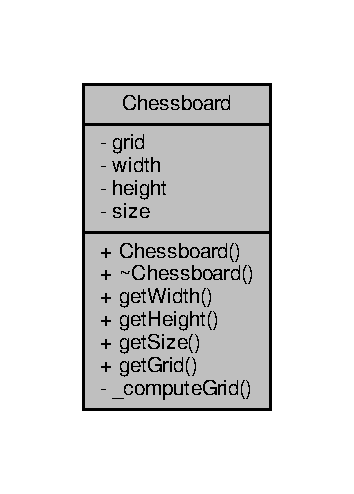
\includegraphics[width=170pt]{class_chessboard__coll__graph}
\end{center}
\end{figure}
\subsection*{Public Member Functions}
\begin{DoxyCompactItemize}
\item 
\hyperlink{class_chessboard_aa80499df26acccc4fd9d6449c1d847f0}{Chessboard} (int \hyperlink{class_chessboard_a508e83c453e3aef8af69bdb934262d83}{width}, int \hyperlink{class_chessboard_ad7baa62b4f5f47627bae49a53475a56c}{height}, float \hyperlink{class_chessboard_a898569d2e3c1e297f9915fa437c41082}{size})
\begin{DoxyCompactList}\small\item\em Constructor of \hyperlink{class_chessboard}{Chessboard} class. \end{DoxyCompactList}\item 
\hyperlink{class_chessboard_a53eac522998d8d92cca409493c773f54}{$\sim$\+Chessboard} ()
\begin{DoxyCompactList}\small\item\em Deconstructor of \hyperlink{class_chessboard}{Chessboard} class. \end{DoxyCompactList}\item 
int \hyperlink{class_chessboard_aeecfc5f0c890fec1db2a45619332459b}{get\+Width} ()
\begin{DoxyCompactList}\small\item\em Function used to obtain the width of the chessboard (number of the blocks). \end{DoxyCompactList}\item 
int \hyperlink{class_chessboard_a5cbb8122bc0f8fc08d82e0541e01f7da}{get\+Height} ()
\begin{DoxyCompactList}\small\item\em Function uesd to obtain the height of the chessboard (number of the blocks). \end{DoxyCompactList}\item 
float \hyperlink{class_chessboard_a4640a7683d77d32621fa8821f1ec3d7d}{get\+Size} ()
\begin{DoxyCompactList}\small\item\em Function used to obtain the size of the block (mm). \end{DoxyCompactList}\item 
std\+::vector$<$ cv\+::\+Point3f $>$ \hyperlink{class_chessboard_af81a2c5b8a5914ef625a7accd0f2462f}{get\+Grid} ()
\begin{DoxyCompactList}\small\item\em Function used to get the coordinates of all the corners. \end{DoxyCompactList}\end{DoxyCompactItemize}
\subsection*{Private Member Functions}
\begin{DoxyCompactItemize}
\item 
std\+::vector$<$ cv\+::\+Point3f $>$ \hyperlink{class_chessboard_a1c02a45bc0f1bf6430d648d8f63e83e4}{\+\_\+compute\+Grid} ()
\begin{DoxyCompactList}\small\item\em Function that estimates the coordinates of each corners. \end{DoxyCompactList}\end{DoxyCompactItemize}
\subsection*{Private Attributes}
\begin{DoxyCompactItemize}
\item 
std\+::vector$<$ cv\+::\+Point3f $>$ \hyperlink{class_chessboard_aa503005107b822a202c296598a81096b}{grid}
\item 
int \hyperlink{class_chessboard_a508e83c453e3aef8af69bdb934262d83}{width}
\item 
int \hyperlink{class_chessboard_ad7baa62b4f5f47627bae49a53475a56c}{height}
\item 
float \hyperlink{class_chessboard_a898569d2e3c1e297f9915fa437c41082}{size}
\end{DoxyCompactItemize}


\subsection{Detailed Description}
Creation of chessboard. 

This class wraps the creation of a chessboard. 

\subsection{Constructor \& Destructor Documentation}
\mbox{\Hypertarget{class_chessboard_aa80499df26acccc4fd9d6449c1d847f0}\label{class_chessboard_aa80499df26acccc4fd9d6449c1d847f0}} 
\index{Chessboard@{Chessboard}!Chessboard@{Chessboard}}
\index{Chessboard@{Chessboard}!Chessboard@{Chessboard}}
\subsubsection{\texorpdfstring{Chessboard()}{Chessboard()}}
{\footnotesize\ttfamily Chessboard\+::\+Chessboard (\begin{DoxyParamCaption}\item[{int}]{width,  }\item[{int}]{height,  }\item[{float}]{size }\end{DoxyParamCaption})}



Constructor of \hyperlink{class_chessboard}{Chessboard} class. 


\begin{DoxyParams}{Parameters}
{\em width} & Width of the chessboard. \\
\hline
{\em height} & Height of the chessboard. \\
\hline
{\em size} & Side length of each block. \\
\hline
\end{DoxyParams}
\mbox{\Hypertarget{class_chessboard_a53eac522998d8d92cca409493c773f54}\label{class_chessboard_a53eac522998d8d92cca409493c773f54}} 
\index{Chessboard@{Chessboard}!````~Chessboard@{$\sim$\+Chessboard}}
\index{````~Chessboard@{$\sim$\+Chessboard}!Chessboard@{Chessboard}}
\subsubsection{\texorpdfstring{$\sim$\+Chessboard()}{~Chessboard()}}
{\footnotesize\ttfamily Chessboard\+::$\sim$\+Chessboard (\begin{DoxyParamCaption}{ }\end{DoxyParamCaption})\hspace{0.3cm}{\ttfamily [inline]}}



Deconstructor of \hyperlink{class_chessboard}{Chessboard} class. 



\subsection{Member Function Documentation}
\mbox{\Hypertarget{class_chessboard_a1c02a45bc0f1bf6430d648d8f63e83e4}\label{class_chessboard_a1c02a45bc0f1bf6430d648d8f63e83e4}} 
\index{Chessboard@{Chessboard}!\+\_\+compute\+Grid@{\+\_\+compute\+Grid}}
\index{\+\_\+compute\+Grid@{\+\_\+compute\+Grid}!Chessboard@{Chessboard}}
\subsubsection{\texorpdfstring{\+\_\+compute\+Grid()}{\_computeGrid()}}
{\footnotesize\ttfamily std\+::vector$<$ cv\+::\+Point3f $>$ Chessboard\+::\+\_\+compute\+Grid (\begin{DoxyParamCaption}{ }\end{DoxyParamCaption})\hspace{0.3cm}{\ttfamily [private]}}



Function that estimates the coordinates of each corners. 

\begin{DoxyReturn}{Returns}
A vector of three-\/dimensional points. 
\end{DoxyReturn}
\mbox{\Hypertarget{class_chessboard_af81a2c5b8a5914ef625a7accd0f2462f}\label{class_chessboard_af81a2c5b8a5914ef625a7accd0f2462f}} 
\index{Chessboard@{Chessboard}!get\+Grid@{get\+Grid}}
\index{get\+Grid@{get\+Grid}!Chessboard@{Chessboard}}
\subsubsection{\texorpdfstring{get\+Grid()}{getGrid()}}
{\footnotesize\ttfamily std\+::vector$<$ cv\+::\+Point3f $>$ Chessboard\+::get\+Grid (\begin{DoxyParamCaption}{ }\end{DoxyParamCaption})}



Function used to get the coordinates of all the corners. 

\begin{DoxyReturn}{Returns}
A vector of three-\/dimensional points. 
\end{DoxyReturn}
\mbox{\Hypertarget{class_chessboard_a5cbb8122bc0f8fc08d82e0541e01f7da}\label{class_chessboard_a5cbb8122bc0f8fc08d82e0541e01f7da}} 
\index{Chessboard@{Chessboard}!get\+Height@{get\+Height}}
\index{get\+Height@{get\+Height}!Chessboard@{Chessboard}}
\subsubsection{\texorpdfstring{get\+Height()}{getHeight()}}
{\footnotesize\ttfamily int Chessboard\+::get\+Height (\begin{DoxyParamCaption}{ }\end{DoxyParamCaption})}



Function uesd to obtain the height of the chessboard (number of the blocks). 

\mbox{\Hypertarget{class_chessboard_a4640a7683d77d32621fa8821f1ec3d7d}\label{class_chessboard_a4640a7683d77d32621fa8821f1ec3d7d}} 
\index{Chessboard@{Chessboard}!get\+Size@{get\+Size}}
\index{get\+Size@{get\+Size}!Chessboard@{Chessboard}}
\subsubsection{\texorpdfstring{get\+Size()}{getSize()}}
{\footnotesize\ttfamily float Chessboard\+::get\+Size (\begin{DoxyParamCaption}{ }\end{DoxyParamCaption})}



Function used to obtain the size of the block (mm). 

\mbox{\Hypertarget{class_chessboard_aeecfc5f0c890fec1db2a45619332459b}\label{class_chessboard_aeecfc5f0c890fec1db2a45619332459b}} 
\index{Chessboard@{Chessboard}!get\+Width@{get\+Width}}
\index{get\+Width@{get\+Width}!Chessboard@{Chessboard}}
\subsubsection{\texorpdfstring{get\+Width()}{getWidth()}}
{\footnotesize\ttfamily int Chessboard\+::get\+Width (\begin{DoxyParamCaption}{ }\end{DoxyParamCaption})}



Function used to obtain the width of the chessboard (number of the blocks). 



\subsection{Member Data Documentation}
\mbox{\Hypertarget{class_chessboard_aa503005107b822a202c296598a81096b}\label{class_chessboard_aa503005107b822a202c296598a81096b}} 
\index{Chessboard@{Chessboard}!grid@{grid}}
\index{grid@{grid}!Chessboard@{Chessboard}}
\subsubsection{\texorpdfstring{grid}{grid}}
{\footnotesize\ttfamily std\+::vector$<$cv\+::\+Point3f$>$ Chessboard\+::grid\hspace{0.3cm}{\ttfamily [private]}}

The coordinates of all the corners in the chessboard. \mbox{\Hypertarget{class_chessboard_ad7baa62b4f5f47627bae49a53475a56c}\label{class_chessboard_ad7baa62b4f5f47627bae49a53475a56c}} 
\index{Chessboard@{Chessboard}!height@{height}}
\index{height@{height}!Chessboard@{Chessboard}}
\subsubsection{\texorpdfstring{height}{height}}
{\footnotesize\ttfamily int Chessboard\+::height\hspace{0.3cm}{\ttfamily [private]}}

The height of the chessboard (number of the blocks). \mbox{\Hypertarget{class_chessboard_a898569d2e3c1e297f9915fa437c41082}\label{class_chessboard_a898569d2e3c1e297f9915fa437c41082}} 
\index{Chessboard@{Chessboard}!size@{size}}
\index{size@{size}!Chessboard@{Chessboard}}
\subsubsection{\texorpdfstring{size}{size}}
{\footnotesize\ttfamily float Chessboard\+::size\hspace{0.3cm}{\ttfamily [private]}}

The size of the block. \mbox{\Hypertarget{class_chessboard_a508e83c453e3aef8af69bdb934262d83}\label{class_chessboard_a508e83c453e3aef8af69bdb934262d83}} 
\index{Chessboard@{Chessboard}!width@{width}}
\index{width@{width}!Chessboard@{Chessboard}}
\subsubsection{\texorpdfstring{width}{width}}
{\footnotesize\ttfamily int Chessboard\+::width\hspace{0.3cm}{\ttfamily [private]}}

The width of the chessboard (number of the blocks). 

The documentation for this class was generated from the following files\+:\begin{DoxyCompactItemize}
\item 
/home/bdn\+\_\+jz/bdn\+\_\+jz/camera-\/tracker-\/cpp/\+Camera\+Tracker\+Linux/include/\hyperlink{_chessboard_8h}{Chessboard.\+h}\item 
/home/bdn\+\_\+jz/bdn\+\_\+jz/camera-\/tracker-\/cpp/\+Camera\+Tracker\+Linux/src/\hyperlink{_chessboard_8cpp}{Chessboard.\+cpp}\end{DoxyCompactItemize}

\hypertarget{class_chessboard_detector}{}\section{Chessboard\+Detector Class Reference}
\label{class_chessboard_detector}\index{Chessboard\+Detector@{Chessboard\+Detector}}


Implementation of chessboard detection.  




{\ttfamily \#include $<$Chessboard\+Detector.\+h$>$}



Collaboration diagram for Chessboard\+Detector\+:\nopagebreak
\begin{figure}[H]
\begin{center}
\leavevmode
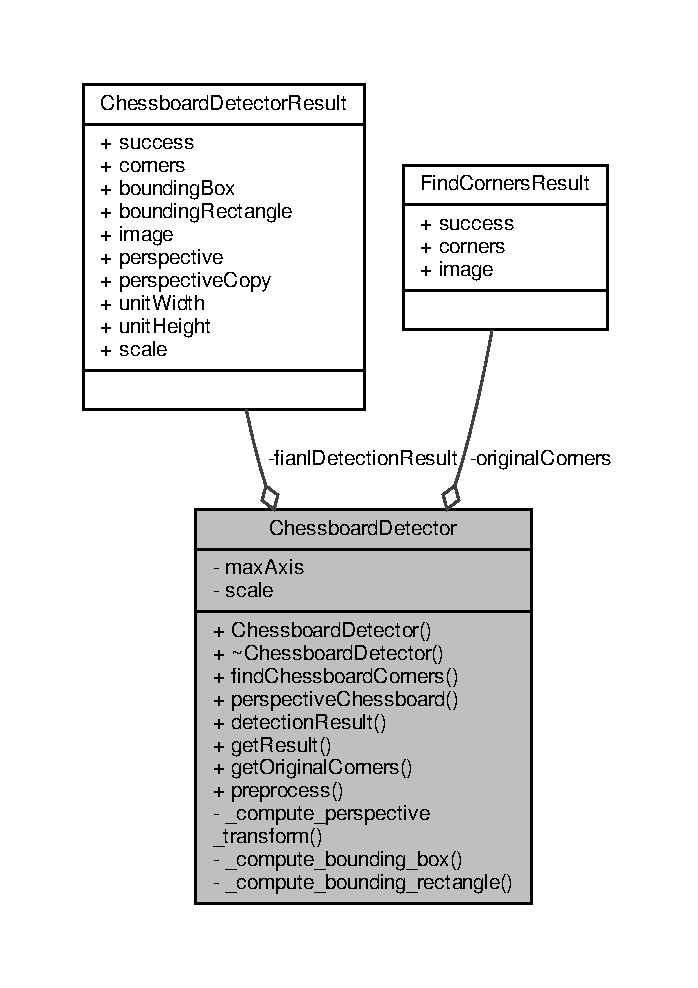
\includegraphics[width=335pt]{class_chessboard_detector__coll__graph}
\end{center}
\end{figure}
\subsection*{Public Member Functions}
\begin{DoxyCompactItemize}
\item 
\hyperlink{class_chessboard_detector_aebbd98195c5f2b06ca0f10fb65d9211e}{Chessboard\+Detector} (\hyperlink{class_chessboard}{Chessboard} chessboard, cv\+::\+Mat source\+Image)
\begin{DoxyCompactList}\small\item\em Constructor that performs the whole procedure to get the chessboard detection result. \end{DoxyCompactList}\item 
\hyperlink{class_chessboard_detector_a7db4aa40348c01899ac8be7a959d1f77}{$\sim$\+Chessboard\+Detector} ()
\begin{DoxyCompactList}\small\item\em Deconstructor of \hyperlink{class_chessboard_detector}{Chessboard\+Detector} class. \end{DoxyCompactList}\item 
\hyperlink{struct_find_corners_result}{Find\+Corners\+Result} \hyperlink{class_chessboard_detector_a4d0df2c6479f32286935577e1b0fca41}{find\+Chessboard\+Corners} (cv\+::\+Mat image, \hyperlink{class_chessboard}{Chessboard} chessboard)
\begin{DoxyCompactList}\small\item\em Function that finds the corners in the original image. \end{DoxyCompactList}\item 
\hyperlink{struct_perspective_result}{Perspective\+Result} \hyperlink{class_chessboard_detector_a591172112aeddde99db0f3dafda05b89}{perspective\+Chessboard} (\hyperlink{struct_find_corners_result}{Find\+Corners\+Result} corners)
\begin{DoxyCompactList}\small\item\em Functions that contains the whole procedure of perspective transformation. \end{DoxyCompactList}\item 
\hyperlink{struct_chessboard_detector_result}{Chessboard\+Detector\+Result} \hyperlink{class_chessboard_detector_a97550158d545864e639f0a6311f56f16}{detection\+Result} (cv\+::\+Mat original\+Image, \hyperlink{class_chessboard}{Chessboard} chessboard)
\begin{DoxyCompactList}\small\item\em Functions that returns the result of chessboard detection. \end{DoxyCompactList}\item 
\hyperlink{struct_chessboard_detector_result}{Chessboard\+Detector\+Result} \hyperlink{class_chessboard_detector_a84f8880402d0829ed6fc13ed45a141c4}{get\+Result} ()
\begin{DoxyCompactList}\small\item\em Function used to get the detection result outside the class. \end{DoxyCompactList}\item 
\hyperlink{struct_find_corners_result}{Find\+Corners\+Result} \hyperlink{class_chessboard_detector_a7f8fd52d9bb23984c0db1c4115e75043}{get\+Original\+Corners} ()
\begin{DoxyCompactList}\small\item\em Function that finds the corners in the original image. \end{DoxyCompactList}\item 
cv\+::\+Mat \hyperlink{class_chessboard_detector_a5860832e43410d526daf7415e5775aa9}{preprocess} (cv\+::\+Mat original\+Image)
\begin{DoxyCompactList}\small\item\em Function that resize the image so that the longest side has 860 pixels. \end{DoxyCompactList}\end{DoxyCompactItemize}
\subsection*{Private Member Functions}
\begin{DoxyCompactItemize}
\item 
cv\+::\+Mat \hyperlink{class_chessboard_detector_aab8f57b255da1d014e58d5e7aa984a3e}{\+\_\+compute\+\_\+perspective\+\_\+transform} (std\+::vector$<$ cv\+::\+Point2f $>$ src, std\+::vector$<$ cv\+::\+Point2f $>$ dst, cv\+::\+Mat image)
\begin{DoxyCompactList}\small\item\em Function that calculates the matrix to perfrom perspective transformation. \end{DoxyCompactList}\item 
std\+::vector$<$ cv\+::\+Point2f $>$ \hyperlink{class_chessboard_detector_af5ce25d1aa585ee9b48e705ddd9c0da1}{\+\_\+compute\+\_\+bounding\+\_\+box} (std\+::vector$<$ cv\+::\+Point2f $>$ corners)
\begin{DoxyCompactList}\small\item\em Function that estimates the coordinates of corners in the bounding box in the original image. \end{DoxyCompactList}\item 
std\+::vector$<$ cv\+::\+Point2f $>$ \hyperlink{class_chessboard_detector_a8de461985954069f87c868a930f81f2d}{\+\_\+compute\+\_\+bounding\+\_\+rectangle} (std\+::vector$<$ cv\+::\+Point2f $>$ src)
\begin{DoxyCompactList}\small\item\em Function that claculates the coordinates of corners in the assumed bounding box after perspective transformation. \end{DoxyCompactList}\end{DoxyCompactItemize}
\subsection*{Private Attributes}
\begin{DoxyCompactItemize}
\item 
\hyperlink{struct_chessboard_detector_result}{Chessboard\+Detector\+Result} \hyperlink{class_chessboard_detector_a0694ee14ff2ca2e9c0a815fd18f321cd}{fianl\+Detection\+Result}
\item 
\hyperlink{struct_find_corners_result}{Find\+Corners\+Result} \hyperlink{class_chessboard_detector_a726c92a071aa8c46d67f33c7a0760d54}{original\+Corners}
\item 
int \hyperlink{class_chessboard_detector_a5d5dc8aaf92fb5ed7e73892ad678ec96}{max\+Axis}
\item 
float \hyperlink{class_chessboard_detector_ac5594a662e5f276b5f0e5450b883efa0}{scale}
\end{DoxyCompactItemize}


\subsection{Detailed Description}
Implementation of chessboard detection. 

This class wraps the preprocessing of a image and the detection of the chessboard in the image. 

\subsection{Constructor \& Destructor Documentation}
\index{Chessboard\+Detector@{Chessboard\+Detector}!Chessboard\+Detector@{Chessboard\+Detector}}
\index{Chessboard\+Detector@{Chessboard\+Detector}!Chessboard\+Detector@{Chessboard\+Detector}}
\subsubsection[{\texorpdfstring{Chessboard\+Detector(\+Chessboard chessboard, cv\+::\+Mat source\+Image)}{ChessboardDetector(Chessboard chessboard, cv::Mat sourceImage)}}]{\setlength{\rightskip}{0pt plus 5cm}Chessboard\+Detector\+::\+Chessboard\+Detector (
\begin{DoxyParamCaption}
\item[{{\bf Chessboard}}]{chessboard, }
\item[{cv\+::\+Mat}]{source\+Image}
\end{DoxyParamCaption}
)}\hypertarget{class_chessboard_detector_aebbd98195c5f2b06ca0f10fb65d9211e}{}\label{class_chessboard_detector_aebbd98195c5f2b06ca0f10fb65d9211e}


Constructor that performs the whole procedure to get the chessboard detection result. 


\begin{DoxyParams}{Parameters}
{\em chessboard} & \hyperlink{class_chessboard}{Chessboard} to detect. \\
\hline
{\em source\+Image} & Input image. \\
\hline
\end{DoxyParams}
\index{Chessboard\+Detector@{Chessboard\+Detector}!````~Chessboard\+Detector@{$\sim$\+Chessboard\+Detector}}
\index{````~Chessboard\+Detector@{$\sim$\+Chessboard\+Detector}!Chessboard\+Detector@{Chessboard\+Detector}}
\subsubsection[{\texorpdfstring{$\sim$\+Chessboard\+Detector()}{~ChessboardDetector()}}]{\setlength{\rightskip}{0pt plus 5cm}Chessboard\+Detector\+::$\sim$\+Chessboard\+Detector (
\begin{DoxyParamCaption}
{}
\end{DoxyParamCaption}
)\hspace{0.3cm}{\ttfamily [inline]}}\hypertarget{class_chessboard_detector_a7db4aa40348c01899ac8be7a959d1f77}{}\label{class_chessboard_detector_a7db4aa40348c01899ac8be7a959d1f77}


Deconstructor of \hyperlink{class_chessboard_detector}{Chessboard\+Detector} class. 



\subsection{Member Function Documentation}
\index{Chessboard\+Detector@{Chessboard\+Detector}!\+\_\+compute\+\_\+bounding\+\_\+box@{\+\_\+compute\+\_\+bounding\+\_\+box}}
\index{\+\_\+compute\+\_\+bounding\+\_\+box@{\+\_\+compute\+\_\+bounding\+\_\+box}!Chessboard\+Detector@{Chessboard\+Detector}}
\subsubsection[{\texorpdfstring{\+\_\+compute\+\_\+bounding\+\_\+box(std\+::vector$<$ cv\+::\+Point2f $>$ corners)}{_compute_bounding_box(std::vector< cv::Point2f > corners)}}]{\setlength{\rightskip}{0pt plus 5cm}std\+::vector$<$ cv\+::\+Point2f $>$ Chessboard\+Detector\+::\+\_\+compute\+\_\+bounding\+\_\+box (
\begin{DoxyParamCaption}
\item[{std\+::vector$<$ cv\+::\+Point2f $>$}]{corners}
\end{DoxyParamCaption}
)\hspace{0.3cm}{\ttfamily [private]}}\hypertarget{class_chessboard_detector_af5ce25d1aa585ee9b48e705ddd9c0da1}{}\label{class_chessboard_detector_af5ce25d1aa585ee9b48e705ddd9c0da1}


Function that estimates the coordinates of corners in the bounding box in the original image. 


\begin{DoxyParams}{Parameters}
{\em corners} & Coordinates of the corners. \\
\hline
\end{DoxyParams}
\begin{DoxyReturn}{Returns}
a vector of two-\/dimensional points. 
\end{DoxyReturn}
\index{Chessboard\+Detector@{Chessboard\+Detector}!\+\_\+compute\+\_\+bounding\+\_\+rectangle@{\+\_\+compute\+\_\+bounding\+\_\+rectangle}}
\index{\+\_\+compute\+\_\+bounding\+\_\+rectangle@{\+\_\+compute\+\_\+bounding\+\_\+rectangle}!Chessboard\+Detector@{Chessboard\+Detector}}
\subsubsection[{\texorpdfstring{\+\_\+compute\+\_\+bounding\+\_\+rectangle(std\+::vector$<$ cv\+::\+Point2f $>$ src)}{_compute_bounding_rectangle(std::vector< cv::Point2f > src)}}]{\setlength{\rightskip}{0pt plus 5cm}std\+::vector$<$ cv\+::\+Point2f $>$ Chessboard\+Detector\+::\+\_\+compute\+\_\+bounding\+\_\+rectangle (
\begin{DoxyParamCaption}
\item[{std\+::vector$<$ cv\+::\+Point2f $>$}]{src}
\end{DoxyParamCaption}
)\hspace{0.3cm}{\ttfamily [private]}}\hypertarget{class_chessboard_detector_a8de461985954069f87c868a930f81f2d}{}\label{class_chessboard_detector_a8de461985954069f87c868a930f81f2d}


Function that claculates the coordinates of corners in the assumed bounding box after perspective transformation. 


\begin{DoxyParams}{Parameters}
{\em src} & Source points for boundding rectangle computation. \\
\hline
\end{DoxyParams}
\begin{DoxyReturn}{Returns}
a vector of two-\/dimensional points. 
\end{DoxyReturn}
\index{Chessboard\+Detector@{Chessboard\+Detector}!\+\_\+compute\+\_\+perspective\+\_\+transform@{\+\_\+compute\+\_\+perspective\+\_\+transform}}
\index{\+\_\+compute\+\_\+perspective\+\_\+transform@{\+\_\+compute\+\_\+perspective\+\_\+transform}!Chessboard\+Detector@{Chessboard\+Detector}}
\subsubsection[{\texorpdfstring{\+\_\+compute\+\_\+perspective\+\_\+transform(std\+::vector$<$ cv\+::\+Point2f $>$ src, std\+::vector$<$ cv\+::\+Point2f $>$ dst, cv\+::\+Mat image)}{_compute_perspective_transform(std::vector< cv::Point2f > src, std::vector< cv::Point2f > dst, cv::Mat image)}}]{\setlength{\rightskip}{0pt plus 5cm}cv\+::\+Mat Chessboard\+Detector\+::\+\_\+compute\+\_\+perspective\+\_\+transform (
\begin{DoxyParamCaption}
\item[{std\+::vector$<$ cv\+::\+Point2f $>$}]{src, }
\item[{std\+::vector$<$ cv\+::\+Point2f $>$}]{dst, }
\item[{cv\+::\+Mat}]{image}
\end{DoxyParamCaption}
)\hspace{0.3cm}{\ttfamily [private]}}\hypertarget{class_chessboard_detector_aab8f57b255da1d014e58d5e7aa984a3e}{}\label{class_chessboard_detector_aab8f57b255da1d014e58d5e7aa984a3e}


Function that calculates the matrix to perfrom perspective transformation. 


\begin{DoxyParams}{Parameters}
{\em src} & Source points.\+s \\
\hline
{\em dst} & Destination points. \\
\hline
{\em image} & Image before transform. \\
\hline
\end{DoxyParams}
\begin{DoxyReturn}{Returns}
an opencv matrix. 
\end{DoxyReturn}
\index{Chessboard\+Detector@{Chessboard\+Detector}!detection\+Result@{detection\+Result}}
\index{detection\+Result@{detection\+Result}!Chessboard\+Detector@{Chessboard\+Detector}}
\subsubsection[{\texorpdfstring{detection\+Result(cv\+::\+Mat original\+Image, Chessboard chessboard)}{detectionResult(cv::Mat originalImage, Chessboard chessboard)}}]{\setlength{\rightskip}{0pt plus 5cm}{\bf Chessboard\+Detector\+Result} Chessboard\+Detector\+::detection\+Result (
\begin{DoxyParamCaption}
\item[{cv\+::\+Mat}]{original\+Image, }
\item[{{\bf Chessboard}}]{chessboard}
\end{DoxyParamCaption}
)}\hypertarget{class_chessboard_detector_a97550158d545864e639f0a6311f56f16}{}\label{class_chessboard_detector_a97550158d545864e639f0a6311f56f16}


Functions that returns the result of chessboard detection. 


\begin{DoxyParams}{Parameters}
{\em original\+Image} & Input image without any preprocessing. \\
\hline
{\em chessboard} & Configuration of the chessboard. \\
\hline
\end{DoxyParams}
\begin{DoxyReturn}{Returns}
Structured data of \hyperlink{struct_chessboard_detector_result}{Chessboard\+Detector\+Result}. 
\end{DoxyReturn}
\index{Chessboard\+Detector@{Chessboard\+Detector}!find\+Chessboard\+Corners@{find\+Chessboard\+Corners}}
\index{find\+Chessboard\+Corners@{find\+Chessboard\+Corners}!Chessboard\+Detector@{Chessboard\+Detector}}
\subsubsection[{\texorpdfstring{find\+Chessboard\+Corners(cv\+::\+Mat image, Chessboard chessboard)}{findChessboardCorners(cv::Mat image, Chessboard chessboard)}}]{\setlength{\rightskip}{0pt plus 5cm}{\bf Find\+Corners\+Result} Chessboard\+Detector\+::find\+Chessboard\+Corners (
\begin{DoxyParamCaption}
\item[{cv\+::\+Mat}]{image, }
\item[{{\bf Chessboard}}]{chessboard}
\end{DoxyParamCaption}
)}\hypertarget{class_chessboard_detector_a4d0df2c6479f32286935577e1b0fca41}{}\label{class_chessboard_detector_a4d0df2c6479f32286935577e1b0fca41}


Function that finds the corners in the original image. 


\begin{DoxyParams}{Parameters}
{\em image} & Input image. \\
\hline
{\em chessboard} & Configuration of the chessboard. \\
\hline
\end{DoxyParams}
\begin{DoxyReturn}{Returns}
Structured data of \hyperlink{struct_find_corners_result}{Find\+Corners\+Result}. 
\end{DoxyReturn}
\index{Chessboard\+Detector@{Chessboard\+Detector}!get\+Original\+Corners@{get\+Original\+Corners}}
\index{get\+Original\+Corners@{get\+Original\+Corners}!Chessboard\+Detector@{Chessboard\+Detector}}
\subsubsection[{\texorpdfstring{get\+Original\+Corners()}{getOriginalCorners()}}]{\setlength{\rightskip}{0pt plus 5cm}{\bf Find\+Corners\+Result} Chessboard\+Detector\+::get\+Original\+Corners (
\begin{DoxyParamCaption}
{}
\end{DoxyParamCaption}
)}\hypertarget{class_chessboard_detector_a7f8fd52d9bb23984c0db1c4115e75043}{}\label{class_chessboard_detector_a7f8fd52d9bb23984c0db1c4115e75043}


Function that finds the corners in the original image. 

\begin{DoxyReturn}{Returns}
structure of \hyperlink{struct_find_corners_result}{Find\+Corners\+Result}. 
\end{DoxyReturn}
\index{Chessboard\+Detector@{Chessboard\+Detector}!get\+Result@{get\+Result}}
\index{get\+Result@{get\+Result}!Chessboard\+Detector@{Chessboard\+Detector}}
\subsubsection[{\texorpdfstring{get\+Result()}{getResult()}}]{\setlength{\rightskip}{0pt plus 5cm}{\bf Chessboard\+Detector\+Result} Chessboard\+Detector\+::get\+Result (
\begin{DoxyParamCaption}
{}
\end{DoxyParamCaption}
)}\hypertarget{class_chessboard_detector_a84f8880402d0829ed6fc13ed45a141c4}{}\label{class_chessboard_detector_a84f8880402d0829ed6fc13ed45a141c4}


Function used to get the detection result outside the class. 

\begin{DoxyReturn}{Returns}
structure of \hyperlink{struct_chessboard_detector_result}{Chessboard\+Detector\+Result}. 
\end{DoxyReturn}
\index{Chessboard\+Detector@{Chessboard\+Detector}!perspective\+Chessboard@{perspective\+Chessboard}}
\index{perspective\+Chessboard@{perspective\+Chessboard}!Chessboard\+Detector@{Chessboard\+Detector}}
\subsubsection[{\texorpdfstring{perspective\+Chessboard(\+Find\+Corners\+Result corners)}{perspectiveChessboard(FindCornersResult corners)}}]{\setlength{\rightskip}{0pt plus 5cm}{\bf Perspective\+Result} Chessboard\+Detector\+::perspective\+Chessboard (
\begin{DoxyParamCaption}
\item[{{\bf Find\+Corners\+Result}}]{corners}
\end{DoxyParamCaption}
)}\hypertarget{class_chessboard_detector_a591172112aeddde99db0f3dafda05b89}{}\label{class_chessboard_detector_a591172112aeddde99db0f3dafda05b89}


Functions that contains the whole procedure of perspective transformation. 


\begin{DoxyParams}{Parameters}
{\em corners} & Result of finding corners in the image. \\
\hline
\end{DoxyParams}
\begin{DoxyReturn}{Returns}
Structured data of \hyperlink{struct_perspective_result}{Perspective\+Result}. 
\end{DoxyReturn}
\index{Chessboard\+Detector@{Chessboard\+Detector}!preprocess@{preprocess}}
\index{preprocess@{preprocess}!Chessboard\+Detector@{Chessboard\+Detector}}
\subsubsection[{\texorpdfstring{preprocess(cv\+::\+Mat original\+Image)}{preprocess(cv::Mat originalImage)}}]{\setlength{\rightskip}{0pt plus 5cm}cv\+::\+Mat Chessboard\+Detector\+::preprocess (
\begin{DoxyParamCaption}
\item[{cv\+::\+Mat}]{original\+Image}
\end{DoxyParamCaption}
)}\hypertarget{class_chessboard_detector_a5860832e43410d526daf7415e5775aa9}{}\label{class_chessboard_detector_a5860832e43410d526daf7415e5775aa9}


Function that resize the image so that the longest side has 860 pixels. 


\begin{DoxyParams}{Parameters}
{\em originalimage} & Input image for preprocessing. \\
\hline
\end{DoxyParams}
\begin{DoxyReturn}{Returns}
a matrix containing all the intensity values of the pixel points. 
\end{DoxyReturn}


\subsection{Member Data Documentation}
\index{Chessboard\+Detector@{Chessboard\+Detector}!fianl\+Detection\+Result@{fianl\+Detection\+Result}}
\index{fianl\+Detection\+Result@{fianl\+Detection\+Result}!Chessboard\+Detector@{Chessboard\+Detector}}
\subsubsection[{\texorpdfstring{fianl\+Detection\+Result}{fianlDetectionResult}}]{\setlength{\rightskip}{0pt plus 5cm}{\bf Chessboard\+Detector\+Result} Chessboard\+Detector\+::fianl\+Detection\+Result\hspace{0.3cm}{\ttfamily [private]}}\hypertarget{class_chessboard_detector_a0694ee14ff2ca2e9c0a815fd18f321cd}{}\label{class_chessboard_detector_a0694ee14ff2ca2e9c0a815fd18f321cd}
Final result of chessboard detection. \index{Chessboard\+Detector@{Chessboard\+Detector}!max\+Axis@{max\+Axis}}
\index{max\+Axis@{max\+Axis}!Chessboard\+Detector@{Chessboard\+Detector}}
\subsubsection[{\texorpdfstring{max\+Axis}{maxAxis}}]{\setlength{\rightskip}{0pt plus 5cm}int Chessboard\+Detector\+::max\+Axis\hspace{0.3cm}{\ttfamily [private]}}\hypertarget{class_chessboard_detector_a5d5dc8aaf92fb5ed7e73892ad678ec96}{}\label{class_chessboard_detector_a5d5dc8aaf92fb5ed7e73892ad678ec96}
Desired maximal axis of the image after preprocessing. \index{Chessboard\+Detector@{Chessboard\+Detector}!original\+Corners@{original\+Corners}}
\index{original\+Corners@{original\+Corners}!Chessboard\+Detector@{Chessboard\+Detector}}
\subsubsection[{\texorpdfstring{original\+Corners}{originalCorners}}]{\setlength{\rightskip}{0pt plus 5cm}{\bf Find\+Corners\+Result} Chessboard\+Detector\+::original\+Corners\hspace{0.3cm}{\ttfamily [private]}}\hypertarget{class_chessboard_detector_a726c92a071aa8c46d67f33c7a0760d54}{}\label{class_chessboard_detector_a726c92a071aa8c46d67f33c7a0760d54}
Corners of the origianl image. \index{Chessboard\+Detector@{Chessboard\+Detector}!scale@{scale}}
\index{scale@{scale}!Chessboard\+Detector@{Chessboard\+Detector}}
\subsubsection[{\texorpdfstring{scale}{scale}}]{\setlength{\rightskip}{0pt plus 5cm}float Chessboard\+Detector\+::scale\hspace{0.3cm}{\ttfamily [private]}}\hypertarget{class_chessboard_detector_ac5594a662e5f276b5f0e5450b883efa0}{}\label{class_chessboard_detector_ac5594a662e5f276b5f0e5450b883efa0}
Scale used to reduce the size of the image. 

The documentation for this class was generated from the following files\+:\begin{DoxyCompactItemize}
\item 
/home/jc/\+H\+I\+W\+I/camera-\/tracker-\/cpp/\+Camera\+Tracker\+Linux/include/\hyperlink{_chessboard_detector_8h}{Chessboard\+Detector.\+h}\item 
/home/jc/\+H\+I\+W\+I/camera-\/tracker-\/cpp/\+Camera\+Tracker\+Linux/src/\hyperlink{_chessboard_detector_8cpp}{Chessboard\+Detector.\+cpp}\end{DoxyCompactItemize}

\hypertarget{struct_chessboard_detector_result}{}\section{Chessboard\+Detector\+Result Struct Reference}
\label{struct_chessboard_detector_result}\index{Chessboard\+Detector\+Result@{Chessboard\+Detector\+Result}}


Structure that contains the result of chessboard detection.  




{\ttfamily \#include $<$Chessboard\+Detector.\+h$>$}



Collaboration diagram for Chessboard\+Detector\+Result\+:\nopagebreak
\begin{figure}[H]
\begin{center}
\leavevmode
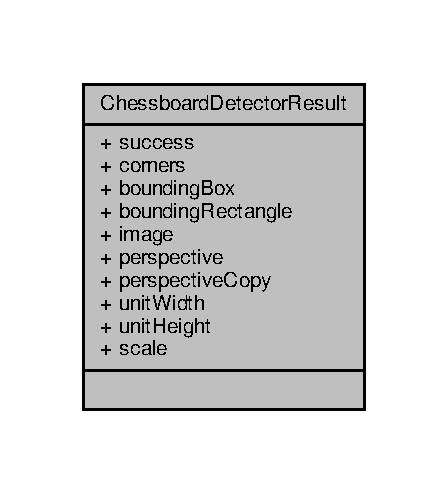
\includegraphics[width=215pt]{struct_chessboard_detector_result__coll__graph}
\end{center}
\end{figure}
\subsection*{Public Attributes}
\begin{DoxyCompactItemize}
\item 
bool \hyperlink{struct_chessboard_detector_result_a7f5e6c90f4d7b3c948d1e1ddab933df9}{success}
\item 
std\+::vector$<$ cv\+::\+Point2f $>$ \hyperlink{struct_chessboard_detector_result_a69a0fd183e694c1fb80bbad1ed2d6833}{corners}
\item 
std\+::vector$<$ cv\+::\+Point2f $>$ \hyperlink{struct_chessboard_detector_result_a6887aab98e7283ccfa4a51f8714d5260}{bounding\+Box}
\item 
std\+::vector$<$ cv\+::\+Point2f $>$ \hyperlink{struct_chessboard_detector_result_a1c1c71bb678c2eb872d9f8c4ae0a9871}{bounding\+Rectangle}
\item 
cv\+::\+Mat \hyperlink{struct_chessboard_detector_result_a9cb87f19e643fa012305b5575720332a}{image}
\item 
cv\+::\+Mat \hyperlink{struct_chessboard_detector_result_ae36efe72eb31949739d7ce8905ed2f41}{perspective}
\item 
cv\+::\+Mat \hyperlink{struct_chessboard_detector_result_a984f12b2b22c6a34a8147aa7d3d3eff0}{perspective\+Copy}
\item 
float \hyperlink{struct_chessboard_detector_result_a967889233f9ea3e34e7b215041105801}{unit\+Width}
\item 
float \hyperlink{struct_chessboard_detector_result_a95e32f26ef920afcc1e64af548120285}{unit\+Height}
\item 
float \hyperlink{struct_chessboard_detector_result_abf6c377b55ae8db5b653cb581b0baf30}{scale}
\end{DoxyCompactItemize}


\subsection{Detailed Description}
Structure that contains the result of chessboard detection. 

\subsection{Member Data Documentation}
\mbox{\Hypertarget{struct_chessboard_detector_result_a6887aab98e7283ccfa4a51f8714d5260}\label{struct_chessboard_detector_result_a6887aab98e7283ccfa4a51f8714d5260}} 
\index{Chessboard\+Detector\+Result@{Chessboard\+Detector\+Result}!bounding\+Box@{bounding\+Box}}
\index{bounding\+Box@{bounding\+Box}!Chessboard\+Detector\+Result@{Chessboard\+Detector\+Result}}
\subsubsection{\texorpdfstring{bounding\+Box}{boundingBox}}
{\footnotesize\ttfamily std\+::vector$<$cv\+::\+Point2f$>$ Chessboard\+Detector\+Result\+::bounding\+Box}

in original image. \mbox{\Hypertarget{struct_chessboard_detector_result_a1c1c71bb678c2eb872d9f8c4ae0a9871}\label{struct_chessboard_detector_result_a1c1c71bb678c2eb872d9f8c4ae0a9871}} 
\index{Chessboard\+Detector\+Result@{Chessboard\+Detector\+Result}!bounding\+Rectangle@{bounding\+Rectangle}}
\index{bounding\+Rectangle@{bounding\+Rectangle}!Chessboard\+Detector\+Result@{Chessboard\+Detector\+Result}}
\subsubsection{\texorpdfstring{bounding\+Rectangle}{boundingRectangle}}
{\footnotesize\ttfamily std\+::vector$<$cv\+::\+Point2f$>$ Chessboard\+Detector\+Result\+::bounding\+Rectangle}

after perspective transformation. \mbox{\Hypertarget{struct_chessboard_detector_result_a69a0fd183e694c1fb80bbad1ed2d6833}\label{struct_chessboard_detector_result_a69a0fd183e694c1fb80bbad1ed2d6833}} 
\index{Chessboard\+Detector\+Result@{Chessboard\+Detector\+Result}!corners@{corners}}
\index{corners@{corners}!Chessboard\+Detector\+Result@{Chessboard\+Detector\+Result}}
\subsubsection{\texorpdfstring{corners}{corners}}
{\footnotesize\ttfamily std\+::vector$<$cv\+::\+Point2f$>$ Chessboard\+Detector\+Result\+::corners}

Coordinates of the corners in the original image. \mbox{\Hypertarget{struct_chessboard_detector_result_a9cb87f19e643fa012305b5575720332a}\label{struct_chessboard_detector_result_a9cb87f19e643fa012305b5575720332a}} 
\index{Chessboard\+Detector\+Result@{Chessboard\+Detector\+Result}!image@{image}}
\index{image@{image}!Chessboard\+Detector\+Result@{Chessboard\+Detector\+Result}}
\subsubsection{\texorpdfstring{image}{image}}
{\footnotesize\ttfamily cv\+::\+Mat Chessboard\+Detector\+Result\+::image}

Original image. \mbox{\Hypertarget{struct_chessboard_detector_result_ae36efe72eb31949739d7ce8905ed2f41}\label{struct_chessboard_detector_result_ae36efe72eb31949739d7ce8905ed2f41}} 
\index{Chessboard\+Detector\+Result@{Chessboard\+Detector\+Result}!perspective@{perspective}}
\index{perspective@{perspective}!Chessboard\+Detector\+Result@{Chessboard\+Detector\+Result}}
\subsubsection{\texorpdfstring{perspective}{perspective}}
{\footnotesize\ttfamily cv\+::\+Mat Chessboard\+Detector\+Result\+::perspective}

Perspective image. \mbox{\Hypertarget{struct_chessboard_detector_result_a984f12b2b22c6a34a8147aa7d3d3eff0}\label{struct_chessboard_detector_result_a984f12b2b22c6a34a8147aa7d3d3eff0}} 
\index{Chessboard\+Detector\+Result@{Chessboard\+Detector\+Result}!perspective\+Copy@{perspective\+Copy}}
\index{perspective\+Copy@{perspective\+Copy}!Chessboard\+Detector\+Result@{Chessboard\+Detector\+Result}}
\subsubsection{\texorpdfstring{perspective\+Copy}{perspectiveCopy}}
{\footnotesize\ttfamily cv\+::\+Mat Chessboard\+Detector\+Result\+::perspective\+Copy}

Perspective image with bounding box remarked. \mbox{\Hypertarget{struct_chessboard_detector_result_abf6c377b55ae8db5b653cb581b0baf30}\label{struct_chessboard_detector_result_abf6c377b55ae8db5b653cb581b0baf30}} 
\index{Chessboard\+Detector\+Result@{Chessboard\+Detector\+Result}!scale@{scale}}
\index{scale@{scale}!Chessboard\+Detector\+Result@{Chessboard\+Detector\+Result}}
\subsubsection{\texorpdfstring{scale}{scale}}
{\footnotesize\ttfamily float Chessboard\+Detector\+Result\+::scale}

The scale used to reduce the size of the image. \mbox{\Hypertarget{struct_chessboard_detector_result_a7f5e6c90f4d7b3c948d1e1ddab933df9}\label{struct_chessboard_detector_result_a7f5e6c90f4d7b3c948d1e1ddab933df9}} 
\index{Chessboard\+Detector\+Result@{Chessboard\+Detector\+Result}!success@{success}}
\index{success@{success}!Chessboard\+Detector\+Result@{Chessboard\+Detector\+Result}}
\subsubsection{\texorpdfstring{success}{success}}
{\footnotesize\ttfamily bool Chessboard\+Detector\+Result\+::success}

Indicates whether the detection is successful \mbox{\Hypertarget{struct_chessboard_detector_result_a95e32f26ef920afcc1e64af548120285}\label{struct_chessboard_detector_result_a95e32f26ef920afcc1e64af548120285}} 
\index{Chessboard\+Detector\+Result@{Chessboard\+Detector\+Result}!unit\+Height@{unit\+Height}}
\index{unit\+Height@{unit\+Height}!Chessboard\+Detector\+Result@{Chessboard\+Detector\+Result}}
\subsubsection{\texorpdfstring{unit\+Height}{unitHeight}}
{\footnotesize\ttfamily float Chessboard\+Detector\+Result\+::unit\+Height}

The height of each block in the image. \mbox{\Hypertarget{struct_chessboard_detector_result_a967889233f9ea3e34e7b215041105801}\label{struct_chessboard_detector_result_a967889233f9ea3e34e7b215041105801}} 
\index{Chessboard\+Detector\+Result@{Chessboard\+Detector\+Result}!unit\+Width@{unit\+Width}}
\index{unit\+Width@{unit\+Width}!Chessboard\+Detector\+Result@{Chessboard\+Detector\+Result}}
\subsubsection{\texorpdfstring{unit\+Width}{unitWidth}}
{\footnotesize\ttfamily float Chessboard\+Detector\+Result\+::unit\+Width}

The width of each block in the image. 

The documentation for this struct was generated from the following file\+:\begin{DoxyCompactItemize}
\item 
/home/bdn\+\_\+jz/bdn\+\_\+jz/camera-\/tracker-\/cpp/\+Camera\+Tracker\+Linux/include/\hyperlink{_chessboard_detector_8h}{Chessboard\+Detector.\+h}\end{DoxyCompactItemize}

\hypertarget{struct_code_info}{}\section{Code\+Info Struct Reference}
\label{struct_code_info}\index{Code\+Info@{Code\+Info}}


Structure that contains the related information of the code.  




{\ttfamily \#include $<$Scanner.\+h$>$}



Collaboration diagram for Code\+Info\+:\nopagebreak
\begin{figure}[H]
\begin{center}
\leavevmode
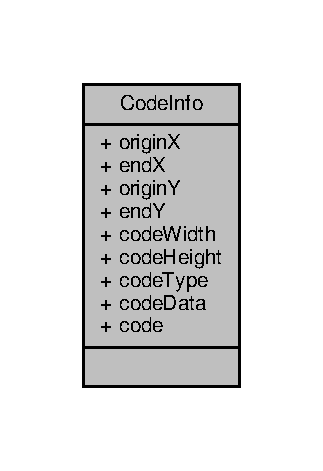
\includegraphics[width=155pt]{struct_code_info__coll__graph}
\end{center}
\end{figure}
\subsection*{Public Attributes}
\begin{DoxyCompactItemize}
\item 
float \hyperlink{struct_code_info_aaf7a04108a44c795809b1c0322f53a9b}{originX}
\item 
float \hyperlink{struct_code_info_afcbf3d398415769aba6f875c29395ec7}{endX}
\item 
float \hyperlink{struct_code_info_aa4dab88d16276786b4556f021fd192f7}{originY}
\item 
float \hyperlink{struct_code_info_a8d3d91e8e32d9294b514950029755841}{endY}
\item 
float \hyperlink{struct_code_info_ab8493ec1c1f670d1060bde6c261f9e80}{code\+Width}
\item 
float \hyperlink{struct_code_info_a8035a0d0891b25d59693e23f192e3a29}{code\+Height}
\item 
cv\+::\+String \hyperlink{struct_code_info_aa93c41fefb9505ee55963d60ec1299e7}{code\+Type}
\item 
cv\+::\+String \hyperlink{struct_code_info_a01341cc7b99f93fbdd052f6d3e5b1e20}{code\+Data}
\item 
cv\+::\+Mat \hyperlink{struct_code_info_aeaec8d442ba7cf5b8a946f3da849ebfe}{code}
\end{DoxyCompactItemize}


\subsection{Detailed Description}
Structure that contains the related information of the code. 

\subsection{Member Data Documentation}
\mbox{\Hypertarget{struct_code_info_aeaec8d442ba7cf5b8a946f3da849ebfe}\label{struct_code_info_aeaec8d442ba7cf5b8a946f3da849ebfe}} 
\index{Code\+Info@{Code\+Info}!code@{code}}
\index{code@{code}!Code\+Info@{Code\+Info}}
\subsubsection{\texorpdfstring{code}{code}}
{\footnotesize\ttfamily cv\+::\+Mat Code\+Info\+::code}

\mbox{\Hypertarget{struct_code_info_a01341cc7b99f93fbdd052f6d3e5b1e20}\label{struct_code_info_a01341cc7b99f93fbdd052f6d3e5b1e20}} 
\index{Code\+Info@{Code\+Info}!code\+Data@{code\+Data}}
\index{code\+Data@{code\+Data}!Code\+Info@{Code\+Info}}
\subsubsection{\texorpdfstring{code\+Data}{codeData}}
{\footnotesize\ttfamily cv\+::\+String Code\+Info\+::code\+Data}

\mbox{\Hypertarget{struct_code_info_a8035a0d0891b25d59693e23f192e3a29}\label{struct_code_info_a8035a0d0891b25d59693e23f192e3a29}} 
\index{Code\+Info@{Code\+Info}!code\+Height@{code\+Height}}
\index{code\+Height@{code\+Height}!Code\+Info@{Code\+Info}}
\subsubsection{\texorpdfstring{code\+Height}{codeHeight}}
{\footnotesize\ttfamily float Code\+Info\+::code\+Height}

\mbox{\Hypertarget{struct_code_info_aa93c41fefb9505ee55963d60ec1299e7}\label{struct_code_info_aa93c41fefb9505ee55963d60ec1299e7}} 
\index{Code\+Info@{Code\+Info}!code\+Type@{code\+Type}}
\index{code\+Type@{code\+Type}!Code\+Info@{Code\+Info}}
\subsubsection{\texorpdfstring{code\+Type}{codeType}}
{\footnotesize\ttfamily cv\+::\+String Code\+Info\+::code\+Type}

\mbox{\Hypertarget{struct_code_info_ab8493ec1c1f670d1060bde6c261f9e80}\label{struct_code_info_ab8493ec1c1f670d1060bde6c261f9e80}} 
\index{Code\+Info@{Code\+Info}!code\+Width@{code\+Width}}
\index{code\+Width@{code\+Width}!Code\+Info@{Code\+Info}}
\subsubsection{\texorpdfstring{code\+Width}{codeWidth}}
{\footnotesize\ttfamily float Code\+Info\+::code\+Width}

\mbox{\Hypertarget{struct_code_info_afcbf3d398415769aba6f875c29395ec7}\label{struct_code_info_afcbf3d398415769aba6f875c29395ec7}} 
\index{Code\+Info@{Code\+Info}!endX@{endX}}
\index{endX@{endX}!Code\+Info@{Code\+Info}}
\subsubsection{\texorpdfstring{endX}{endX}}
{\footnotesize\ttfamily float Code\+Info\+::endX}

\mbox{\Hypertarget{struct_code_info_a8d3d91e8e32d9294b514950029755841}\label{struct_code_info_a8d3d91e8e32d9294b514950029755841}} 
\index{Code\+Info@{Code\+Info}!endY@{endY}}
\index{endY@{endY}!Code\+Info@{Code\+Info}}
\subsubsection{\texorpdfstring{endY}{endY}}
{\footnotesize\ttfamily float Code\+Info\+::endY}

\mbox{\Hypertarget{struct_code_info_aaf7a04108a44c795809b1c0322f53a9b}\label{struct_code_info_aaf7a04108a44c795809b1c0322f53a9b}} 
\index{Code\+Info@{Code\+Info}!originX@{originX}}
\index{originX@{originX}!Code\+Info@{Code\+Info}}
\subsubsection{\texorpdfstring{originX}{originX}}
{\footnotesize\ttfamily float Code\+Info\+::originX}

\mbox{\Hypertarget{struct_code_info_aa4dab88d16276786b4556f021fd192f7}\label{struct_code_info_aa4dab88d16276786b4556f021fd192f7}} 
\index{Code\+Info@{Code\+Info}!originY@{originY}}
\index{originY@{originY}!Code\+Info@{Code\+Info}}
\subsubsection{\texorpdfstring{originY}{originY}}
{\footnotesize\ttfamily float Code\+Info\+::originY}



The documentation for this struct was generated from the following file\+:\begin{DoxyCompactItemize}
\item 
/home/bdn\+\_\+jz/bdn\+\_\+jz/\+Camera\+Tracker\+Linux/include/\hyperlink{_scanner_8h}{Scanner.\+h}\end{DoxyCompactItemize}

\hypertarget{class_code_scanner}{}\section{Code\+Scanner Class Reference}
\label{class_code_scanner}\index{Code\+Scanner@{Code\+Scanner}}


Class that contains the precedures of finding the position of code and decoding the code.  




{\ttfamily \#include $<$Scanner.\+h$>$}



Inheritance diagram for Code\+Scanner\+:\nopagebreak
\begin{figure}[H]
\begin{center}
\leavevmode
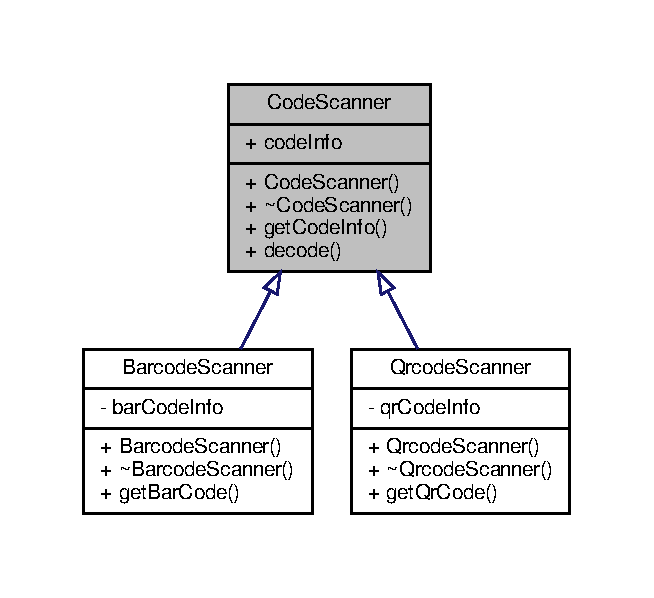
\includegraphics[width=314pt]{class_code_scanner__inherit__graph}
\end{center}
\end{figure}


Collaboration diagram for Code\+Scanner\+:\nopagebreak
\begin{figure}[H]
\begin{center}
\leavevmode
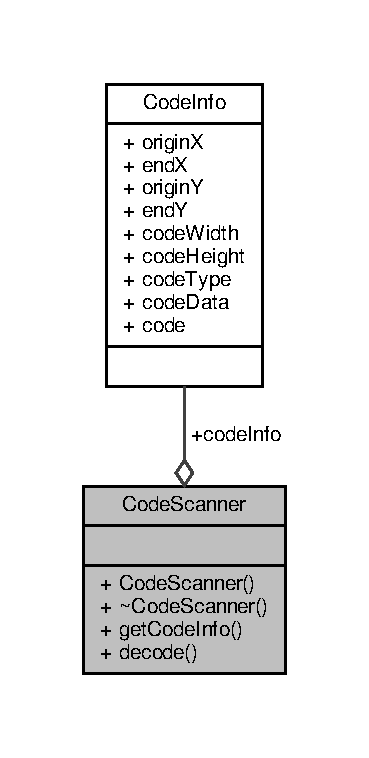
\includegraphics[width=177pt]{class_code_scanner__coll__graph}
\end{center}
\end{figure}
\subsection*{Public Member Functions}
\begin{DoxyCompactItemize}
\item 
\hyperlink{class_code_scanner_a3bcd2d58ba99d3489a82c39a7982d13b}{Code\+Scanner} ()
\begin{DoxyCompactList}\small\item\em Constructor of \hyperlink{class_code_scanner}{Code\+Scanner} class. \end{DoxyCompactList}\item 
\hyperlink{class_code_scanner_a092360e7816a81de90384495bd0f3e44}{$\sim$\+Code\+Scanner} ()
\begin{DoxyCompactList}\small\item\em Deconstructor of \hyperlink{class_code_scanner}{Code\+Scanner} class. \end{DoxyCompactList}\item 
\hyperlink{struct_code_info}{Code\+Info} \hyperlink{class_code_scanner_a8ed0db374175da430110411dac1ceba1}{get\+Code\+Info} (\hyperlink{struct_chessboard_detector_result}{Chessboard\+Detector\+Result} detection, float find\+OriginX, float find\+OriginY, float find\+EndX, float find\+EndY)
\begin{DoxyCompactList}\small\item\em Function that estimates the coordinates of code\textquotesingle{}s corners based on the upper left corner of the chessboard. \end{DoxyCompactList}\item 
\hyperlink{struct_code_info}{Code\+Info} \hyperlink{class_code_scanner_a9660d74f2750b274d92396be1cd63ab4}{decode} (\hyperlink{struct_chessboard_detector_result}{Chessboard\+Detector\+Result} detection, \hyperlink{struct_code_info}{Code\+Info} \hyperlink{class_code_scanner_a7f6371a29a0d630c9508c070f8c8966f}{code\+Info}, const std\+::string \&name)
\begin{DoxyCompactList}\small\item\em Function that decodes the code to get the type and data. \end{DoxyCompactList}\end{DoxyCompactItemize}
\subsection*{Public Attributes}
\begin{DoxyCompactItemize}
\item 
\hyperlink{struct_code_info}{Code\+Info} \hyperlink{class_code_scanner_a7f6371a29a0d630c9508c070f8c8966f}{code\+Info}
\end{DoxyCompactItemize}


\subsection{Detailed Description}
Class that contains the precedures of finding the position of code and decoding the code. 

\subsection{Constructor \& Destructor Documentation}
\mbox{\Hypertarget{class_code_scanner_a3bcd2d58ba99d3489a82c39a7982d13b}\label{class_code_scanner_a3bcd2d58ba99d3489a82c39a7982d13b}} 
\index{Code\+Scanner@{Code\+Scanner}!Code\+Scanner@{Code\+Scanner}}
\index{Code\+Scanner@{Code\+Scanner}!Code\+Scanner@{Code\+Scanner}}
\subsubsection{\texorpdfstring{Code\+Scanner()}{CodeScanner()}}
{\footnotesize\ttfamily Code\+Scanner\+::\+Code\+Scanner (\begin{DoxyParamCaption}{ }\end{DoxyParamCaption})\hspace{0.3cm}{\ttfamily [inline]}}



Constructor of \hyperlink{class_code_scanner}{Code\+Scanner} class. 

\mbox{\Hypertarget{class_code_scanner_a092360e7816a81de90384495bd0f3e44}\label{class_code_scanner_a092360e7816a81de90384495bd0f3e44}} 
\index{Code\+Scanner@{Code\+Scanner}!````~Code\+Scanner@{$\sim$\+Code\+Scanner}}
\index{````~Code\+Scanner@{$\sim$\+Code\+Scanner}!Code\+Scanner@{Code\+Scanner}}
\subsubsection{\texorpdfstring{$\sim$\+Code\+Scanner()}{~CodeScanner()}}
{\footnotesize\ttfamily Code\+Scanner\+::$\sim$\+Code\+Scanner (\begin{DoxyParamCaption}{ }\end{DoxyParamCaption})\hspace{0.3cm}{\ttfamily [inline]}}



Deconstructor of \hyperlink{class_code_scanner}{Code\+Scanner} class. 



\subsection{Member Function Documentation}
\mbox{\Hypertarget{class_code_scanner_a9660d74f2750b274d92396be1cd63ab4}\label{class_code_scanner_a9660d74f2750b274d92396be1cd63ab4}} 
\index{Code\+Scanner@{Code\+Scanner}!decode@{decode}}
\index{decode@{decode}!Code\+Scanner@{Code\+Scanner}}
\subsubsection{\texorpdfstring{decode()}{decode()}}
{\footnotesize\ttfamily \hyperlink{struct_code_info}{Code\+Info} Code\+Scanner\+::decode (\begin{DoxyParamCaption}\item[{\hyperlink{struct_chessboard_detector_result}{Chessboard\+Detector\+Result}}]{detection,  }\item[{\hyperlink{struct_code_info}{Code\+Info}}]{code\+Info,  }\item[{const std\+::string \&}]{name }\end{DoxyParamCaption})}



Function that decodes the code to get the type and data. 


\begin{DoxyParams}{Parameters}
{\em detection} & Result of chessboard detection. \\
\hline
{\em code\+Info} & Related information about the code. \\
\hline
{\em name} & Name of the code. (Only used for displaying the code) \\
\hline
\end{DoxyParams}
\begin{DoxyReturn}{Returns}
A structure of the complete information about the code 
\end{DoxyReturn}
\mbox{\Hypertarget{class_code_scanner_a8ed0db374175da430110411dac1ceba1}\label{class_code_scanner_a8ed0db374175da430110411dac1ceba1}} 
\index{Code\+Scanner@{Code\+Scanner}!get\+Code\+Info@{get\+Code\+Info}}
\index{get\+Code\+Info@{get\+Code\+Info}!Code\+Scanner@{Code\+Scanner}}
\subsubsection{\texorpdfstring{get\+Code\+Info()}{getCodeInfo()}}
{\footnotesize\ttfamily \hyperlink{struct_code_info}{Code\+Info} Code\+Scanner\+::get\+Code\+Info (\begin{DoxyParamCaption}\item[{\hyperlink{struct_chessboard_detector_result}{Chessboard\+Detector\+Result}}]{detection,  }\item[{float}]{find\+OriginX,  }\item[{float}]{find\+OriginY,  }\item[{float}]{find\+EndX,  }\item[{float}]{find\+EndY }\end{DoxyParamCaption})}



Function that estimates the coordinates of code\textquotesingle{}s corners based on the upper left corner of the chessboard. 


\begin{DoxyParams}{Parameters}
{\em detection} & Result of chessboard detection. \\
\hline
{\em find\+OriginX} & X-\/coordinate of the down left corner of the code. \\
\hline
{\em find\+OriginY} & Y-\/coordinate of the down left corner of the code. \\
\hline
{\em find\+EndX} & X-\/coordinate of the up right corner of the code. \\
\hline
{\em find\+EndY} & Y-\/coordinate of the up right corner of the code. \\
\hline
\end{DoxyParams}
\begin{DoxyReturn}{Returns}
A structure of the partial information about the code 
\end{DoxyReturn}


\subsection{Member Data Documentation}
\mbox{\Hypertarget{class_code_scanner_a7f6371a29a0d630c9508c070f8c8966f}\label{class_code_scanner_a7f6371a29a0d630c9508c070f8c8966f}} 
\index{Code\+Scanner@{Code\+Scanner}!code\+Info@{code\+Info}}
\index{code\+Info@{code\+Info}!Code\+Scanner@{Code\+Scanner}}
\subsubsection{\texorpdfstring{code\+Info}{codeInfo}}
{\footnotesize\ttfamily \hyperlink{struct_code_info}{Code\+Info} Code\+Scanner\+::code\+Info}



The documentation for this class was generated from the following files\+:\begin{DoxyCompactItemize}
\item 
/home/bdn\+\_\+jz/bdn\+\_\+jz/\+Camera\+Tracker\+Linux/include/\hyperlink{_scanner_8h}{Scanner.\+h}\item 
/home/bdn\+\_\+jz/bdn\+\_\+jz/\+Camera\+Tracker\+Linux/src/\hyperlink{_scanner_8cpp}{Scanner.\+cpp}\end{DoxyCompactItemize}

\hypertarget{class_generic_camera_1_1disconnected__exception}{}\section{Generic\+Camera\+:\+:disconnected\+\_\+exception Class Reference}
\label{class_generic_camera_1_1disconnected__exception}\index{Generic\+Camera\+::disconnected\+\_\+exception@{Generic\+Camera\+::disconnected\+\_\+exception}}


Exception if device is is disconnected Exception specificly for device disconnection, inherits from std exeception.  




{\ttfamily \#include $<$Generic\+Camera.\+h$>$}



Inheritance diagram for Generic\+Camera\+:\+:disconnected\+\_\+exception\+:\nopagebreak
\begin{figure}[H]
\begin{center}
\leavevmode
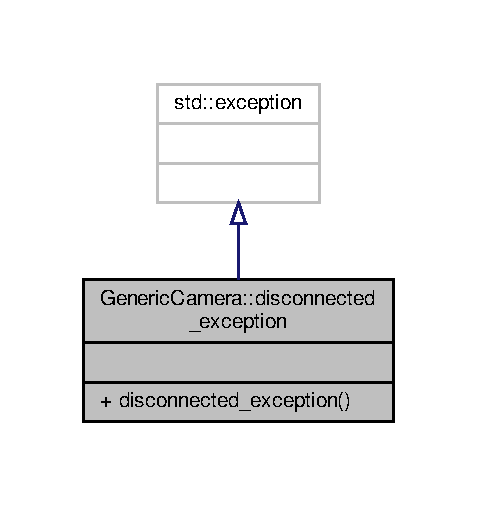
\includegraphics[width=229pt]{class_generic_camera_1_1disconnected__exception__inherit__graph}
\end{center}
\end{figure}


Collaboration diagram for Generic\+Camera\+:\+:disconnected\+\_\+exception\+:\nopagebreak
\begin{figure}[H]
\begin{center}
\leavevmode
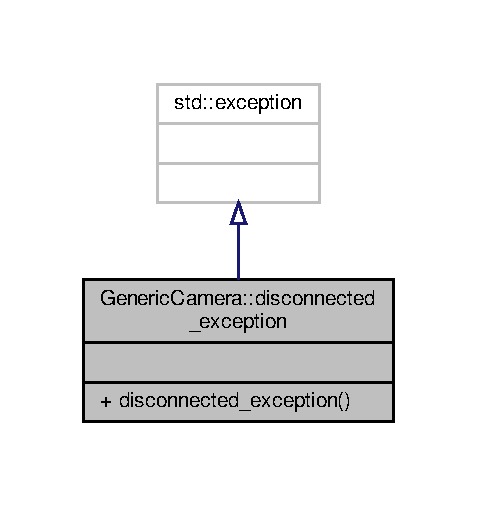
\includegraphics[width=229pt]{class_generic_camera_1_1disconnected__exception__coll__graph}
\end{center}
\end{figure}
\subsection*{Public Member Functions}
\begin{DoxyCompactItemize}
\item 
\hyperlink{class_generic_camera_1_1disconnected__exception_ac3e9d17d6848faa8bf458c19ebe21812}{disconnected\+\_\+exception} ()
\end{DoxyCompactItemize}


\subsection{Detailed Description}
Exception if device is is disconnected Exception specificly for device disconnection, inherits from std exeception. 

\subsection{Constructor \& Destructor Documentation}
\mbox{\Hypertarget{class_generic_camera_1_1disconnected__exception_ac3e9d17d6848faa8bf458c19ebe21812}\label{class_generic_camera_1_1disconnected__exception_ac3e9d17d6848faa8bf458c19ebe21812}} 
\index{Generic\+Camera\+::disconnected\+\_\+exception@{Generic\+Camera\+::disconnected\+\_\+exception}!disconnected\+\_\+exception@{disconnected\+\_\+exception}}
\index{disconnected\+\_\+exception@{disconnected\+\_\+exception}!Generic\+Camera\+::disconnected\+\_\+exception@{Generic\+Camera\+::disconnected\+\_\+exception}}
\subsubsection{\texorpdfstring{disconnected\+\_\+exception()}{disconnected\_exception()}}
{\footnotesize\ttfamily Generic\+Camera\+::disconnected\+\_\+exception\+::disconnected\+\_\+exception (\begin{DoxyParamCaption}{ }\end{DoxyParamCaption})\hspace{0.3cm}{\ttfamily [inline]}}

constructor, calling the std exception construction 
\begin{DoxyParams}[1]{Parameters}
\mbox{\tt in}  & {\em description} & descriptive error text \\
\hline
\end{DoxyParams}


The documentation for this class was generated from the following file\+:\begin{DoxyCompactItemize}
\item 
/home/bdn\+\_\+jz/bdn\+\_\+jz/camera-\/tracker-\/cpp/\+Camera\+Tracker\+Linux/include/\hyperlink{_generic_camera_8h}{Generic\+Camera.\+h}\end{DoxyCompactItemize}

\hypertarget{struct_find_corners_result}{}\section{Find\+Corners\+Result Struct Reference}
\label{struct_find_corners_result}\index{Find\+Corners\+Result@{Find\+Corners\+Result}}


Structure that contains the result of corner detection.  




{\ttfamily \#include $<$Chessboard\+Detector.\+h$>$}



Collaboration diagram for Find\+Corners\+Result\+:\nopagebreak
\begin{figure}[H]
\begin{center}
\leavevmode
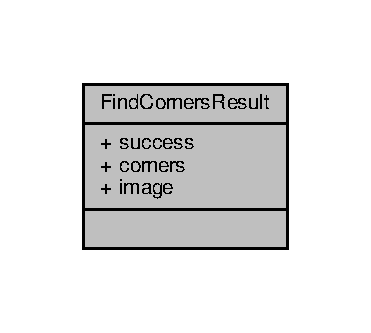
\includegraphics[width=178pt]{struct_find_corners_result__coll__graph}
\end{center}
\end{figure}
\subsection*{Public Attributes}
\begin{DoxyCompactItemize}
\item 
bool \hyperlink{struct_find_corners_result_a53a6b5d4fc0243582800d92b2bc5e706}{success}
\item 
std\+::vector$<$ cv\+::\+Point2f $>$ \hyperlink{struct_find_corners_result_a138337b67fb9eb6010ec7c9a276a009f}{corners}
\item 
cv\+::\+Mat \hyperlink{struct_find_corners_result_a8c2fd90c9f86bed108eb777fd237f113}{image}
\end{DoxyCompactItemize}


\subsection{Detailed Description}
Structure that contains the result of corner detection. 

\subsection{Member Data Documentation}
\index{Find\+Corners\+Result@{Find\+Corners\+Result}!corners@{corners}}
\index{corners@{corners}!Find\+Corners\+Result@{Find\+Corners\+Result}}
\subsubsection[{\texorpdfstring{corners}{corners}}]{\setlength{\rightskip}{0pt plus 5cm}std\+::vector$<$cv\+::\+Point2f$>$ Find\+Corners\+Result\+::corners}\hypertarget{struct_find_corners_result_a138337b67fb9eb6010ec7c9a276a009f}{}\label{struct_find_corners_result_a138337b67fb9eb6010ec7c9a276a009f}
Saves the coordinates of corners in the image coordinate system. \index{Find\+Corners\+Result@{Find\+Corners\+Result}!image@{image}}
\index{image@{image}!Find\+Corners\+Result@{Find\+Corners\+Result}}
\subsubsection[{\texorpdfstring{image}{image}}]{\setlength{\rightskip}{0pt plus 5cm}cv\+::\+Mat Find\+Corners\+Result\+::image}\hypertarget{struct_find_corners_result_a8c2fd90c9f86bed108eb777fd237f113}{}\label{struct_find_corners_result_a8c2fd90c9f86bed108eb777fd237f113}
Contains the original image taken by the camera. \index{Find\+Corners\+Result@{Find\+Corners\+Result}!success@{success}}
\index{success@{success}!Find\+Corners\+Result@{Find\+Corners\+Result}}
\subsubsection[{\texorpdfstring{success}{success}}]{\setlength{\rightskip}{0pt plus 5cm}bool Find\+Corners\+Result\+::success}\hypertarget{struct_find_corners_result_a53a6b5d4fc0243582800d92b2bc5e706}{}\label{struct_find_corners_result_a53a6b5d4fc0243582800d92b2bc5e706}
Indicates whether the searching is successful. 

The documentation for this struct was generated from the following file\+:\begin{DoxyCompactItemize}
\item 
/home/jc/\+H\+I\+W\+I/camera-\/tracker-\/cpp/\+Camera\+Tracker\+Linux/include/\hyperlink{_chessboard_detector_8h}{Chessboard\+Detector.\+h}\end{DoxyCompactItemize}

\hypertarget{class_generic_camera}{}\section{Generic\+Camera Class Reference}
\label{class_generic_camera}\index{Generic\+Camera@{Generic\+Camera}}


abstract camera base class.  




{\ttfamily \#include $<$Generic\+Camera.\+h$>$}



Inheritance diagram for Generic\+Camera\+:
\nopagebreak
\begin{figure}[H]
\begin{center}
\leavevmode
\includegraphics[height=550pt]{class_generic_camera__inherit__graph}
\end{center}
\end{figure}


Collaboration diagram for Generic\+Camera\+:
\nopagebreak
\begin{figure}[H]
\begin{center}
\leavevmode
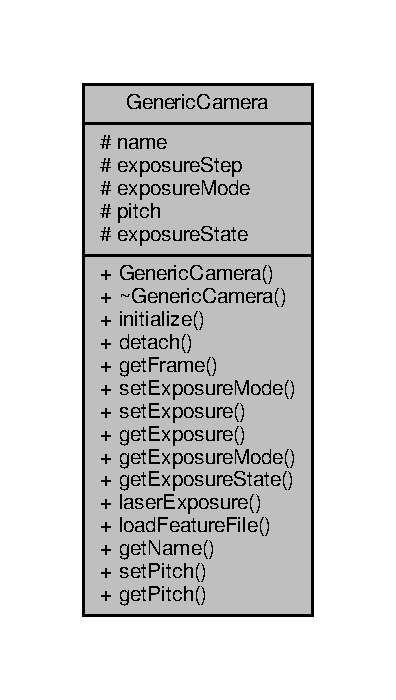
\includegraphics[width=190pt]{class_generic_camera__coll__graph}
\end{center}
\end{figure}
\subsection*{Classes}
\begin{DoxyCompactItemize}
\item 
class \hyperlink{class_generic_camera_1_1disconnected__exception}{disconnected\+\_\+exception}
\begin{DoxyCompactList}\small\item\em Exception if device is is disconnected Exception specificly for device disconnection, inherits from std exeception. \end{DoxyCompactList}\end{DoxyCompactItemize}
\subsection*{Public Member Functions}
\begin{DoxyCompactItemize}
\item 
\hyperlink{class_generic_camera_ace942cddd443bb28aeee5e49b10aa374}{Generic\+Camera} ()
\item 
virtual \hyperlink{class_generic_camera_a8a523a465c0db18b59b6113c6d308962}{$\sim$\+Generic\+Camera} ()
\item 
virtual bool \hyperlink{class_generic_camera_ad050957bbb8003fc55f4656d43347f1e}{initialize} (const std\+::string id)=0
\item 
virtual void \hyperlink{class_generic_camera_a86a91e987d6142e5417b2c07542e0aa4}{detach} (void)=0
\item 
virtual cv\+::\+Mat \hyperlink{class_generic_camera_abeaa74ba34179da70ec2c4bbb9b0d793}{get\+Frame} (void)=0
\item 
virtual bool \hyperlink{class_generic_camera_a5c3bd3ca0d691cf9026f8c91b3cf7c66}{set\+Exposure\+Mode} (\hyperlink{constants_8h_a6e920987695b1da6e2df4e41dc867e18}{Exposure\+Modes} mode)=0
\item 
virtual bool \hyperlink{class_generic_camera_a62365678e9254bde587de4a50ffb7887}{set\+Exposure} (const double time)=0
\item 
virtual double \hyperlink{class_generic_camera_ae3fe4b50577c854037b7a77dade27487}{get\+Exposure} (void) const =0
\item 
\hyperlink{constants_8h_a6e920987695b1da6e2df4e41dc867e18}{Exposure\+Modes} \hyperlink{class_generic_camera_afdd27d857471c1bca22f10520ef28a35}{get\+Exposure\+Mode} (void) const
\item 
\hyperlink{constants_8h_ae9749bac8d6973b92725af092d0a76bc}{Exposure\+States} \hyperlink{class_generic_camera_a31369d7e310827a9ac3b4366ddcbf22e}{get\+Exposure\+State} (void) const
\item 
virtual bool \hyperlink{class_generic_camera_ad20a7c33465d6791563f77a637ceed83}{laser\+Exposure} (cv\+::\+Mat \&image)
\item 
virtual void \hyperlink{class_generic_camera_a393e01ba0b1bc18ad43f00cc62ccea4e}{load\+Feature\+File} (const std\+::string filename)=0
\item 
const std\+::string \hyperlink{class_generic_camera_a7f97060cc4089fb4d8834ce8c055a561}{get\+Name} (void) const
\item 
void \hyperlink{class_generic_camera_aae87f93ed0741bbfa4881f551cd1a73c}{set\+Pitch} (double new\+Pitch)
\item 
const double \hyperlink{class_generic_camera_a429fbb0069ed11630ba5284235563f87}{get\+Pitch} (void) const
\end{DoxyCompactItemize}
\subsection*{Protected Attributes}
\begin{DoxyCompactItemize}
\item 
std\+::string \hyperlink{class_generic_camera_a12b86f8137447dd8af1864eb9bb062ee}{name}
\begin{DoxyCompactList}\small\item\em device identifier \end{DoxyCompactList}\item 
double \hyperlink{class_generic_camera_a1d0a61c9839147adaa86e9c456e3ce0c}{exposure\+Step}
\begin{DoxyCompactList}\small\item\em smallest step between two exposure times \end{DoxyCompactList}\item 
\hyperlink{constants_8h_a6e920987695b1da6e2df4e41dc867e18}{Exposure\+Modes} \hyperlink{class_generic_camera_af73c8a9c6218780d50bda3a835d16770}{exposure\+Mode}
\begin{DoxyCompactList}\small\item\em current exposure mode set \end{DoxyCompactList}\item 
double \hyperlink{class_generic_camera_a565f94ee10ad6333ca6e59a2fe8d32bb}{pitch}
\begin{DoxyCompactList}\small\item\em ratio of millimeter per pixel \end{DoxyCompactList}\item 
\hyperlink{constants_8h_ae9749bac8d6973b92725af092d0a76bc}{Exposure\+States} \hyperlink{class_generic_camera_a92600846c7691baabbc78af3b6e1cb67}{exposure\+State}
\begin{DoxyCompactList}\small\item\em current state of the exposure \end{DoxyCompactList}\end{DoxyCompactItemize}


\subsection{Detailed Description}
abstract camera base class. 

abstract camera base class where of all camera types used have to be derived, providing a unified interface 

\subsection{Constructor \& Destructor Documentation}
\mbox{\Hypertarget{class_generic_camera_ace942cddd443bb28aeee5e49b10aa374}\label{class_generic_camera_ace942cddd443bb28aeee5e49b10aa374}} 
\index{Generic\+Camera@{Generic\+Camera}!Generic\+Camera@{Generic\+Camera}}
\index{Generic\+Camera@{Generic\+Camera}!Generic\+Camera@{Generic\+Camera}}
\subsubsection{\texorpdfstring{Generic\+Camera()}{GenericCamera()}}
{\footnotesize\ttfamily Generic\+Camera\+::\+Generic\+Camera (\begin{DoxyParamCaption}{ }\end{DoxyParamCaption})}

constructor, takes no arguments \mbox{\Hypertarget{class_generic_camera_a8a523a465c0db18b59b6113c6d308962}\label{class_generic_camera_a8a523a465c0db18b59b6113c6d308962}} 
\index{Generic\+Camera@{Generic\+Camera}!````~Generic\+Camera@{$\sim$\+Generic\+Camera}}
\index{````~Generic\+Camera@{$\sim$\+Generic\+Camera}!Generic\+Camera@{Generic\+Camera}}
\subsubsection{\texorpdfstring{$\sim$\+Generic\+Camera()}{~GenericCamera()}}
{\footnotesize\ttfamily Generic\+Camera\+::$\sim$\+Generic\+Camera (\begin{DoxyParamCaption}{ }\end{DoxyParamCaption})\hspace{0.3cm}{\ttfamily [virtual]}}

virtual destructor 

\subsection{Member Function Documentation}
\mbox{\Hypertarget{class_generic_camera_a86a91e987d6142e5417b2c07542e0aa4}\label{class_generic_camera_a86a91e987d6142e5417b2c07542e0aa4}} 
\index{Generic\+Camera@{Generic\+Camera}!detach@{detach}}
\index{detach@{detach}!Generic\+Camera@{Generic\+Camera}}
\subsubsection{\texorpdfstring{detach()}{detach()}}
{\footnotesize\ttfamily virtual void Generic\+Camera\+::detach (\begin{DoxyParamCaption}\item[{void}]{ }\end{DoxyParamCaption})\hspace{0.3cm}{\ttfamily [pure virtual]}}

close the attached device, purely virtual 

Implemented in \hyperlink{class_basler_gig_e_camera_a13a51a76116cccbd537725457d83254f}{Basler\+Gig\+E\+Camera}.

\mbox{\Hypertarget{class_generic_camera_ae3fe4b50577c854037b7a77dade27487}\label{class_generic_camera_ae3fe4b50577c854037b7a77dade27487}} 
\index{Generic\+Camera@{Generic\+Camera}!get\+Exposure@{get\+Exposure}}
\index{get\+Exposure@{get\+Exposure}!Generic\+Camera@{Generic\+Camera}}
\subsubsection{\texorpdfstring{get\+Exposure()}{getExposure()}}
{\footnotesize\ttfamily virtual double Generic\+Camera\+::get\+Exposure (\begin{DoxyParamCaption}\item[{void}]{ }\end{DoxyParamCaption}) const\hspace{0.3cm}{\ttfamily [pure virtual]}}

get the current exposure time \begin{DoxyReturn}{Returns}
current exposure time in milliseconds 
\end{DoxyReturn}


Implemented in \hyperlink{class_basler_gig_e_camera_a5f7897cae5155958ecaa8b2b9196e4e6}{Basler\+Gig\+E\+Camera}.

\mbox{\Hypertarget{class_generic_camera_afdd27d857471c1bca22f10520ef28a35}\label{class_generic_camera_afdd27d857471c1bca22f10520ef28a35}} 
\index{Generic\+Camera@{Generic\+Camera}!get\+Exposure\+Mode@{get\+Exposure\+Mode}}
\index{get\+Exposure\+Mode@{get\+Exposure\+Mode}!Generic\+Camera@{Generic\+Camera}}
\subsubsection{\texorpdfstring{get\+Exposure\+Mode()}{getExposureMode()}}
{\footnotesize\ttfamily \hyperlink{constants_8h_a6e920987695b1da6e2df4e41dc867e18}{Exposure\+Modes} Generic\+Camera\+::get\+Exposure\+Mode (\begin{DoxyParamCaption}\item[{void}]{ }\end{DoxyParamCaption}) const\hspace{0.3cm}{\ttfamily [inline]}}

get the current exposure mode set \begin{DoxyReturn}{Returns}
current exposure mode 
\end{DoxyReturn}
\mbox{\Hypertarget{class_generic_camera_a31369d7e310827a9ac3b4366ddcbf22e}\label{class_generic_camera_a31369d7e310827a9ac3b4366ddcbf22e}} 
\index{Generic\+Camera@{Generic\+Camera}!get\+Exposure\+State@{get\+Exposure\+State}}
\index{get\+Exposure\+State@{get\+Exposure\+State}!Generic\+Camera@{Generic\+Camera}}
\subsubsection{\texorpdfstring{get\+Exposure\+State()}{getExposureState()}}
{\footnotesize\ttfamily \hyperlink{constants_8h_ae9749bac8d6973b92725af092d0a76bc}{Exposure\+States} Generic\+Camera\+::get\+Exposure\+State (\begin{DoxyParamCaption}\item[{void}]{ }\end{DoxyParamCaption}) const\hspace{0.3cm}{\ttfamily [inline]}}

get the current exposure state \begin{DoxyReturn}{Returns}
current exposure state 
\end{DoxyReturn}
\mbox{\Hypertarget{class_generic_camera_abeaa74ba34179da70ec2c4bbb9b0d793}\label{class_generic_camera_abeaa74ba34179da70ec2c4bbb9b0d793}} 
\index{Generic\+Camera@{Generic\+Camera}!get\+Frame@{get\+Frame}}
\index{get\+Frame@{get\+Frame}!Generic\+Camera@{Generic\+Camera}}
\subsubsection{\texorpdfstring{get\+Frame()}{getFrame()}}
{\footnotesize\ttfamily virtual cv\+::\+Mat Generic\+Camera\+::get\+Frame (\begin{DoxyParamCaption}\item[{void}]{ }\end{DoxyParamCaption})\hspace{0.3cm}{\ttfamily [pure virtual]}}

get a single frame from the camera and convert it to an open\+CV matrix, purely virtual \begin{DoxyReturn}{Returns}
acquired frame in open\+CV matrix format. 
\end{DoxyReturn}


Implemented in \hyperlink{class_basler_gig_e_camera_a8e2789aa27a9b0a8075457223afa415e}{Basler\+Gig\+E\+Camera}.

\mbox{\Hypertarget{class_generic_camera_a7f97060cc4089fb4d8834ce8c055a561}\label{class_generic_camera_a7f97060cc4089fb4d8834ce8c055a561}} 
\index{Generic\+Camera@{Generic\+Camera}!get\+Name@{get\+Name}}
\index{get\+Name@{get\+Name}!Generic\+Camera@{Generic\+Camera}}
\subsubsection{\texorpdfstring{get\+Name()}{getName()}}
{\footnotesize\ttfamily const std\+::string Generic\+Camera\+::get\+Name (\begin{DoxyParamCaption}\item[{void}]{ }\end{DoxyParamCaption}) const\hspace{0.3cm}{\ttfamily [inline]}}

get a string as a human readable identifier, i.\+e. a name \begin{DoxyReturn}{Returns}
camera name 
\end{DoxyReturn}
\mbox{\Hypertarget{class_generic_camera_a429fbb0069ed11630ba5284235563f87}\label{class_generic_camera_a429fbb0069ed11630ba5284235563f87}} 
\index{Generic\+Camera@{Generic\+Camera}!get\+Pitch@{get\+Pitch}}
\index{get\+Pitch@{get\+Pitch}!Generic\+Camera@{Generic\+Camera}}
\subsubsection{\texorpdfstring{get\+Pitch()}{getPitch()}}
{\footnotesize\ttfamily const double Generic\+Camera\+::get\+Pitch (\begin{DoxyParamCaption}\item[{void}]{ }\end{DoxyParamCaption}) const\hspace{0.3cm}{\ttfamily [inline]}}

get function for the camera pitch value \begin{DoxyReturn}{Returns}
camera pitch value 
\end{DoxyReturn}
\mbox{\Hypertarget{class_generic_camera_ad050957bbb8003fc55f4656d43347f1e}\label{class_generic_camera_ad050957bbb8003fc55f4656d43347f1e}} 
\index{Generic\+Camera@{Generic\+Camera}!initialize@{initialize}}
\index{initialize@{initialize}!Generic\+Camera@{Generic\+Camera}}
\subsubsection{\texorpdfstring{initialize()}{initialize()}}
{\footnotesize\ttfamily virtual bool Generic\+Camera\+::initialize (\begin{DoxyParamCaption}\item[{const std\+::string}]{id }\end{DoxyParamCaption})\hspace{0.3cm}{\ttfamily [pure virtual]}}

initialize the choosen device, passing the name from the list as string, purely virtual 
\begin{DoxyParams}[1]{Parameters}
\mbox{\tt in}  & {\em id} & name of the device to start \\
\hline
\end{DoxyParams}
\begin{DoxyReturn}{Returns}
success of initialization progress, i.\+e. if the camera could be activated 
\end{DoxyReturn}


Implemented in \hyperlink{class_basler_gig_e_camera_a1690e409075c423eec92a039781989df}{Basler\+Gig\+E\+Camera}.

\mbox{\Hypertarget{class_generic_camera_ad20a7c33465d6791563f77a637ceed83}\label{class_generic_camera_ad20a7c33465d6791563f77a637ceed83}} 
\index{Generic\+Camera@{Generic\+Camera}!laser\+Exposure@{laser\+Exposure}}
\index{laser\+Exposure@{laser\+Exposure}!Generic\+Camera@{Generic\+Camera}}
\subsubsection{\texorpdfstring{laser\+Exposure()}{laserExposure()}}
{\footnotesize\ttfamily bool Generic\+Camera\+::laser\+Exposure (\begin{DoxyParamCaption}\item[{cv\+::\+Mat \&}]{image }\end{DoxyParamCaption})\hspace{0.3cm}{\ttfamily [virtual]}}

set the exposure time more suited for a laser beam by checking whether any area is overexposed. the function should be called iteratively. \begin{DoxyReturn}{Returns}
true if image is properly exposed, false else 
\end{DoxyReturn}
\mbox{\Hypertarget{class_generic_camera_a393e01ba0b1bc18ad43f00cc62ccea4e}\label{class_generic_camera_a393e01ba0b1bc18ad43f00cc62ccea4e}} 
\index{Generic\+Camera@{Generic\+Camera}!load\+Feature\+File@{load\+Feature\+File}}
\index{load\+Feature\+File@{load\+Feature\+File}!Generic\+Camera@{Generic\+Camera}}
\subsubsection{\texorpdfstring{load\+Feature\+File()}{loadFeatureFile()}}
{\footnotesize\ttfamily virtual void Generic\+Camera\+::load\+Feature\+File (\begin{DoxyParamCaption}\item[{const std\+::string}]{filename }\end{DoxyParamCaption})\hspace{0.3cm}{\ttfamily [pure virtual]}}

load a file containing predefined settings, purely virtual 
\begin{DoxyParams}[1]{Parameters}
\mbox{\tt in}  & {\em filename} & name of the file \\
\hline
\end{DoxyParams}


Implemented in \hyperlink{class_basler_gig_e_camera_aa7e8cde9ecc7b2375146f41a6e35840e}{Basler\+Gig\+E\+Camera}.

\mbox{\Hypertarget{class_generic_camera_a62365678e9254bde587de4a50ffb7887}\label{class_generic_camera_a62365678e9254bde587de4a50ffb7887}} 
\index{Generic\+Camera@{Generic\+Camera}!set\+Exposure@{set\+Exposure}}
\index{set\+Exposure@{set\+Exposure}!Generic\+Camera@{Generic\+Camera}}
\subsubsection{\texorpdfstring{set\+Exposure()}{setExposure()}}
{\footnotesize\ttfamily virtual bool Generic\+Camera\+::set\+Exposure (\begin{DoxyParamCaption}\item[{const double}]{time }\end{DoxyParamCaption})\hspace{0.3cm}{\ttfamily [pure virtual]}}

manually set the exposure time of the camera, only works if the mode is not automatic, purely virtual 
\begin{DoxyParams}[1]{Parameters}
\mbox{\tt in}  & {\em time} & exposure time in milliseconds \\
\hline
\end{DoxyParams}
\begin{DoxyReturn}{Returns}
true if exposure time vcould be written to the device, false else 
\end{DoxyReturn}


Implemented in \hyperlink{class_basler_gig_e_camera_a99f9cd699aac5cb1025cb7086fbba7c0}{Basler\+Gig\+E\+Camera}.

\mbox{\Hypertarget{class_generic_camera_a5c3bd3ca0d691cf9026f8c91b3cf7c66}\label{class_generic_camera_a5c3bd3ca0d691cf9026f8c91b3cf7c66}} 
\index{Generic\+Camera@{Generic\+Camera}!set\+Exposure\+Mode@{set\+Exposure\+Mode}}
\index{set\+Exposure\+Mode@{set\+Exposure\+Mode}!Generic\+Camera@{Generic\+Camera}}
\subsubsection{\texorpdfstring{set\+Exposure\+Mode()}{setExposureMode()}}
{\footnotesize\ttfamily bool Generic\+Camera\+::set\+Exposure\+Mode (\begin{DoxyParamCaption}\item[{\hyperlink{constants_8h_a6e920987695b1da6e2df4e41dc867e18}{Exposure\+Modes}}]{mode }\end{DoxyParamCaption})\hspace{0.3cm}{\ttfamily [pure virtual]}}

set the exposure mode of the camera, choosing between automatic, manual and laser, purely virtual 
\begin{DoxyParams}[1]{Parameters}
\mbox{\tt in}  & {\em mode} & desired exposure setting \\
\hline
\end{DoxyParams}
\begin{DoxyReturn}{Returns}
true if exposure mode could be set, false else 
\end{DoxyReturn}


Implemented in \hyperlink{class_basler_gig_e_camera_a228061fb068600be59b4e83c0e8a8e50}{Basler\+Gig\+E\+Camera}.

\mbox{\Hypertarget{class_generic_camera_aae87f93ed0741bbfa4881f551cd1a73c}\label{class_generic_camera_aae87f93ed0741bbfa4881f551cd1a73c}} 
\index{Generic\+Camera@{Generic\+Camera}!set\+Pitch@{set\+Pitch}}
\index{set\+Pitch@{set\+Pitch}!Generic\+Camera@{Generic\+Camera}}
\subsubsection{\texorpdfstring{set\+Pitch()}{setPitch()}}
{\footnotesize\ttfamily void Generic\+Camera\+::set\+Pitch (\begin{DoxyParamCaption}\item[{double}]{new\+Pitch }\end{DoxyParamCaption})\hspace{0.3cm}{\ttfamily [inline]}}

lock a camera permamently to a thread 
\begin{DoxyParams}[1]{Parameters}
\mbox{\tt in}  & {\em timeout} & time in milliseconds for try\+Lock() to wait \\
\hline
\end{DoxyParams}
\begin{DoxyReturn}{Returns}
output of try\+Lock()unlocks the camera from a thread set a new camera Pitch 
\end{DoxyReturn}

\begin{DoxyParams}[1]{Parameters}
\mbox{\tt in}  & {\em new\+Pitch} & new pitch \\
\hline
\end{DoxyParams}


\subsection{Member Data Documentation}
\mbox{\Hypertarget{class_generic_camera_af73c8a9c6218780d50bda3a835d16770}\label{class_generic_camera_af73c8a9c6218780d50bda3a835d16770}} 
\index{Generic\+Camera@{Generic\+Camera}!exposure\+Mode@{exposure\+Mode}}
\index{exposure\+Mode@{exposure\+Mode}!Generic\+Camera@{Generic\+Camera}}
\subsubsection{\texorpdfstring{exposure\+Mode}{exposureMode}}
{\footnotesize\ttfamily \hyperlink{constants_8h_a6e920987695b1da6e2df4e41dc867e18}{Exposure\+Modes} Generic\+Camera\+::exposure\+Mode\hspace{0.3cm}{\ttfamily [protected]}}



current exposure mode set 

\mbox{\Hypertarget{class_generic_camera_a92600846c7691baabbc78af3b6e1cb67}\label{class_generic_camera_a92600846c7691baabbc78af3b6e1cb67}} 
\index{Generic\+Camera@{Generic\+Camera}!exposure\+State@{exposure\+State}}
\index{exposure\+State@{exposure\+State}!Generic\+Camera@{Generic\+Camera}}
\subsubsection{\texorpdfstring{exposure\+State}{exposureState}}
{\footnotesize\ttfamily \hyperlink{constants_8h_ae9749bac8d6973b92725af092d0a76bc}{Exposure\+States} Generic\+Camera\+::exposure\+State\hspace{0.3cm}{\ttfamily [protected]}}



current state of the exposure 

\mbox{\Hypertarget{class_generic_camera_a1d0a61c9839147adaa86e9c456e3ce0c}\label{class_generic_camera_a1d0a61c9839147adaa86e9c456e3ce0c}} 
\index{Generic\+Camera@{Generic\+Camera}!exposure\+Step@{exposure\+Step}}
\index{exposure\+Step@{exposure\+Step}!Generic\+Camera@{Generic\+Camera}}
\subsubsection{\texorpdfstring{exposure\+Step}{exposureStep}}
{\footnotesize\ttfamily double Generic\+Camera\+::exposure\+Step\hspace{0.3cm}{\ttfamily [protected]}}



smallest step between two exposure times 

\mbox{\Hypertarget{class_generic_camera_a12b86f8137447dd8af1864eb9bb062ee}\label{class_generic_camera_a12b86f8137447dd8af1864eb9bb062ee}} 
\index{Generic\+Camera@{Generic\+Camera}!name@{name}}
\index{name@{name}!Generic\+Camera@{Generic\+Camera}}
\subsubsection{\texorpdfstring{name}{name}}
{\footnotesize\ttfamily std\+::string Generic\+Camera\+::name\hspace{0.3cm}{\ttfamily [protected]}}



device identifier 

\mbox{\Hypertarget{class_generic_camera_a565f94ee10ad6333ca6e59a2fe8d32bb}\label{class_generic_camera_a565f94ee10ad6333ca6e59a2fe8d32bb}} 
\index{Generic\+Camera@{Generic\+Camera}!pitch@{pitch}}
\index{pitch@{pitch}!Generic\+Camera@{Generic\+Camera}}
\subsubsection{\texorpdfstring{pitch}{pitch}}
{\footnotesize\ttfamily double Generic\+Camera\+::pitch\hspace{0.3cm}{\ttfamily [protected]}}



ratio of millimeter per pixel 



The documentation for this class was generated from the following files\+:\begin{DoxyCompactItemize}
\item 
/home/bdn\+\_\+jz/bdn\+\_\+jz/camera-\/tracker-\/cpp/\+Camera\+Tracker\+Linux/include/\hyperlink{_generic_camera_8h}{Generic\+Camera.\+h}\item 
/home/bdn\+\_\+jz/bdn\+\_\+jz/camera-\/tracker-\/cpp/\+Camera\+Tracker\+Linux/src/\hyperlink{_generic_camera_8cpp}{Generic\+Camera.\+cpp}\end{DoxyCompactItemize}

\hypertarget{struct_perspective_result}{}\section{Perspective\+Result Struct Reference}
\label{struct_perspective_result}\index{Perspective\+Result@{Perspective\+Result}}


Structure that contains the result of perspective transformation.  




{\ttfamily \#include $<$Chessboard\+Detector.\+h$>$}



Collaboration diagram for Perspective\+Result\+:\nopagebreak
\begin{figure}[H]
\begin{center}
\leavevmode
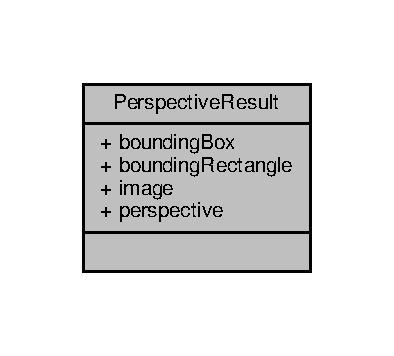
\includegraphics[width=189pt]{struct_perspective_result__coll__graph}
\end{center}
\end{figure}
\subsection*{Public Attributes}
\begin{DoxyCompactItemize}
\item 
std\+::vector$<$ cv\+::\+Point2f $>$ \hyperlink{struct_perspective_result_a2780569aa3456b68798cad4697af8647}{bounding\+Box}
\item 
std\+::vector$<$ cv\+::\+Point2f $>$ \hyperlink{struct_perspective_result_a78e1db1b132a9e364ab5f2c3b452b611}{bounding\+Rectangle}
\item 
cv\+::\+Mat \hyperlink{struct_perspective_result_a0d73af1103688870135ebb3ff7bcdbdc}{image}
\item 
cv\+::\+Mat \hyperlink{struct_perspective_result_af3e15ad54fa2f84ad2d782a2f0fd6e73}{perspective}
\end{DoxyCompactItemize}


\subsection{Detailed Description}
Structure that contains the result of perspective transformation. 

\subsection{Member Data Documentation}
\index{Perspective\+Result@{Perspective\+Result}!bounding\+Box@{bounding\+Box}}
\index{bounding\+Box@{bounding\+Box}!Perspective\+Result@{Perspective\+Result}}
\subsubsection[{\texorpdfstring{bounding\+Box}{boundingBox}}]{\setlength{\rightskip}{0pt plus 5cm}std\+::vector$<$cv\+::\+Point2f$>$ Perspective\+Result\+::bounding\+Box}\hypertarget{struct_perspective_result_a2780569aa3456b68798cad4697af8647}{}\label{struct_perspective_result_a2780569aa3456b68798cad4697af8647}
Parallelogram that surrounds all the corners. \index{Perspective\+Result@{Perspective\+Result}!bounding\+Rectangle@{bounding\+Rectangle}}
\index{bounding\+Rectangle@{bounding\+Rectangle}!Perspective\+Result@{Perspective\+Result}}
\subsubsection[{\texorpdfstring{bounding\+Rectangle}{boundingRectangle}}]{\setlength{\rightskip}{0pt plus 5cm}std\+::vector$<$cv\+::\+Point2f$>$ Perspective\+Result\+::bounding\+Rectangle}\hypertarget{struct_perspective_result_a78e1db1b132a9e364ab5f2c3b452b611}{}\label{struct_perspective_result_a78e1db1b132a9e364ab5f2c3b452b611}
Perspective tansformation of the bounding box. \index{Perspective\+Result@{Perspective\+Result}!image@{image}}
\index{image@{image}!Perspective\+Result@{Perspective\+Result}}
\subsubsection[{\texorpdfstring{image}{image}}]{\setlength{\rightskip}{0pt plus 5cm}cv\+::\+Mat Perspective\+Result\+::image}\hypertarget{struct_perspective_result_a0d73af1103688870135ebb3ff7bcdbdc}{}\label{struct_perspective_result_a0d73af1103688870135ebb3ff7bcdbdc}
Original image. \index{Perspective\+Result@{Perspective\+Result}!perspective@{perspective}}
\index{perspective@{perspective}!Perspective\+Result@{Perspective\+Result}}
\subsubsection[{\texorpdfstring{perspective}{perspective}}]{\setlength{\rightskip}{0pt plus 5cm}cv\+::\+Mat Perspective\+Result\+::perspective}\hypertarget{struct_perspective_result_af3e15ad54fa2f84ad2d782a2f0fd6e73}{}\label{struct_perspective_result_af3e15ad54fa2f84ad2d782a2f0fd6e73}
image after perspection. 

The documentation for this struct was generated from the following file\+:\begin{DoxyCompactItemize}
\item 
/home/jc/\+H\+I\+W\+I/camera-\/tracker-\/cpp/\+Camera\+Tracker\+Linux/include/\hyperlink{_chessboard_detector_8h}{Chessboard\+Detector.\+h}\end{DoxyCompactItemize}

\hypertarget{class_qrcode_scanner}{}\section{Qrcode\+Scanner Class Reference}
\label{class_qrcode_scanner}\index{Qrcode\+Scanner@{Qrcode\+Scanner}}


Class that contains the precedures of finding the position of Q\+R-\/code and decoding the Q\+R-\/code. This is a child class of \hyperlink{class_code_scanner}{Code\+Scanner}.  




{\ttfamily \#include $<$Scanner.\+h$>$}



Inheritance diagram for Qrcode\+Scanner\+:\nopagebreak
\begin{figure}[H]
\begin{center}
\leavevmode
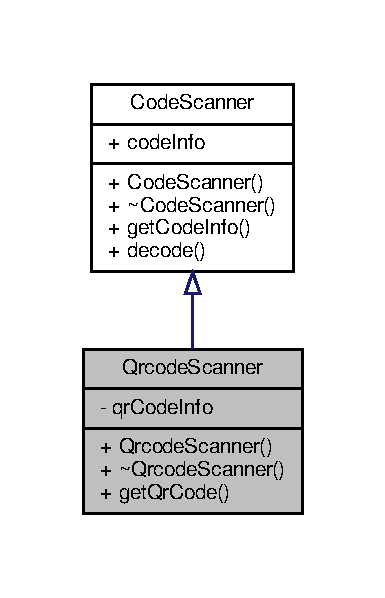
\includegraphics[width=185pt]{class_qrcode_scanner__inherit__graph}
\end{center}
\end{figure}


Collaboration diagram for Qrcode\+Scanner\+:\nopagebreak
\begin{figure}[H]
\begin{center}
\leavevmode
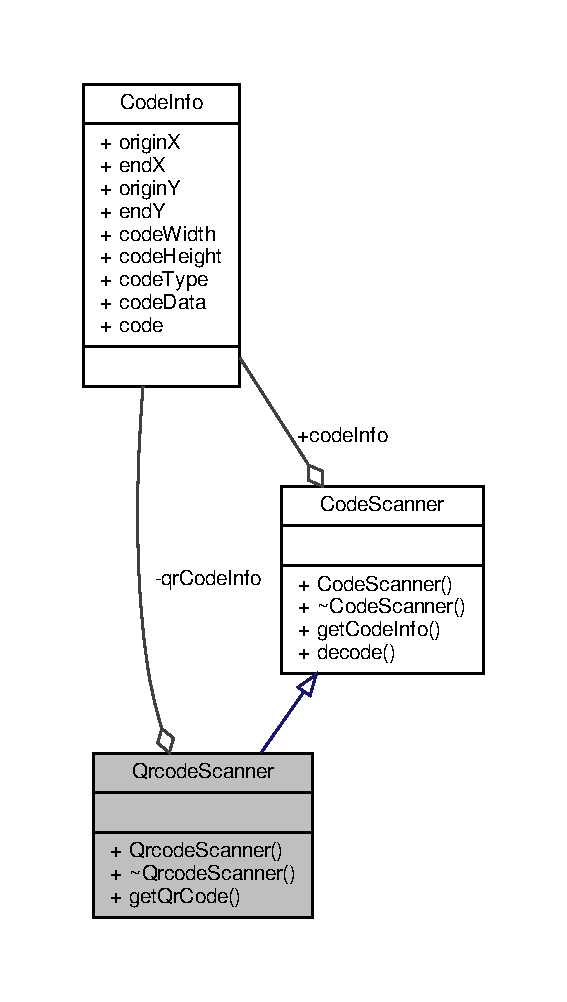
\includegraphics[width=272pt]{class_qrcode_scanner__coll__graph}
\end{center}
\end{figure}
\subsection*{Public Member Functions}
\begin{DoxyCompactItemize}
\item 
\hyperlink{class_qrcode_scanner_a92f9835aab64e4129ae9efcd72bc7518}{Qrcode\+Scanner} (\hyperlink{struct_chessboard_detector_result}{Chessboard\+Detector\+Result} detection\+Result)
\begin{DoxyCompactList}\small\item\em Constructor that performs code decoding. \end{DoxyCompactList}\item 
\hyperlink{class_qrcode_scanner_ad8670545dad4e8918b94f870f184ce80}{$\sim$\+Qrcode\+Scanner} ()
\begin{DoxyCompactList}\small\item\em Deconstructor of \hyperlink{class_qrcode_scanner}{Qrcode\+Scanner} class. \end{DoxyCompactList}\item 
\hyperlink{struct_code_info}{Code\+Info} \hyperlink{class_qrcode_scanner_ae2f75fcf7fbe48678a57c2e0eb3ca163}{get\+Qr\+Code} ()
\begin{DoxyCompactList}\small\item\em Function that is used to get code content. \end{DoxyCompactList}\end{DoxyCompactItemize}
\subsection*{Private Attributes}
\begin{DoxyCompactItemize}
\item 
\hyperlink{struct_code_info}{Code\+Info} \hyperlink{class_qrcode_scanner_af93303c867d09d136c94015610071c91}{qr\+Code\+Info}
\end{DoxyCompactItemize}
\subsection*{Additional Inherited Members}


\subsection{Detailed Description}
Class that contains the precedures of finding the position of Q\+R-\/code and decoding the Q\+R-\/code. This is a child class of \hyperlink{class_code_scanner}{Code\+Scanner}. 

\subsection{Constructor \& Destructor Documentation}
\mbox{\Hypertarget{class_qrcode_scanner_a92f9835aab64e4129ae9efcd72bc7518}\label{class_qrcode_scanner_a92f9835aab64e4129ae9efcd72bc7518}} 
\index{Qrcode\+Scanner@{Qrcode\+Scanner}!Qrcode\+Scanner@{Qrcode\+Scanner}}
\index{Qrcode\+Scanner@{Qrcode\+Scanner}!Qrcode\+Scanner@{Qrcode\+Scanner}}
\subsubsection{\texorpdfstring{Qrcode\+Scanner()}{QrcodeScanner()}}
{\footnotesize\ttfamily Qrcode\+Scanner\+::\+Qrcode\+Scanner (\begin{DoxyParamCaption}\item[{\hyperlink{struct_chessboard_detector_result}{Chessboard\+Detector\+Result}}]{detection\+Result }\end{DoxyParamCaption})}



Constructor that performs code decoding. 

\mbox{\Hypertarget{class_qrcode_scanner_ad8670545dad4e8918b94f870f184ce80}\label{class_qrcode_scanner_ad8670545dad4e8918b94f870f184ce80}} 
\index{Qrcode\+Scanner@{Qrcode\+Scanner}!````~Qrcode\+Scanner@{$\sim$\+Qrcode\+Scanner}}
\index{````~Qrcode\+Scanner@{$\sim$\+Qrcode\+Scanner}!Qrcode\+Scanner@{Qrcode\+Scanner}}
\subsubsection{\texorpdfstring{$\sim$\+Qrcode\+Scanner()}{~QrcodeScanner()}}
{\footnotesize\ttfamily Qrcode\+Scanner\+::$\sim$\+Qrcode\+Scanner (\begin{DoxyParamCaption}{ }\end{DoxyParamCaption})\hspace{0.3cm}{\ttfamily [inline]}}



Deconstructor of \hyperlink{class_qrcode_scanner}{Qrcode\+Scanner} class. 



\subsection{Member Function Documentation}
\mbox{\Hypertarget{class_qrcode_scanner_ae2f75fcf7fbe48678a57c2e0eb3ca163}\label{class_qrcode_scanner_ae2f75fcf7fbe48678a57c2e0eb3ca163}} 
\index{Qrcode\+Scanner@{Qrcode\+Scanner}!get\+Qr\+Code@{get\+Qr\+Code}}
\index{get\+Qr\+Code@{get\+Qr\+Code}!Qrcode\+Scanner@{Qrcode\+Scanner}}
\subsubsection{\texorpdfstring{get\+Qr\+Code()}{getQrCode()}}
{\footnotesize\ttfamily \hyperlink{struct_code_info}{Code\+Info} Qrcode\+Scanner\+::get\+Qr\+Code (\begin{DoxyParamCaption}{ }\end{DoxyParamCaption})}



Function that is used to get code content. 



\subsection{Member Data Documentation}
\mbox{\Hypertarget{class_qrcode_scanner_af93303c867d09d136c94015610071c91}\label{class_qrcode_scanner_af93303c867d09d136c94015610071c91}} 
\index{Qrcode\+Scanner@{Qrcode\+Scanner}!qr\+Code\+Info@{qr\+Code\+Info}}
\index{qr\+Code\+Info@{qr\+Code\+Info}!Qrcode\+Scanner@{Qrcode\+Scanner}}
\subsubsection{\texorpdfstring{qr\+Code\+Info}{qrCodeInfo}}
{\footnotesize\ttfamily \hyperlink{struct_code_info}{Code\+Info} Qrcode\+Scanner\+::qr\+Code\+Info\hspace{0.3cm}{\ttfamily [private]}}



The documentation for this class was generated from the following files\+:\begin{DoxyCompactItemize}
\item 
/home/bdn\+\_\+jz/bdn\+\_\+jz/\+Camera\+Tracker\+Linux/include/\hyperlink{_scanner_8h}{Scanner.\+h}\item 
/home/bdn\+\_\+jz/bdn\+\_\+jz/\+Camera\+Tracker\+Linux/src/\hyperlink{_scanner_8cpp}{Scanner.\+cpp}\end{DoxyCompactItemize}

\hypertarget{class_rotation_stage}{}\section{Rotation\+Stage Class Reference}
\label{class_rotation_stage}\index{Rotation\+Stage@{Rotation\+Stage}}


Control of the encoder.  




{\ttfamily \#include $<$Rotation\+Stage.\+h$>$}



Collaboration diagram for Rotation\+Stage\+:
\nopagebreak
\begin{figure}[H]
\begin{center}
\leavevmode
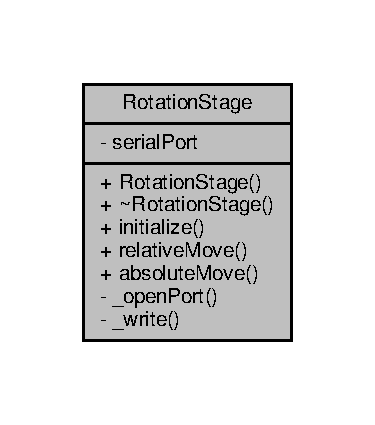
\includegraphics[width=213pt]{class_rotation_stage__coll__graph}
\end{center}
\end{figure}
\subsection*{Public Member Functions}
\begin{DoxyCompactItemize}
\item 
\hyperlink{class_rotation_stage_a14ae00fd0137138b8fa3c653498d13e9}{Rotation\+Stage} ()
\begin{DoxyCompactList}\small\item\em Construct the \hyperlink{class_rotation_stage}{Rotation\+Stage} object. \end{DoxyCompactList}\item 
\hyperlink{class_rotation_stage_a3023bae2d8de9f084036de453d8ac374}{$\sim$\+Rotation\+Stage} ()
\begin{DoxyCompactList}\small\item\em Deconstructor. \end{DoxyCompactList}\item 
void \hyperlink{class_rotation_stage_ab3e4f47bdb09f91c7c85a0fb8fc05e4b}{set\+Elevation\+Port} (std\+::string port\+Name=\char`\"{}U\+S\+B0\char`\"{})
\begin{DoxyCompactList}\small\item\em Set port for elevation. \end{DoxyCompactList}\item 
void \hyperlink{class_rotation_stage_a4fda0b9c1b8a4d6322aa48c5313a55a8}{set\+Azimuth\+Port} (std\+::string port\+Name=\char`\"{}U\+S\+B1\char`\"{})
\begin{DoxyCompactList}\small\item\em set port for azimuth \end{DoxyCompactList}\item 
void \hyperlink{class_rotation_stage_a462d2b21903430d7dfcf5fad97555195}{initialize\+Elevation} (int address=1, int home\+Search\+Type=0, float search\+Velocity=50, float search\+Time\+Out=2.\+2)
\begin{DoxyCompactList}\small\item\em Function that inializes the elevation angle. \end{DoxyCompactList}\item 
void \hyperlink{class_rotation_stage_ac1cf704b7d45ea9e1da654997d93daf7}{initialize\+Azimuth} (int address=1, int home\+Search\+Type=0, float search\+Velocity=50, float search\+Time\+Out=2.\+2)
\begin{DoxyCompactList}\small\item\em Function that inializes the azimuth angle. \end{DoxyCompactList}\item 
void \hyperlink{class_rotation_stage_aeeb1a8db6fe729db66fd7d5712dc8dee}{relative\+Move\+Elevation} (float displacement, int address=1)
\begin{DoxyCompactList}\small\item\em Function that rotates the camera tracker for a certain elevation angle. \end{DoxyCompactList}\item 
void \hyperlink{class_rotation_stage_ab1b65e7f758ef5e865098e1004002a7f}{relative\+Move\+Azimuth} (float displacement, int address=1)
\begin{DoxyCompactList}\small\item\em Function that rotates the camera tracker for a certain azimuth angle. \end{DoxyCompactList}\item 
void \hyperlink{class_rotation_stage_ad51e21e68642e5e23089f431d1242dea}{absolute\+Move\+Elevation} (float position, int address=1)
\begin{DoxyCompactList}\small\item\em Function that rotates the camera tracker to a ceratain elevation position. \end{DoxyCompactList}\item 
void \hyperlink{class_rotation_stage_a71cedba1bf3aba55bc3db7254e83b449}{absolute\+Move\+Azimuth} (float position, int address=1)
\begin{DoxyCompactList}\small\item\em Function that rotates the camera tracker to a ceratain azimuth position. \end{DoxyCompactList}\end{DoxyCompactItemize}
\subsection*{Private Member Functions}
\begin{DoxyCompactItemize}
\item 
void \hyperlink{class_rotation_stage_a8c120bd6de719b9aee263b421850bdaf}{\+\_\+open\+Port} (std\+::string U\+SB)
\begin{DoxyCompactList}\small\item\em Function used to open the corresponding port. \end{DoxyCompactList}\item 
void \hyperlink{class_rotation_stage_afb2393a3cac78176407e8e2d31a6cef4}{\+\_\+write} (std\+::string U\+SB, std\+::string code)
\begin{DoxyCompactList}\small\item\em Function used to write through a open serial port. \end{DoxyCompactList}\end{DoxyCompactItemize}
\subsection*{Private Attributes}
\begin{DoxyCompactItemize}
\item 
int \hyperlink{class_rotation_stage_a3c76fa916da6c1804f62d61e9092ec1c}{serial\+Port}
\item 
std\+::string \hyperlink{class_rotation_stage_a7e9ded06868713a22c1f630ce14c8f4e}{elevation\+Port}
\item 
std\+::string \hyperlink{class_rotation_stage_a50832a485e32836d10c4ebc2846fc93f}{azimuth\+Port}
\end{DoxyCompactItemize}


\subsection{Detailed Description}
Control of the encoder. 

This class wraps the driver controlling the encoder to rotate the camera 

\subsection{Constructor \& Destructor Documentation}
\mbox{\Hypertarget{class_rotation_stage_a14ae00fd0137138b8fa3c653498d13e9}\label{class_rotation_stage_a14ae00fd0137138b8fa3c653498d13e9}} 
\index{Rotation\+Stage@{Rotation\+Stage}!Rotation\+Stage@{Rotation\+Stage}}
\index{Rotation\+Stage@{Rotation\+Stage}!Rotation\+Stage@{Rotation\+Stage}}
\subsubsection{\texorpdfstring{Rotation\+Stage()}{RotationStage()}}
{\footnotesize\ttfamily Rotation\+Stage\+::\+Rotation\+Stage (\begin{DoxyParamCaption}{ }\end{DoxyParamCaption})\hspace{0.3cm}{\ttfamily [inline]}}



Construct the \hyperlink{class_rotation_stage}{Rotation\+Stage} object. 

\mbox{\Hypertarget{class_rotation_stage_a3023bae2d8de9f084036de453d8ac374}\label{class_rotation_stage_a3023bae2d8de9f084036de453d8ac374}} 
\index{Rotation\+Stage@{Rotation\+Stage}!````~Rotation\+Stage@{$\sim$\+Rotation\+Stage}}
\index{````~Rotation\+Stage@{$\sim$\+Rotation\+Stage}!Rotation\+Stage@{Rotation\+Stage}}
\subsubsection{\texorpdfstring{$\sim$\+Rotation\+Stage()}{~RotationStage()}}
{\footnotesize\ttfamily Rotation\+Stage\+::$\sim$\+Rotation\+Stage (\begin{DoxyParamCaption}{ }\end{DoxyParamCaption})\hspace{0.3cm}{\ttfamily [inline]}}



Deconstructor. 



\subsection{Member Function Documentation}
\mbox{\Hypertarget{class_rotation_stage_a8c120bd6de719b9aee263b421850bdaf}\label{class_rotation_stage_a8c120bd6de719b9aee263b421850bdaf}} 
\index{Rotation\+Stage@{Rotation\+Stage}!\+\_\+open\+Port@{\+\_\+open\+Port}}
\index{\+\_\+open\+Port@{\+\_\+open\+Port}!Rotation\+Stage@{Rotation\+Stage}}
\subsubsection{\texorpdfstring{\+\_\+open\+Port()}{\_openPort()}}
{\footnotesize\ttfamily void Rotation\+Stage\+::\+\_\+open\+Port (\begin{DoxyParamCaption}\item[{std\+::string}]{U\+SB }\end{DoxyParamCaption})\hspace{0.3cm}{\ttfamily [private]}}



Function used to open the corresponding port. 


\begin{DoxyParams}{Parameters}
{\em U\+SB} & File name of the corresponding serial port \\
\hline
\end{DoxyParams}
\mbox{\Hypertarget{class_rotation_stage_afb2393a3cac78176407e8e2d31a6cef4}\label{class_rotation_stage_afb2393a3cac78176407e8e2d31a6cef4}} 
\index{Rotation\+Stage@{Rotation\+Stage}!\+\_\+write@{\+\_\+write}}
\index{\+\_\+write@{\+\_\+write}!Rotation\+Stage@{Rotation\+Stage}}
\subsubsection{\texorpdfstring{\+\_\+write()}{\_write()}}
{\footnotesize\ttfamily void Rotation\+Stage\+::\+\_\+write (\begin{DoxyParamCaption}\item[{std\+::string}]{U\+SB,  }\item[{std\+::string}]{code }\end{DoxyParamCaption})\hspace{0.3cm}{\ttfamily [private]}}



Function used to write through a open serial port. 


\begin{DoxyParams}{Parameters}
{\em U\+SB} & File name of the corresponding serial port \\
\hline
{\em code} & Code to send \\
\hline
\end{DoxyParams}
\mbox{\Hypertarget{class_rotation_stage_a71cedba1bf3aba55bc3db7254e83b449}\label{class_rotation_stage_a71cedba1bf3aba55bc3db7254e83b449}} 
\index{Rotation\+Stage@{Rotation\+Stage}!absolute\+Move\+Azimuth@{absolute\+Move\+Azimuth}}
\index{absolute\+Move\+Azimuth@{absolute\+Move\+Azimuth}!Rotation\+Stage@{Rotation\+Stage}}
\subsubsection{\texorpdfstring{absolute\+Move\+Azimuth()}{absoluteMoveAzimuth()}}
{\footnotesize\ttfamily void Rotation\+Stage\+::absolute\+Move\+Azimuth (\begin{DoxyParamCaption}\item[{float}]{position,  }\item[{int}]{address = {\ttfamily 1} }\end{DoxyParamCaption})}



Function that rotates the camera tracker to a ceratain azimuth position. 


\begin{DoxyParams}{Parameters}
{\em position} & Destination of the intended rotation \\
\hline
{\em address} & Controller address \\
\hline
\end{DoxyParams}
\mbox{\Hypertarget{class_rotation_stage_ad51e21e68642e5e23089f431d1242dea}\label{class_rotation_stage_ad51e21e68642e5e23089f431d1242dea}} 
\index{Rotation\+Stage@{Rotation\+Stage}!absolute\+Move\+Elevation@{absolute\+Move\+Elevation}}
\index{absolute\+Move\+Elevation@{absolute\+Move\+Elevation}!Rotation\+Stage@{Rotation\+Stage}}
\subsubsection{\texorpdfstring{absolute\+Move\+Elevation()}{absoluteMoveElevation()}}
{\footnotesize\ttfamily void Rotation\+Stage\+::absolute\+Move\+Elevation (\begin{DoxyParamCaption}\item[{float}]{position,  }\item[{int}]{address = {\ttfamily 1} }\end{DoxyParamCaption})}



Function that rotates the camera tracker to a ceratain elevation position. 


\begin{DoxyParams}{Parameters}
{\em position} & Destination of the intended rotation \\
\hline
{\em address} & Controller address \\
\hline
\end{DoxyParams}
\mbox{\Hypertarget{class_rotation_stage_ac1cf704b7d45ea9e1da654997d93daf7}\label{class_rotation_stage_ac1cf704b7d45ea9e1da654997d93daf7}} 
\index{Rotation\+Stage@{Rotation\+Stage}!initialize\+Azimuth@{initialize\+Azimuth}}
\index{initialize\+Azimuth@{initialize\+Azimuth}!Rotation\+Stage@{Rotation\+Stage}}
\subsubsection{\texorpdfstring{initialize\+Azimuth()}{initializeAzimuth()}}
{\footnotesize\ttfamily void Rotation\+Stage\+::initialize\+Azimuth (\begin{DoxyParamCaption}\item[{int}]{address = {\ttfamily 1},  }\item[{int}]{home\+Search\+Type = {\ttfamily 0},  }\item[{float}]{search\+Velocity = {\ttfamily 50},  }\item[{float}]{search\+Time\+Out = {\ttfamily 2.2} }\end{DoxyParamCaption})}



Function that inializes the azimuth angle. 


\begin{DoxyParams}{Parameters}
{\em address} & Controller address \\
\hline
{\em home\+Search\+Type} & Type of home search, search velocity \\
\hline
{\em search\+Velocity} & Velocity of home search \\
\hline
{\em search\+Time\+Out} & Home search time-\/out \\
\hline
\end{DoxyParams}
\mbox{\Hypertarget{class_rotation_stage_a462d2b21903430d7dfcf5fad97555195}\label{class_rotation_stage_a462d2b21903430d7dfcf5fad97555195}} 
\index{Rotation\+Stage@{Rotation\+Stage}!initialize\+Elevation@{initialize\+Elevation}}
\index{initialize\+Elevation@{initialize\+Elevation}!Rotation\+Stage@{Rotation\+Stage}}
\subsubsection{\texorpdfstring{initialize\+Elevation()}{initializeElevation()}}
{\footnotesize\ttfamily void Rotation\+Stage\+::initialize\+Elevation (\begin{DoxyParamCaption}\item[{int}]{address = {\ttfamily 1},  }\item[{int}]{home\+Search\+Type = {\ttfamily 0},  }\item[{float}]{search\+Velocity = {\ttfamily 50},  }\item[{float}]{search\+Time\+Out = {\ttfamily 2.2} }\end{DoxyParamCaption})}



Function that inializes the elevation angle. 


\begin{DoxyParams}{Parameters}
{\em address} & Controller address \\
\hline
{\em home\+Search\+Type} & Type of home search, search velocity \\
\hline
{\em search\+Velocity} & Velocity of home search \\
\hline
{\em search\+Time\+Out} & Home search time-\/out \\
\hline
\end{DoxyParams}
\mbox{\Hypertarget{class_rotation_stage_ab1b65e7f758ef5e865098e1004002a7f}\label{class_rotation_stage_ab1b65e7f758ef5e865098e1004002a7f}} 
\index{Rotation\+Stage@{Rotation\+Stage}!relative\+Move\+Azimuth@{relative\+Move\+Azimuth}}
\index{relative\+Move\+Azimuth@{relative\+Move\+Azimuth}!Rotation\+Stage@{Rotation\+Stage}}
\subsubsection{\texorpdfstring{relative\+Move\+Azimuth()}{relativeMoveAzimuth()}}
{\footnotesize\ttfamily void Rotation\+Stage\+::relative\+Move\+Azimuth (\begin{DoxyParamCaption}\item[{float}]{displacement,  }\item[{int}]{address = {\ttfamily 1} }\end{DoxyParamCaption})}



Function that rotates the camera tracker for a certain azimuth angle. 


\begin{DoxyParams}{Parameters}
{\em displacement} & Displacement of the intended rotation \\
\hline
{\em address} & Controller address \\
\hline
\end{DoxyParams}
\mbox{\Hypertarget{class_rotation_stage_aeeb1a8db6fe729db66fd7d5712dc8dee}\label{class_rotation_stage_aeeb1a8db6fe729db66fd7d5712dc8dee}} 
\index{Rotation\+Stage@{Rotation\+Stage}!relative\+Move\+Elevation@{relative\+Move\+Elevation}}
\index{relative\+Move\+Elevation@{relative\+Move\+Elevation}!Rotation\+Stage@{Rotation\+Stage}}
\subsubsection{\texorpdfstring{relative\+Move\+Elevation()}{relativeMoveElevation()}}
{\footnotesize\ttfamily void Rotation\+Stage\+::relative\+Move\+Elevation (\begin{DoxyParamCaption}\item[{float}]{displacement,  }\item[{int}]{address = {\ttfamily 1} }\end{DoxyParamCaption})}



Function that rotates the camera tracker for a certain elevation angle. 


\begin{DoxyParams}{Parameters}
{\em displacement} & Displacement of the intended rotation \\
\hline
{\em address} & Controller address \\
\hline
\end{DoxyParams}
\mbox{\Hypertarget{class_rotation_stage_a4fda0b9c1b8a4d6322aa48c5313a55a8}\label{class_rotation_stage_a4fda0b9c1b8a4d6322aa48c5313a55a8}} 
\index{Rotation\+Stage@{Rotation\+Stage}!set\+Azimuth\+Port@{set\+Azimuth\+Port}}
\index{set\+Azimuth\+Port@{set\+Azimuth\+Port}!Rotation\+Stage@{Rotation\+Stage}}
\subsubsection{\texorpdfstring{set\+Azimuth\+Port()}{setAzimuthPort()}}
{\footnotesize\ttfamily void Rotation\+Stage\+::set\+Azimuth\+Port (\begin{DoxyParamCaption}\item[{std\+::string}]{port\+Name = {\ttfamily \char`\"{}USB1\char`\"{}} }\end{DoxyParamCaption})}



set port for azimuth 


\begin{DoxyParams}{Parameters}
{\em port\+Name} & Name of the port for azimuth \\
\hline
\end{DoxyParams}
\mbox{\Hypertarget{class_rotation_stage_ab3e4f47bdb09f91c7c85a0fb8fc05e4b}\label{class_rotation_stage_ab3e4f47bdb09f91c7c85a0fb8fc05e4b}} 
\index{Rotation\+Stage@{Rotation\+Stage}!set\+Elevation\+Port@{set\+Elevation\+Port}}
\index{set\+Elevation\+Port@{set\+Elevation\+Port}!Rotation\+Stage@{Rotation\+Stage}}
\subsubsection{\texorpdfstring{set\+Elevation\+Port()}{setElevationPort()}}
{\footnotesize\ttfamily void Rotation\+Stage\+::set\+Elevation\+Port (\begin{DoxyParamCaption}\item[{std\+::string}]{port\+Name = {\ttfamily \char`\"{}USB0\char`\"{}} }\end{DoxyParamCaption})}



Set port for elevation. 


\begin{DoxyParams}{Parameters}
{\em port\+Name} & Name of the port for elevation \\
\hline
\end{DoxyParams}


\subsection{Member Data Documentation}
\mbox{\Hypertarget{class_rotation_stage_a50832a485e32836d10c4ebc2846fc93f}\label{class_rotation_stage_a50832a485e32836d10c4ebc2846fc93f}} 
\index{Rotation\+Stage@{Rotation\+Stage}!azimuth\+Port@{azimuth\+Port}}
\index{azimuth\+Port@{azimuth\+Port}!Rotation\+Stage@{Rotation\+Stage}}
\subsubsection{\texorpdfstring{azimuth\+Port}{azimuthPort}}
{\footnotesize\ttfamily std\+::string Rotation\+Stage\+::azimuth\+Port\hspace{0.3cm}{\ttfamily [private]}}

\mbox{\Hypertarget{class_rotation_stage_a7e9ded06868713a22c1f630ce14c8f4e}\label{class_rotation_stage_a7e9ded06868713a22c1f630ce14c8f4e}} 
\index{Rotation\+Stage@{Rotation\+Stage}!elevation\+Port@{elevation\+Port}}
\index{elevation\+Port@{elevation\+Port}!Rotation\+Stage@{Rotation\+Stage}}
\subsubsection{\texorpdfstring{elevation\+Port}{elevationPort}}
{\footnotesize\ttfamily std\+::string Rotation\+Stage\+::elevation\+Port\hspace{0.3cm}{\ttfamily [private]}}

\mbox{\Hypertarget{class_rotation_stage_a3c76fa916da6c1804f62d61e9092ec1c}\label{class_rotation_stage_a3c76fa916da6c1804f62d61e9092ec1c}} 
\index{Rotation\+Stage@{Rotation\+Stage}!serial\+Port@{serial\+Port}}
\index{serial\+Port@{serial\+Port}!Rotation\+Stage@{Rotation\+Stage}}
\subsubsection{\texorpdfstring{serial\+Port}{serialPort}}
{\footnotesize\ttfamily int Rotation\+Stage\+::serial\+Port\hspace{0.3cm}{\ttfamily [private]}}



The documentation for this class was generated from the following files\+:\begin{DoxyCompactItemize}
\item 
/home/bdn\+\_\+jz/bdn\+\_\+jz/camera-\/tracker-\/cpp/\+Camera\+Tracker\+Linux/include/\hyperlink{_rotation_stage_8h}{Rotation\+Stage.\+h}\item 
/home/bdn\+\_\+jz/bdn\+\_\+jz/camera-\/tracker-\/cpp/\+Camera\+Tracker\+Linux/src/\hyperlink{_rotation_stage_8cpp}{Rotation\+Stage.\+cpp}\end{DoxyCompactItemize}

\hypertarget{class_timed_frame}{}\section{Timed\+Frame Class Reference}
\label{class_timed_frame}\index{Timed\+Frame@{Timed\+Frame}}


{\ttfamily \#include $<$Timed\+Frame.\+h$>$}



Collaboration diagram for Timed\+Frame\+:\nopagebreak
\begin{figure}[H]
\begin{center}
\leavevmode
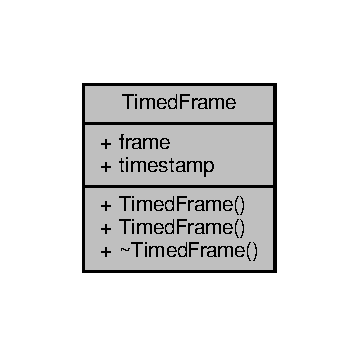
\includegraphics[width=172pt]{class_timed_frame__coll__graph}
\end{center}
\end{figure}
\subsection*{Public Member Functions}
\begin{DoxyCompactItemize}
\item 
\hyperlink{class_timed_frame_ab490571187c0ff75b843cc40245990d6}{Timed\+Frame} ()
\item 
\hyperlink{class_timed_frame_aeb70857af8b4f157785c6e0d3fcc8d53}{Timed\+Frame} (cv\+::\+Mat \hyperlink{class_timed_frame_a4c73ac094ec94f9be6558208b4916a36}{frame}, double \hyperlink{class_timed_frame_a126b8150949e1bd734778de55496b90c}{timestamp})
\item 
\hyperlink{class_timed_frame_a4be9ac0c21706f905a503fa035fd2e68}{$\sim$\+Timed\+Frame} ()
\end{DoxyCompactItemize}
\subsection*{Public Attributes}
\begin{DoxyCompactItemize}
\item 
cv\+::\+Mat \hyperlink{class_timed_frame_a4c73ac094ec94f9be6558208b4916a36}{frame}
\item 
double \hyperlink{class_timed_frame_a126b8150949e1bd734778de55496b90c}{timestamp}
\end{DoxyCompactItemize}


\subsection{Constructor \& Destructor Documentation}
\mbox{\Hypertarget{class_timed_frame_ab490571187c0ff75b843cc40245990d6}\label{class_timed_frame_ab490571187c0ff75b843cc40245990d6}} 
\index{Timed\+Frame@{Timed\+Frame}!Timed\+Frame@{Timed\+Frame}}
\index{Timed\+Frame@{Timed\+Frame}!Timed\+Frame@{Timed\+Frame}}
\subsubsection{\texorpdfstring{Timed\+Frame()}{TimedFrame()}\hspace{0.1cm}{\footnotesize\ttfamily [1/2]}}
{\footnotesize\ttfamily Timed\+Frame\+::\+Timed\+Frame (\begin{DoxyParamCaption}{ }\end{DoxyParamCaption})}

\mbox{\Hypertarget{class_timed_frame_aeb70857af8b4f157785c6e0d3fcc8d53}\label{class_timed_frame_aeb70857af8b4f157785c6e0d3fcc8d53}} 
\index{Timed\+Frame@{Timed\+Frame}!Timed\+Frame@{Timed\+Frame}}
\index{Timed\+Frame@{Timed\+Frame}!Timed\+Frame@{Timed\+Frame}}
\subsubsection{\texorpdfstring{Timed\+Frame()}{TimedFrame()}\hspace{0.1cm}{\footnotesize\ttfamily [2/2]}}
{\footnotesize\ttfamily Timed\+Frame\+::\+Timed\+Frame (\begin{DoxyParamCaption}\item[{cv\+::\+Mat}]{frame,  }\item[{double}]{timestamp }\end{DoxyParamCaption})}

\mbox{\Hypertarget{class_timed_frame_a4be9ac0c21706f905a503fa035fd2e68}\label{class_timed_frame_a4be9ac0c21706f905a503fa035fd2e68}} 
\index{Timed\+Frame@{Timed\+Frame}!````~Timed\+Frame@{$\sim$\+Timed\+Frame}}
\index{````~Timed\+Frame@{$\sim$\+Timed\+Frame}!Timed\+Frame@{Timed\+Frame}}
\subsubsection{\texorpdfstring{$\sim$\+Timed\+Frame()}{~TimedFrame()}}
{\footnotesize\ttfamily Timed\+Frame\+::$\sim$\+Timed\+Frame (\begin{DoxyParamCaption}{ }\end{DoxyParamCaption})\hspace{0.3cm}{\ttfamily [inline]}}



\subsection{Member Data Documentation}
\mbox{\Hypertarget{class_timed_frame_a4c73ac094ec94f9be6558208b4916a36}\label{class_timed_frame_a4c73ac094ec94f9be6558208b4916a36}} 
\index{Timed\+Frame@{Timed\+Frame}!frame@{frame}}
\index{frame@{frame}!Timed\+Frame@{Timed\+Frame}}
\subsubsection{\texorpdfstring{frame}{frame}}
{\footnotesize\ttfamily cv\+::\+Mat Timed\+Frame\+::frame}

\mbox{\Hypertarget{class_timed_frame_a126b8150949e1bd734778de55496b90c}\label{class_timed_frame_a126b8150949e1bd734778de55496b90c}} 
\index{Timed\+Frame@{Timed\+Frame}!timestamp@{timestamp}}
\index{timestamp@{timestamp}!Timed\+Frame@{Timed\+Frame}}
\subsubsection{\texorpdfstring{timestamp}{timestamp}}
{\footnotesize\ttfamily double Timed\+Frame\+::timestamp}



The documentation for this class was generated from the following files\+:\begin{DoxyCompactItemize}
\item 
/home/bdn\+\_\+jz/bdn\+\_\+jz/\+Camera\+Tracker\+Linux/include/\hyperlink{_timed_frame_8h}{Timed\+Frame.\+h}\item 
/home/bdn\+\_\+jz/bdn\+\_\+jz/\+Camera\+Tracker\+Linux/src/\hyperlink{_timed_frame_8cpp}{Timed\+Frame.\+cpp}\end{DoxyCompactItemize}

\chapter{File Documentation}
\hypertarget{_c_make_c_compiler_id_8c}{}\section{/home/bdn\+\_\+jz/bdn\+\_\+jz/\+Camera\+Tracker\+Linux/build/\+C\+Make\+Files/3.10.2/\+Compiler\+Id\+C/\+C\+Make\+C\+Compiler\+Id.c File Reference}
\label{_c_make_c_compiler_id_8c}\index{/home/bdn\+\_\+jz/bdn\+\_\+jz/\+Camera\+Tracker\+Linux/build/\+C\+Make\+Files/3.\+10.\+2/\+Compiler\+Id\+C/\+C\+Make\+C\+Compiler\+Id.\+c@{/home/bdn\+\_\+jz/bdn\+\_\+jz/\+Camera\+Tracker\+Linux/build/\+C\+Make\+Files/3.\+10.\+2/\+Compiler\+Id\+C/\+C\+Make\+C\+Compiler\+Id.\+c}}
\subsection*{Macros}
\begin{DoxyCompactItemize}
\item 
\#define \hyperlink{_c_make_c_compiler_id_8c_a81dee0709ded976b2e0319239f72d174}{C\+O\+M\+P\+I\+L\+E\+R\+\_\+\+ID}~\char`\"{}\char`\"{}
\item 
\#define \hyperlink{_c_make_c_compiler_id_8c_a2ae9b72bb13abaabfcf2ee0ba7d3fa1d}{S\+T\+R\+I\+N\+G\+I\+F\+Y\+\_\+\+H\+E\+L\+P\+ER}(X)~\#X
\item 
\#define \hyperlink{_c_make_c_compiler_id_8c_a43e1cad902b6477bec893cb6430bd6c8}{S\+T\+R\+I\+N\+G\+I\+FY}(X)~\hyperlink{_c_make_c_x_x_compiler_id_8cpp_a2ae9b72bb13abaabfcf2ee0ba7d3fa1d}{S\+T\+R\+I\+N\+G\+I\+F\+Y\+\_\+\+H\+E\+L\+P\+ER}(X)
\item 
\#define \hyperlink{_c_make_c_compiler_id_8c_adbc5372f40838899018fadbc89bd588b}{P\+L\+A\+T\+F\+O\+R\+M\+\_\+\+ID}
\item 
\#define \hyperlink{_c_make_c_compiler_id_8c_aba35d0d200deaeb06aee95ca297acb28}{A\+R\+C\+H\+I\+T\+E\+C\+T\+U\+R\+E\+\_\+\+ID}
\item 
\#define \hyperlink{_c_make_c_compiler_id_8c_ad1280362da42492bbc11aa78cbf776ad}{D\+EC}(n)
\item 
\#define \hyperlink{_c_make_c_compiler_id_8c_a46d5d95daa1bef867bd0179594310ed5}{H\+EX}(n)
\item 
\#define \hyperlink{_c_make_c_compiler_id_8c_a07f8e5783674099cd7f5110e22a78cdb}{C\+\_\+\+D\+I\+A\+L\+E\+CT}
\end{DoxyCompactItemize}
\subsection*{Functions}
\begin{DoxyCompactItemize}
\item 
int \hyperlink{_c_make_c_compiler_id_8c_a0ddf1224851353fc92bfbff6f499fa97}{main} (int argc, char $\ast$argv\mbox{[}$\,$\mbox{]})
\end{DoxyCompactItemize}
\subsection*{Variables}
\begin{DoxyCompactItemize}
\item 
char const  $\ast$ \hyperlink{_c_make_c_compiler_id_8c_a4b0efeb7a5d59313986b3a0390f050f6}{info\+\_\+compiler} = \char`\"{}I\+N\+FO\char`\"{} \char`\"{}\+:\char`\"{} \char`\"{}compiler\mbox{[}\char`\"{} C\+O\+M\+P\+I\+L\+E\+R\+\_\+\+ID \char`\"{}\mbox{]}\char`\"{}
\item 
char const  $\ast$ \hyperlink{_c_make_c_compiler_id_8c_a2321403dee54ee23f0c2fa849c60f7d4}{info\+\_\+platform} = \char`\"{}I\+N\+FO\char`\"{} \char`\"{}\+:\char`\"{} \char`\"{}platform\mbox{[}\char`\"{} P\+L\+A\+T\+F\+O\+R\+M\+\_\+\+ID \char`\"{}\mbox{]}\char`\"{}
\item 
char const  $\ast$ \hyperlink{_c_make_c_compiler_id_8c_a59647e99d304ed33b15cb284c27ed391}{info\+\_\+arch} = \char`\"{}I\+N\+FO\char`\"{} \char`\"{}\+:\char`\"{} \char`\"{}arch\mbox{[}\char`\"{} A\+R\+C\+H\+I\+T\+E\+C\+T\+U\+R\+E\+\_\+\+ID \char`\"{}\mbox{]}\char`\"{}
\item 
const char $\ast$ \hyperlink{_c_make_c_compiler_id_8c_a1ce162bad2fe6966ac8b33cc19e120b8}{info\+\_\+language\+\_\+dialect\+\_\+default}
\end{DoxyCompactItemize}


\subsection{Macro Definition Documentation}
\mbox{\Hypertarget{_c_make_c_compiler_id_8c_aba35d0d200deaeb06aee95ca297acb28}\label{_c_make_c_compiler_id_8c_aba35d0d200deaeb06aee95ca297acb28}} 
\index{C\+Make\+C\+Compiler\+Id.\+c@{C\+Make\+C\+Compiler\+Id.\+c}!A\+R\+C\+H\+I\+T\+E\+C\+T\+U\+R\+E\+\_\+\+ID@{A\+R\+C\+H\+I\+T\+E\+C\+T\+U\+R\+E\+\_\+\+ID}}
\index{A\+R\+C\+H\+I\+T\+E\+C\+T\+U\+R\+E\+\_\+\+ID@{A\+R\+C\+H\+I\+T\+E\+C\+T\+U\+R\+E\+\_\+\+ID}!C\+Make\+C\+Compiler\+Id.\+c@{C\+Make\+C\+Compiler\+Id.\+c}}
\subsubsection{\texorpdfstring{A\+R\+C\+H\+I\+T\+E\+C\+T\+U\+R\+E\+\_\+\+ID}{ARCHITECTURE\_ID}}
{\footnotesize\ttfamily \#define A\+R\+C\+H\+I\+T\+E\+C\+T\+U\+R\+E\+\_\+\+ID}

\mbox{\Hypertarget{_c_make_c_compiler_id_8c_a07f8e5783674099cd7f5110e22a78cdb}\label{_c_make_c_compiler_id_8c_a07f8e5783674099cd7f5110e22a78cdb}} 
\index{C\+Make\+C\+Compiler\+Id.\+c@{C\+Make\+C\+Compiler\+Id.\+c}!C\+\_\+\+D\+I\+A\+L\+E\+CT@{C\+\_\+\+D\+I\+A\+L\+E\+CT}}
\index{C\+\_\+\+D\+I\+A\+L\+E\+CT@{C\+\_\+\+D\+I\+A\+L\+E\+CT}!C\+Make\+C\+Compiler\+Id.\+c@{C\+Make\+C\+Compiler\+Id.\+c}}
\subsubsection{\texorpdfstring{C\+\_\+\+D\+I\+A\+L\+E\+CT}{C\_DIALECT}}
{\footnotesize\ttfamily \#define C\+\_\+\+D\+I\+A\+L\+E\+CT}

\mbox{\Hypertarget{_c_make_c_compiler_id_8c_a81dee0709ded976b2e0319239f72d174}\label{_c_make_c_compiler_id_8c_a81dee0709ded976b2e0319239f72d174}} 
\index{C\+Make\+C\+Compiler\+Id.\+c@{C\+Make\+C\+Compiler\+Id.\+c}!C\+O\+M\+P\+I\+L\+E\+R\+\_\+\+ID@{C\+O\+M\+P\+I\+L\+E\+R\+\_\+\+ID}}
\index{C\+O\+M\+P\+I\+L\+E\+R\+\_\+\+ID@{C\+O\+M\+P\+I\+L\+E\+R\+\_\+\+ID}!C\+Make\+C\+Compiler\+Id.\+c@{C\+Make\+C\+Compiler\+Id.\+c}}
\subsubsection{\texorpdfstring{C\+O\+M\+P\+I\+L\+E\+R\+\_\+\+ID}{COMPILER\_ID}}
{\footnotesize\ttfamily \#define C\+O\+M\+P\+I\+L\+E\+R\+\_\+\+ID~\char`\"{}\char`\"{}}

\mbox{\Hypertarget{_c_make_c_compiler_id_8c_ad1280362da42492bbc11aa78cbf776ad}\label{_c_make_c_compiler_id_8c_ad1280362da42492bbc11aa78cbf776ad}} 
\index{C\+Make\+C\+Compiler\+Id.\+c@{C\+Make\+C\+Compiler\+Id.\+c}!D\+EC@{D\+EC}}
\index{D\+EC@{D\+EC}!C\+Make\+C\+Compiler\+Id.\+c@{C\+Make\+C\+Compiler\+Id.\+c}}
\subsubsection{\texorpdfstring{D\+EC}{DEC}}
{\footnotesize\ttfamily \#define D\+EC(\begin{DoxyParamCaption}\item[{}]{n }\end{DoxyParamCaption})}

{\bfseries Value\+:}
\begin{DoxyCode}
(\textcolor{charliteral}{'0'} + (((n) / 10000000)%10)), \(\backslash\)
  (\textcolor{charliteral}{'0'} + (((n) / 1000000)%10)),  \(\backslash\)
  (\textcolor{charliteral}{'0'} + (((n) / 100000)%10)),   \(\backslash\)
  (\textcolor{charliteral}{'0'} + (((n) / 10000)%10)),    \(\backslash\)
  (\textcolor{charliteral}{'0'} + (((n) / 1000)%10)),     \(\backslash\)
  (\textcolor{charliteral}{'0'} + (((n) / 100)%10)),      \(\backslash\)
  (\textcolor{charliteral}{'0'} + (((n) / 10)%10)),       \(\backslash\)
  (\textcolor{charliteral}{'0'} +  ((n) % 10))
\end{DoxyCode}
\mbox{\Hypertarget{_c_make_c_compiler_id_8c_a46d5d95daa1bef867bd0179594310ed5}\label{_c_make_c_compiler_id_8c_a46d5d95daa1bef867bd0179594310ed5}} 
\index{C\+Make\+C\+Compiler\+Id.\+c@{C\+Make\+C\+Compiler\+Id.\+c}!H\+EX@{H\+EX}}
\index{H\+EX@{H\+EX}!C\+Make\+C\+Compiler\+Id.\+c@{C\+Make\+C\+Compiler\+Id.\+c}}
\subsubsection{\texorpdfstring{H\+EX}{HEX}}
{\footnotesize\ttfamily \#define H\+EX(\begin{DoxyParamCaption}\item[{}]{n }\end{DoxyParamCaption})}

{\bfseries Value\+:}
\begin{DoxyCode}
(\textcolor{charliteral}{'0'} + ((n)>>28 & 0xF)), \(\backslash\)
  (\textcolor{charliteral}{'0'} + ((n)>>24 & 0xF)), \(\backslash\)
  (\textcolor{charliteral}{'0'} + ((n)>>20 & 0xF)), \(\backslash\)
  (\textcolor{charliteral}{'0'} + ((n)>>16 & 0xF)), \(\backslash\)
  (\textcolor{charliteral}{'0'} + ((n)>>12 & 0xF)), \(\backslash\)
  (\textcolor{charliteral}{'0'} + ((n)>>8  & 0xF)), \(\backslash\)
  (\textcolor{charliteral}{'0'} + ((n)>>4  & 0xF)), \(\backslash\)
  (\textcolor{charliteral}{'0'} + ((n)     & 0xF))
\end{DoxyCode}
\mbox{\Hypertarget{_c_make_c_compiler_id_8c_adbc5372f40838899018fadbc89bd588b}\label{_c_make_c_compiler_id_8c_adbc5372f40838899018fadbc89bd588b}} 
\index{C\+Make\+C\+Compiler\+Id.\+c@{C\+Make\+C\+Compiler\+Id.\+c}!P\+L\+A\+T\+F\+O\+R\+M\+\_\+\+ID@{P\+L\+A\+T\+F\+O\+R\+M\+\_\+\+ID}}
\index{P\+L\+A\+T\+F\+O\+R\+M\+\_\+\+ID@{P\+L\+A\+T\+F\+O\+R\+M\+\_\+\+ID}!C\+Make\+C\+Compiler\+Id.\+c@{C\+Make\+C\+Compiler\+Id.\+c}}
\subsubsection{\texorpdfstring{P\+L\+A\+T\+F\+O\+R\+M\+\_\+\+ID}{PLATFORM\_ID}}
{\footnotesize\ttfamily \#define P\+L\+A\+T\+F\+O\+R\+M\+\_\+\+ID}

\mbox{\Hypertarget{_c_make_c_compiler_id_8c_a43e1cad902b6477bec893cb6430bd6c8}\label{_c_make_c_compiler_id_8c_a43e1cad902b6477bec893cb6430bd6c8}} 
\index{C\+Make\+C\+Compiler\+Id.\+c@{C\+Make\+C\+Compiler\+Id.\+c}!S\+T\+R\+I\+N\+G\+I\+FY@{S\+T\+R\+I\+N\+G\+I\+FY}}
\index{S\+T\+R\+I\+N\+G\+I\+FY@{S\+T\+R\+I\+N\+G\+I\+FY}!C\+Make\+C\+Compiler\+Id.\+c@{C\+Make\+C\+Compiler\+Id.\+c}}
\subsubsection{\texorpdfstring{S\+T\+R\+I\+N\+G\+I\+FY}{STRINGIFY}}
{\footnotesize\ttfamily \#define S\+T\+R\+I\+N\+G\+I\+FY(\begin{DoxyParamCaption}\item[{}]{X }\end{DoxyParamCaption})~\hyperlink{_c_make_c_x_x_compiler_id_8cpp_a2ae9b72bb13abaabfcf2ee0ba7d3fa1d}{S\+T\+R\+I\+N\+G\+I\+F\+Y\+\_\+\+H\+E\+L\+P\+ER}(X)}

\mbox{\Hypertarget{_c_make_c_compiler_id_8c_a2ae9b72bb13abaabfcf2ee0ba7d3fa1d}\label{_c_make_c_compiler_id_8c_a2ae9b72bb13abaabfcf2ee0ba7d3fa1d}} 
\index{C\+Make\+C\+Compiler\+Id.\+c@{C\+Make\+C\+Compiler\+Id.\+c}!S\+T\+R\+I\+N\+G\+I\+F\+Y\+\_\+\+H\+E\+L\+P\+ER@{S\+T\+R\+I\+N\+G\+I\+F\+Y\+\_\+\+H\+E\+L\+P\+ER}}
\index{S\+T\+R\+I\+N\+G\+I\+F\+Y\+\_\+\+H\+E\+L\+P\+ER@{S\+T\+R\+I\+N\+G\+I\+F\+Y\+\_\+\+H\+E\+L\+P\+ER}!C\+Make\+C\+Compiler\+Id.\+c@{C\+Make\+C\+Compiler\+Id.\+c}}
\subsubsection{\texorpdfstring{S\+T\+R\+I\+N\+G\+I\+F\+Y\+\_\+\+H\+E\+L\+P\+ER}{STRINGIFY\_HELPER}}
{\footnotesize\ttfamily \#define S\+T\+R\+I\+N\+G\+I\+F\+Y\+\_\+\+H\+E\+L\+P\+ER(\begin{DoxyParamCaption}\item[{}]{X }\end{DoxyParamCaption})~\#X}



\subsection{Function Documentation}
\mbox{\Hypertarget{_c_make_c_compiler_id_8c_a0ddf1224851353fc92bfbff6f499fa97}\label{_c_make_c_compiler_id_8c_a0ddf1224851353fc92bfbff6f499fa97}} 
\index{C\+Make\+C\+Compiler\+Id.\+c@{C\+Make\+C\+Compiler\+Id.\+c}!main@{main}}
\index{main@{main}!C\+Make\+C\+Compiler\+Id.\+c@{C\+Make\+C\+Compiler\+Id.\+c}}
\subsubsection{\texorpdfstring{main()}{main()}}
{\footnotesize\ttfamily int main (\begin{DoxyParamCaption}\item[{int}]{argc,  }\item[{char $\ast$}]{argv\mbox{[}$\,$\mbox{]} }\end{DoxyParamCaption})}



\subsection{Variable Documentation}
\mbox{\Hypertarget{_c_make_c_compiler_id_8c_a59647e99d304ed33b15cb284c27ed391}\label{_c_make_c_compiler_id_8c_a59647e99d304ed33b15cb284c27ed391}} 
\index{C\+Make\+C\+Compiler\+Id.\+c@{C\+Make\+C\+Compiler\+Id.\+c}!info\+\_\+arch@{info\+\_\+arch}}
\index{info\+\_\+arch@{info\+\_\+arch}!C\+Make\+C\+Compiler\+Id.\+c@{C\+Make\+C\+Compiler\+Id.\+c}}
\subsubsection{\texorpdfstring{info\+\_\+arch}{info\_arch}}
{\footnotesize\ttfamily char const$\ast$ info\+\_\+arch = \char`\"{}I\+N\+FO\char`\"{} \char`\"{}\+:\char`\"{} \char`\"{}arch\mbox{[}\char`\"{} A\+R\+C\+H\+I\+T\+E\+C\+T\+U\+R\+E\+\_\+\+ID \char`\"{}\mbox{]}\char`\"{}}

\mbox{\Hypertarget{_c_make_c_compiler_id_8c_a4b0efeb7a5d59313986b3a0390f050f6}\label{_c_make_c_compiler_id_8c_a4b0efeb7a5d59313986b3a0390f050f6}} 
\index{C\+Make\+C\+Compiler\+Id.\+c@{C\+Make\+C\+Compiler\+Id.\+c}!info\+\_\+compiler@{info\+\_\+compiler}}
\index{info\+\_\+compiler@{info\+\_\+compiler}!C\+Make\+C\+Compiler\+Id.\+c@{C\+Make\+C\+Compiler\+Id.\+c}}
\subsubsection{\texorpdfstring{info\+\_\+compiler}{info\_compiler}}
{\footnotesize\ttfamily char const$\ast$ info\+\_\+compiler = \char`\"{}I\+N\+FO\char`\"{} \char`\"{}\+:\char`\"{} \char`\"{}compiler\mbox{[}\char`\"{} C\+O\+M\+P\+I\+L\+E\+R\+\_\+\+ID \char`\"{}\mbox{]}\char`\"{}}

\mbox{\Hypertarget{_c_make_c_compiler_id_8c_a1ce162bad2fe6966ac8b33cc19e120b8}\label{_c_make_c_compiler_id_8c_a1ce162bad2fe6966ac8b33cc19e120b8}} 
\index{C\+Make\+C\+Compiler\+Id.\+c@{C\+Make\+C\+Compiler\+Id.\+c}!info\+\_\+language\+\_\+dialect\+\_\+default@{info\+\_\+language\+\_\+dialect\+\_\+default}}
\index{info\+\_\+language\+\_\+dialect\+\_\+default@{info\+\_\+language\+\_\+dialect\+\_\+default}!C\+Make\+C\+Compiler\+Id.\+c@{C\+Make\+C\+Compiler\+Id.\+c}}
\subsubsection{\texorpdfstring{info\+\_\+language\+\_\+dialect\+\_\+default}{info\_language\_dialect\_default}}
{\footnotesize\ttfamily const char$\ast$ info\+\_\+language\+\_\+dialect\+\_\+default}

{\bfseries Initial value\+:}
\begin{DoxyCode}
=
  \textcolor{stringliteral}{"INFO"} \textcolor{stringliteral}{":"} \textcolor{stringliteral}{"dialect\_default["} \hyperlink{_c_make_c_compiler_id_8c_a07f8e5783674099cd7f5110e22a78cdb}{C\_DIALECT} \textcolor{stringliteral}{"]"}
\end{DoxyCode}
\mbox{\Hypertarget{_c_make_c_compiler_id_8c_a2321403dee54ee23f0c2fa849c60f7d4}\label{_c_make_c_compiler_id_8c_a2321403dee54ee23f0c2fa849c60f7d4}} 
\index{C\+Make\+C\+Compiler\+Id.\+c@{C\+Make\+C\+Compiler\+Id.\+c}!info\+\_\+platform@{info\+\_\+platform}}
\index{info\+\_\+platform@{info\+\_\+platform}!C\+Make\+C\+Compiler\+Id.\+c@{C\+Make\+C\+Compiler\+Id.\+c}}
\subsubsection{\texorpdfstring{info\+\_\+platform}{info\_platform}}
{\footnotesize\ttfamily char const$\ast$ info\+\_\+platform = \char`\"{}I\+N\+FO\char`\"{} \char`\"{}\+:\char`\"{} \char`\"{}platform\mbox{[}\char`\"{} P\+L\+A\+T\+F\+O\+R\+M\+\_\+\+ID \char`\"{}\mbox{]}\char`\"{}}


\hypertarget{_c_make_c_x_x_compiler_id_8cpp}{}\section{/home/bdn\+\_\+jz/bdn\+\_\+jz/camera-\/tracker-\/cpp/\+Camera\+Tracker\+Linux/build/\+C\+Make\+Files/3.10.2/\+Compiler\+Id\+C\+X\+X/\+C\+Make\+C\+X\+X\+Compiler\+Id.cpp File Reference}
\label{_c_make_c_x_x_compiler_id_8cpp}\index{/home/bdn\+\_\+jz/bdn\+\_\+jz/camera-\/tracker-\/cpp/\+Camera\+Tracker\+Linux/build/\+C\+Make\+Files/3.\+10.\+2/\+Compiler\+Id\+C\+X\+X/\+C\+Make\+C\+X\+X\+Compiler\+Id.\+cpp@{/home/bdn\+\_\+jz/bdn\+\_\+jz/camera-\/tracker-\/cpp/\+Camera\+Tracker\+Linux/build/\+C\+Make\+Files/3.\+10.\+2/\+Compiler\+Id\+C\+X\+X/\+C\+Make\+C\+X\+X\+Compiler\+Id.\+cpp}}
\subsection*{Macros}
\begin{DoxyCompactItemize}
\item 
\#define \hyperlink{_c_make_c_x_x_compiler_id_8cpp_a81dee0709ded976b2e0319239f72d174}{C\+O\+M\+P\+I\+L\+E\+R\+\_\+\+ID}~\char`\"{}\char`\"{}
\item 
\#define \hyperlink{_c_make_c_x_x_compiler_id_8cpp_a2ae9b72bb13abaabfcf2ee0ba7d3fa1d}{S\+T\+R\+I\+N\+G\+I\+F\+Y\+\_\+\+H\+E\+L\+P\+ER}(X)~\#X
\item 
\#define \hyperlink{_c_make_c_x_x_compiler_id_8cpp_a43e1cad902b6477bec893cb6430bd6c8}{S\+T\+R\+I\+N\+G\+I\+FY}(X)~\hyperlink{_c_make_c_x_x_compiler_id_8cpp_a2ae9b72bb13abaabfcf2ee0ba7d3fa1d}{S\+T\+R\+I\+N\+G\+I\+F\+Y\+\_\+\+H\+E\+L\+P\+ER}(X)
\item 
\#define \hyperlink{_c_make_c_x_x_compiler_id_8cpp_adbc5372f40838899018fadbc89bd588b}{P\+L\+A\+T\+F\+O\+R\+M\+\_\+\+ID}
\item 
\#define \hyperlink{_c_make_c_x_x_compiler_id_8cpp_aba35d0d200deaeb06aee95ca297acb28}{A\+R\+C\+H\+I\+T\+E\+C\+T\+U\+R\+E\+\_\+\+ID}
\item 
\#define \hyperlink{_c_make_c_x_x_compiler_id_8cpp_ad1280362da42492bbc11aa78cbf776ad}{D\+EC}(n)
\item 
\#define \hyperlink{_c_make_c_x_x_compiler_id_8cpp_a46d5d95daa1bef867bd0179594310ed5}{H\+EX}(n)
\item 
\#define \hyperlink{_c_make_c_x_x_compiler_id_8cpp_a34cc889e576a1ae6c84ae9e0a851ba21}{C\+X\+X\+\_\+\+S\+TD}~\+\_\+\+\_\+cplusplus
\end{DoxyCompactItemize}
\subsection*{Functions}
\begin{DoxyCompactItemize}
\item 
int \hyperlink{_c_make_c_x_x_compiler_id_8cpp_a0ddf1224851353fc92bfbff6f499fa97}{main} (int argc, char $\ast$argv\mbox{[}$\,$\mbox{]})
\end{DoxyCompactItemize}
\subsection*{Variables}
\begin{DoxyCompactItemize}
\item 
char const  $\ast$ \hyperlink{_c_make_c_x_x_compiler_id_8cpp_a4b0efeb7a5d59313986b3a0390f050f6}{info\+\_\+compiler} = \char`\"{}I\+N\+FO\char`\"{} \char`\"{}\+:\char`\"{} \char`\"{}compiler\mbox{[}\char`\"{} C\+O\+M\+P\+I\+L\+E\+R\+\_\+\+ID \char`\"{}\mbox{]}\char`\"{}
\item 
char const  $\ast$ \hyperlink{_c_make_c_x_x_compiler_id_8cpp_a2321403dee54ee23f0c2fa849c60f7d4}{info\+\_\+platform} = \char`\"{}I\+N\+FO\char`\"{} \char`\"{}\+:\char`\"{} \char`\"{}platform\mbox{[}\char`\"{} P\+L\+A\+T\+F\+O\+R\+M\+\_\+\+ID \char`\"{}\mbox{]}\char`\"{}
\item 
char const  $\ast$ \hyperlink{_c_make_c_x_x_compiler_id_8cpp_a59647e99d304ed33b15cb284c27ed391}{info\+\_\+arch} = \char`\"{}I\+N\+FO\char`\"{} \char`\"{}\+:\char`\"{} \char`\"{}arch\mbox{[}\char`\"{} A\+R\+C\+H\+I\+T\+E\+C\+T\+U\+R\+E\+\_\+\+ID \char`\"{}\mbox{]}\char`\"{}
\item 
const char $\ast$ \hyperlink{_c_make_c_x_x_compiler_id_8cpp_a1ce162bad2fe6966ac8b33cc19e120b8}{info\+\_\+language\+\_\+dialect\+\_\+default}
\end{DoxyCompactItemize}


\subsection{Macro Definition Documentation}
\mbox{\Hypertarget{_c_make_c_x_x_compiler_id_8cpp_aba35d0d200deaeb06aee95ca297acb28}\label{_c_make_c_x_x_compiler_id_8cpp_aba35d0d200deaeb06aee95ca297acb28}} 
\index{C\+Make\+C\+X\+X\+Compiler\+Id.\+cpp@{C\+Make\+C\+X\+X\+Compiler\+Id.\+cpp}!A\+R\+C\+H\+I\+T\+E\+C\+T\+U\+R\+E\+\_\+\+ID@{A\+R\+C\+H\+I\+T\+E\+C\+T\+U\+R\+E\+\_\+\+ID}}
\index{A\+R\+C\+H\+I\+T\+E\+C\+T\+U\+R\+E\+\_\+\+ID@{A\+R\+C\+H\+I\+T\+E\+C\+T\+U\+R\+E\+\_\+\+ID}!C\+Make\+C\+X\+X\+Compiler\+Id.\+cpp@{C\+Make\+C\+X\+X\+Compiler\+Id.\+cpp}}
\subsubsection{\texorpdfstring{A\+R\+C\+H\+I\+T\+E\+C\+T\+U\+R\+E\+\_\+\+ID}{ARCHITECTURE\_ID}}
{\footnotesize\ttfamily \#define A\+R\+C\+H\+I\+T\+E\+C\+T\+U\+R\+E\+\_\+\+ID}

\mbox{\Hypertarget{_c_make_c_x_x_compiler_id_8cpp_a81dee0709ded976b2e0319239f72d174}\label{_c_make_c_x_x_compiler_id_8cpp_a81dee0709ded976b2e0319239f72d174}} 
\index{C\+Make\+C\+X\+X\+Compiler\+Id.\+cpp@{C\+Make\+C\+X\+X\+Compiler\+Id.\+cpp}!C\+O\+M\+P\+I\+L\+E\+R\+\_\+\+ID@{C\+O\+M\+P\+I\+L\+E\+R\+\_\+\+ID}}
\index{C\+O\+M\+P\+I\+L\+E\+R\+\_\+\+ID@{C\+O\+M\+P\+I\+L\+E\+R\+\_\+\+ID}!C\+Make\+C\+X\+X\+Compiler\+Id.\+cpp@{C\+Make\+C\+X\+X\+Compiler\+Id.\+cpp}}
\subsubsection{\texorpdfstring{C\+O\+M\+P\+I\+L\+E\+R\+\_\+\+ID}{COMPILER\_ID}}
{\footnotesize\ttfamily \#define C\+O\+M\+P\+I\+L\+E\+R\+\_\+\+ID~\char`\"{}\char`\"{}}

\mbox{\Hypertarget{_c_make_c_x_x_compiler_id_8cpp_a34cc889e576a1ae6c84ae9e0a851ba21}\label{_c_make_c_x_x_compiler_id_8cpp_a34cc889e576a1ae6c84ae9e0a851ba21}} 
\index{C\+Make\+C\+X\+X\+Compiler\+Id.\+cpp@{C\+Make\+C\+X\+X\+Compiler\+Id.\+cpp}!C\+X\+X\+\_\+\+S\+TD@{C\+X\+X\+\_\+\+S\+TD}}
\index{C\+X\+X\+\_\+\+S\+TD@{C\+X\+X\+\_\+\+S\+TD}!C\+Make\+C\+X\+X\+Compiler\+Id.\+cpp@{C\+Make\+C\+X\+X\+Compiler\+Id.\+cpp}}
\subsubsection{\texorpdfstring{C\+X\+X\+\_\+\+S\+TD}{CXX\_STD}}
{\footnotesize\ttfamily \#define C\+X\+X\+\_\+\+S\+TD~\+\_\+\+\_\+cplusplus}

\mbox{\Hypertarget{_c_make_c_x_x_compiler_id_8cpp_ad1280362da42492bbc11aa78cbf776ad}\label{_c_make_c_x_x_compiler_id_8cpp_ad1280362da42492bbc11aa78cbf776ad}} 
\index{C\+Make\+C\+X\+X\+Compiler\+Id.\+cpp@{C\+Make\+C\+X\+X\+Compiler\+Id.\+cpp}!D\+EC@{D\+EC}}
\index{D\+EC@{D\+EC}!C\+Make\+C\+X\+X\+Compiler\+Id.\+cpp@{C\+Make\+C\+X\+X\+Compiler\+Id.\+cpp}}
\subsubsection{\texorpdfstring{D\+EC}{DEC}}
{\footnotesize\ttfamily \#define D\+EC(\begin{DoxyParamCaption}\item[{}]{n }\end{DoxyParamCaption})}

{\bfseries Value\+:}
\begin{DoxyCode}
(\textcolor{charliteral}{'0'} + (((n) / 10000000)%10)), \(\backslash\)
  (\textcolor{charliteral}{'0'} + (((n) / 1000000)%10)),  \(\backslash\)
  (\textcolor{charliteral}{'0'} + (((n) / 100000)%10)),   \(\backslash\)
  (\textcolor{charliteral}{'0'} + (((n) / 10000)%10)),    \(\backslash\)
  (\textcolor{charliteral}{'0'} + (((n) / 1000)%10)),     \(\backslash\)
  (\textcolor{charliteral}{'0'} + (((n) / 100)%10)),      \(\backslash\)
  (\textcolor{charliteral}{'0'} + (((n) / 10)%10)),       \(\backslash\)
  (\textcolor{charliteral}{'0'} +  ((n) % 10))
\end{DoxyCode}
\mbox{\Hypertarget{_c_make_c_x_x_compiler_id_8cpp_a46d5d95daa1bef867bd0179594310ed5}\label{_c_make_c_x_x_compiler_id_8cpp_a46d5d95daa1bef867bd0179594310ed5}} 
\index{C\+Make\+C\+X\+X\+Compiler\+Id.\+cpp@{C\+Make\+C\+X\+X\+Compiler\+Id.\+cpp}!H\+EX@{H\+EX}}
\index{H\+EX@{H\+EX}!C\+Make\+C\+X\+X\+Compiler\+Id.\+cpp@{C\+Make\+C\+X\+X\+Compiler\+Id.\+cpp}}
\subsubsection{\texorpdfstring{H\+EX}{HEX}}
{\footnotesize\ttfamily \#define H\+EX(\begin{DoxyParamCaption}\item[{}]{n }\end{DoxyParamCaption})}

{\bfseries Value\+:}
\begin{DoxyCode}
(\textcolor{charliteral}{'0'} + ((n)>>28 & 0xF)), \(\backslash\)
  (\textcolor{charliteral}{'0'} + ((n)>>24 & 0xF)), \(\backslash\)
  (\textcolor{charliteral}{'0'} + ((n)>>20 & 0xF)), \(\backslash\)
  (\textcolor{charliteral}{'0'} + ((n)>>16 & 0xF)), \(\backslash\)
  (\textcolor{charliteral}{'0'} + ((n)>>12 & 0xF)), \(\backslash\)
  (\textcolor{charliteral}{'0'} + ((n)>>8  & 0xF)), \(\backslash\)
  (\textcolor{charliteral}{'0'} + ((n)>>4  & 0xF)), \(\backslash\)
  (\textcolor{charliteral}{'0'} + ((n)     & 0xF))
\end{DoxyCode}
\mbox{\Hypertarget{_c_make_c_x_x_compiler_id_8cpp_adbc5372f40838899018fadbc89bd588b}\label{_c_make_c_x_x_compiler_id_8cpp_adbc5372f40838899018fadbc89bd588b}} 
\index{C\+Make\+C\+X\+X\+Compiler\+Id.\+cpp@{C\+Make\+C\+X\+X\+Compiler\+Id.\+cpp}!P\+L\+A\+T\+F\+O\+R\+M\+\_\+\+ID@{P\+L\+A\+T\+F\+O\+R\+M\+\_\+\+ID}}
\index{P\+L\+A\+T\+F\+O\+R\+M\+\_\+\+ID@{P\+L\+A\+T\+F\+O\+R\+M\+\_\+\+ID}!C\+Make\+C\+X\+X\+Compiler\+Id.\+cpp@{C\+Make\+C\+X\+X\+Compiler\+Id.\+cpp}}
\subsubsection{\texorpdfstring{P\+L\+A\+T\+F\+O\+R\+M\+\_\+\+ID}{PLATFORM\_ID}}
{\footnotesize\ttfamily \#define P\+L\+A\+T\+F\+O\+R\+M\+\_\+\+ID}

\mbox{\Hypertarget{_c_make_c_x_x_compiler_id_8cpp_a43e1cad902b6477bec893cb6430bd6c8}\label{_c_make_c_x_x_compiler_id_8cpp_a43e1cad902b6477bec893cb6430bd6c8}} 
\index{C\+Make\+C\+X\+X\+Compiler\+Id.\+cpp@{C\+Make\+C\+X\+X\+Compiler\+Id.\+cpp}!S\+T\+R\+I\+N\+G\+I\+FY@{S\+T\+R\+I\+N\+G\+I\+FY}}
\index{S\+T\+R\+I\+N\+G\+I\+FY@{S\+T\+R\+I\+N\+G\+I\+FY}!C\+Make\+C\+X\+X\+Compiler\+Id.\+cpp@{C\+Make\+C\+X\+X\+Compiler\+Id.\+cpp}}
\subsubsection{\texorpdfstring{S\+T\+R\+I\+N\+G\+I\+FY}{STRINGIFY}}
{\footnotesize\ttfamily \#define S\+T\+R\+I\+N\+G\+I\+FY(\begin{DoxyParamCaption}\item[{}]{X }\end{DoxyParamCaption})~\hyperlink{_c_make_c_x_x_compiler_id_8cpp_a2ae9b72bb13abaabfcf2ee0ba7d3fa1d}{S\+T\+R\+I\+N\+G\+I\+F\+Y\+\_\+\+H\+E\+L\+P\+ER}(X)}

\mbox{\Hypertarget{_c_make_c_x_x_compiler_id_8cpp_a2ae9b72bb13abaabfcf2ee0ba7d3fa1d}\label{_c_make_c_x_x_compiler_id_8cpp_a2ae9b72bb13abaabfcf2ee0ba7d3fa1d}} 
\index{C\+Make\+C\+X\+X\+Compiler\+Id.\+cpp@{C\+Make\+C\+X\+X\+Compiler\+Id.\+cpp}!S\+T\+R\+I\+N\+G\+I\+F\+Y\+\_\+\+H\+E\+L\+P\+ER@{S\+T\+R\+I\+N\+G\+I\+F\+Y\+\_\+\+H\+E\+L\+P\+ER}}
\index{S\+T\+R\+I\+N\+G\+I\+F\+Y\+\_\+\+H\+E\+L\+P\+ER@{S\+T\+R\+I\+N\+G\+I\+F\+Y\+\_\+\+H\+E\+L\+P\+ER}!C\+Make\+C\+X\+X\+Compiler\+Id.\+cpp@{C\+Make\+C\+X\+X\+Compiler\+Id.\+cpp}}
\subsubsection{\texorpdfstring{S\+T\+R\+I\+N\+G\+I\+F\+Y\+\_\+\+H\+E\+L\+P\+ER}{STRINGIFY\_HELPER}}
{\footnotesize\ttfamily \#define S\+T\+R\+I\+N\+G\+I\+F\+Y\+\_\+\+H\+E\+L\+P\+ER(\begin{DoxyParamCaption}\item[{}]{X }\end{DoxyParamCaption})~\#X}



\subsection{Function Documentation}
\mbox{\Hypertarget{_c_make_c_x_x_compiler_id_8cpp_a0ddf1224851353fc92bfbff6f499fa97}\label{_c_make_c_x_x_compiler_id_8cpp_a0ddf1224851353fc92bfbff6f499fa97}} 
\index{C\+Make\+C\+X\+X\+Compiler\+Id.\+cpp@{C\+Make\+C\+X\+X\+Compiler\+Id.\+cpp}!main@{main}}
\index{main@{main}!C\+Make\+C\+X\+X\+Compiler\+Id.\+cpp@{C\+Make\+C\+X\+X\+Compiler\+Id.\+cpp}}
\subsubsection{\texorpdfstring{main()}{main()}}
{\footnotesize\ttfamily int main (\begin{DoxyParamCaption}\item[{int}]{argc,  }\item[{char $\ast$}]{argv\mbox{[}$\,$\mbox{]} }\end{DoxyParamCaption})}



\subsection{Variable Documentation}
\mbox{\Hypertarget{_c_make_c_x_x_compiler_id_8cpp_a59647e99d304ed33b15cb284c27ed391}\label{_c_make_c_x_x_compiler_id_8cpp_a59647e99d304ed33b15cb284c27ed391}} 
\index{C\+Make\+C\+X\+X\+Compiler\+Id.\+cpp@{C\+Make\+C\+X\+X\+Compiler\+Id.\+cpp}!info\+\_\+arch@{info\+\_\+arch}}
\index{info\+\_\+arch@{info\+\_\+arch}!C\+Make\+C\+X\+X\+Compiler\+Id.\+cpp@{C\+Make\+C\+X\+X\+Compiler\+Id.\+cpp}}
\subsubsection{\texorpdfstring{info\+\_\+arch}{info\_arch}}
{\footnotesize\ttfamily char const$\ast$ info\+\_\+arch = \char`\"{}I\+N\+FO\char`\"{} \char`\"{}\+:\char`\"{} \char`\"{}arch\mbox{[}\char`\"{} A\+R\+C\+H\+I\+T\+E\+C\+T\+U\+R\+E\+\_\+\+ID \char`\"{}\mbox{]}\char`\"{}}

\mbox{\Hypertarget{_c_make_c_x_x_compiler_id_8cpp_a4b0efeb7a5d59313986b3a0390f050f6}\label{_c_make_c_x_x_compiler_id_8cpp_a4b0efeb7a5d59313986b3a0390f050f6}} 
\index{C\+Make\+C\+X\+X\+Compiler\+Id.\+cpp@{C\+Make\+C\+X\+X\+Compiler\+Id.\+cpp}!info\+\_\+compiler@{info\+\_\+compiler}}
\index{info\+\_\+compiler@{info\+\_\+compiler}!C\+Make\+C\+X\+X\+Compiler\+Id.\+cpp@{C\+Make\+C\+X\+X\+Compiler\+Id.\+cpp}}
\subsubsection{\texorpdfstring{info\+\_\+compiler}{info\_compiler}}
{\footnotesize\ttfamily char const$\ast$ info\+\_\+compiler = \char`\"{}I\+N\+FO\char`\"{} \char`\"{}\+:\char`\"{} \char`\"{}compiler\mbox{[}\char`\"{} C\+O\+M\+P\+I\+L\+E\+R\+\_\+\+ID \char`\"{}\mbox{]}\char`\"{}}

\mbox{\Hypertarget{_c_make_c_x_x_compiler_id_8cpp_a1ce162bad2fe6966ac8b33cc19e120b8}\label{_c_make_c_x_x_compiler_id_8cpp_a1ce162bad2fe6966ac8b33cc19e120b8}} 
\index{C\+Make\+C\+X\+X\+Compiler\+Id.\+cpp@{C\+Make\+C\+X\+X\+Compiler\+Id.\+cpp}!info\+\_\+language\+\_\+dialect\+\_\+default@{info\+\_\+language\+\_\+dialect\+\_\+default}}
\index{info\+\_\+language\+\_\+dialect\+\_\+default@{info\+\_\+language\+\_\+dialect\+\_\+default}!C\+Make\+C\+X\+X\+Compiler\+Id.\+cpp@{C\+Make\+C\+X\+X\+Compiler\+Id.\+cpp}}
\subsubsection{\texorpdfstring{info\+\_\+language\+\_\+dialect\+\_\+default}{info\_language\_dialect\_default}}
{\footnotesize\ttfamily const char$\ast$ info\+\_\+language\+\_\+dialect\+\_\+default}

{\bfseries Initial value\+:}
\begin{DoxyCode}
= \textcolor{stringliteral}{"INFO"} \textcolor{stringliteral}{":"} \textcolor{stringliteral}{"dialect\_default["}







  \textcolor{stringliteral}{"98"}

\textcolor{stringliteral}{"]"}
\end{DoxyCode}
\mbox{\Hypertarget{_c_make_c_x_x_compiler_id_8cpp_a2321403dee54ee23f0c2fa849c60f7d4}\label{_c_make_c_x_x_compiler_id_8cpp_a2321403dee54ee23f0c2fa849c60f7d4}} 
\index{C\+Make\+C\+X\+X\+Compiler\+Id.\+cpp@{C\+Make\+C\+X\+X\+Compiler\+Id.\+cpp}!info\+\_\+platform@{info\+\_\+platform}}
\index{info\+\_\+platform@{info\+\_\+platform}!C\+Make\+C\+X\+X\+Compiler\+Id.\+cpp@{C\+Make\+C\+X\+X\+Compiler\+Id.\+cpp}}
\subsubsection{\texorpdfstring{info\+\_\+platform}{info\_platform}}
{\footnotesize\ttfamily char const$\ast$ info\+\_\+platform = \char`\"{}I\+N\+FO\char`\"{} \char`\"{}\+:\char`\"{} \char`\"{}platform\mbox{[}\char`\"{} P\+L\+A\+T\+F\+O\+R\+M\+\_\+\+ID \char`\"{}\mbox{]}\char`\"{}}


\hypertarget{feature__tests_8c}{}\section{/home/bdn\+\_\+jz/bdn\+\_\+jz/\+Camera\+Tracker\+Linux/build/\+C\+Make\+Files/feature\+\_\+tests.c File Reference}
\label{feature__tests_8c}\index{/home/bdn\+\_\+jz/bdn\+\_\+jz/\+Camera\+Tracker\+Linux/build/\+C\+Make\+Files/feature\+\_\+tests.\+c@{/home/bdn\+\_\+jz/bdn\+\_\+jz/\+Camera\+Tracker\+Linux/build/\+C\+Make\+Files/feature\+\_\+tests.\+c}}
\subsection*{Functions}
\begin{DoxyCompactItemize}
\item 
int \hyperlink{feature__tests_8c_a3c04138a5bfe5d72780bb7e82a18e627}{main} (int argc, char $\ast$$\ast$argv)
\end{DoxyCompactItemize}
\subsection*{Variables}
\begin{DoxyCompactItemize}
\item 
const char \hyperlink{feature__tests_8c_a1582568e32f689337602a16bf8a5bff0}{features} \mbox{[}$\,$\mbox{]}
\end{DoxyCompactItemize}


\subsection{Function Documentation}
\mbox{\Hypertarget{feature__tests_8c_a3c04138a5bfe5d72780bb7e82a18e627}\label{feature__tests_8c_a3c04138a5bfe5d72780bb7e82a18e627}} 
\index{feature\+\_\+tests.\+c@{feature\+\_\+tests.\+c}!main@{main}}
\index{main@{main}!feature\+\_\+tests.\+c@{feature\+\_\+tests.\+c}}
\subsubsection{\texorpdfstring{main()}{main()}}
{\footnotesize\ttfamily int main (\begin{DoxyParamCaption}\item[{int}]{argc,  }\item[{char $\ast$$\ast$}]{argv }\end{DoxyParamCaption})}



\subsection{Variable Documentation}
\mbox{\Hypertarget{feature__tests_8c_a1582568e32f689337602a16bf8a5bff0}\label{feature__tests_8c_a1582568e32f689337602a16bf8a5bff0}} 
\index{feature\+\_\+tests.\+c@{feature\+\_\+tests.\+c}!features@{features}}
\index{features@{features}!feature\+\_\+tests.\+c@{feature\+\_\+tests.\+c}}
\subsubsection{\texorpdfstring{features}{features}}
{\footnotesize\ttfamily const char features\mbox{[}$\,$\mbox{]}}


\hypertarget{feature__tests_8cxx}{}\section{/home/bdn\+\_\+jz/bdn\+\_\+jz/\+Camera\+Tracker\+Linux/build/\+C\+Make\+Files/feature\+\_\+tests.cxx File Reference}
\label{feature__tests_8cxx}\index{/home/bdn\+\_\+jz/bdn\+\_\+jz/\+Camera\+Tracker\+Linux/build/\+C\+Make\+Files/feature\+\_\+tests.\+cxx@{/home/bdn\+\_\+jz/bdn\+\_\+jz/\+Camera\+Tracker\+Linux/build/\+C\+Make\+Files/feature\+\_\+tests.\+cxx}}
\subsection*{Functions}
\begin{DoxyCompactItemize}
\item 
int \hyperlink{feature__tests_8cxx_a3c04138a5bfe5d72780bb7e82a18e627}{main} (int argc, char $\ast$$\ast$argv)
\end{DoxyCompactItemize}
\subsection*{Variables}
\begin{DoxyCompactItemize}
\item 
const char \hyperlink{feature__tests_8cxx_a1582568e32f689337602a16bf8a5bff0}{features} \mbox{[}$\,$\mbox{]}
\end{DoxyCompactItemize}


\subsection{Function Documentation}
\mbox{\Hypertarget{feature__tests_8cxx_a3c04138a5bfe5d72780bb7e82a18e627}\label{feature__tests_8cxx_a3c04138a5bfe5d72780bb7e82a18e627}} 
\index{feature\+\_\+tests.\+cxx@{feature\+\_\+tests.\+cxx}!main@{main}}
\index{main@{main}!feature\+\_\+tests.\+cxx@{feature\+\_\+tests.\+cxx}}
\subsubsection{\texorpdfstring{main()}{main()}}
{\footnotesize\ttfamily int main (\begin{DoxyParamCaption}\item[{int}]{argc,  }\item[{char $\ast$$\ast$}]{argv }\end{DoxyParamCaption})}



\subsection{Variable Documentation}
\mbox{\Hypertarget{feature__tests_8cxx_a1582568e32f689337602a16bf8a5bff0}\label{feature__tests_8cxx_a1582568e32f689337602a16bf8a5bff0}} 
\index{feature\+\_\+tests.\+cxx@{feature\+\_\+tests.\+cxx}!features@{features}}
\index{features@{features}!feature\+\_\+tests.\+cxx@{feature\+\_\+tests.\+cxx}}
\subsubsection{\texorpdfstring{features}{features}}
{\footnotesize\ttfamily const char features\mbox{[}$\,$\mbox{]}}


\hypertarget{_basler_gig_e_camera_8h}{}\section{/home/bdn\+\_\+jz/bdn\+\_\+jz/camera-\/tracker-\/cpp/\+Camera\+Tracker\+Linux/include/\+Basler\+Gig\+E\+Camera.h File Reference}
\label{_basler_gig_e_camera_8h}\index{/home/bdn\+\_\+jz/bdn\+\_\+jz/camera-\/tracker-\/cpp/\+Camera\+Tracker\+Linux/include/\+Basler\+Gig\+E\+Camera.\+h@{/home/bdn\+\_\+jz/bdn\+\_\+jz/camera-\/tracker-\/cpp/\+Camera\+Tracker\+Linux/include/\+Basler\+Gig\+E\+Camera.\+h}}


Header file for the Basler GigE Camera class.  


{\ttfamily \#include \char`\"{}Generic\+Camera.\+h\char`\"{}}\newline
{\ttfamily \#include \char`\"{}Timed\+Frame.\+h\char`\"{}}\newline
{\ttfamily \#include $<$pylon/\+Pylon\+Includes.\+h$>$}\newline
{\ttfamily \#include $<$pylon/gige/\+Basler\+Gig\+E\+Instant\+Camera.\+h$>$}\newline
Include dependency graph for Basler\+Gig\+E\+Camera.\+h\+:\nopagebreak
\begin{figure}[H]
\begin{center}
\leavevmode
\includegraphics[width=350pt]{_basler_gig_e_camera_8h__incl}
\end{center}
\end{figure}
This graph shows which files directly or indirectly include this file\+:\nopagebreak
\begin{figure}[H]
\begin{center}
\leavevmode
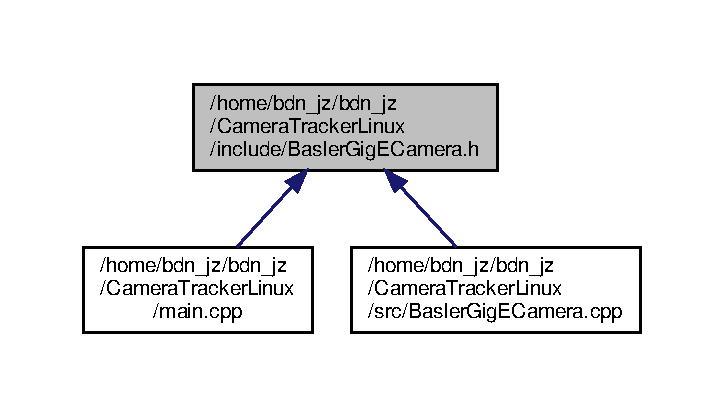
\includegraphics[width=350pt]{_basler_gig_e_camera_8h__dep__incl}
\end{center}
\end{figure}
\subsection*{Classes}
\begin{DoxyCompactItemize}
\item 
class \hyperlink{class_basler_gig_e_camera}{Basler\+Gig\+E\+Camera}
\begin{DoxyCompactList}\small\item\em Implementation of Basler GigE Cameras. \end{DoxyCompactList}\end{DoxyCompactItemize}


\subsection{Detailed Description}
Header file for the Basler GigE Camera class. 

File that contains the header of the Basler GigE Camera class. It relies on Pylon/\+Basler inlcudes but not on Qt. \begin{DoxyAuthor}{Author}
Benjamin Montavon 
\end{DoxyAuthor}
\begin{DoxyDate}{Date}
27.\+11.\+2015 
\end{DoxyDate}

\hypertarget{_chessboard_8h}{}\section{/home/bdn\+\_\+jz/bdn\+\_\+jz/\+Camera\+Tracker\+Linux/include/\+Chessboard.h File Reference}
\label{_chessboard_8h}\index{/home/bdn\+\_\+jz/bdn\+\_\+jz/\+Camera\+Tracker\+Linux/include/\+Chessboard.\+h@{/home/bdn\+\_\+jz/bdn\+\_\+jz/\+Camera\+Tracker\+Linux/include/\+Chessboard.\+h}}


This file contains the declaration of the \hyperlink{class_chessboard}{Chessboard} class.  


{\ttfamily \#include $<$opencv2/core.\+hpp$>$}\newline
{\ttfamily \#include $<$opencv2/opencv.\+hpp$>$}\newline
Include dependency graph for Chessboard.\+h\+:\nopagebreak
\begin{figure}[H]
\begin{center}
\leavevmode
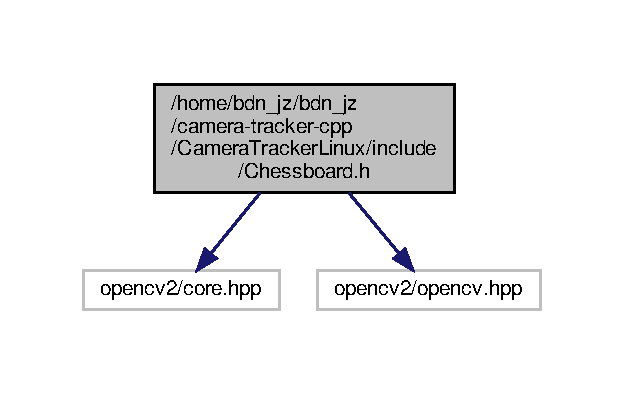
\includegraphics[width=300pt]{_chessboard_8h__incl}
\end{center}
\end{figure}
This graph shows which files directly or indirectly include this file\+:\nopagebreak
\begin{figure}[H]
\begin{center}
\leavevmode
\includegraphics[width=350pt]{_chessboard_8h__dep__incl}
\end{center}
\end{figure}
\subsection*{Classes}
\begin{DoxyCompactItemize}
\item 
class \hyperlink{class_chessboard}{Chessboard}
\begin{DoxyCompactList}\small\item\em Creation of chessboard. \end{DoxyCompactList}\end{DoxyCompactItemize}


\subsection{Detailed Description}
This file contains the declaration of the \hyperlink{class_chessboard}{Chessboard} class. 

\begin{DoxyAuthor}{Author}
Jiancong Zheng 
\end{DoxyAuthor}
\begin{DoxyDate}{Date}
2020-\/05-\/29 
\end{DoxyDate}

\hypertarget{_chessboard_detector_8h}{}\section{/home/bdn\+\_\+jz/bdn\+\_\+jz/camera-\/tracker-\/cpp/\+Camera\+Tracker\+Linux/include/\+Chessboard\+Detector.h File Reference}
\label{_chessboard_detector_8h}\index{/home/bdn\+\_\+jz/bdn\+\_\+jz/camera-\/tracker-\/cpp/\+Camera\+Tracker\+Linux/include/\+Chessboard\+Detector.\+h@{/home/bdn\+\_\+jz/bdn\+\_\+jz/camera-\/tracker-\/cpp/\+Camera\+Tracker\+Linux/include/\+Chessboard\+Detector.\+h}}


This file contains the declaration of the \hyperlink{class_chessboard_detector}{Chessboard\+Detector} class.  


{\ttfamily \#include \char`\"{}Chessboard.\+h\char`\"{}}\newline
Include dependency graph for Chessboard\+Detector.\+h\+:\nopagebreak
\begin{figure}[H]
\begin{center}
\leavevmode
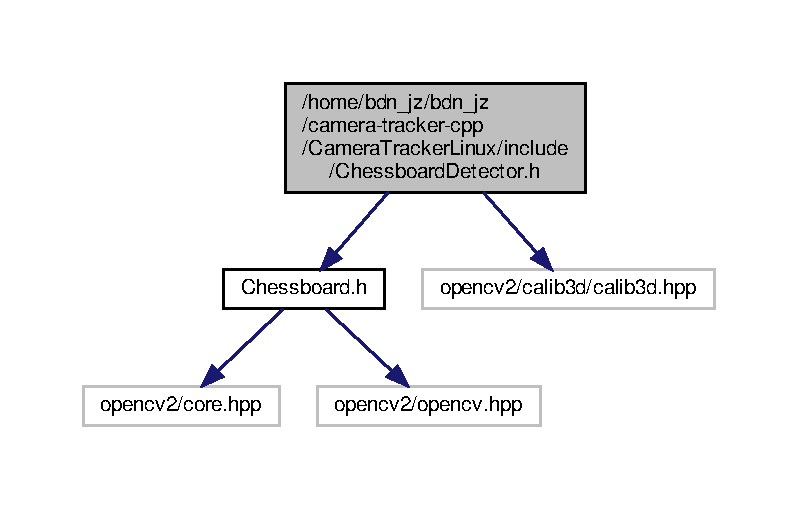
\includegraphics[width=300pt]{_chessboard_detector_8h__incl}
\end{center}
\end{figure}
This graph shows which files directly or indirectly include this file\+:
\nopagebreak
\begin{figure}[H]
\begin{center}
\leavevmode
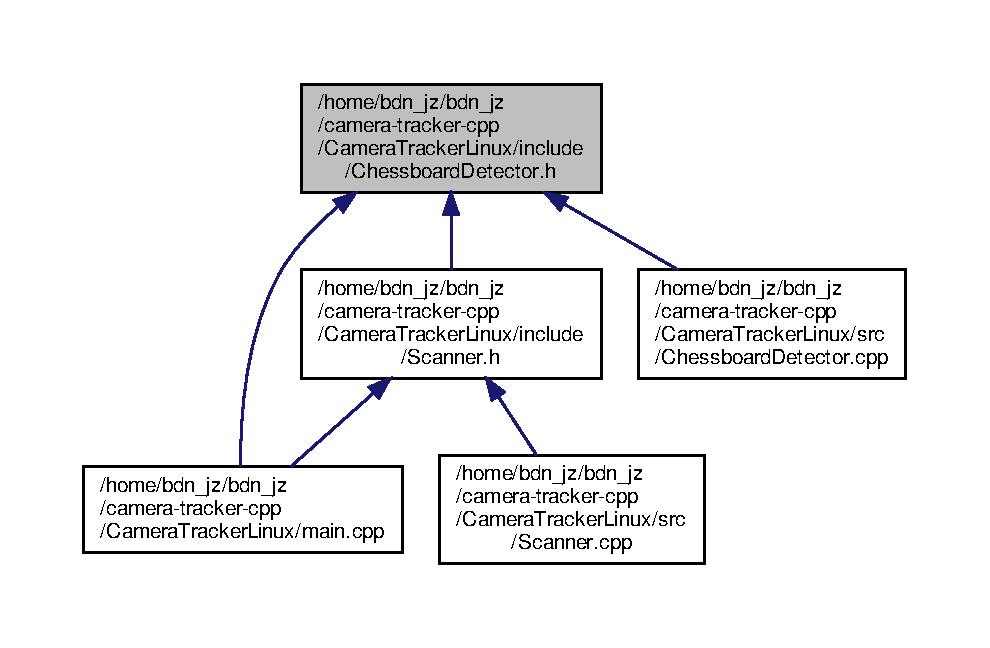
\includegraphics[width=350pt]{_chessboard_detector_8h__dep__incl}
\end{center}
\end{figure}
\subsection*{Classes}
\begin{DoxyCompactItemize}
\item 
struct \hyperlink{struct_find_corners_result}{Find\+Corners\+Result}
\begin{DoxyCompactList}\small\item\em Structure that contains the result of corner detection. \end{DoxyCompactList}\item 
struct \hyperlink{struct_perspective_result}{Perspective\+Result}
\begin{DoxyCompactList}\small\item\em Structure that contains the result of perspective transformation. \end{DoxyCompactList}\item 
struct \hyperlink{struct_chessboard_detector_result}{Chessboard\+Detector\+Result}
\begin{DoxyCompactList}\small\item\em Structure that contains the result of chessboard detection. \end{DoxyCompactList}\item 
class \hyperlink{class_chessboard_detector}{Chessboard\+Detector}
\begin{DoxyCompactList}\small\item\em Implementation of chessboard detection. \end{DoxyCompactList}\end{DoxyCompactItemize}
\subsection*{Typedefs}
\begin{DoxyCompactItemize}
\item 
typedef struct \hyperlink{struct_find_corners_result}{Find\+Corners\+Result} \hyperlink{_chessboard_detector_8h_aa8575bc4d17dcd5e64805de2349ef6de}{Find\+Corners\+Result}
\item 
typedef struct \hyperlink{struct_perspective_result}{Perspective\+Result} \hyperlink{_chessboard_detector_8h_aa5637be70ec0c07efb07d39f3cc8cd6e}{Perspective\+Result}
\item 
typedef struct \hyperlink{struct_chessboard_detector_result}{Chessboard\+Detector\+Result} \hyperlink{_chessboard_detector_8h_aea0f62d1c5d2fab51fe9b4c8516a5242}{Chessboard\+Detector\+Result}
\end{DoxyCompactItemize}


\subsection{Detailed Description}
This file contains the declaration of the \hyperlink{class_chessboard_detector}{Chessboard\+Detector} class. 

\begin{DoxyAuthor}{Author}
Jiancong Zheng 
\end{DoxyAuthor}
\begin{DoxyDate}{Date}
2020-\/05-\/29 
\end{DoxyDate}


\subsection{Typedef Documentation}
\mbox{\Hypertarget{_chessboard_detector_8h_aea0f62d1c5d2fab51fe9b4c8516a5242}\label{_chessboard_detector_8h_aea0f62d1c5d2fab51fe9b4c8516a5242}} 
\index{Chessboard\+Detector.\+h@{Chessboard\+Detector.\+h}!Chessboard\+Detector\+Result@{Chessboard\+Detector\+Result}}
\index{Chessboard\+Detector\+Result@{Chessboard\+Detector\+Result}!Chessboard\+Detector.\+h@{Chessboard\+Detector.\+h}}
\subsubsection{\texorpdfstring{Chessboard\+Detector\+Result}{ChessboardDetectorResult}}
{\footnotesize\ttfamily typedef struct \hyperlink{struct_chessboard_detector_result}{Chessboard\+Detector\+Result}  \hyperlink{struct_chessboard_detector_result}{Chessboard\+Detector\+Result}}

\mbox{\Hypertarget{_chessboard_detector_8h_aa8575bc4d17dcd5e64805de2349ef6de}\label{_chessboard_detector_8h_aa8575bc4d17dcd5e64805de2349ef6de}} 
\index{Chessboard\+Detector.\+h@{Chessboard\+Detector.\+h}!Find\+Corners\+Result@{Find\+Corners\+Result}}
\index{Find\+Corners\+Result@{Find\+Corners\+Result}!Chessboard\+Detector.\+h@{Chessboard\+Detector.\+h}}
\subsubsection{\texorpdfstring{Find\+Corners\+Result}{FindCornersResult}}
{\footnotesize\ttfamily typedef struct \hyperlink{struct_find_corners_result}{Find\+Corners\+Result}  \hyperlink{struct_find_corners_result}{Find\+Corners\+Result}}

\mbox{\Hypertarget{_chessboard_detector_8h_aa5637be70ec0c07efb07d39f3cc8cd6e}\label{_chessboard_detector_8h_aa5637be70ec0c07efb07d39f3cc8cd6e}} 
\index{Chessboard\+Detector.\+h@{Chessboard\+Detector.\+h}!Perspective\+Result@{Perspective\+Result}}
\index{Perspective\+Result@{Perspective\+Result}!Chessboard\+Detector.\+h@{Chessboard\+Detector.\+h}}
\subsubsection{\texorpdfstring{Perspective\+Result}{PerspectiveResult}}
{\footnotesize\ttfamily typedef struct \hyperlink{struct_perspective_result}{Perspective\+Result}  \hyperlink{struct_perspective_result}{Perspective\+Result}}


\hypertarget{_conex_8h}{}\section{/home/bdn\+\_\+jz/bdn\+\_\+jz/camera-\/tracker-\/cpp/\+Camera\+Tracker\+Linux/include/\+Conex.h File Reference}
\label{_conex_8h}\index{/home/bdn\+\_\+jz/bdn\+\_\+jz/camera-\/tracker-\/cpp/\+Camera\+Tracker\+Linux/include/\+Conex.\+h@{/home/bdn\+\_\+jz/bdn\+\_\+jz/camera-\/tracker-\/cpp/\+Camera\+Tracker\+Linux/include/\+Conex.\+h}}
{\ttfamily \#include $<$string$>$}\newline
{\ttfamily \#include $<$cstring$>$}\newline
Include dependency graph for Conex.\+h\+:
\nopagebreak
\begin{figure}[H]
\begin{center}
\leavevmode
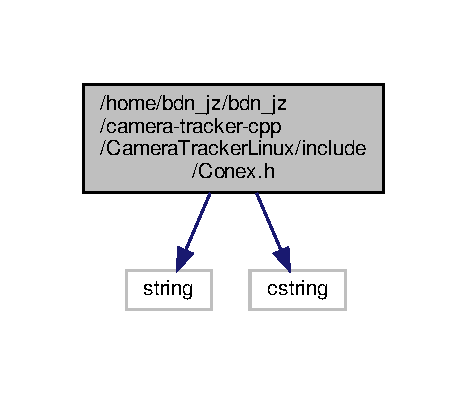
\includegraphics[width=224pt]{_conex_8h__incl}
\end{center}
\end{figure}
This graph shows which files directly or indirectly include this file\+:
\nopagebreak
\begin{figure}[H]
\begin{center}
\leavevmode
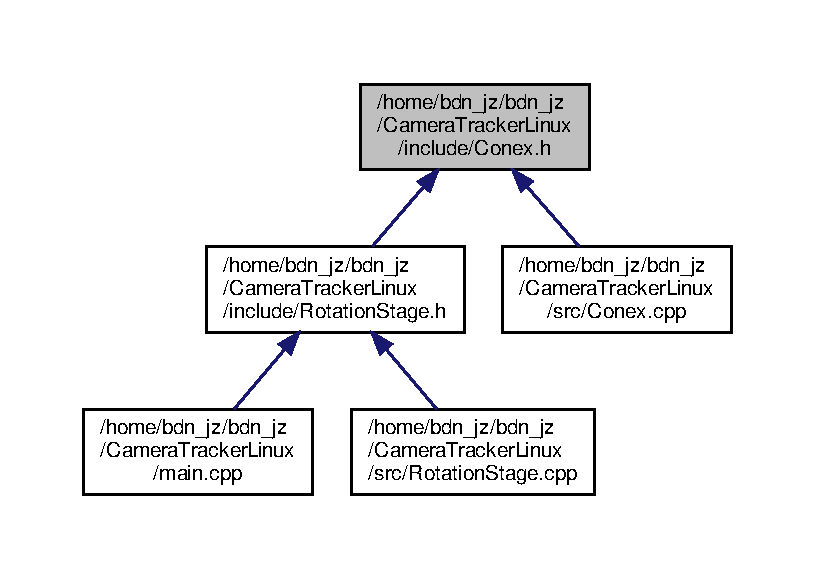
\includegraphics[width=350pt]{_conex_8h__dep__incl}
\end{center}
\end{figure}
\subsection*{Namespaces}
\begin{DoxyCompactItemize}
\item 
 \hyperlink{namespaceconex}{conex}
\end{DoxyCompactItemize}
\subsection*{Functions}
\begin{DoxyCompactItemize}
\item 
std\+::string \hyperlink{namespaceconex_a9ccf7065a08f5cb5c21c45efcb0c76db}{conex\+::get\+Acceleration} (int address\+Value)
\item 
std\+::string \hyperlink{namespaceconex_ae90d099ece6fb06e8eeb4ab3ad5df2bb}{conex\+::set\+Acceleration} (int address\+Value, float acceleration\+Value)
\item 
std\+::string \hyperlink{namespaceconex_a8c9d7fa13308de3bfa68ea372986d490}{conex\+::get\+Backlash\+Compensation} (int address\+Value)
\item 
std\+::string \hyperlink{namespaceconex_a8668932baaa1ff47f4bf37d6dabb1c42}{conex\+::set\+Backlash\+Compensation} (int address\+Value, float backlash\+Value)
\item 
std\+::string \hyperlink{namespaceconex_a44852cd57a643f1a70ffff0ba772b28b}{conex\+::get\+Hysteresis\+Compensation} (int address\+Value)
\item 
std\+::string \hyperlink{namespaceconex_a3a057c09b112f734431cb331669bc46b}{conex\+::set\+Hysteresis\+Compensation} (int address\+Value, float hysteresis\+Value)
\item 
std\+::string \hyperlink{namespaceconex_a0588a5e5f42da8cb5041900bbfba4243}{conex\+::get\+Driver\+Voltage} (int address\+Value)
\item 
std\+::string \hyperlink{namespaceconex_a07def2519839ea99940a654201ff40b9}{conex\+::set\+Driver\+Voltage} (int address\+Value, float driver\+Voltage\+Value)
\item 
std\+::string \hyperlink{namespaceconex_acaa2df03ff5ad416b1ed256995a40966}{conex\+::get\+Low\+Pass\+Filter\+Cut\+Off\+Frequency} (int address\+Value)
\item 
std\+::string \hyperlink{namespaceconex_a32f3870ece6ee316eff312c20fe069d3}{conex\+::set\+Low\+Pass\+Filter\+Cut\+Off\+Frequency} (int address\+Value, float cut\+Off\+Value)
\item 
std\+::string \hyperlink{namespaceconex_a05d5f0585af94bb38ccf8037d86768e5}{conex\+::get\+Following\+Error\+Limit} (int address\+Value)
\item 
std\+::string \hyperlink{namespaceconex_aecd28d691655d6fa73f28b2dd5922f8e}{conex\+::set\+Following\+Error\+Limit} (int address\+Value, float error\+Limit\+Value)
\item 
std\+::string \hyperlink{namespaceconex_afaa116b8274daffbd23139bb930596f9}{conex\+::get\+Friction\+Compensation} (int address\+Value)
\item 
std\+::string \hyperlink{namespaceconex_a45b737635000384b926ab6e2bd829865}{conex\+::set\+Friction\+Compensation} (int address\+Value, float friction\+Compensation\+Value)
\item 
std\+::string \hyperlink{namespaceconex_ad1b0c2c8ee173f299589772d4c2fd3b2}{conex\+::get\+Home\+Search\+Type} (int address\+Value)
\item 
std\+::string \hyperlink{namespaceconex_a2b7cd3e7462a4a8f2ba9e48ea5b5c450}{conex\+::set\+Home\+Search\+Type} (int address\+Value, int home\+Type\+Value)
\item 
std\+::string \hyperlink{namespaceconex_ad9475bdc92877f316a2e3db9ff0e8fb1}{conex\+::get\+Stage\+Identifier} (int address\+Value)
\item 
std\+::string \hyperlink{namespaceconex_a81886be7ef4e25e26a4a222d4716ea7f}{conex\+::set\+Stage\+Identifier} (int address\+Value, float model\+Number\+Value)
\item 
std\+::string \hyperlink{namespaceconex_acef19de1c3d630503736cf1bf20d4dbc}{conex\+::get\+Jerk\+Time} (int address\+Value)
\item 
std\+::string \hyperlink{namespaceconex_aa3f88891fb93e706d4be157b584a7f42}{conex\+::set\+Jerk\+Time} (int address\+Value, float jerk\+Time\+Value)
\item 
std\+::string \hyperlink{namespaceconex_a30cba542f0ebd8eea74032431fb29d21}{conex\+::get\+Derivative\+Gain} (int address\+Value)
\item 
std\+::string \hyperlink{namespaceconex_aa25149260c978531ca8f139da8b968b8}{conex\+::set\+Derivative\+Gain} (int address\+Value, float derivative\+Gain\+Value)
\item 
std\+::string \hyperlink{namespaceconex_ad08578dd23c3b65f2d73405ca35774ad}{conex\+::get\+Integral\+Gain} (int address\+Value)
\item 
std\+::string \hyperlink{namespaceconex_af806b975f4f1ce8ee3e83ce660f72593}{conex\+::set\+Integral\+Gain} (int address\+Value, float integral\+Gain\+Value)
\item 
std\+::string \hyperlink{namespaceconex_a0ed457be041ec821472eb60ef3f7768d}{conex\+::get\+Proportional\+Gain} (int address\+Value)
\item 
std\+::string \hyperlink{namespaceconex_a852e0fb570af45c7d523f94a2b81b84b}{conex\+::set\+Proportional\+Gain} (int address\+Value, float proportional\+Gain\+Value)
\item 
std\+::string \hyperlink{namespaceconex_aee916cc8cb9915577fc989826496fe6e}{conex\+::get\+Velocity\+Feed\+Forward} (int address\+Value)
\item 
std\+::string \hyperlink{namespaceconex_a5bcb38c3b971ccf0f2c03794ae16798c}{conex\+::set\+Velocity\+Feed\+Forward} (int address\+Value, float velocity\+Feed\+Forward\+Value)
\item 
std\+::string \hyperlink{namespaceconex_aa030f5f6f8e7d9de0c53bc783fd3b40a}{conex\+::get\+Disable\+State} (int address\+Value)
\item 
std\+::string \hyperlink{namespaceconex_a379241e6a2dafd2c5378ff9029a2afbb}{conex\+::disable\+State} (int address\+Value, bool command\+Value)
\item 
std\+::string \hyperlink{namespaceconex_a9bf3d6adb4fd4d48f95b2c27169ef773}{conex\+::get\+Home\+Search\+Velocity} (int address\+Value)
\item 
std\+::string \hyperlink{namespaceconex_ae0d284374b70f666fa8cad9bb3c81aa4}{conex\+::set\+Home\+Search\+Velocity} (int address\+Value, float velocity\+Value)
\item 
std\+::string \hyperlink{namespaceconex_a31e52a12a8f66df0c10a49931f7fce47}{conex\+::execute\+Home\+Search} (int address\+Value)
\item 
std\+::string \hyperlink{namespaceconex_a5652c22cdfb236799111449461eb88f5}{conex\+::get\+Home\+Search\+Time\+Out} (int address\+Value)
\item 
std\+::string \hyperlink{namespaceconex_a55f14dbf89cbe71b6d0934eef1a97d1b}{conex\+::set\+Home\+Search\+Time\+Out} (int address\+Value, float time\+Out\+Value)
\item 
std\+::string \hyperlink{namespaceconex_ae52a8731032ef6b65b942aa0573d81cc}{conex\+::move\+Absolute} (int address\+Value, float target\+Position\+Value)
\item 
std\+::string \hyperlink{namespaceconex_a6728914e77941e2fb4483b6721785ffb}{conex\+::move\+Relative} (int address\+Value, float displacement\+Value)
\item 
std\+::string \hyperlink{namespaceconex_aab2d3f712ba59df6e3001ea727d3c514}{conex\+::get\+Motion\+Time\+For\+Relative\+Move} (int address\+Value, float displacement\+Value)
\item 
std\+::string \hyperlink{namespaceconex_aa9f0011a56576d7e9382d9d7d211e946}{conex\+::configuration\+State} (int address\+Value, bool command\+Value)
\item 
std\+::string \hyperlink{namespaceconex_a4d69b5890ba99a072d3a3ef67f26047a}{conex\+::get\+Peak\+Current\+Limit} (int address\+Value)
\item 
std\+::string \hyperlink{namespaceconex_ad4e9c3f1429c4d356c4814c816b1ce42}{conex\+::set\+Peak\+Current\+Limit} (int address\+Value, float limit\+Value)
\item 
std\+::string \hyperlink{namespaceconex_a7f0202ac44e29e633656eac06ca43cd0}{conex\+::get\+R\+M\+S\+Current\+Limit} (int address\+Value)
\item 
std\+::string \hyperlink{namespaceconex_a3552f23ef324fc207a4b8ea8ca79d63c}{conex\+::set\+R\+M\+S\+Current\+Limit} (int address\+Value, float limit\+Value)
\item 
std\+::string \hyperlink{namespaceconex_a7c219ac12ae0d8c2385cbf3ef5aa2ed2}{conex\+::get\+R\+M\+S\+Averaging\+Time} (int address\+Value)
\item 
std\+::string \hyperlink{namespaceconex_a4db096ebf48bf2512a51c6f16f6d05a5}{conex\+::set\+R\+M\+S\+Averaging\+Time} (int address\+Value, float time\+Value)
\item 
std\+::string \hyperlink{namespaceconex_ac817039b6d386eae2ff9b288bee8c8f6}{conex\+::reset\+Controller} (int address\+Value)
\item 
std\+::string \hyperlink{namespaceconex_a4dd4ee5bd3729fc3cbf6e6f70f141baf}{conex\+::reset\+Controller\+Address} ()
\item 
std\+::string \hyperlink{namespaceconex_a50aafea583b1e9883f5c9da70f84e572}{conex\+::get\+Control\+Loop\+State} (int address\+Value)
\item 
std\+::string \hyperlink{namespaceconex_a617d632120418b5c8f501221c4b3c4e7}{conex\+::set\+Control\+Loop\+State} (int address\+Value, bool state\+Value)
\item 
std\+::string \hyperlink{namespaceconex_a5fe4df9385c4ac7842eee6c04fa6bda6}{conex\+::configure\+Simultaneous\+Started\+Move} (int address\+Value, float target\+Position\+Value)
\item 
std\+::string \hyperlink{namespaceconex_a2502bb0dfe401313b2505e560b41c8d5}{conex\+::execute\+Simultaneous\+Started\+Move} ()
\item 
std\+::string \hyperlink{namespaceconex_a66d5bce36b76f68906f18e8a553b07ea}{conex\+::get\+Simultaneous\+Configuration} (int address\+Value)
\item 
std\+::string \hyperlink{namespaceconex_a90e63f39f299603adfbab034098ae702}{conex\+::get\+Negative\+Software\+Limit} (int address\+Value)
\item 
std\+::string \hyperlink{namespaceconex_a70c1cfd0edc011bcf941ed9c4a63efe2}{conex\+::set\+Negative\+Software\+Limit} (int address\+Value, float Limit\+Value)
\item 
std\+::string \hyperlink{namespaceconex_ac78edbc8a18860189cd3963fb2b543f2}{conex\+::get\+Positive\+Software\+Limit} (int address\+Value)
\item 
std\+::string \hyperlink{namespaceconex_a786f1251f31ef6a30a042ac4fdbfb815}{conex\+::set\+Positive\+Software\+Limit} (int address\+Value, float Limit\+Value)
\item 
std\+::string \hyperlink{namespaceconex_aa908bd9ff7a78d0b2bd7bcbe2ef7080c}{conex\+::stop\+Motion} (int address\+Value)
\item 
std\+::string \hyperlink{namespaceconex_a8614267e3ba2e2c44b44bcd30bbb84b0}{conex\+::get\+Encoder\+Increment\+Value} (int address\+Value)
\item 
std\+::string \hyperlink{namespaceconex_a51a2f94e8cb024ecdc120c713dd19c7c}{conex\+::set\+Encoder\+Increment\+Value} (int address\+Value, float increment\+Value)
\item 
std\+::string \hyperlink{namespaceconex_a09ba026f23e2caeb631a18230bcd8b45}{conex\+::get\+Command\+Error\+String} (int address\+Value, char error)
\item 
std\+::string \hyperlink{namespaceconex_a6a993799643f4e7a19f0da530e03213e}{conex\+::get\+Last\+Command\+Error} (int address\+Value)
\item 
std\+::string \hyperlink{namespaceconex_a785c9ad7e52441aef38faeccf75c1e5e}{conex\+::get\+Set\+Point\+Position} (int address\+Value)
\item 
std\+::string \hyperlink{namespaceconex_a231ad931cd8782bcfd30f4b60ef2e3d8}{conex\+::tracking\+Mode} (int address\+Value, bool mode\+Value)
\item 
std\+::string \hyperlink{namespaceconex_abc96926292153eb7b8268a340eb140fc}{conex\+::get\+Current\+Postion} (int address\+Value)
\item 
std\+::string \hyperlink{namespaceconex_ab160c5ab9d6870ec2fdf198fede98ebd}{conex\+::get\+Postioner\+Error\+And\+Controller\+State} (int address\+Value)
\item 
std\+::string \hyperlink{namespaceconex_ab53c181f980eccedaa79f3b0154755df}{conex\+::get\+Velocity} (int address\+Value)
\item 
std\+::string \hyperlink{namespaceconex_aa970ffa1a5a264c97b5e821e1dedf0f0}{conex\+::set\+Velocity} (int address\+Value, float velocity\+Value)
\item 
std\+::string \hyperlink{namespaceconex_a0eb1fa3646288f0387cb303f0d8f71df}{conex\+::get\+Controller\+Revision\+Information} (int address\+Value)
\item 
std\+::string \hyperlink{namespaceconex_a7480495275a9236b221d635dd5bc08f8}{conex\+::get\+All\+Configuration\+Parameters} (int address\+Value)
\end{DoxyCompactItemize}

\hypertarget{constants_8h}{}\section{/home/jc/\+H\+I\+W\+I/camera-\/tracker-\/cpp/\+Camera\+Tracker\+Linux/include/constants.h File Reference}
\label{constants_8h}\index{/home/jc/\+H\+I\+W\+I/camera-\/tracker-\/cpp/\+Camera\+Tracker\+Linux/include/constants.\+h@{/home/jc/\+H\+I\+W\+I/camera-\/tracker-\/cpp/\+Camera\+Tracker\+Linux/include/constants.\+h}}


header for constant definitions.  


{\ttfamily \#include $<$opencv2/imgproc/imgproc.\+hpp$>$}\\*
Include dependency graph for constants.\+h\+:
% FIG 0
This graph shows which files directly or indirectly include this file\+:
% FIG 1
\subsection*{Macros}
\begin{DoxyCompactItemize}
\item 
\#define \hyperlink{constants_8h_a598a3330b3c21701223ee0ca14316eca}{PI}~3.\+14159265359
\begin{DoxyCompactList}\small\item\em pi, to avoid potential hassle with M\+\_\+\+PI \end{DoxyCompactList}\item 
\#define \hyperlink{constants_8h_a34a0a66cad070887d8b259e5e2fd0c67}{C\+V\+\_\+\+M\+O\+N\+O\+\_\+\+T\+Y\+PE}~C\+V\+\_\+16\+U\+C1
\begin{DoxyCompactList}\small\item\em Open\+CV type that will be used for monochroeme pictures, 16bit. \end{DoxyCompactList}\item 
\#define \hyperlink{constants_8h_a04143359709e6bc191324cdf9674b1e5}{C\+V\+\_\+\+C\+O\+L\+O\+R\+\_\+\+T\+Y\+PE}~C\+V\+\_\+16\+U\+C3
\begin{DoxyCompactList}\small\item\em Open\+CV colour type for displaying. \end{DoxyCompactList}\item 
\#define \hyperlink{constants_8h_ae7e5fc3d2bd8eb54b7c3bd9d2e81db31}{C\+V\+\_\+\+C\+P\+P\+\_\+\+T\+Y\+PE}~unsigned short
\begin{DoxyCompactList}\small\item\em internal data type that the open\+CV matrices use \end{DoxyCompactList}\item 
\#define \hyperlink{constants_8h_aa97b7c8af312feae18c3cb3daff56e03}{C\+V\+\_\+8\+\_\+\+T\+Y\+PE}~C\+V\+\_\+8\+U\+C1
\begin{DoxyCompactList}\small\item\em open\+CV data type for 8 bit matrices \end{DoxyCompactList}\item 
\#define \hyperlink{constants_8h_a0007c154f7281b17ecacda4af3fa5b13}{C\+V\+\_\+\+C\+P\+P\+\_\+8\+\_\+\+T\+Y\+PE}~unsigned char
\begin{DoxyCompactList}\small\item\em internal data type for 8 bit matrices \end{DoxyCompactList}\item 
\#define \hyperlink{constants_8h_a0e0900848f313188778907d811e612b9}{C\+V\+\_\+\+M\+A\+X\+\_\+\+V\+A\+L\+UE}~65535
\begin{DoxyCompactList}\small\item\em Maximum int value of 16 bit. \end{DoxyCompactList}\item 
\#define \hyperlink{constants_8h_a8282ccd73e76b7526e5ffc742667767a}{C\+V\+\_\+\+U\+P\+S\+C\+A\+L\+E\+\_\+12\+\_\+16}~16
\begin{DoxyCompactList}\small\item\em upscaling factor for 12 bit data \end{DoxyCompactList}\item 
\#define \hyperlink{constants_8h_a1f0468e0c9de8c0fd38d0d3ac10c2db0}{C\+V\+\_\+\+D\+O\+W\+N\+S\+C\+A\+L\+E\+\_\+12\+\_\+8}~1/double(16)
\begin{DoxyCompactList}\small\item\em downscaling factor for 12 bit data \end{DoxyCompactList}\item 
\#define \hyperlink{constants_8h_a8d5bca0308ac32963ea4f97f578baad4}{C\+V\+\_\+\+U\+P\+S\+C\+A\+L\+E\+\_\+8\+\_\+16}~256
\begin{DoxyCompactList}\small\item\em upscaling factor for 8 bit data \end{DoxyCompactList}\item 
\#define \hyperlink{constants_8h_a75c66eb5e918841eaf51925aae253c1e}{R\+W\+T\+H\+\_\+\+B\+L\+U\+E\+\_\+16}~C\+V\+\_\+\+R\+GB(0, 84$\ast$\hyperlink{constants_8h_a8d5bca0308ac32963ea4f97f578baad4}{C\+V\+\_\+\+U\+P\+S\+C\+A\+L\+E\+\_\+8\+\_\+16}, 159$\ast$\hyperlink{constants_8h_a8d5bca0308ac32963ea4f97f578baad4}{C\+V\+\_\+\+U\+P\+S\+C\+A\+L\+E\+\_\+8\+\_\+16})
\begin{DoxyCompactList}\small\item\em 16bit R\+W\+TH Blue corporate color definition \end{DoxyCompactList}\item 
\#define \hyperlink{constants_8h_ad4392fb13a4c86486a71cc4f83636468}{R\+W\+T\+H\+\_\+\+R\+E\+D\+\_\+16}~C\+V\+\_\+\+R\+GB(204$\ast$\hyperlink{constants_8h_a8d5bca0308ac32963ea4f97f578baad4}{C\+V\+\_\+\+U\+P\+S\+C\+A\+L\+E\+\_\+8\+\_\+16}, 7$\ast$\hyperlink{constants_8h_a8d5bca0308ac32963ea4f97f578baad4}{C\+V\+\_\+\+U\+P\+S\+C\+A\+L\+E\+\_\+8\+\_\+16}, 30$\ast$\hyperlink{constants_8h_a8d5bca0308ac32963ea4f97f578baad4}{C\+V\+\_\+\+U\+P\+S\+C\+A\+L\+E\+\_\+8\+\_\+16})
\begin{DoxyCompactList}\small\item\em 16bit R\+W\+TH Red corporate color definition \end{DoxyCompactList}\item 
\#define \hyperlink{constants_8h_a8af0c73884cd609b9cfc7495f70807b5}{M\+U\+T\+E\+X\+\_\+\+T\+I\+M\+E\+O\+UT}~1000
\begin{DoxyCompactList}\small\item\em default timeout for mutex trylock in ms \end{DoxyCompactList}\item 
\#define \hyperlink{constants_8h_a6e3b0a42e7726aba5267a3f74954ff4a}{I\+D\+S\+\_\+\+T\+I\+M\+E\+O\+UT}~10000
\begin{DoxyCompactList}\small\item\em response wait time for I\+D\+S3010 actions in ms \end{DoxyCompactList}\item 
\#define \hyperlink{constants_8h_a8f12c2088fc2f1895a328f0fcf78a65e}{I\+D\+S\+\_\+\+D\+E\+F\+A\+U\+L\+T\+\_\+\+R\+E\+F\+R\+E\+SH}~100
\begin{DoxyCompactList}\small\item\em default refresh rate for displacement data in ms \end{DoxyCompactList}\item 
\#define \hyperlink{constants_8h_a739a2f8edf4dab990c2ea1ee5488a158}{E\+C\+U\+\_\+\+D\+E\+F\+A\+U\+L\+T\+\_\+\+R\+E\+F\+R\+E\+SH}~10000
\begin{DoxyCompactList}\small\item\em default refresh rate for E\+CU data in ms \end{DoxyCompactList}\item 
\#define \hyperlink{constants_8h_aae46594e11eab2b349f59f2427bae4b5}{I\+D\+S\+\_\+\+D\+E\+F\+A\+U\+L\+T\+\_\+\+A\+V\+E\+R\+A\+GE}~8
\begin{DoxyCompactList}\small\item\em default I\+DS average setting \end{DoxyCompactList}\item 
\#define \hyperlink{constants_8h_ad1d4e1add87a3824892fcdd912313f6d}{B\+A\+S\+L\+E\+R\+\_\+\+D\+E\+F\+A\+U\+L\+T\+\_\+\+P\+I\+T\+CH}~0.\+00167
\begin{DoxyCompactList}\small\item\em default pitch value to set for Basler cameras \end{DoxyCompactList}\item 
\#define \hyperlink{constants_8h_ac357928f4dcf1c65416dce5f6b8459af}{V\+I\+R\+T\+U\+A\+L\+\_\+\+D\+E\+F\+A\+U\+L\+T\+\_\+\+P\+I\+T\+CH}~1.\+0
\begin{DoxyCompactList}\small\item\em default pitch value for virtual cameras \end{DoxyCompactList}\item 
\#define \hyperlink{constants_8h_a172aa202ec9ae82f4104bd8867571bd2}{V\+I\+R\+T\+U\+A\+L\+\_\+\+F\+PS}~10
\begin{DoxyCompactList}\small\item\em theoretical frame rate of virtual cameras \end{DoxyCompactList}\item 
\#define \hyperlink{constants_8h_afffeeea9c511d12bf1c0583dcb622d2d}{B\+E\+E\+P\+\_\+\+F\+R\+E\+Q\+U\+E\+N\+CY}~880
\begin{DoxyCompactList}\small\item\em frequency to use for beeps in Hz \end{DoxyCompactList}\item 
\#define \hyperlink{constants_8h_a5fd7d449b655d9ceff4997dfaee50e18}{R\+E\+S\+U\+L\+T\+\_\+\+P\+R\+E\+C\+I\+S\+I\+ON}~6
\begin{DoxyCompactList}\small\item\em default digit display if format \end{DoxyCompactList}\item 
\#define \hyperlink{constants_8h_a6c7ea402893dffa8ab4020dc647b2245}{L\+A\+S\+E\+R\+\_\+\+E\+X\+P\+O\+S\+E\+\_\+\+I\+T\+E\+R\+A\+T\+I\+O\+NS}~50
\begin{DoxyCompactList}\small\item\em default limit before laser exposure is aborted \end{DoxyCompactList}\item 
\#define \hyperlink{constants_8h_aec3698fa38dbcb13be0976e53dae92c3}{M\+E\+A\+S\+U\+R\+E\+\_\+\+P\+E\+R\+F\+O\+R\+M\+A\+N\+C\+E\+\_\+\+B\+A\+R\+R\+I\+ER}~500
\begin{DoxyCompactList}\small\item\em security barrier between device measurements for low performance mode in ms \end{DoxyCompactList}\item 
\#define \hyperlink{constants_8h_a5193e4114ac09604221954b3ad7082d4}{P\+E\+\_\+\+D\+E\+F\+A\+U\+LT}~0x10101
\item 
\#define \hyperlink{constants_8h_ae6504fd9029194fe12b014580e8cadee}{P\+E\+\_\+\+S\+I\+N\+G\+LE}~0x10101
\item 
\#define \hyperlink{constants_8h_a383c24bbdaf58efea1a42d0613a6f40a}{P\+E\+\_\+\+S\+T\+E\+R\+EO}~0x10102
\item 
\#define \hyperlink{constants_8h_af7877d5baf4e2e56e33e8131ea4baf6b}{C\+D\+\_\+\+D\+E\+F\+A\+U\+LT}~0x10202
\item 
\#define \hyperlink{constants_8h_af2d9c506d3acbff804caeba40e94b7d9}{C\+D\+\_\+\+F\+E\+A\+T\+U\+RE}~0x10201
\item 
\#define \hyperlink{constants_8h_a2d0c40a1cc18d63608cd689e3ad35ca6}{C\+D\+\_\+\+M\+E\+TA}~0x10202
\item 
\#define \hyperlink{constants_8h_a5a33f0f7759d7133fbd4a976c51295d0}{C\+D\+\_\+\+T\+E\+M\+P\+L\+A\+TE}~0x10203
\item 
\#define \hyperlink{constants_8h_abe821f88bfb11667becdbee1e1b24d1d}{T\+M\+\_\+\+D\+E\+F\+A\+U\+LT}~0x20101
\item 
\#define \hyperlink{constants_8h_a53e908ab375fe7a1c7f8423e0dcbb43a}{T\+M\+\_\+\+C\+O\+RR}~0x20101
\item 
\#define \hyperlink{constants_8h_acf6f14d8154fe3b4ce092bf6d65ba37a}{T\+M\+\_\+\+C\+O\+EF}~0x20102
\item 
\#define \hyperlink{constants_8h_a17342c9bc959c61efd243a0865f0b672}{T\+M\+\_\+\+M\+S\+QD}~0x20103
\item 
\#define \hyperlink{constants_8h_a7736a4df685c629365fa2a6001a8b08b}{M\+A\+X\+\_\+\+I\+M\+A\+G\+E\+\_\+\+A\+X\+IS}~600
\begin{DoxyCompactList}\small\item\em maximal length of the longer image axis \end{DoxyCompactList}\item 
\#define \hyperlink{constants_8h_af3c82099d63a2d91d68bd62d954059c7}{M\+A\+X\+\_\+\+A\+N\+G\+LE}~10
\begin{DoxyCompactList}\small\item\em maximal allowed angle between the detected cable and the ideal position \end{DoxyCompactList}\item 
\#define \hyperlink{constants_8h_a549d41dcf9444ed7d6df1da3c73e7d16}{M\+I\+N\+\_\+\+D\+I\+S\+T\+A\+N\+CE}~20
\item 
\#define \hyperlink{constants_8h_ab0cfbe1ce4855ea05fc84dadf183414a}{C\+A\+N\+N\+Y\+\_\+\+M\+I\+N\+\_\+\+T\+H\+R\+E\+S\+H\+O\+LD}~50
\item 
\#define \hyperlink{constants_8h_a9f9ca7a9a0789cf570ab3f0772ccfd6f}{C\+A\+N\+N\+Y\+\_\+\+M\+A\+X\+\_\+\+T\+H\+R\+E\+S\+H\+O\+LD}~2 $\ast$ \hyperlink{constants_8h_ab0cfbe1ce4855ea05fc84dadf183414a}{C\+A\+N\+N\+Y\+\_\+\+M\+I\+N\+\_\+\+T\+H\+R\+E\+S\+H\+O\+LD}
\item 
\#define \hyperlink{constants_8h_aac018fc017489b79204fe23a3072ed97}{L\+E\+F\+T\+\_\+\+C\+AM}~\char`\"{}22176689\char`\"{}
\item 
\#define \hyperlink{constants_8h_a3fa25cff21013fb9d8993aadb27fe638}{T\+O\+P\+\_\+\+C\+AM}~\char`\"{}22176687\char`\"{}
\item 
\#define \hyperlink{constants_8h_a9d1726b216e8914a576e76c5aba9a144}{R\+I\+G\+H\+T\+\_\+\+C\+AM}~\char`\"{}22176686\char`\"{}
\item 
\#define \hyperlink{constants_8h_a2366d8e6e85d83991c14dca7561048b2}{L\+E\+F\+T\+\_\+\+C\+A\+L\+I\+B\+\_\+\+L\+OC}~\char`\"{}..\textbackslash{}assets\textbackslash{}calibration\+\_\+images\+\_\+labor\textbackslash{}left\+\_\+cam\char`\"{}
\item 
\#define \hyperlink{constants_8h_a10b46d0c4c42eff05c5e0db82aaf52d2}{T\+O\+P\+\_\+\+C\+A\+L\+I\+B\+\_\+\+L\+OC}~\char`\"{}..\textbackslash{}assets\textbackslash{}calibration\+\_\+images\+\_\+labor\textbackslash{}top\+\_\+cam\char`\"{}
\item 
\#define \hyperlink{constants_8h_a488c7f89c928ac0cd1cfaa085f1d1922}{R\+I\+G\+H\+T\+\_\+\+C\+A\+L\+I\+B\+\_\+\+L\+OC}~\char`\"{}..\textbackslash{}assets\textbackslash{}calibration\+\_\+images\+\_\+labor\textbackslash{}right\+\_\+cam\char`\"{}
\item 
\#define \hyperlink{constants_8h_ad72dbcf6d0153db1b8d8a58001feed83}{D\+E\+B\+UG}~2
\item 
\#define \hyperlink{constants_8h_a29779b3f0f58b3bd6a1baca88021c4df}{D\+O\+UT}(x)~if (\hyperlink{constants_8h_ad72dbcf6d0153db1b8d8a58001feed83}{D\+E\+B\+UG} $>$ 0) \{std\+::cout $<$$<$ x;\}
\item 
\#define \hyperlink{constants_8h_afe67f82eb9c5f9b21b8fda0638ed4874}{D\+S\+H\+OW}(x,  y,  z)~if (\hyperlink{constants_8h_ad72dbcf6d0153db1b8d8a58001feed83}{D\+E\+B\+UG} $>$ 1) \{utils\+::show\+Image(x, y, z);\}
\end{DoxyCompactItemize}
\subsection*{Enumerations}
\begin{DoxyCompactItemize}
\item 
enum \hyperlink{constants_8h_a6e920987695b1da6e2df4e41dc867e18}{Exposure\+Modes} \{ \hyperlink{constants_8h_a6e920987695b1da6e2df4e41dc867e18aeef9468d1b98bca652a04bf5063fd9d6}{A\+U\+TO}, 
\hyperlink{constants_8h_a6e920987695b1da6e2df4e41dc867e18a506e8dd29460ea318b68d035f679b01b}{M\+A\+N\+U\+AL}, 
\hyperlink{constants_8h_a6e920987695b1da6e2df4e41dc867e18a2e9dfa1d5da5e771b087db2ca9ed77f7}{L\+A\+S\+ER}
 \}
\item 
enum \hyperlink{constants_8h_ae9749bac8d6973b92725af092d0a76bc}{Exposure\+States} \{ \hyperlink{constants_8h_ae9749bac8d6973b92725af092d0a76bcafe29bdbfb6e2165eec29bf28af429856}{B\+AD}, 
\hyperlink{constants_8h_ae9749bac8d6973b92725af092d0a76bca8eb0135a04a7e7daf1ca4abf2c87832c}{G\+O\+OD}
 \}
\end{DoxyCompactItemize}


\subsection{Detailed Description}
header for constant definitions. 

Header file that contains useful constant definitions together in one place, avoiding value hardcoding \begin{DoxyAuthor}{Author}
Benjamin Montavon 
\end{DoxyAuthor}
\begin{DoxyDate}{Date}
27.\+11.\+2015 
\end{DoxyDate}


\subsection{Macro Definition Documentation}
\index{constants.\+h@{constants.\+h}!B\+A\+S\+L\+E\+R\+\_\+\+D\+E\+F\+A\+U\+L\+T\+\_\+\+P\+I\+T\+CH@{B\+A\+S\+L\+E\+R\+\_\+\+D\+E\+F\+A\+U\+L\+T\+\_\+\+P\+I\+T\+CH}}
\index{B\+A\+S\+L\+E\+R\+\_\+\+D\+E\+F\+A\+U\+L\+T\+\_\+\+P\+I\+T\+CH@{B\+A\+S\+L\+E\+R\+\_\+\+D\+E\+F\+A\+U\+L\+T\+\_\+\+P\+I\+T\+CH}!constants.\+h@{constants.\+h}}
\subsubsection[{\texorpdfstring{B\+A\+S\+L\+E\+R\+\_\+\+D\+E\+F\+A\+U\+L\+T\+\_\+\+P\+I\+T\+CH}{BASLER_DEFAULT_PITCH}}]{\setlength{\rightskip}{0pt plus 5cm}\#define B\+A\+S\+L\+E\+R\+\_\+\+D\+E\+F\+A\+U\+L\+T\+\_\+\+P\+I\+T\+CH~0.\+00167}\hypertarget{constants_8h_ad1d4e1add87a3824892fcdd912313f6d}{}\label{constants_8h_ad1d4e1add87a3824892fcdd912313f6d}


default pitch value to set for Basler cameras 

\index{constants.\+h@{constants.\+h}!B\+E\+E\+P\+\_\+\+F\+R\+E\+Q\+U\+E\+N\+CY@{B\+E\+E\+P\+\_\+\+F\+R\+E\+Q\+U\+E\+N\+CY}}
\index{B\+E\+E\+P\+\_\+\+F\+R\+E\+Q\+U\+E\+N\+CY@{B\+E\+E\+P\+\_\+\+F\+R\+E\+Q\+U\+E\+N\+CY}!constants.\+h@{constants.\+h}}
\subsubsection[{\texorpdfstring{B\+E\+E\+P\+\_\+\+F\+R\+E\+Q\+U\+E\+N\+CY}{BEEP_FREQUENCY}}]{\setlength{\rightskip}{0pt plus 5cm}\#define B\+E\+E\+P\+\_\+\+F\+R\+E\+Q\+U\+E\+N\+CY~880}\hypertarget{constants_8h_afffeeea9c511d12bf1c0583dcb622d2d}{}\label{constants_8h_afffeeea9c511d12bf1c0583dcb622d2d}


frequency to use for beeps in Hz 

\index{constants.\+h@{constants.\+h}!C\+A\+N\+N\+Y\+\_\+\+M\+A\+X\+\_\+\+T\+H\+R\+E\+S\+H\+O\+LD@{C\+A\+N\+N\+Y\+\_\+\+M\+A\+X\+\_\+\+T\+H\+R\+E\+S\+H\+O\+LD}}
\index{C\+A\+N\+N\+Y\+\_\+\+M\+A\+X\+\_\+\+T\+H\+R\+E\+S\+H\+O\+LD@{C\+A\+N\+N\+Y\+\_\+\+M\+A\+X\+\_\+\+T\+H\+R\+E\+S\+H\+O\+LD}!constants.\+h@{constants.\+h}}
\subsubsection[{\texorpdfstring{C\+A\+N\+N\+Y\+\_\+\+M\+A\+X\+\_\+\+T\+H\+R\+E\+S\+H\+O\+LD}{CANNY_MAX_THRESHOLD}}]{\setlength{\rightskip}{0pt plus 5cm}\#define C\+A\+N\+N\+Y\+\_\+\+M\+A\+X\+\_\+\+T\+H\+R\+E\+S\+H\+O\+LD~2 $\ast$ {\bf C\+A\+N\+N\+Y\+\_\+\+M\+I\+N\+\_\+\+T\+H\+R\+E\+S\+H\+O\+LD}}\hypertarget{constants_8h_a9f9ca7a9a0789cf570ab3f0772ccfd6f}{}\label{constants_8h_a9f9ca7a9a0789cf570ab3f0772ccfd6f}
\index{constants.\+h@{constants.\+h}!C\+A\+N\+N\+Y\+\_\+\+M\+I\+N\+\_\+\+T\+H\+R\+E\+S\+H\+O\+LD@{C\+A\+N\+N\+Y\+\_\+\+M\+I\+N\+\_\+\+T\+H\+R\+E\+S\+H\+O\+LD}}
\index{C\+A\+N\+N\+Y\+\_\+\+M\+I\+N\+\_\+\+T\+H\+R\+E\+S\+H\+O\+LD@{C\+A\+N\+N\+Y\+\_\+\+M\+I\+N\+\_\+\+T\+H\+R\+E\+S\+H\+O\+LD}!constants.\+h@{constants.\+h}}
\subsubsection[{\texorpdfstring{C\+A\+N\+N\+Y\+\_\+\+M\+I\+N\+\_\+\+T\+H\+R\+E\+S\+H\+O\+LD}{CANNY_MIN_THRESHOLD}}]{\setlength{\rightskip}{0pt plus 5cm}\#define C\+A\+N\+N\+Y\+\_\+\+M\+I\+N\+\_\+\+T\+H\+R\+E\+S\+H\+O\+LD~50}\hypertarget{constants_8h_ab0cfbe1ce4855ea05fc84dadf183414a}{}\label{constants_8h_ab0cfbe1ce4855ea05fc84dadf183414a}
\index{constants.\+h@{constants.\+h}!C\+D\+\_\+\+D\+E\+F\+A\+U\+LT@{C\+D\+\_\+\+D\+E\+F\+A\+U\+LT}}
\index{C\+D\+\_\+\+D\+E\+F\+A\+U\+LT@{C\+D\+\_\+\+D\+E\+F\+A\+U\+LT}!constants.\+h@{constants.\+h}}
\subsubsection[{\texorpdfstring{C\+D\+\_\+\+D\+E\+F\+A\+U\+LT}{CD_DEFAULT}}]{\setlength{\rightskip}{0pt plus 5cm}\#define C\+D\+\_\+\+D\+E\+F\+A\+U\+LT~0x10202}\hypertarget{constants_8h_af7877d5baf4e2e56e33e8131ea4baf6b}{}\label{constants_8h_af7877d5baf4e2e56e33e8131ea4baf6b}
\index{constants.\+h@{constants.\+h}!C\+D\+\_\+\+F\+E\+A\+T\+U\+RE@{C\+D\+\_\+\+F\+E\+A\+T\+U\+RE}}
\index{C\+D\+\_\+\+F\+E\+A\+T\+U\+RE@{C\+D\+\_\+\+F\+E\+A\+T\+U\+RE}!constants.\+h@{constants.\+h}}
\subsubsection[{\texorpdfstring{C\+D\+\_\+\+F\+E\+A\+T\+U\+RE}{CD_FEATURE}}]{\setlength{\rightskip}{0pt plus 5cm}\#define C\+D\+\_\+\+F\+E\+A\+T\+U\+RE~0x10201}\hypertarget{constants_8h_af2d9c506d3acbff804caeba40e94b7d9}{}\label{constants_8h_af2d9c506d3acbff804caeba40e94b7d9}
\index{constants.\+h@{constants.\+h}!C\+D\+\_\+\+M\+E\+TA@{C\+D\+\_\+\+M\+E\+TA}}
\index{C\+D\+\_\+\+M\+E\+TA@{C\+D\+\_\+\+M\+E\+TA}!constants.\+h@{constants.\+h}}
\subsubsection[{\texorpdfstring{C\+D\+\_\+\+M\+E\+TA}{CD_META}}]{\setlength{\rightskip}{0pt plus 5cm}\#define C\+D\+\_\+\+M\+E\+TA~0x10202}\hypertarget{constants_8h_a2d0c40a1cc18d63608cd689e3ad35ca6}{}\label{constants_8h_a2d0c40a1cc18d63608cd689e3ad35ca6}
\index{constants.\+h@{constants.\+h}!C\+D\+\_\+\+T\+E\+M\+P\+L\+A\+TE@{C\+D\+\_\+\+T\+E\+M\+P\+L\+A\+TE}}
\index{C\+D\+\_\+\+T\+E\+M\+P\+L\+A\+TE@{C\+D\+\_\+\+T\+E\+M\+P\+L\+A\+TE}!constants.\+h@{constants.\+h}}
\subsubsection[{\texorpdfstring{C\+D\+\_\+\+T\+E\+M\+P\+L\+A\+TE}{CD_TEMPLATE}}]{\setlength{\rightskip}{0pt plus 5cm}\#define C\+D\+\_\+\+T\+E\+M\+P\+L\+A\+TE~0x10203}\hypertarget{constants_8h_a5a33f0f7759d7133fbd4a976c51295d0}{}\label{constants_8h_a5a33f0f7759d7133fbd4a976c51295d0}
\index{constants.\+h@{constants.\+h}!C\+V\+\_\+8\+\_\+\+T\+Y\+PE@{C\+V\+\_\+8\+\_\+\+T\+Y\+PE}}
\index{C\+V\+\_\+8\+\_\+\+T\+Y\+PE@{C\+V\+\_\+8\+\_\+\+T\+Y\+PE}!constants.\+h@{constants.\+h}}
\subsubsection[{\texorpdfstring{C\+V\+\_\+8\+\_\+\+T\+Y\+PE}{CV_8_TYPE}}]{\setlength{\rightskip}{0pt plus 5cm}\#define C\+V\+\_\+8\+\_\+\+T\+Y\+PE~C\+V\+\_\+8\+U\+C1}\hypertarget{constants_8h_aa97b7c8af312feae18c3cb3daff56e03}{}\label{constants_8h_aa97b7c8af312feae18c3cb3daff56e03}


open\+CV data type for 8 bit matrices 

\index{constants.\+h@{constants.\+h}!C\+V\+\_\+\+C\+O\+L\+O\+R\+\_\+\+T\+Y\+PE@{C\+V\+\_\+\+C\+O\+L\+O\+R\+\_\+\+T\+Y\+PE}}
\index{C\+V\+\_\+\+C\+O\+L\+O\+R\+\_\+\+T\+Y\+PE@{C\+V\+\_\+\+C\+O\+L\+O\+R\+\_\+\+T\+Y\+PE}!constants.\+h@{constants.\+h}}
\subsubsection[{\texorpdfstring{C\+V\+\_\+\+C\+O\+L\+O\+R\+\_\+\+T\+Y\+PE}{CV_COLOR_TYPE}}]{\setlength{\rightskip}{0pt plus 5cm}\#define C\+V\+\_\+\+C\+O\+L\+O\+R\+\_\+\+T\+Y\+PE~C\+V\+\_\+16\+U\+C3}\hypertarget{constants_8h_a04143359709e6bc191324cdf9674b1e5}{}\label{constants_8h_a04143359709e6bc191324cdf9674b1e5}


Open\+CV colour type for displaying. 

\index{constants.\+h@{constants.\+h}!C\+V\+\_\+\+C\+P\+P\+\_\+8\+\_\+\+T\+Y\+PE@{C\+V\+\_\+\+C\+P\+P\+\_\+8\+\_\+\+T\+Y\+PE}}
\index{C\+V\+\_\+\+C\+P\+P\+\_\+8\+\_\+\+T\+Y\+PE@{C\+V\+\_\+\+C\+P\+P\+\_\+8\+\_\+\+T\+Y\+PE}!constants.\+h@{constants.\+h}}
\subsubsection[{\texorpdfstring{C\+V\+\_\+\+C\+P\+P\+\_\+8\+\_\+\+T\+Y\+PE}{CV_CPP_8_TYPE}}]{\setlength{\rightskip}{0pt plus 5cm}\#define C\+V\+\_\+\+C\+P\+P\+\_\+8\+\_\+\+T\+Y\+PE~unsigned char}\hypertarget{constants_8h_a0007c154f7281b17ecacda4af3fa5b13}{}\label{constants_8h_a0007c154f7281b17ecacda4af3fa5b13}


internal data type for 8 bit matrices 

\index{constants.\+h@{constants.\+h}!C\+V\+\_\+\+C\+P\+P\+\_\+\+T\+Y\+PE@{C\+V\+\_\+\+C\+P\+P\+\_\+\+T\+Y\+PE}}
\index{C\+V\+\_\+\+C\+P\+P\+\_\+\+T\+Y\+PE@{C\+V\+\_\+\+C\+P\+P\+\_\+\+T\+Y\+PE}!constants.\+h@{constants.\+h}}
\subsubsection[{\texorpdfstring{C\+V\+\_\+\+C\+P\+P\+\_\+\+T\+Y\+PE}{CV_CPP_TYPE}}]{\setlength{\rightskip}{0pt plus 5cm}\#define C\+V\+\_\+\+C\+P\+P\+\_\+\+T\+Y\+PE~unsigned short}\hypertarget{constants_8h_ae7e5fc3d2bd8eb54b7c3bd9d2e81db31}{}\label{constants_8h_ae7e5fc3d2bd8eb54b7c3bd9d2e81db31}


internal data type that the open\+CV matrices use 

\index{constants.\+h@{constants.\+h}!C\+V\+\_\+\+D\+O\+W\+N\+S\+C\+A\+L\+E\+\_\+12\+\_\+8@{C\+V\+\_\+\+D\+O\+W\+N\+S\+C\+A\+L\+E\+\_\+12\+\_\+8}}
\index{C\+V\+\_\+\+D\+O\+W\+N\+S\+C\+A\+L\+E\+\_\+12\+\_\+8@{C\+V\+\_\+\+D\+O\+W\+N\+S\+C\+A\+L\+E\+\_\+12\+\_\+8}!constants.\+h@{constants.\+h}}
\subsubsection[{\texorpdfstring{C\+V\+\_\+\+D\+O\+W\+N\+S\+C\+A\+L\+E\+\_\+12\+\_\+8}{CV_DOWNSCALE_12_8}}]{\setlength{\rightskip}{0pt plus 5cm}\#define C\+V\+\_\+\+D\+O\+W\+N\+S\+C\+A\+L\+E\+\_\+12\+\_\+8~1/double(16)}\hypertarget{constants_8h_a1f0468e0c9de8c0fd38d0d3ac10c2db0}{}\label{constants_8h_a1f0468e0c9de8c0fd38d0d3ac10c2db0}


downscaling factor for 12 bit data 

\index{constants.\+h@{constants.\+h}!C\+V\+\_\+\+M\+A\+X\+\_\+\+V\+A\+L\+UE@{C\+V\+\_\+\+M\+A\+X\+\_\+\+V\+A\+L\+UE}}
\index{C\+V\+\_\+\+M\+A\+X\+\_\+\+V\+A\+L\+UE@{C\+V\+\_\+\+M\+A\+X\+\_\+\+V\+A\+L\+UE}!constants.\+h@{constants.\+h}}
\subsubsection[{\texorpdfstring{C\+V\+\_\+\+M\+A\+X\+\_\+\+V\+A\+L\+UE}{CV_MAX_VALUE}}]{\setlength{\rightskip}{0pt plus 5cm}\#define C\+V\+\_\+\+M\+A\+X\+\_\+\+V\+A\+L\+UE~65535}\hypertarget{constants_8h_a0e0900848f313188778907d811e612b9}{}\label{constants_8h_a0e0900848f313188778907d811e612b9}


Maximum int value of 16 bit. 

\index{constants.\+h@{constants.\+h}!C\+V\+\_\+\+M\+O\+N\+O\+\_\+\+T\+Y\+PE@{C\+V\+\_\+\+M\+O\+N\+O\+\_\+\+T\+Y\+PE}}
\index{C\+V\+\_\+\+M\+O\+N\+O\+\_\+\+T\+Y\+PE@{C\+V\+\_\+\+M\+O\+N\+O\+\_\+\+T\+Y\+PE}!constants.\+h@{constants.\+h}}
\subsubsection[{\texorpdfstring{C\+V\+\_\+\+M\+O\+N\+O\+\_\+\+T\+Y\+PE}{CV_MONO_TYPE}}]{\setlength{\rightskip}{0pt plus 5cm}\#define C\+V\+\_\+\+M\+O\+N\+O\+\_\+\+T\+Y\+PE~C\+V\+\_\+16\+U\+C1}\hypertarget{constants_8h_a34a0a66cad070887d8b259e5e2fd0c67}{}\label{constants_8h_a34a0a66cad070887d8b259e5e2fd0c67}


Open\+CV type that will be used for monochroeme pictures, 16bit. 

\index{constants.\+h@{constants.\+h}!C\+V\+\_\+\+U\+P\+S\+C\+A\+L\+E\+\_\+12\+\_\+16@{C\+V\+\_\+\+U\+P\+S\+C\+A\+L\+E\+\_\+12\+\_\+16}}
\index{C\+V\+\_\+\+U\+P\+S\+C\+A\+L\+E\+\_\+12\+\_\+16@{C\+V\+\_\+\+U\+P\+S\+C\+A\+L\+E\+\_\+12\+\_\+16}!constants.\+h@{constants.\+h}}
\subsubsection[{\texorpdfstring{C\+V\+\_\+\+U\+P\+S\+C\+A\+L\+E\+\_\+12\+\_\+16}{CV_UPSCALE_12_16}}]{\setlength{\rightskip}{0pt plus 5cm}\#define C\+V\+\_\+\+U\+P\+S\+C\+A\+L\+E\+\_\+12\+\_\+16~16}\hypertarget{constants_8h_a8282ccd73e76b7526e5ffc742667767a}{}\label{constants_8h_a8282ccd73e76b7526e5ffc742667767a}


upscaling factor for 12 bit data 

\index{constants.\+h@{constants.\+h}!C\+V\+\_\+\+U\+P\+S\+C\+A\+L\+E\+\_\+8\+\_\+16@{C\+V\+\_\+\+U\+P\+S\+C\+A\+L\+E\+\_\+8\+\_\+16}}
\index{C\+V\+\_\+\+U\+P\+S\+C\+A\+L\+E\+\_\+8\+\_\+16@{C\+V\+\_\+\+U\+P\+S\+C\+A\+L\+E\+\_\+8\+\_\+16}!constants.\+h@{constants.\+h}}
\subsubsection[{\texorpdfstring{C\+V\+\_\+\+U\+P\+S\+C\+A\+L\+E\+\_\+8\+\_\+16}{CV_UPSCALE_8_16}}]{\setlength{\rightskip}{0pt plus 5cm}\#define C\+V\+\_\+\+U\+P\+S\+C\+A\+L\+E\+\_\+8\+\_\+16~256}\hypertarget{constants_8h_a8d5bca0308ac32963ea4f97f578baad4}{}\label{constants_8h_a8d5bca0308ac32963ea4f97f578baad4}


upscaling factor for 8 bit data 

\index{constants.\+h@{constants.\+h}!D\+E\+B\+UG@{D\+E\+B\+UG}}
\index{D\+E\+B\+UG@{D\+E\+B\+UG}!constants.\+h@{constants.\+h}}
\subsubsection[{\texorpdfstring{D\+E\+B\+UG}{DEBUG}}]{\setlength{\rightskip}{0pt plus 5cm}\#define D\+E\+B\+UG~2}\hypertarget{constants_8h_ad72dbcf6d0153db1b8d8a58001feed83}{}\label{constants_8h_ad72dbcf6d0153db1b8d8a58001feed83}
\index{constants.\+h@{constants.\+h}!D\+O\+UT@{D\+O\+UT}}
\index{D\+O\+UT@{D\+O\+UT}!constants.\+h@{constants.\+h}}
\subsubsection[{\texorpdfstring{D\+O\+UT}{DOUT}}]{\setlength{\rightskip}{0pt plus 5cm}\#define D\+O\+UT(
\begin{DoxyParamCaption}
\item[{}]{x}
\end{DoxyParamCaption}
)~if ({\bf D\+E\+B\+UG} $>$ 0) \{std\+::cout $<$$<$ x;\}}\hypertarget{constants_8h_a29779b3f0f58b3bd6a1baca88021c4df}{}\label{constants_8h_a29779b3f0f58b3bd6a1baca88021c4df}
\index{constants.\+h@{constants.\+h}!D\+S\+H\+OW@{D\+S\+H\+OW}}
\index{D\+S\+H\+OW@{D\+S\+H\+OW}!constants.\+h@{constants.\+h}}
\subsubsection[{\texorpdfstring{D\+S\+H\+OW}{DSHOW}}]{\setlength{\rightskip}{0pt plus 5cm}\#define D\+S\+H\+OW(
\begin{DoxyParamCaption}
\item[{}]{x, }
\item[{}]{y, }
\item[{}]{z}
\end{DoxyParamCaption}
)~if ({\bf D\+E\+B\+UG} $>$ 1) \{utils\+::show\+Image(x, y, z);\}}\hypertarget{constants_8h_afe67f82eb9c5f9b21b8fda0638ed4874}{}\label{constants_8h_afe67f82eb9c5f9b21b8fda0638ed4874}
\index{constants.\+h@{constants.\+h}!E\+C\+U\+\_\+\+D\+E\+F\+A\+U\+L\+T\+\_\+\+R\+E\+F\+R\+E\+SH@{E\+C\+U\+\_\+\+D\+E\+F\+A\+U\+L\+T\+\_\+\+R\+E\+F\+R\+E\+SH}}
\index{E\+C\+U\+\_\+\+D\+E\+F\+A\+U\+L\+T\+\_\+\+R\+E\+F\+R\+E\+SH@{E\+C\+U\+\_\+\+D\+E\+F\+A\+U\+L\+T\+\_\+\+R\+E\+F\+R\+E\+SH}!constants.\+h@{constants.\+h}}
\subsubsection[{\texorpdfstring{E\+C\+U\+\_\+\+D\+E\+F\+A\+U\+L\+T\+\_\+\+R\+E\+F\+R\+E\+SH}{ECU_DEFAULT_REFRESH}}]{\setlength{\rightskip}{0pt plus 5cm}\#define E\+C\+U\+\_\+\+D\+E\+F\+A\+U\+L\+T\+\_\+\+R\+E\+F\+R\+E\+SH~10000}\hypertarget{constants_8h_a739a2f8edf4dab990c2ea1ee5488a158}{}\label{constants_8h_a739a2f8edf4dab990c2ea1ee5488a158}


default refresh rate for E\+CU data in ms 

\index{constants.\+h@{constants.\+h}!I\+D\+S\+\_\+\+D\+E\+F\+A\+U\+L\+T\+\_\+\+A\+V\+E\+R\+A\+GE@{I\+D\+S\+\_\+\+D\+E\+F\+A\+U\+L\+T\+\_\+\+A\+V\+E\+R\+A\+GE}}
\index{I\+D\+S\+\_\+\+D\+E\+F\+A\+U\+L\+T\+\_\+\+A\+V\+E\+R\+A\+GE@{I\+D\+S\+\_\+\+D\+E\+F\+A\+U\+L\+T\+\_\+\+A\+V\+E\+R\+A\+GE}!constants.\+h@{constants.\+h}}
\subsubsection[{\texorpdfstring{I\+D\+S\+\_\+\+D\+E\+F\+A\+U\+L\+T\+\_\+\+A\+V\+E\+R\+A\+GE}{IDS_DEFAULT_AVERAGE}}]{\setlength{\rightskip}{0pt plus 5cm}\#define I\+D\+S\+\_\+\+D\+E\+F\+A\+U\+L\+T\+\_\+\+A\+V\+E\+R\+A\+GE~8}\hypertarget{constants_8h_aae46594e11eab2b349f59f2427bae4b5}{}\label{constants_8h_aae46594e11eab2b349f59f2427bae4b5}


default I\+DS average setting 

\index{constants.\+h@{constants.\+h}!I\+D\+S\+\_\+\+D\+E\+F\+A\+U\+L\+T\+\_\+\+R\+E\+F\+R\+E\+SH@{I\+D\+S\+\_\+\+D\+E\+F\+A\+U\+L\+T\+\_\+\+R\+E\+F\+R\+E\+SH}}
\index{I\+D\+S\+\_\+\+D\+E\+F\+A\+U\+L\+T\+\_\+\+R\+E\+F\+R\+E\+SH@{I\+D\+S\+\_\+\+D\+E\+F\+A\+U\+L\+T\+\_\+\+R\+E\+F\+R\+E\+SH}!constants.\+h@{constants.\+h}}
\subsubsection[{\texorpdfstring{I\+D\+S\+\_\+\+D\+E\+F\+A\+U\+L\+T\+\_\+\+R\+E\+F\+R\+E\+SH}{IDS_DEFAULT_REFRESH}}]{\setlength{\rightskip}{0pt plus 5cm}\#define I\+D\+S\+\_\+\+D\+E\+F\+A\+U\+L\+T\+\_\+\+R\+E\+F\+R\+E\+SH~100}\hypertarget{constants_8h_a8f12c2088fc2f1895a328f0fcf78a65e}{}\label{constants_8h_a8f12c2088fc2f1895a328f0fcf78a65e}


default refresh rate for displacement data in ms 

\index{constants.\+h@{constants.\+h}!I\+D\+S\+\_\+\+T\+I\+M\+E\+O\+UT@{I\+D\+S\+\_\+\+T\+I\+M\+E\+O\+UT}}
\index{I\+D\+S\+\_\+\+T\+I\+M\+E\+O\+UT@{I\+D\+S\+\_\+\+T\+I\+M\+E\+O\+UT}!constants.\+h@{constants.\+h}}
\subsubsection[{\texorpdfstring{I\+D\+S\+\_\+\+T\+I\+M\+E\+O\+UT}{IDS_TIMEOUT}}]{\setlength{\rightskip}{0pt plus 5cm}\#define I\+D\+S\+\_\+\+T\+I\+M\+E\+O\+UT~10000}\hypertarget{constants_8h_a6e3b0a42e7726aba5267a3f74954ff4a}{}\label{constants_8h_a6e3b0a42e7726aba5267a3f74954ff4a}


response wait time for I\+D\+S3010 actions in ms 

\index{constants.\+h@{constants.\+h}!L\+A\+S\+E\+R\+\_\+\+E\+X\+P\+O\+S\+E\+\_\+\+I\+T\+E\+R\+A\+T\+I\+O\+NS@{L\+A\+S\+E\+R\+\_\+\+E\+X\+P\+O\+S\+E\+\_\+\+I\+T\+E\+R\+A\+T\+I\+O\+NS}}
\index{L\+A\+S\+E\+R\+\_\+\+E\+X\+P\+O\+S\+E\+\_\+\+I\+T\+E\+R\+A\+T\+I\+O\+NS@{L\+A\+S\+E\+R\+\_\+\+E\+X\+P\+O\+S\+E\+\_\+\+I\+T\+E\+R\+A\+T\+I\+O\+NS}!constants.\+h@{constants.\+h}}
\subsubsection[{\texorpdfstring{L\+A\+S\+E\+R\+\_\+\+E\+X\+P\+O\+S\+E\+\_\+\+I\+T\+E\+R\+A\+T\+I\+O\+NS}{LASER_EXPOSE_ITERATIONS}}]{\setlength{\rightskip}{0pt plus 5cm}\#define L\+A\+S\+E\+R\+\_\+\+E\+X\+P\+O\+S\+E\+\_\+\+I\+T\+E\+R\+A\+T\+I\+O\+NS~50}\hypertarget{constants_8h_a6c7ea402893dffa8ab4020dc647b2245}{}\label{constants_8h_a6c7ea402893dffa8ab4020dc647b2245}


default limit before laser exposure is aborted 

\index{constants.\+h@{constants.\+h}!L\+E\+F\+T\+\_\+\+C\+A\+L\+I\+B\+\_\+\+L\+OC@{L\+E\+F\+T\+\_\+\+C\+A\+L\+I\+B\+\_\+\+L\+OC}}
\index{L\+E\+F\+T\+\_\+\+C\+A\+L\+I\+B\+\_\+\+L\+OC@{L\+E\+F\+T\+\_\+\+C\+A\+L\+I\+B\+\_\+\+L\+OC}!constants.\+h@{constants.\+h}}
\subsubsection[{\texorpdfstring{L\+E\+F\+T\+\_\+\+C\+A\+L\+I\+B\+\_\+\+L\+OC}{LEFT_CALIB_LOC}}]{\setlength{\rightskip}{0pt plus 5cm}\#define L\+E\+F\+T\+\_\+\+C\+A\+L\+I\+B\+\_\+\+L\+OC~\char`\"{}..\textbackslash{}assets\textbackslash{}calibration\+\_\+images\+\_\+labor\textbackslash{}left\+\_\+cam\char`\"{}}\hypertarget{constants_8h_a2366d8e6e85d83991c14dca7561048b2}{}\label{constants_8h_a2366d8e6e85d83991c14dca7561048b2}
\index{constants.\+h@{constants.\+h}!L\+E\+F\+T\+\_\+\+C\+AM@{L\+E\+F\+T\+\_\+\+C\+AM}}
\index{L\+E\+F\+T\+\_\+\+C\+AM@{L\+E\+F\+T\+\_\+\+C\+AM}!constants.\+h@{constants.\+h}}
\subsubsection[{\texorpdfstring{L\+E\+F\+T\+\_\+\+C\+AM}{LEFT_CAM}}]{\setlength{\rightskip}{0pt plus 5cm}\#define L\+E\+F\+T\+\_\+\+C\+AM~\char`\"{}22176689\char`\"{}}\hypertarget{constants_8h_aac018fc017489b79204fe23a3072ed97}{}\label{constants_8h_aac018fc017489b79204fe23a3072ed97}
\index{constants.\+h@{constants.\+h}!M\+A\+X\+\_\+\+A\+N\+G\+LE@{M\+A\+X\+\_\+\+A\+N\+G\+LE}}
\index{M\+A\+X\+\_\+\+A\+N\+G\+LE@{M\+A\+X\+\_\+\+A\+N\+G\+LE}!constants.\+h@{constants.\+h}}
\subsubsection[{\texorpdfstring{M\+A\+X\+\_\+\+A\+N\+G\+LE}{MAX_ANGLE}}]{\setlength{\rightskip}{0pt plus 5cm}\#define M\+A\+X\+\_\+\+A\+N\+G\+LE~10}\hypertarget{constants_8h_af3c82099d63a2d91d68bd62d954059c7}{}\label{constants_8h_af3c82099d63a2d91d68bd62d954059c7}


maximal allowed angle between the detected cable and the ideal position 

\index{constants.\+h@{constants.\+h}!M\+A\+X\+\_\+\+I\+M\+A\+G\+E\+\_\+\+A\+X\+IS@{M\+A\+X\+\_\+\+I\+M\+A\+G\+E\+\_\+\+A\+X\+IS}}
\index{M\+A\+X\+\_\+\+I\+M\+A\+G\+E\+\_\+\+A\+X\+IS@{M\+A\+X\+\_\+\+I\+M\+A\+G\+E\+\_\+\+A\+X\+IS}!constants.\+h@{constants.\+h}}
\subsubsection[{\texorpdfstring{M\+A\+X\+\_\+\+I\+M\+A\+G\+E\+\_\+\+A\+X\+IS}{MAX_IMAGE_AXIS}}]{\setlength{\rightskip}{0pt plus 5cm}\#define M\+A\+X\+\_\+\+I\+M\+A\+G\+E\+\_\+\+A\+X\+IS~600}\hypertarget{constants_8h_a7736a4df685c629365fa2a6001a8b08b}{}\label{constants_8h_a7736a4df685c629365fa2a6001a8b08b}


maximal length of the longer image axis 

\index{constants.\+h@{constants.\+h}!M\+E\+A\+S\+U\+R\+E\+\_\+\+P\+E\+R\+F\+O\+R\+M\+A\+N\+C\+E\+\_\+\+B\+A\+R\+R\+I\+ER@{M\+E\+A\+S\+U\+R\+E\+\_\+\+P\+E\+R\+F\+O\+R\+M\+A\+N\+C\+E\+\_\+\+B\+A\+R\+R\+I\+ER}}
\index{M\+E\+A\+S\+U\+R\+E\+\_\+\+P\+E\+R\+F\+O\+R\+M\+A\+N\+C\+E\+\_\+\+B\+A\+R\+R\+I\+ER@{M\+E\+A\+S\+U\+R\+E\+\_\+\+P\+E\+R\+F\+O\+R\+M\+A\+N\+C\+E\+\_\+\+B\+A\+R\+R\+I\+ER}!constants.\+h@{constants.\+h}}
\subsubsection[{\texorpdfstring{M\+E\+A\+S\+U\+R\+E\+\_\+\+P\+E\+R\+F\+O\+R\+M\+A\+N\+C\+E\+\_\+\+B\+A\+R\+R\+I\+ER}{MEASURE_PERFORMANCE_BARRIER}}]{\setlength{\rightskip}{0pt plus 5cm}\#define M\+E\+A\+S\+U\+R\+E\+\_\+\+P\+E\+R\+F\+O\+R\+M\+A\+N\+C\+E\+\_\+\+B\+A\+R\+R\+I\+ER~500}\hypertarget{constants_8h_aec3698fa38dbcb13be0976e53dae92c3}{}\label{constants_8h_aec3698fa38dbcb13be0976e53dae92c3}


security barrier between device measurements for low performance mode in ms 

\index{constants.\+h@{constants.\+h}!M\+I\+N\+\_\+\+D\+I\+S\+T\+A\+N\+CE@{M\+I\+N\+\_\+\+D\+I\+S\+T\+A\+N\+CE}}
\index{M\+I\+N\+\_\+\+D\+I\+S\+T\+A\+N\+CE@{M\+I\+N\+\_\+\+D\+I\+S\+T\+A\+N\+CE}!constants.\+h@{constants.\+h}}
\subsubsection[{\texorpdfstring{M\+I\+N\+\_\+\+D\+I\+S\+T\+A\+N\+CE}{MIN_DISTANCE}}]{\setlength{\rightskip}{0pt plus 5cm}\#define M\+I\+N\+\_\+\+D\+I\+S\+T\+A\+N\+CE~20}\hypertarget{constants_8h_a549d41dcf9444ed7d6df1da3c73e7d16}{}\label{constants_8h_a549d41dcf9444ed7d6df1da3c73e7d16}
\index{constants.\+h@{constants.\+h}!M\+U\+T\+E\+X\+\_\+\+T\+I\+M\+E\+O\+UT@{M\+U\+T\+E\+X\+\_\+\+T\+I\+M\+E\+O\+UT}}
\index{M\+U\+T\+E\+X\+\_\+\+T\+I\+M\+E\+O\+UT@{M\+U\+T\+E\+X\+\_\+\+T\+I\+M\+E\+O\+UT}!constants.\+h@{constants.\+h}}
\subsubsection[{\texorpdfstring{M\+U\+T\+E\+X\+\_\+\+T\+I\+M\+E\+O\+UT}{MUTEX_TIMEOUT}}]{\setlength{\rightskip}{0pt plus 5cm}\#define M\+U\+T\+E\+X\+\_\+\+T\+I\+M\+E\+O\+UT~1000}\hypertarget{constants_8h_a8af0c73884cd609b9cfc7495f70807b5}{}\label{constants_8h_a8af0c73884cd609b9cfc7495f70807b5}


default timeout for mutex trylock in ms 

\index{constants.\+h@{constants.\+h}!P\+E\+\_\+\+D\+E\+F\+A\+U\+LT@{P\+E\+\_\+\+D\+E\+F\+A\+U\+LT}}
\index{P\+E\+\_\+\+D\+E\+F\+A\+U\+LT@{P\+E\+\_\+\+D\+E\+F\+A\+U\+LT}!constants.\+h@{constants.\+h}}
\subsubsection[{\texorpdfstring{P\+E\+\_\+\+D\+E\+F\+A\+U\+LT}{PE_DEFAULT}}]{\setlength{\rightskip}{0pt plus 5cm}\#define P\+E\+\_\+\+D\+E\+F\+A\+U\+LT~0x10101}\hypertarget{constants_8h_a5193e4114ac09604221954b3ad7082d4}{}\label{constants_8h_a5193e4114ac09604221954b3ad7082d4}
\index{constants.\+h@{constants.\+h}!P\+E\+\_\+\+S\+I\+N\+G\+LE@{P\+E\+\_\+\+S\+I\+N\+G\+LE}}
\index{P\+E\+\_\+\+S\+I\+N\+G\+LE@{P\+E\+\_\+\+S\+I\+N\+G\+LE}!constants.\+h@{constants.\+h}}
\subsubsection[{\texorpdfstring{P\+E\+\_\+\+S\+I\+N\+G\+LE}{PE_SINGLE}}]{\setlength{\rightskip}{0pt plus 5cm}\#define P\+E\+\_\+\+S\+I\+N\+G\+LE~0x10101}\hypertarget{constants_8h_ae6504fd9029194fe12b014580e8cadee}{}\label{constants_8h_ae6504fd9029194fe12b014580e8cadee}
\index{constants.\+h@{constants.\+h}!P\+E\+\_\+\+S\+T\+E\+R\+EO@{P\+E\+\_\+\+S\+T\+E\+R\+EO}}
\index{P\+E\+\_\+\+S\+T\+E\+R\+EO@{P\+E\+\_\+\+S\+T\+E\+R\+EO}!constants.\+h@{constants.\+h}}
\subsubsection[{\texorpdfstring{P\+E\+\_\+\+S\+T\+E\+R\+EO}{PE_STEREO}}]{\setlength{\rightskip}{0pt plus 5cm}\#define P\+E\+\_\+\+S\+T\+E\+R\+EO~0x10102}\hypertarget{constants_8h_a383c24bbdaf58efea1a42d0613a6f40a}{}\label{constants_8h_a383c24bbdaf58efea1a42d0613a6f40a}
\index{constants.\+h@{constants.\+h}!PI@{PI}}
\index{PI@{PI}!constants.\+h@{constants.\+h}}
\subsubsection[{\texorpdfstring{PI}{PI}}]{\setlength{\rightskip}{0pt plus 5cm}\#define PI~3.\+14159265359}\hypertarget{constants_8h_a598a3330b3c21701223ee0ca14316eca}{}\label{constants_8h_a598a3330b3c21701223ee0ca14316eca}


pi, to avoid potential hassle with M\+\_\+\+PI 

\index{constants.\+h@{constants.\+h}!R\+E\+S\+U\+L\+T\+\_\+\+P\+R\+E\+C\+I\+S\+I\+ON@{R\+E\+S\+U\+L\+T\+\_\+\+P\+R\+E\+C\+I\+S\+I\+ON}}
\index{R\+E\+S\+U\+L\+T\+\_\+\+P\+R\+E\+C\+I\+S\+I\+ON@{R\+E\+S\+U\+L\+T\+\_\+\+P\+R\+E\+C\+I\+S\+I\+ON}!constants.\+h@{constants.\+h}}
\subsubsection[{\texorpdfstring{R\+E\+S\+U\+L\+T\+\_\+\+P\+R\+E\+C\+I\+S\+I\+ON}{RESULT_PRECISION}}]{\setlength{\rightskip}{0pt plus 5cm}\#define R\+E\+S\+U\+L\+T\+\_\+\+P\+R\+E\+C\+I\+S\+I\+ON~6}\hypertarget{constants_8h_a5fd7d449b655d9ceff4997dfaee50e18}{}\label{constants_8h_a5fd7d449b655d9ceff4997dfaee50e18}


default digit display if format 

\index{constants.\+h@{constants.\+h}!R\+I\+G\+H\+T\+\_\+\+C\+A\+L\+I\+B\+\_\+\+L\+OC@{R\+I\+G\+H\+T\+\_\+\+C\+A\+L\+I\+B\+\_\+\+L\+OC}}
\index{R\+I\+G\+H\+T\+\_\+\+C\+A\+L\+I\+B\+\_\+\+L\+OC@{R\+I\+G\+H\+T\+\_\+\+C\+A\+L\+I\+B\+\_\+\+L\+OC}!constants.\+h@{constants.\+h}}
\subsubsection[{\texorpdfstring{R\+I\+G\+H\+T\+\_\+\+C\+A\+L\+I\+B\+\_\+\+L\+OC}{RIGHT_CALIB_LOC}}]{\setlength{\rightskip}{0pt plus 5cm}\#define R\+I\+G\+H\+T\+\_\+\+C\+A\+L\+I\+B\+\_\+\+L\+OC~\char`\"{}..\textbackslash{}assets\textbackslash{}calibration\+\_\+images\+\_\+labor\textbackslash{}right\+\_\+cam\char`\"{}}\hypertarget{constants_8h_a488c7f89c928ac0cd1cfaa085f1d1922}{}\label{constants_8h_a488c7f89c928ac0cd1cfaa085f1d1922}
\index{constants.\+h@{constants.\+h}!R\+I\+G\+H\+T\+\_\+\+C\+AM@{R\+I\+G\+H\+T\+\_\+\+C\+AM}}
\index{R\+I\+G\+H\+T\+\_\+\+C\+AM@{R\+I\+G\+H\+T\+\_\+\+C\+AM}!constants.\+h@{constants.\+h}}
\subsubsection[{\texorpdfstring{R\+I\+G\+H\+T\+\_\+\+C\+AM}{RIGHT_CAM}}]{\setlength{\rightskip}{0pt plus 5cm}\#define R\+I\+G\+H\+T\+\_\+\+C\+AM~\char`\"{}22176686\char`\"{}}\hypertarget{constants_8h_a9d1726b216e8914a576e76c5aba9a144}{}\label{constants_8h_a9d1726b216e8914a576e76c5aba9a144}
\index{constants.\+h@{constants.\+h}!R\+W\+T\+H\+\_\+\+B\+L\+U\+E\+\_\+16@{R\+W\+T\+H\+\_\+\+B\+L\+U\+E\+\_\+16}}
\index{R\+W\+T\+H\+\_\+\+B\+L\+U\+E\+\_\+16@{R\+W\+T\+H\+\_\+\+B\+L\+U\+E\+\_\+16}!constants.\+h@{constants.\+h}}
\subsubsection[{\texorpdfstring{R\+W\+T\+H\+\_\+\+B\+L\+U\+E\+\_\+16}{RWTH_BLUE_16}}]{\setlength{\rightskip}{0pt plus 5cm}\#define R\+W\+T\+H\+\_\+\+B\+L\+U\+E\+\_\+16~C\+V\+\_\+\+R\+GB(0, 84$\ast${\bf C\+V\+\_\+\+U\+P\+S\+C\+A\+L\+E\+\_\+8\+\_\+16}, 159$\ast${\bf C\+V\+\_\+\+U\+P\+S\+C\+A\+L\+E\+\_\+8\+\_\+16})}\hypertarget{constants_8h_a75c66eb5e918841eaf51925aae253c1e}{}\label{constants_8h_a75c66eb5e918841eaf51925aae253c1e}


16bit R\+W\+TH Blue corporate color definition 

\index{constants.\+h@{constants.\+h}!R\+W\+T\+H\+\_\+\+R\+E\+D\+\_\+16@{R\+W\+T\+H\+\_\+\+R\+E\+D\+\_\+16}}
\index{R\+W\+T\+H\+\_\+\+R\+E\+D\+\_\+16@{R\+W\+T\+H\+\_\+\+R\+E\+D\+\_\+16}!constants.\+h@{constants.\+h}}
\subsubsection[{\texorpdfstring{R\+W\+T\+H\+\_\+\+R\+E\+D\+\_\+16}{RWTH_RED_16}}]{\setlength{\rightskip}{0pt plus 5cm}\#define R\+W\+T\+H\+\_\+\+R\+E\+D\+\_\+16~C\+V\+\_\+\+R\+GB(204$\ast${\bf C\+V\+\_\+\+U\+P\+S\+C\+A\+L\+E\+\_\+8\+\_\+16}, 7$\ast${\bf C\+V\+\_\+\+U\+P\+S\+C\+A\+L\+E\+\_\+8\+\_\+16}, 30$\ast${\bf C\+V\+\_\+\+U\+P\+S\+C\+A\+L\+E\+\_\+8\+\_\+16})}\hypertarget{constants_8h_ad4392fb13a4c86486a71cc4f83636468}{}\label{constants_8h_ad4392fb13a4c86486a71cc4f83636468}


16bit R\+W\+TH Red corporate color definition 

\index{constants.\+h@{constants.\+h}!T\+M\+\_\+\+C\+O\+EF@{T\+M\+\_\+\+C\+O\+EF}}
\index{T\+M\+\_\+\+C\+O\+EF@{T\+M\+\_\+\+C\+O\+EF}!constants.\+h@{constants.\+h}}
\subsubsection[{\texorpdfstring{T\+M\+\_\+\+C\+O\+EF}{TM_COEF}}]{\setlength{\rightskip}{0pt plus 5cm}\#define T\+M\+\_\+\+C\+O\+EF~0x20102}\hypertarget{constants_8h_acf6f14d8154fe3b4ce092bf6d65ba37a}{}\label{constants_8h_acf6f14d8154fe3b4ce092bf6d65ba37a}
\index{constants.\+h@{constants.\+h}!T\+M\+\_\+\+C\+O\+RR@{T\+M\+\_\+\+C\+O\+RR}}
\index{T\+M\+\_\+\+C\+O\+RR@{T\+M\+\_\+\+C\+O\+RR}!constants.\+h@{constants.\+h}}
\subsubsection[{\texorpdfstring{T\+M\+\_\+\+C\+O\+RR}{TM_CORR}}]{\setlength{\rightskip}{0pt plus 5cm}\#define T\+M\+\_\+\+C\+O\+RR~0x20101}\hypertarget{constants_8h_a53e908ab375fe7a1c7f8423e0dcbb43a}{}\label{constants_8h_a53e908ab375fe7a1c7f8423e0dcbb43a}
\index{constants.\+h@{constants.\+h}!T\+M\+\_\+\+D\+E\+F\+A\+U\+LT@{T\+M\+\_\+\+D\+E\+F\+A\+U\+LT}}
\index{T\+M\+\_\+\+D\+E\+F\+A\+U\+LT@{T\+M\+\_\+\+D\+E\+F\+A\+U\+LT}!constants.\+h@{constants.\+h}}
\subsubsection[{\texorpdfstring{T\+M\+\_\+\+D\+E\+F\+A\+U\+LT}{TM_DEFAULT}}]{\setlength{\rightskip}{0pt plus 5cm}\#define T\+M\+\_\+\+D\+E\+F\+A\+U\+LT~0x20101}\hypertarget{constants_8h_abe821f88bfb11667becdbee1e1b24d1d}{}\label{constants_8h_abe821f88bfb11667becdbee1e1b24d1d}
\index{constants.\+h@{constants.\+h}!T\+M\+\_\+\+M\+S\+QD@{T\+M\+\_\+\+M\+S\+QD}}
\index{T\+M\+\_\+\+M\+S\+QD@{T\+M\+\_\+\+M\+S\+QD}!constants.\+h@{constants.\+h}}
\subsubsection[{\texorpdfstring{T\+M\+\_\+\+M\+S\+QD}{TM_MSQD}}]{\setlength{\rightskip}{0pt plus 5cm}\#define T\+M\+\_\+\+M\+S\+QD~0x20103}\hypertarget{constants_8h_a17342c9bc959c61efd243a0865f0b672}{}\label{constants_8h_a17342c9bc959c61efd243a0865f0b672}
\index{constants.\+h@{constants.\+h}!T\+O\+P\+\_\+\+C\+A\+L\+I\+B\+\_\+\+L\+OC@{T\+O\+P\+\_\+\+C\+A\+L\+I\+B\+\_\+\+L\+OC}}
\index{T\+O\+P\+\_\+\+C\+A\+L\+I\+B\+\_\+\+L\+OC@{T\+O\+P\+\_\+\+C\+A\+L\+I\+B\+\_\+\+L\+OC}!constants.\+h@{constants.\+h}}
\subsubsection[{\texorpdfstring{T\+O\+P\+\_\+\+C\+A\+L\+I\+B\+\_\+\+L\+OC}{TOP_CALIB_LOC}}]{\setlength{\rightskip}{0pt plus 5cm}\#define T\+O\+P\+\_\+\+C\+A\+L\+I\+B\+\_\+\+L\+OC~\char`\"{}..\textbackslash{}assets\textbackslash{}calibration\+\_\+images\+\_\+labor\textbackslash{}top\+\_\+cam\char`\"{}}\hypertarget{constants_8h_a10b46d0c4c42eff05c5e0db82aaf52d2}{}\label{constants_8h_a10b46d0c4c42eff05c5e0db82aaf52d2}
\index{constants.\+h@{constants.\+h}!T\+O\+P\+\_\+\+C\+AM@{T\+O\+P\+\_\+\+C\+AM}}
\index{T\+O\+P\+\_\+\+C\+AM@{T\+O\+P\+\_\+\+C\+AM}!constants.\+h@{constants.\+h}}
\subsubsection[{\texorpdfstring{T\+O\+P\+\_\+\+C\+AM}{TOP_CAM}}]{\setlength{\rightskip}{0pt plus 5cm}\#define T\+O\+P\+\_\+\+C\+AM~\char`\"{}22176687\char`\"{}}\hypertarget{constants_8h_a3fa25cff21013fb9d8993aadb27fe638}{}\label{constants_8h_a3fa25cff21013fb9d8993aadb27fe638}
\index{constants.\+h@{constants.\+h}!V\+I\+R\+T\+U\+A\+L\+\_\+\+D\+E\+F\+A\+U\+L\+T\+\_\+\+P\+I\+T\+CH@{V\+I\+R\+T\+U\+A\+L\+\_\+\+D\+E\+F\+A\+U\+L\+T\+\_\+\+P\+I\+T\+CH}}
\index{V\+I\+R\+T\+U\+A\+L\+\_\+\+D\+E\+F\+A\+U\+L\+T\+\_\+\+P\+I\+T\+CH@{V\+I\+R\+T\+U\+A\+L\+\_\+\+D\+E\+F\+A\+U\+L\+T\+\_\+\+P\+I\+T\+CH}!constants.\+h@{constants.\+h}}
\subsubsection[{\texorpdfstring{V\+I\+R\+T\+U\+A\+L\+\_\+\+D\+E\+F\+A\+U\+L\+T\+\_\+\+P\+I\+T\+CH}{VIRTUAL_DEFAULT_PITCH}}]{\setlength{\rightskip}{0pt plus 5cm}\#define V\+I\+R\+T\+U\+A\+L\+\_\+\+D\+E\+F\+A\+U\+L\+T\+\_\+\+P\+I\+T\+CH~1.\+0}\hypertarget{constants_8h_ac357928f4dcf1c65416dce5f6b8459af}{}\label{constants_8h_ac357928f4dcf1c65416dce5f6b8459af}


default pitch value for virtual cameras 

\index{constants.\+h@{constants.\+h}!V\+I\+R\+T\+U\+A\+L\+\_\+\+F\+PS@{V\+I\+R\+T\+U\+A\+L\+\_\+\+F\+PS}}
\index{V\+I\+R\+T\+U\+A\+L\+\_\+\+F\+PS@{V\+I\+R\+T\+U\+A\+L\+\_\+\+F\+PS}!constants.\+h@{constants.\+h}}
\subsubsection[{\texorpdfstring{V\+I\+R\+T\+U\+A\+L\+\_\+\+F\+PS}{VIRTUAL_FPS}}]{\setlength{\rightskip}{0pt plus 5cm}\#define V\+I\+R\+T\+U\+A\+L\+\_\+\+F\+PS~10}\hypertarget{constants_8h_a172aa202ec9ae82f4104bd8867571bd2}{}\label{constants_8h_a172aa202ec9ae82f4104bd8867571bd2}


theoretical frame rate of virtual cameras 



\subsection{Enumeration Type Documentation}
\index{constants.\+h@{constants.\+h}!Exposure\+Modes@{Exposure\+Modes}}
\index{Exposure\+Modes@{Exposure\+Modes}!constants.\+h@{constants.\+h}}
\subsubsection[{\texorpdfstring{Exposure\+Modes}{ExposureModes}}]{\setlength{\rightskip}{0pt plus 5cm}enum {\bf Exposure\+Modes}}\hypertarget{constants_8h_a6e920987695b1da6e2df4e41dc867e18}{}\label{constants_8h_a6e920987695b1da6e2df4e41dc867e18}
enumeration for identifiying different exposure types \begin{Desc}
\item[Enumerator]\par
\begin{description}
\index{A\+U\+TO@{A\+U\+TO}!constants.\+h@{constants.\+h}}\index{constants.\+h@{constants.\+h}!A\+U\+TO@{A\+U\+TO}}\item[{\em 
A\+U\+TO\hypertarget{constants_8h_a6e920987695b1da6e2df4e41dc867e18aeef9468d1b98bca652a04bf5063fd9d6}{}\label{constants_8h_a6e920987695b1da6e2df4e41dc867e18aeef9468d1b98bca652a04bf5063fd9d6}
}]\index{M\+A\+N\+U\+AL@{M\+A\+N\+U\+AL}!constants.\+h@{constants.\+h}}\index{constants.\+h@{constants.\+h}!M\+A\+N\+U\+AL@{M\+A\+N\+U\+AL}}\item[{\em 
M\+A\+N\+U\+AL\hypertarget{constants_8h_a6e920987695b1da6e2df4e41dc867e18a506e8dd29460ea318b68d035f679b01b}{}\label{constants_8h_a6e920987695b1da6e2df4e41dc867e18a506e8dd29460ea318b68d035f679b01b}
}]\index{L\+A\+S\+ER@{L\+A\+S\+ER}!constants.\+h@{constants.\+h}}\index{constants.\+h@{constants.\+h}!L\+A\+S\+ER@{L\+A\+S\+ER}}\item[{\em 
L\+A\+S\+ER\hypertarget{constants_8h_a6e920987695b1da6e2df4e41dc867e18a2e9dfa1d5da5e771b087db2ca9ed77f7}{}\label{constants_8h_a6e920987695b1da6e2df4e41dc867e18a2e9dfa1d5da5e771b087db2ca9ed77f7}
}]\end{description}
\end{Desc}
\index{constants.\+h@{constants.\+h}!Exposure\+States@{Exposure\+States}}
\index{Exposure\+States@{Exposure\+States}!constants.\+h@{constants.\+h}}
\subsubsection[{\texorpdfstring{Exposure\+States}{ExposureStates}}]{\setlength{\rightskip}{0pt plus 5cm}enum {\bf Exposure\+States}}\hypertarget{constants_8h_ae9749bac8d6973b92725af092d0a76bc}{}\label{constants_8h_ae9749bac8d6973b92725af092d0a76bc}
enumeration for identifiying different exposure states \begin{Desc}
\item[Enumerator]\par
\begin{description}
\index{B\+AD@{B\+AD}!constants.\+h@{constants.\+h}}\index{constants.\+h@{constants.\+h}!B\+AD@{B\+AD}}\item[{\em 
B\+AD\hypertarget{constants_8h_ae9749bac8d6973b92725af092d0a76bcafe29bdbfb6e2165eec29bf28af429856}{}\label{constants_8h_ae9749bac8d6973b92725af092d0a76bcafe29bdbfb6e2165eec29bf28af429856}
}]\index{G\+O\+OD@{G\+O\+OD}!constants.\+h@{constants.\+h}}\index{constants.\+h@{constants.\+h}!G\+O\+OD@{G\+O\+OD}}\item[{\em 
G\+O\+OD\hypertarget{constants_8h_ae9749bac8d6973b92725af092d0a76bca8eb0135a04a7e7daf1ca4abf2c87832c}{}\label{constants_8h_ae9749bac8d6973b92725af092d0a76bca8eb0135a04a7e7daf1ca4abf2c87832c}
}]\end{description}
\end{Desc}

\hypertarget{_generic_camera_8h}{}\section{/home/bdn\+\_\+jz/bdn\+\_\+jz/camera-\/tracker-\/cpp/\+Camera\+Tracker\+Linux/include/\+Generic\+Camera.h File Reference}
\label{_generic_camera_8h}\index{/home/bdn\+\_\+jz/bdn\+\_\+jz/camera-\/tracker-\/cpp/\+Camera\+Tracker\+Linux/include/\+Generic\+Camera.\+h@{/home/bdn\+\_\+jz/bdn\+\_\+jz/camera-\/tracker-\/cpp/\+Camera\+Tracker\+Linux/include/\+Generic\+Camera.\+h}}


Header of the camera base class.  


{\ttfamily \#include $<$exception$>$}\newline
{\ttfamily \#include $<$string$>$}\newline
{\ttfamily \#include $<$opencv2/core.\+hpp$>$}\newline
{\ttfamily \#include \char`\"{}constants.\+h\char`\"{}}\newline
Include dependency graph for Generic\+Camera.\+h\+:
\nopagebreak
\begin{figure}[H]
\begin{center}
\leavevmode
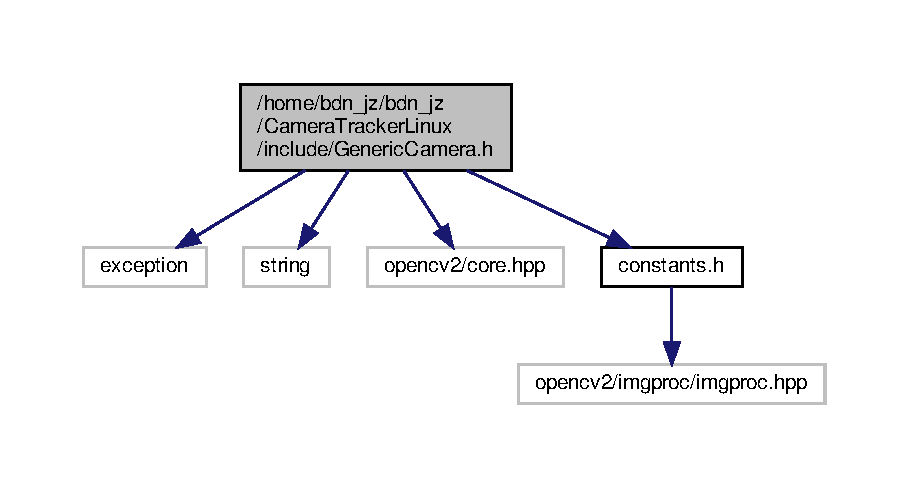
\includegraphics[width=350pt]{_generic_camera_8h__incl}
\end{center}
\end{figure}
This graph shows which files directly or indirectly include this file\+:
\nopagebreak
\begin{figure}[H]
\begin{center}
\leavevmode
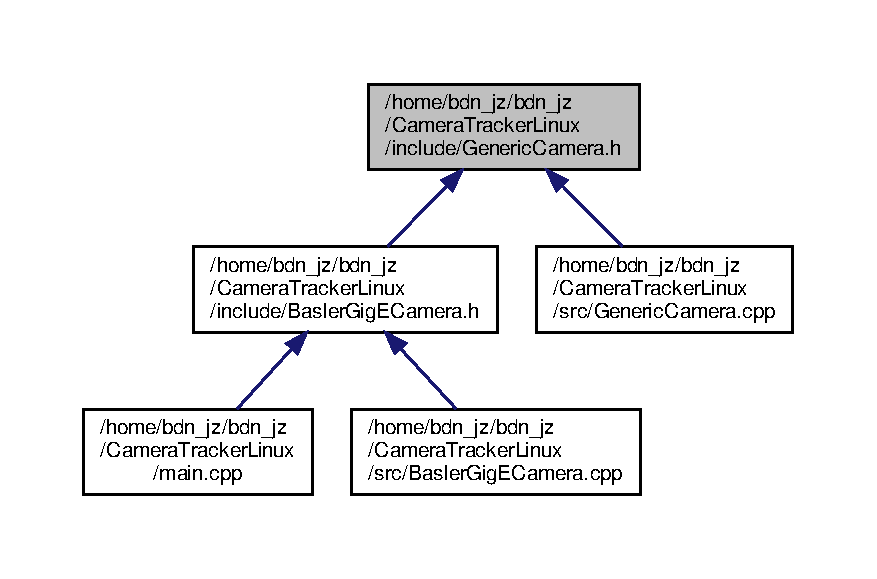
\includegraphics[width=350pt]{_generic_camera_8h__dep__incl}
\end{center}
\end{figure}
\subsection*{Classes}
\begin{DoxyCompactItemize}
\item 
class \hyperlink{class_generic_camera}{Generic\+Camera}
\begin{DoxyCompactList}\small\item\em abstract camera base class. \end{DoxyCompactList}\item 
class \hyperlink{class_generic_camera_1_1disconnected__exception}{Generic\+Camera\+::disconnected\+\_\+exception}
\begin{DoxyCompactList}\small\item\em Exception if device is is disconnected Exception specificly for device disconnection, inherits from std exeception. \end{DoxyCompactList}\end{DoxyCompactItemize}


\subsection{Detailed Description}
Header of the camera base class. 

Header file defining the abstract base class for any kind of camera devices \begin{DoxyAuthor}{Author}
Benjamin Montavon 
\end{DoxyAuthor}
\begin{DoxyDate}{Date}
27.\+11.\+2015 
\end{DoxyDate}

\hypertarget{_rotation_stage_8h}{}\section{/home/bdn\+\_\+jz/bdn\+\_\+jz/camera-\/tracker-\/cpp/\+Camera\+Tracker\+Linux/include/\+Rotation\+Stage.h File Reference}
\label{_rotation_stage_8h}\index{/home/bdn\+\_\+jz/bdn\+\_\+jz/camera-\/tracker-\/cpp/\+Camera\+Tracker\+Linux/include/\+Rotation\+Stage.\+h@{/home/bdn\+\_\+jz/bdn\+\_\+jz/camera-\/tracker-\/cpp/\+Camera\+Tracker\+Linux/include/\+Rotation\+Stage.\+h}}


This file contains the declaration of the \hyperlink{class_rotation_stage}{Rotation\+Stage} class.  


{\ttfamily \#include $<$string$>$}\newline
{\ttfamily \#include $<$iostream$>$}\newline
{\ttfamily \#include \char`\"{}Conex.\+h\char`\"{}}\newline
{\ttfamily \#include $<$fcntl.\+h$>$}\newline
{\ttfamily \#include $<$errno.\+h$>$}\newline
{\ttfamily \#include $<$termios.\+h$>$}\newline
{\ttfamily \#include $<$unistd.\+h$>$}\newline
Include dependency graph for Rotation\+Stage.\+h\+:
\nopagebreak
\begin{figure}[H]
\begin{center}
\leavevmode
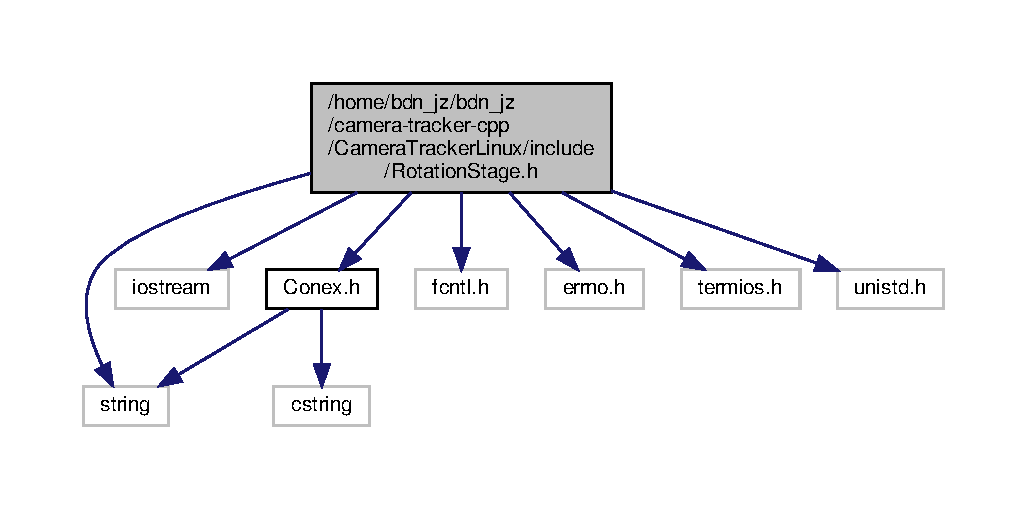
\includegraphics[width=350pt]{_rotation_stage_8h__incl}
\end{center}
\end{figure}
This graph shows which files directly or indirectly include this file\+:
\nopagebreak
\begin{figure}[H]
\begin{center}
\leavevmode
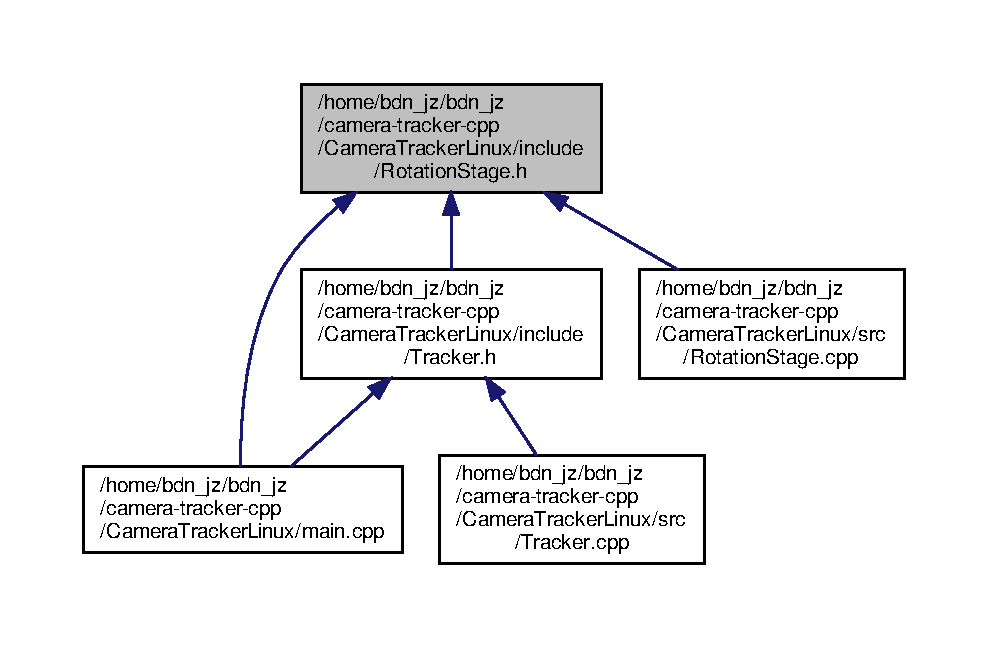
\includegraphics[width=350pt]{_rotation_stage_8h__dep__incl}
\end{center}
\end{figure}
\subsection*{Classes}
\begin{DoxyCompactItemize}
\item 
class \hyperlink{class_rotation_stage}{Rotation\+Stage}
\end{DoxyCompactItemize}


\subsection{Detailed Description}
This file contains the declaration of the \hyperlink{class_rotation_stage}{Rotation\+Stage} class. 

\begin{DoxyAuthor}{Author}
Jiancong Zheng 
\end{DoxyAuthor}
\begin{DoxyDate}{Date}
2020-\/06-\/10 
\end{DoxyDate}

\hypertarget{_scanner_8h}{}\section{/home/bdn\+\_\+jz/bdn\+\_\+jz/camera-\/tracker-\/cpp/\+Camera\+Tracker\+Linux/include/\+Scanner.h File Reference}
\label{_scanner_8h}\index{/home/bdn\+\_\+jz/bdn\+\_\+jz/camera-\/tracker-\/cpp/\+Camera\+Tracker\+Linux/include/\+Scanner.\+h@{/home/bdn\+\_\+jz/bdn\+\_\+jz/camera-\/tracker-\/cpp/\+Camera\+Tracker\+Linux/include/\+Scanner.\+h}}


This file contains the declaration of the Scanner class.  


{\ttfamily \#include $<$zbar.\+h$>$}\newline
{\ttfamily \#include \char`\"{}Chessboard\+Detector.\+h\char`\"{}}\newline
Include dependency graph for Scanner.\+h\+:
\nopagebreak
\begin{figure}[H]
\begin{center}
\leavevmode
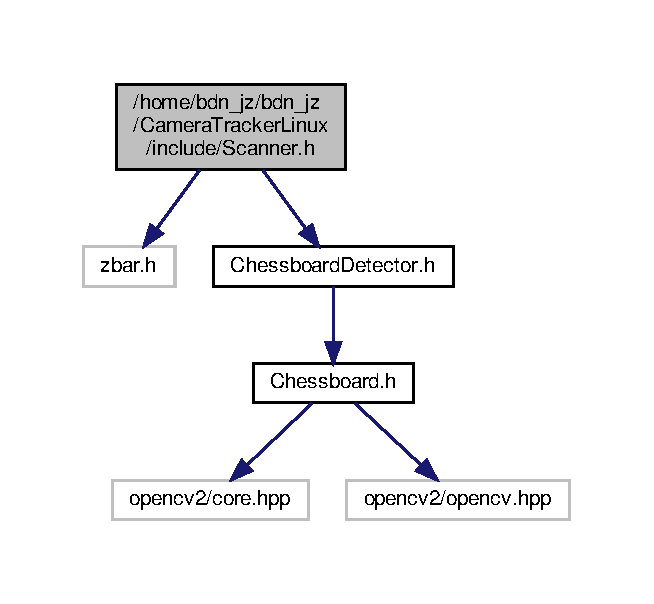
\includegraphics[width=350pt]{_scanner_8h__incl}
\end{center}
\end{figure}
This graph shows which files directly or indirectly include this file\+:
\nopagebreak
\begin{figure}[H]
\begin{center}
\leavevmode
\includegraphics[width=350pt]{_scanner_8h__dep__incl}
\end{center}
\end{figure}
\subsection*{Classes}
\begin{DoxyCompactItemize}
\item 
struct \hyperlink{struct_code_info}{Code\+Info}
\begin{DoxyCompactList}\small\item\em Structure that contains the related information of the code. \end{DoxyCompactList}\item 
class \hyperlink{class_code_scanner}{Code\+Scanner}
\begin{DoxyCompactList}\small\item\em Class that contains the precedures of finding the position of code and decoding the code. \end{DoxyCompactList}\item 
class \hyperlink{class_barcode_scanner}{Barcode\+Scanner}
\begin{DoxyCompactList}\small\item\em Class that contains the precedures of finding the position of barcode and decoding the barcode. This class is a child class of \hyperlink{class_code_scanner}{Code\+Scanner}. \end{DoxyCompactList}\item 
class \hyperlink{class_qrcode_scanner}{Qrcode\+Scanner}
\begin{DoxyCompactList}\small\item\em Class that contains the precedures of finding the position of Q\+R-\/code and decoding the Q\+R-\/code. This is a child class of \hyperlink{class_code_scanner}{Code\+Scanner}. \end{DoxyCompactList}\end{DoxyCompactItemize}
\subsection*{Typedefs}
\begin{DoxyCompactItemize}
\item 
typedef struct \hyperlink{struct_code_info}{Code\+Info} \hyperlink{_scanner_8h_ac4ad61d97179f5b3fd0c4935060e9217}{Code\+Info}
\end{DoxyCompactItemize}


\subsection{Detailed Description}
This file contains the declaration of the Scanner class. 

\begin{DoxyAuthor}{Author}
Jiancong Zheng 
\end{DoxyAuthor}
\begin{DoxyDate}{Date}
2020-\/05-\/29 
\end{DoxyDate}


\subsection{Typedef Documentation}
\mbox{\Hypertarget{_scanner_8h_ac4ad61d97179f5b3fd0c4935060e9217}\label{_scanner_8h_ac4ad61d97179f5b3fd0c4935060e9217}} 
\index{Scanner.\+h@{Scanner.\+h}!Code\+Info@{Code\+Info}}
\index{Code\+Info@{Code\+Info}!Scanner.\+h@{Scanner.\+h}}
\subsubsection{\texorpdfstring{Code\+Info}{CodeInfo}}
{\footnotesize\ttfamily typedef struct \hyperlink{struct_code_info}{Code\+Info}  \hyperlink{struct_code_info}{Code\+Info}}


\hypertarget{_timed_frame_8h}{}\section{/home/bdn\+\_\+jz/bdn\+\_\+jz/camera-\/tracker-\/cpp/\+Camera\+Tracker\+Linux/include/\+Timed\+Frame.h File Reference}
\label{_timed_frame_8h}\index{/home/bdn\+\_\+jz/bdn\+\_\+jz/camera-\/tracker-\/cpp/\+Camera\+Tracker\+Linux/include/\+Timed\+Frame.\+h@{/home/bdn\+\_\+jz/bdn\+\_\+jz/camera-\/tracker-\/cpp/\+Camera\+Tracker\+Linux/include/\+Timed\+Frame.\+h}}
{\ttfamily \#include $<$opencv2/core.\+hpp$>$}\newline
Include dependency graph for Timed\+Frame.\+h\+:
\nopagebreak
\begin{figure}[H]
\begin{center}
\leavevmode
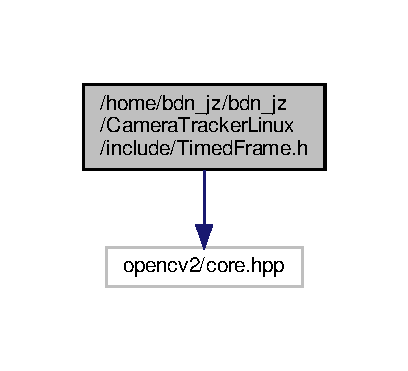
\includegraphics[width=224pt]{_timed_frame_8h__incl}
\end{center}
\end{figure}
This graph shows which files directly or indirectly include this file\+:
\nopagebreak
\begin{figure}[H]
\begin{center}
\leavevmode
\includegraphics[width=350pt]{_timed_frame_8h__dep__incl}
\end{center}
\end{figure}
\subsection*{Classes}
\begin{DoxyCompactItemize}
\item 
class \hyperlink{class_timed_frame}{Timed\+Frame}
\end{DoxyCompactItemize}

\hypertarget{main_8cpp}{}\section{/home/bdn\+\_\+jz/bdn\+\_\+jz/camera-\/tracker-\/cpp/\+Camera\+Tracker\+Linux/main.cpp File Reference}
\label{main_8cpp}\index{/home/bdn\+\_\+jz/bdn\+\_\+jz/camera-\/tracker-\/cpp/\+Camera\+Tracker\+Linux/main.\+cpp@{/home/bdn\+\_\+jz/bdn\+\_\+jz/camera-\/tracker-\/cpp/\+Camera\+Tracker\+Linux/main.\+cpp}}
{\ttfamily \#include \char`\"{}Chessboard\+Detector.\+h\char`\"{}}\newline
{\ttfamily \#include \char`\"{}Basler\+Gig\+E\+Camera.\+h\char`\"{}}\newline
{\ttfamily \#include \char`\"{}Scanner.\+h\char`\"{}}\newline
{\ttfamily \#include \char`\"{}Rotation\+Stage.\+h\char`\"{}}\newline
{\ttfamily \#include \char`\"{}Pose\+Estimation.\+h\char`\"{}}\newline
{\ttfamily \#include \char`\"{}Tracker.\+h\char`\"{}}\newline
Include dependency graph for main.\+cpp\+:
\nopagebreak
\begin{figure}[H]
\begin{center}
\leavevmode
\includegraphics[width=350pt]{main_8cpp__incl}
\end{center}
\end{figure}
\subsection*{Functions}
\begin{DoxyCompactItemize}
\item 
int \hyperlink{main_8cpp_ae66f6b31b5ad750f1fe042a706a4e3d4}{main} ()
\end{DoxyCompactItemize}


\subsection{Function Documentation}
\mbox{\Hypertarget{main_8cpp_ae66f6b31b5ad750f1fe042a706a4e3d4}\label{main_8cpp_ae66f6b31b5ad750f1fe042a706a4e3d4}} 
\index{main.\+cpp@{main.\+cpp}!main@{main}}
\index{main@{main}!main.\+cpp@{main.\+cpp}}
\subsubsection{\texorpdfstring{main()}{main()}}
{\footnotesize\ttfamily int main (\begin{DoxyParamCaption}{ }\end{DoxyParamCaption})}


\hypertarget{_r_e_a_d_m_e_8md}{}\section{/home/bdn\+\_\+jz/bdn\+\_\+jz/camera-\/tracker-\/cpp/\+Camera\+Tracker\+Linux/\+R\+E\+A\+D\+ME.md File Reference}
\label{_r_e_a_d_m_e_8md}\index{/home/bdn\+\_\+jz/bdn\+\_\+jz/camera-\/tracker-\/cpp/\+Camera\+Tracker\+Linux/\+R\+E\+A\+D\+M\+E.\+md@{/home/bdn\+\_\+jz/bdn\+\_\+jz/camera-\/tracker-\/cpp/\+Camera\+Tracker\+Linux/\+R\+E\+A\+D\+M\+E.\+md}}

\hypertarget{_basler_gig_e_camera_8cpp}{}\section{/home/jc/\+H\+I\+W\+I/camera-\/tracker-\/cpp/\+Camera\+Tracker\+Linux/src/\+Basler\+Gig\+E\+Camera.cpp File Reference}
\label{_basler_gig_e_camera_8cpp}\index{/home/jc/\+H\+I\+W\+I/camera-\/tracker-\/cpp/\+Camera\+Tracker\+Linux/src/\+Basler\+Gig\+E\+Camera.\+cpp@{/home/jc/\+H\+I\+W\+I/camera-\/tracker-\/cpp/\+Camera\+Tracker\+Linux/src/\+Basler\+Gig\+E\+Camera.\+cpp}}


Body file for the Basler GigE Camera class.  


{\ttfamily \#include $<$chrono$>$}\\*
{\ttfamily \#include \char`\"{}constants.\+h\char`\"{}}\\*
{\ttfamily \#include \char`\"{}Basler\+Gig\+E\+Camera.\+h\char`\"{}}\\*
{\ttfamily \#include $<$pylon/\+Pylon\+Utility\+Includes.\+h$>$}\\*
Include dependency graph for Basler\+Gig\+E\+Camera.\+cpp\+:
% FIG 0


\subsection{Detailed Description}
Body file for the Basler GigE Camera class. 

File that contains the implementation of the Basler GigE Camera class. It relies on Pylon/\+Basler inlcudes but not on Qt. \begin{DoxyAuthor}{Author}
Benjamin Montavon 
\end{DoxyAuthor}
\begin{DoxyDate}{Date}
27.\+11.\+2015 
\end{DoxyDate}

\hypertarget{_chessboard_8cpp}{}\section{/home/bdn\+\_\+jz/bdn\+\_\+jz/\+Camera\+Tracker\+Linux/src/\+Chessboard.cpp File Reference}
\label{_chessboard_8cpp}\index{/home/bdn\+\_\+jz/bdn\+\_\+jz/\+Camera\+Tracker\+Linux/src/\+Chessboard.\+cpp@{/home/bdn\+\_\+jz/bdn\+\_\+jz/\+Camera\+Tracker\+Linux/src/\+Chessboard.\+cpp}}
{\ttfamily \#include \char`\"{}Chessboard.\+h\char`\"{}}\newline
Include dependency graph for Chessboard.\+cpp\+:\nopagebreak
\begin{figure}[H]
\begin{center}
\leavevmode
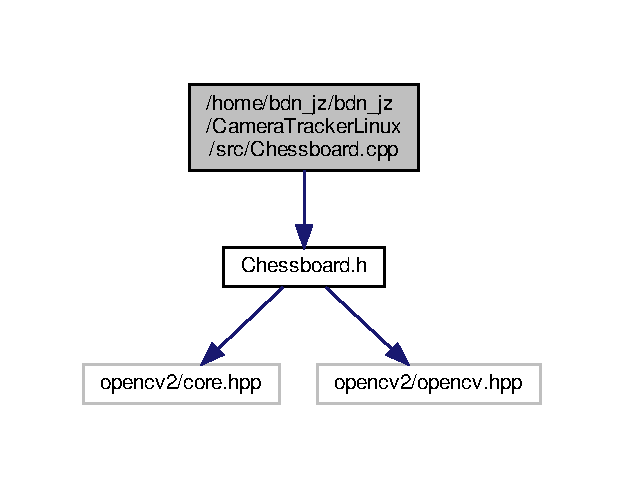
\includegraphics[width=300pt]{_chessboard_8cpp__incl}
\end{center}
\end{figure}

\hypertarget{_chessboard_detector_8cpp}{}\section{/home/bdn\+\_\+jz/bdn\+\_\+jz/camera-\/tracker-\/cpp/\+Camera\+Tracker\+Linux/src/\+Chessboard\+Detector.cpp File Reference}
\label{_chessboard_detector_8cpp}\index{/home/bdn\+\_\+jz/bdn\+\_\+jz/camera-\/tracker-\/cpp/\+Camera\+Tracker\+Linux/src/\+Chessboard\+Detector.\+cpp@{/home/bdn\+\_\+jz/bdn\+\_\+jz/camera-\/tracker-\/cpp/\+Camera\+Tracker\+Linux/src/\+Chessboard\+Detector.\+cpp}}
{\ttfamily \#include \char`\"{}Chessboard\+Detector.\+h\char`\"{}}\newline
Include dependency graph for Chessboard\+Detector.\+cpp\+:
\nopagebreak
\begin{figure}[H]
\begin{center}
\leavevmode
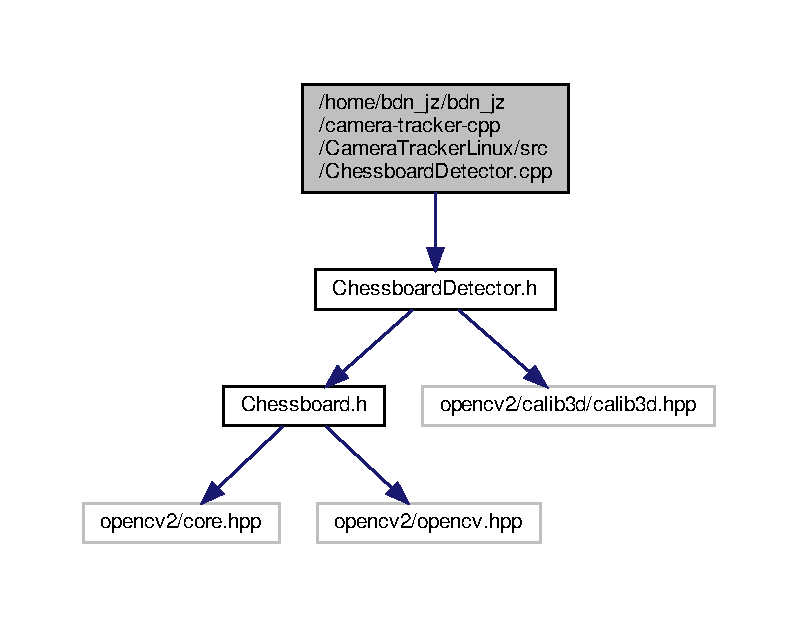
\includegraphics[width=300pt]{_chessboard_detector_8cpp__incl}
\end{center}
\end{figure}

\hypertarget{_conex_8cpp}{}\section{/home/bdn\+\_\+jz/bdn\+\_\+jz/camera-\/tracker-\/cpp/\+Camera\+Tracker\+Linux/src/\+Conex.cpp File Reference}
\label{_conex_8cpp}\index{/home/bdn\+\_\+jz/bdn\+\_\+jz/camera-\/tracker-\/cpp/\+Camera\+Tracker\+Linux/src/\+Conex.\+cpp@{/home/bdn\+\_\+jz/bdn\+\_\+jz/camera-\/tracker-\/cpp/\+Camera\+Tracker\+Linux/src/\+Conex.\+cpp}}
{\ttfamily \#include \char`\"{}Conex.\+h\char`\"{}}\newline
Include dependency graph for Conex.\+cpp\+:\nopagebreak
\begin{figure}[H]
\begin{center}
\leavevmode
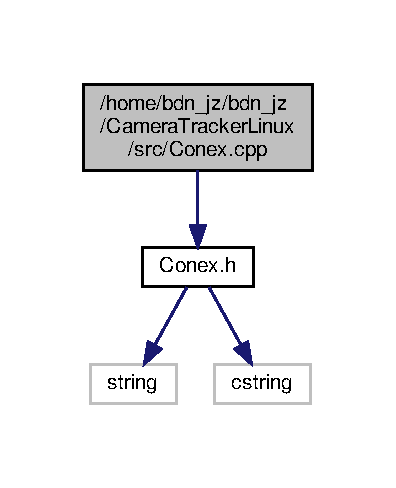
\includegraphics[width=207pt]{_conex_8cpp__incl}
\end{center}
\end{figure}

\hypertarget{_generic_camera_8cpp}{}\section{/home/bdn\+\_\+jz/bdn\+\_\+jz/camera-\/tracker-\/cpp/\+Camera\+Tracker\+Linux/src/\+Generic\+Camera.cpp File Reference}
\label{_generic_camera_8cpp}\index{/home/bdn\+\_\+jz/bdn\+\_\+jz/camera-\/tracker-\/cpp/\+Camera\+Tracker\+Linux/src/\+Generic\+Camera.\+cpp@{/home/bdn\+\_\+jz/bdn\+\_\+jz/camera-\/tracker-\/cpp/\+Camera\+Tracker\+Linux/src/\+Generic\+Camera.\+cpp}}


Boday of the camera base class.  


{\ttfamily \#include \char`\"{}constants.\+h\char`\"{}}\newline
{\ttfamily \#include \char`\"{}Generic\+Camera.\+h\char`\"{}}\newline
Include dependency graph for Generic\+Camera.\+cpp\+:
\nopagebreak
\begin{figure}[H]
\begin{center}
\leavevmode
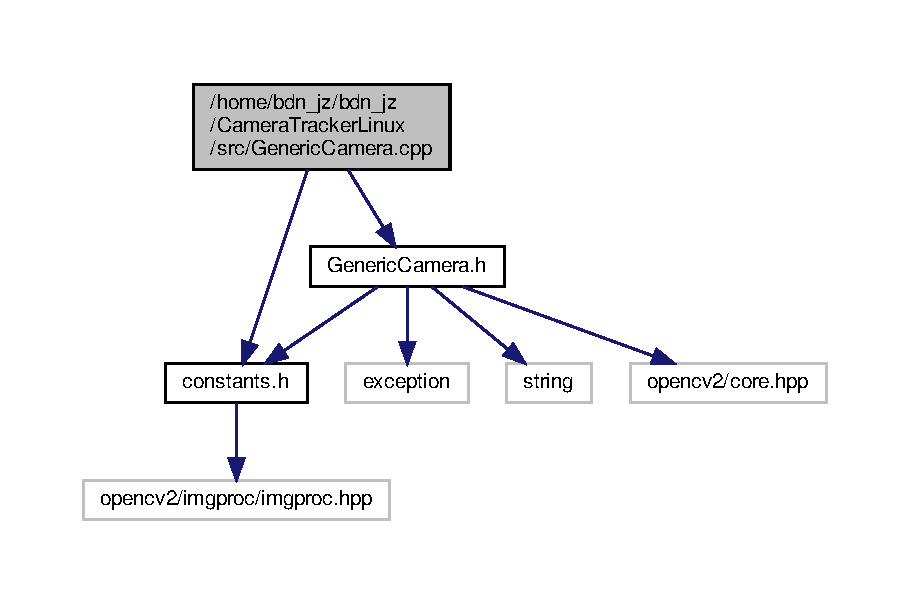
\includegraphics[width=350pt]{_generic_camera_8cpp__incl}
\end{center}
\end{figure}


\subsection{Detailed Description}
Boday of the camera base class. 

File implementing the abstract base class functions for any kind of camera devices \begin{DoxyAuthor}{Author}
Benjamin Montavon 
\end{DoxyAuthor}
\begin{DoxyDate}{Date}
27.\+11.\+2015 
\end{DoxyDate}

\hypertarget{_rotation_stage_8cpp}{}\section{/home/bdn\+\_\+jz/bdn\+\_\+jz/\+Camera\+Tracker\+Linux/src/\+Rotation\+Stage.cpp File Reference}
\label{_rotation_stage_8cpp}\index{/home/bdn\+\_\+jz/bdn\+\_\+jz/\+Camera\+Tracker\+Linux/src/\+Rotation\+Stage.\+cpp@{/home/bdn\+\_\+jz/bdn\+\_\+jz/\+Camera\+Tracker\+Linux/src/\+Rotation\+Stage.\+cpp}}
{\ttfamily \#include \char`\"{}Rotation\+Stage.\+h\char`\"{}}\newline
Include dependency graph for Rotation\+Stage.\+cpp\+:\nopagebreak
\begin{figure}[H]
\begin{center}
\leavevmode
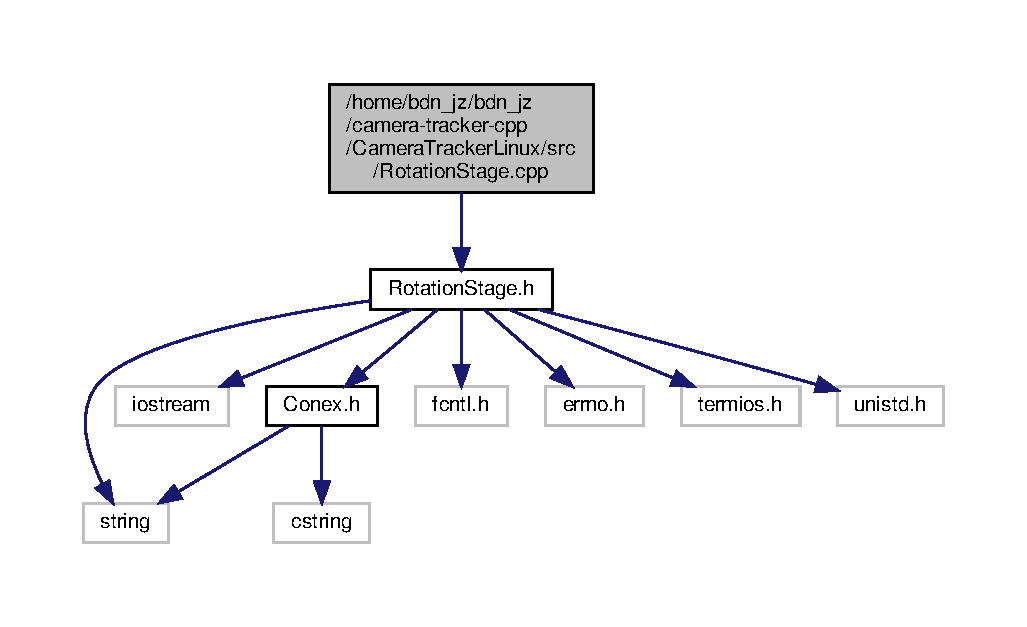
\includegraphics[width=350pt]{_rotation_stage_8cpp__incl}
\end{center}
\end{figure}

\hypertarget{_scanner_8cpp}{}\section{/home/jc/\+H\+I\+W\+I/camera-\/tracker-\/cpp/\+Camera\+Tracker\+Linux/src/\+Scanner.cpp File Reference}
\label{_scanner_8cpp}\index{/home/jc/\+H\+I\+W\+I/camera-\/tracker-\/cpp/\+Camera\+Tracker\+Linux/src/\+Scanner.\+cpp@{/home/jc/\+H\+I\+W\+I/camera-\/tracker-\/cpp/\+Camera\+Tracker\+Linux/src/\+Scanner.\+cpp}}
{\ttfamily \#include \char`\"{}Scanner.\+h\char`\"{}}\\*
Include dependency graph for Scanner.\+cpp\+:
% FIG 0

\hypertarget{_timed_frame_8cpp}{}\section{/home/bdn\+\_\+jz/bdn\+\_\+jz/camera-\/tracker-\/cpp/\+Camera\+Tracker\+Linux/src/\+Timed\+Frame.cpp File Reference}
\label{_timed_frame_8cpp}\index{/home/bdn\+\_\+jz/bdn\+\_\+jz/camera-\/tracker-\/cpp/\+Camera\+Tracker\+Linux/src/\+Timed\+Frame.\+cpp@{/home/bdn\+\_\+jz/bdn\+\_\+jz/camera-\/tracker-\/cpp/\+Camera\+Tracker\+Linux/src/\+Timed\+Frame.\+cpp}}
{\ttfamily \#include \char`\"{}Timed\+Frame.\+h\char`\"{}}\newline
Include dependency graph for Timed\+Frame.\+cpp\+:\nopagebreak
\begin{figure}[H]
\begin{center}
\leavevmode
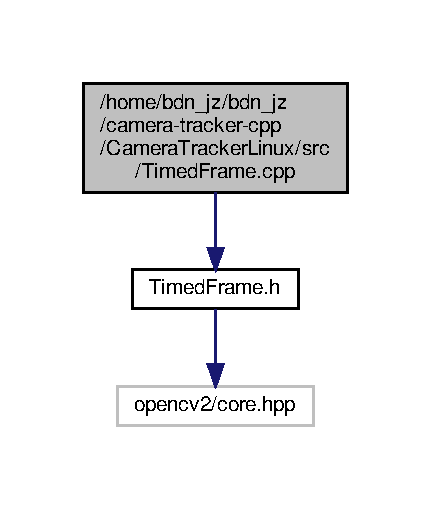
\includegraphics[width=207pt]{_timed_frame_8cpp__incl}
\end{center}
\end{figure}

%--- End generated contents ---

% Index
\backmatter
\newpage
\phantomsection
\clearemptydoublepage
\addcontentsline{toc}{chapter}{Index}
\printindex

\end{document}
